\documentclass[11pt]{report}

\usepackage[T1]{fontenc}
\usepackage[margin=1in]{geometry}
\usepackage{amsmath, amssymb, amsthm}
\usepackage{enumitem}
\usepackage{hyperref}
\usepackage{booktabs}
\usepackage{listings}
\usepackage{xcolor}
\usepackage{standalone}
\usepackage{makeidx}
\makeindex

\lstset{
  basicstyle=\ttfamily\small,
  frame=single,
  breaklines=true,
  columns=fullflexible,
  mathescape=true
}

\theoremstyle{definition}
\newtheorem{theorem}{Theorem}[section]
\newtheorem{definition}[theorem]{Definition}
\newtheorem{example}[theorem]{Example}

\hypersetup{
  colorlinks=true,
  linkcolor=blue!60!black,
  urlcolor=blue!60!black
}

\title{CS 250: Introduction to Logic and\\Mathematical Reasoning\\[10pt]\large Course Notes}
\author{}
\date{}

\begin{document}
\pagenumbering{gobble}
\maketitle
\clearpage
\pagenumbering{roman}
\tableofcontents
\clearpage
\pagenumbering{arabic}

% Suppress \maketitle in included module files
\def\maketitle{}

\chapter{Welcome, Sets, and Functions}
\documentclass[11pt]{article}

% cs250preamble.tex --- shared preamble for CS 250 course notes
%
% This file is \input by main.tex and by each individual module
% file so that each module can still compile standalone. Any
% package or custom-environment change should be made here, not
% in the individual module files.

\usepackage[T1]{fontenc}
\usepackage[margin=1in]{geometry}
\usepackage{amsmath, amssymb, amsthm}
\usepackage{enumitem}
\usepackage{hyperref}
\usepackage{booktabs}
\usepackage{listings}
\usepackage{xcolor}
\usepackage{tikz}
\usetikzlibrary{shapes.geometric, shapes.gates.logic.US, shapes.gates.logic.IEC, arrows.meta, positioning, calc, trees}
\usepackage{bussproofs}
\usepackage{mdframed}

\lstset{
  basicstyle=\ttfamily\small,
  frame=single,
  breaklines=true,
  columns=fullflexible,
  mathescape=true
}

\theoremstyle{definition}
\newtheorem{theorem}{Theorem}[section]
\newtheorem{definition}[theorem]{Definition}
\newtheorem{example}[theorem]{Example}

\hypersetup{
  colorlinks=true,
  linkcolor=blue!60!black,
  urlcolor=blue!60!black
}

% Key-takeaway box: used at the end of major sections and at the end of
% each module to summarise the main points. Expects \item bullets inside.
\newmdenv[
  linewidth=0.8pt,
  linecolor=blue!40!black,
  backgroundcolor=blue!3,
  skipabove=8pt,
  skipbelow=8pt,
  innertopmargin=7pt,
  innerbottommargin=7pt,
  innerleftmargin=9pt,
  innerrightmargin=9pt
]{keytakeawaybox}
\newenvironment{keytakeaway}{%
  \begin{keytakeawaybox}%
  \noindent\textbf{Key takeaways.}%
  \begin{itemize}[leftmargin=1.3em, topsep=2pt, itemsep=1pt, label=\textbullet]%
}{%
  \end{itemize}%
  \end{keytakeawaybox}%
}

% Summary/looking-ahead environment: used once at the end of each module
% to wrap up what the module built and point forward.
\newmdenv[
  linewidth=0.8pt,
  linecolor=gray!60,
  backgroundcolor=gray!5,
  skipabove=8pt,
  skipbelow=8pt,
  innertopmargin=7pt,
  innerbottommargin=7pt,
  innerleftmargin=9pt,
  innerrightmargin=9pt
]{summarybox}

% Sidebar environment: used for tangential asides---historical notes,
% pointers to other areas of math/CS, cross-paradigm remarks---that
% enrich the main narrative without being essential to it. Takes one
% argument: the sidebar's title.
\newmdenv[
  linewidth=0.6pt,
  linecolor=gray!60,
  backgroundcolor=gray!4,
  skipabove=8pt,
  skipbelow=8pt,
  innertopmargin=6pt,
  innerbottommargin=6pt,
  innerleftmargin=9pt,
  innerrightmargin=9pt
]{sidebarbox}
\newenvironment{sidebar}[1]{%
  \begin{sidebarbox}%
  \noindent\textbf{Sidebar: #1.}\par\medskip%
}{%
  \end{sidebarbox}%
}

% Reading-map environment: used at the top of each numbered module to
% indicate Epp coverage, prerequisites, relevant intermezzi, and
% suggested practice problems. Expects four \rmentry{label}{body}
% items inside (or arbitrary paragraphs).
\newmdenv[
  linewidth=0.8pt,
  linecolor=black!55,
  backgroundcolor=yellow!4,
  skipabove=10pt,
  skipbelow=14pt,
  innertopmargin=9pt,
  innerbottommargin=9pt,
  innerleftmargin=11pt,
  innerrightmargin=11pt
]{readingmapbox}
\newcommand{\rmentry}[2]{\par\noindent\textbf{#1}\hspace{0.4em}#2\par}
\newenvironment{readingmap}{%
  \begin{readingmapbox}%
  \noindent{\bfseries\large Reading map}%
  \vspace{2pt}%
  \setlength{\parskip}{4pt plus 1pt}%
}{%
  \end{readingmapbox}%
}


\title{CS 250 --- Module 1: Welcome, Sets, and Functions}
\author{}
\date{}

\begin{document}
\maketitle

\begin{readingmap}
\rmentry{Epp sections.}{§1.1--1.3: the language of sets, the language of relations and functions, and the language of variables. Module 1's job is to build the shared vocabulary that every later module will reuse.}

\rmentry{Prerequisites.}{None---this is where the book starts. Comfort with a little Python or similar programming will help the aside-style examples feel familiar but is not required.}

\rmentry{Relevant intermezzi.}{``How to Write a Proof'' immediately follows this module and is deliberately short---revisit it while working the exercises below. ``Cardinality and Function Spaces'' (the set-theory intermezzo after it) uses this module's vocabulary to show that some infinities are genuinely bigger than others.}

\rmentry{Practice from Epp.}{§1.1 exercises on set notation, set-builder notation, and set operations; §1.2 exercises on identifying functions, domains/codomains, and injections/surjections; §1.3 exercises on reflexive/symmetric/transitive relations. A runnable Python companion for this module lives at \texttt{code/module01\_sets.py}.}
\end{readingmap}

\section{A Note on The Textbook}
If you're having trouble finding a copy of Epp 5th edition, check the library, course reserves, or the instructor first. Older editions can also still be useful for extra practice problems.

\section{Welcome to CS 250}
Welcome to CS 250! This class is an introduction to logic and mathematical reasoning geared towards computer scientists. By the end of it you will
\begin{itemize}
  \item Be able to explain what a mathematical proof is
  \item Know the distinction between formal and informal proofs
  \item Be able to prove mathematical and logical statements with direct and indirect proof methods
  \item Be able to calculate truth tables for Boolean expressions
  \item Be able to define data in BNF notation
  \item Be able to explain the induction principle on the natural numbers
  \item Know how to relate induction on other types to natural induction
  \item Be able to perform simple formal proofs of program correctness
\end{itemize}

\subsection*{A note on the structure of these notes}
Between the main modules you'll find \emph{intermezzi}---short chapters on topics that are more mathematically sophisticated, that go deeper into a subject than the main modules require, or that cover optional material you may find interesting. They are unnumbered and won't appear on exams unless your instructor says otherwise. Think of them as the bonus tracks on an album: they enrich the experience but the main story is told in the numbered modules.

\section{Why study logic?}
\begin{itemize}
  \item understanding how to write proofs will let you reason about the \emph{limits} of computation
  \item learning logic will help you reason, in general
  \item on a practical level, ``formal methods''---the application of logic to computer science---are a lucrative and in-demand field in high-stakes computing and engineering, from embedded systems programming to chip design to the development of operating system components
\end{itemize}

Take that first point. If we want to understand not just what computers can do \emph{today} but what computers can do \emph{ever}, we need to start with an \textbf{abstract} model of computation---one that doesn't depend on a particular chip architecture or instruction set. Here's the kind of question we'd like to be able to answer: suppose I managed to demonstrate that \textbf{no} AMD chip today could run a program that reads in the code of another program and prints \texttt{1} if that program would run in finite time and \texttt{0} if it would go into an infinite loop. What would that tell us? How do I know there \emph{won't} be a chip that \emph{could} run such a program---maybe a quantum computer, or some architecture we haven't invented yet?

Or consider two programming languages, Python and C. If I can solve a problem in Python, do I \textbf{know} that I can always write a C program that computes the same thing? What about the other way around? We all intuitively feel there isn't a real difference between what two languages can compute---only in how efficiently they compute. But intuition alone isn't good enough for a computer scientist. We need to be able to \emph{know} whether two languages are essentially equivalent, or whether two chips are capable of running the same kinds of programs.

To do that we need mathematical \emph{models} of computation that don't depend on any of these details: not on a specific language, not on specific hardware. We need a model that \emph{abstracts} over those details. Such a model can't be a concrete programming language with a compiler---we've already ruled that out---so instead we'll reason with mathematical tools: sets, symbols, syntax and semantics, proofs. The question ``what is a proof and how do I write one'' is the bulk of this class; the actual mathematical modeling of computation we'll leave for the sequel course, CS 251. For now, I'll say that a proof is a way to convince the reader, by clearly outlining a sequence of reasoning steps, that something is true.

Points two and three are intertwined, and both come down to the difference between \emph{formal} and \emph{informal} proof. Normal proofs, like what I was talking about above, are technically considered ``informal.'' An informal proof is meant to communicate between mathematicians, using a mix of symbolic notation and prose. A formal proof, by contrast, lives \emph{inside} a logic and uses only the logic's own rules. The formal rules of a logic will feel strange and constraining---almost like writing assembly instead of a regular programming language, where each step is small, tedious, and verbose. Yet there's something important you learn by doing it. Again like assembly, you learn \emph{why} things work the way they do. You'll learn how the rules of a logic are justified mathematically, and how those rules help us distinguish good proofs from bad ones. One of the hardest things when you're first writing informal proofs is knowing what you're allowed to say and what needs justification; formal logic helps you build that judgment even when you're not using it directly.

Formal logic isn't just a training exercise you discard once you've learned the basics. Formal proofs resist the kind of errors that are easy to make informally---errors that even professional mathematicians regularly commit. What if you could get those advantages without the tedium? That's where \emph{interactive theorem provers}, sometimes called proof assistants, come in. These are like very specialized programming languages where the programs you write \emph{are also} proofs in a formal logic. Using a proof assistant is its own skill, and becoming truly competent with one is beyond the scope of this course, but I at least want to expose you to using them.

\section{What is logic, what is a proof?}
Let's make the central concept of this course precise. Logic is the study of how the truth of statements follows from their premises by means of \emph{valid arguments}---arguments built from correct reasoning steps. In mathematics, we call a valid argument a \emph{proof}: a way to convince the reader, through a clear sequence of reasoning steps, that something is true. Let's see what that looks like in practice with a simple example.

Say you were thinking about the \emph{natural numbers}---the numbers that are either zero or a positive whole number. You realize ``hey, there are a lot of these. There must be infinitely many of them,'' and now you want to convince yourself this is \emph{true}. In other words, you want to \emph{prove} it.

To start, you have a rather clever guess on how to show this. First, you note that if you have a natural number you can always add one and it stays a positive whole number. Second, you decide to see what happens if there's a \textbf{finite} amount of natural numbers. You're going to \emph{assume} that this is true and then see if you can show it leads to something weird.

The first consequence of there being a \emph{finite} number of natural numbers is that there must be a \emph{biggest} natural number.

Why? Because for any two natural numbers one of them must be at least as large as the other. If you compare all of these finite numbers, one of them must be the biggest.\footnote{Can you implement this idea as a program?}

Then if we have a biggest natural number we should be able to add one to it and get a new natural number. This new natural number must be bigger.

But how can this be true if we already found the biggest?

We've found a contradiction. A contradiction usually means something has gone wrong---and something has: our assumption that there are only finitely many naturals. Since the assumption leads to nonsense, we conclude that there are \emph{infinitely many} natural numbers.

We've proved what we set out to prove, then, that there are \emph{infinitely many natural numbers}.

This is a pretty valid proof by mathematician standards, but let's talk about some of the assumptions that went into it:

\begin{itemize}
  \item First, we didn't actually show that you always get a new natural number by adding one to a natural number; we just appealed to the intuition that we've all done addition before and asserted it.
  \item Second, we didn't actually explain how we can generalize from ``you can always compare two numbers'' to ``you can compare all the numbers in a collection of numbers.''
  \item Third, we didn't even technically define what comparing the size of two numbers means. Did you catch that?
  \item Finally, we didn't actually justify this proof by contradiction technique. How do we know that just because we've found a contradiction from the assumption that the natural numbers are finite that we absolutely \emph{know} that they must instead be infinite? We didn't even define finite and infinite, did we?
\end{itemize}

My point here is that even when a mathematician writes a proof there is usually a body of assumptions, definitions, and facts that they're relying on!

The world's most niche personality test:
\begin{itemize}
  \item If you're completely unbothered by these omissions, you're thinking like a mathematician: focused on getting the right intuition and letting some details slide for the sake of clarity. You want to finish the proof and move on to the next interesting thing.
  \item If you \textbf{are} bothered, you're thinking like a logician: concerned about getting every detail of a proof correct and being explicit about all assumptions and definitions. You worry about whether things like ``proof by contradiction'' even make sense as a way of acquiring knowledge. You might like the word ``epistemology.''
  \item If you thought ``well I know there are infinitely many natural numbers because I could write a loop that runs forever enumerating them,'' you're thinking like a \emph{constructive} mathematician: a blend of mathematician, logician, and computer scientist. You do math in your code and code with your math. You may have heard of languages like Agda and Idris that blur the line between proof and program.
\end{itemize}

None of these approaches is better than the others; each has its own strengths and weaknesses.

These notes were, however, written by a constructive mathematician, so there may be bias peeking through in how this material is presented.

\section{Variables and formulae}
We've given a proof in a very \emph{informal}, natural-language way. By natural language I mean human language that evolved organically, as opposed to the language of mathematics or a programming language. We need to start moving from this informal language into \emph{formal} language: symbols with rigid meaning. We'll make this journey piecemeal over time, learning how to take statements in human language---which can be ambiguous---and turn them into rigorous, unmistakable combinations of symbols. This will both help us be precise in how we do mathematics and help us move our mathematics from pen and paper to computer programs.

The first such formalization is the introduction of \emph{variables}. You've already seen variables in algebra and programming before, although their uses are slightly different from what we're doing here. We're not ``solving for x'' like in algebra, nor are we using variables like labeled containers as in \emph{C}, \emph{Python}, or similar programming languages where the contents of the container can change over time. Instead, think of variables as generalized pronouns---they work a lot like ``it'' or ``this'' in natural language. There are \emph{patterns} to how we introduce them: we name the variable and its scope and then allow ourselves to use it, e.g.\ ``Consider a chicken \textbf{c}, such that \ldots'' or ``For all students \textbf{s} in CS250 \ldots''

For a more concrete example, recall that in the previous section we assumed there was a largest natural number and talked through the rest of the proof from there. With variables, we can say something like: ``Assume there is a largest natural number, \textbf{n}. Then we know that n+1 is also a natural number and that n+1>n, contradicting the assumption that \textbf{n} is largest.'' That's a lot clearer than trying to write it in just words, right? And all we've done is introduce a small abstraction.

We \emph{need} variables to help us write more complicated kinds of logical statements as well. The first kinds we're going to talk about are what Epp calls universal, existential, and conditional. Universal statements are things like ``all dogs are mammals'' or ``every chicken has a common ancestor''---claims that are true for every possible example of a ``class of thing.'' We're going to make ``class of thing'' more rigorous soon, but for now think ``all dogs,'' ``every person,'' ``all programming languages.'' Universal statements can also include negatives like ``no dogs are also cats'' or ``every person is not immortal.''

Existential statements are like ``there is a smallest natural number'' or ``there is at least one rainy day each fall.'' These are about showing examples of something, or about asserting that a thing with certain properties \emph{exists}---the kinds of claims you make when you're showing a problem even has a solution. For example, ``the equation $3x - 29 = 0$ has a solution'' is an existential statement.

The last kind of statement Epp teases out is the \emph{conditional}, which expresses an ``if-then'' relationship: ``if a pear can be used as a weapon, then it is not ripe,'' or ``if a program does not compile, then it is not correct.'' You can combine all three of these into a single claim---for example, ``for every equation of the form $mx + b = y$, where $m$ is not $0$, there exists a solution,'' which is a universal wrapped around a conditional wrapped around an existential.

We're now ready to make the ``class of thing'' concept a little more formal and talk about \emph{sets}.

\section{Sets and pairs}
In the previous section we talked about classes of things such as ``all dogs'' or ``all C programs''. In mathematics, we call these collections \emph{sets}.

\begin{definition}[Set]
A \emph{set}\index{set} is a collection of objects, called \emph{elements}\index{element}. We denote a set with curly braces \texttt{\{ \}}, with commas separating the elements. If \texttt{x} is an element of set \texttt{A}, we write $x \in A$\index{membership ($\in$)}. If \texttt{x} is not an element of \texttt{A}, we write $x \notin A$.
\end{definition}

Some examples:

\texttt{\{red, green, blue\}}

\texttt{\{you, your friend, your friend's friend\}}

\texttt{\{the best chicken, the worst chicken\}}

These are very \emph{abstract} collections.

How do we make sets? There are three basic ways.
The first is that you can take a finite number of things and put them between the curly braces and call that a set. That's how our first few examples worked.

The second is that you can take \emph{other} sets and then apply a condition---a \emph{predicate}---onto it to make a new set. The easiest example is that you can take $\mathbb{N}$, the set of all natural numbers, and then filter out all the even numbers to get the set of all odd natural numbers. If you've seen Python's ``list comprehensions'' before, then you have seen a similar concept.

In symbols, we denote this with ``set-builder notation''\index{set-builder notation} so we can write the above description as

$\{n \mid n \in \mathbb{N} , n \mathbin{\%} 2 = 1\}$

The general pattern is $\{x \mid x \in S, P(x)\}$, which reads ``the set of all $x$ in $S$ such that $P(x)$ is true.'' The vertical bar $\mid$ means ``such that.''

But how do you get things like ``the set of all natural numbers'' in the first place? That brings us to the third way to define sets, which is \emph{inductively}. We'll introduce this informally by example until the second half of the course, where we make it all more rigorous.

With set-builder notation in hand, we can introduce some basic operations on sets. A standard way to \emph{visualize} these operations is with a \emph{Venn diagram}\index{Venn diagram}: each set is drawn as a circle, and you shade the region corresponding to the set you're describing. Venn diagrams aren't rigorous proofs---they're intuition pumps---but they're enormously useful for figuring out what a set expression \emph{means} before you sit down to verify it.

\begin{definition}[Intersection]
The \emph{intersection}\index{intersection@$\cap$ (intersection)} of two sets $A$ and $B$ is the set of elements they have in common:
$A \cap B := \{ x \mid x \in A \text{ and } x \in B\}$.
\end{definition}

\begin{center}
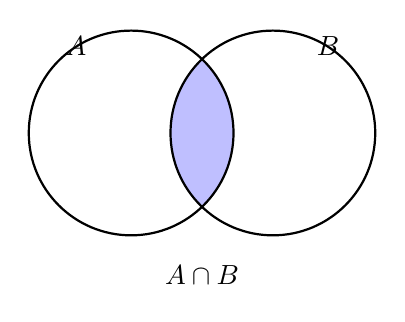
\begin{tikzpicture}
  \begin{scope}
    \clip (-0.9, 0) circle (1.3);
    \fill[blue!25] (0.9, 0) circle (1.3);
  \end{scope}
  \draw[thick] (-0.9, 0) circle (1.3);
  \draw[thick] (0.9, 0) circle (1.3);
  \node at (-1.6, 1.1) {$A$};
  \node at (1.6, 1.1) {$B$};
  \node at (0, -1.8) {$A \cap B$};
\end{tikzpicture}
\end{center}

\begin{definition}[Union]
The \emph{union}\index{union@$\cup$ (union)} of two sets $A$ and $B$ is the set of elements in either $A$ or $B$:
$A \cup B :=  \{ x \mid x \in A \text{ or } x \in B\}$.
\end{definition}

\begin{center}
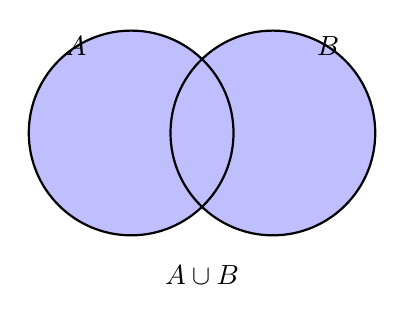
\begin{tikzpicture}
  \fill[blue!25] (-0.9, 0) circle (1.3);
  \fill[blue!25] (0.9, 0) circle (1.3);
  \draw[thick] (-0.9, 0) circle (1.3);
  \draw[thick] (0.9, 0) circle (1.3);
  \node at (-1.6, 1.1) {$A$};
  \node at (1.6, 1.1) {$B$};
  \node at (0, -1.8) {$A \cup B$};
\end{tikzpicture}
\end{center}

\begin{definition}[Subset]
Given sets $A$ and $B$, we say $A$ is a \emph{subset}\index{subset} of $B$, written $A \subseteq B$, when every element of $A$ is also an element of $B$.
\end{definition}

\begin{definition}[Set Difference]
The \emph{difference}\index{set!difference} of sets $A$ and $B$, written $A \setminus B$, is the set of elements in $A$ that are not in $B$:
$A \setminus B := \{x \mid x \in A \text{ and } x \notin B\}$.
\end{definition}

\begin{center}
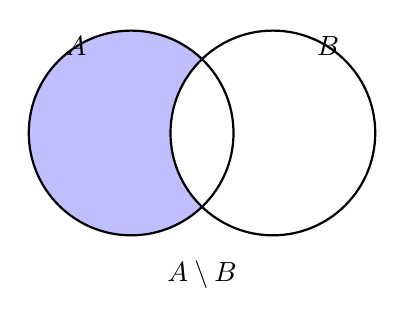
\begin{tikzpicture}
  \begin{scope}
    \clip (-0.9, 0) circle (1.3);
    \fill[blue!25] (-3, -2) rectangle (3, 2);
    \fill[white] (0.9, 0) circle (1.3);
  \end{scope}
  \draw[thick] (-0.9, 0) circle (1.3);
  \draw[thick] (0.9, 0) circle (1.3);
  \node at (-1.6, 1.1) {$A$};
  \node at (1.6, 1.1) {$B$};
  \node at (0, -1.8) {$A \setminus B$};
\end{tikzpicture}
\end{center}

\begin{definition}[Complement]
Given a universal set $U$ that contains all elements under discussion, the \emph{complement}\index{set!complement} of $A$, written $\overline{A}$, is $U \setminus A = \{x \mid x \in U \text{ and } x \notin A\}$.
\end{definition}

\begin{center}
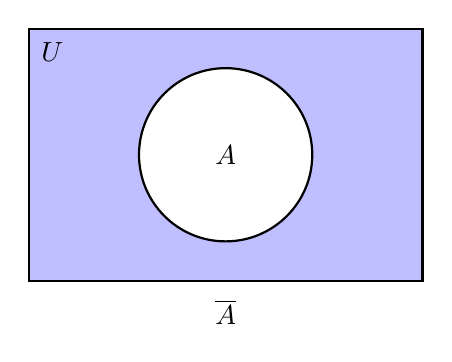
\begin{tikzpicture}
  \fill[blue!25] (-2.5, -1.6) rectangle (2.5, 1.6);
  \fill[white] (0, 0) circle (1.1);
  \draw[thick] (-2.5, -1.6) rectangle (2.5, 1.6);
  \draw[thick] (0, 0) circle (1.1);
  \node at (-2.2, 1.3) {$U$};
  \node at (0, 0) {$A$};
  \node at (0, -2.0) {$\overline{A}$};
\end{tikzpicture}
\end{center}

The complement only makes sense relative to some agreed-upon universe $U$. When we write $\overline{A}$ we're implicitly assuming everyone knows what $U$ is.

A quick notation warning: you'll also see $A^c$\index{complement!notation $A^c$} used for the complement of $A$, particularly in Lean and in the Natural Number Game. The overline and the superscript-$c$ mean the same thing; the choice is a matter of typographic convenience.

\begin{sidebar}{universes, then and now}
The phrase ``universal set'' is doing more work than it lets on. Early set theorists---Cantor, Frege---were happy to talk about \emph{the} universe: the set of absolutely everything. That ran aground on \emph{Russell's paradox}\index{Russell's paradox}: consider the ``set'' of all sets that don't contain themselves. Does it contain itself? Either answer contradicts itself. The moral was that not every predicate carves out a set. Modern axiomatic set theory (ZFC) fixes this by only letting you form $\{x \in S \mid P(x)\}$ relative to some \emph{already-existing} set $S$---exactly the ``subset with a predicate'' construction we've been using. There is no set of all sets in ZFC, so the phrase ``universe $U$'' in the definition of complement is always a stand-in for ``some large enough set we've agreed on for this discussion.''

Category theorists, who genuinely do want to talk about ``all groups'' or ``all topological spaces,'' cope with this by working inside a \emph{Grothendieck universe}\index{Grothendieck universe}---a set big enough to pretend it's everything, while technically sitting inside an even bigger one.

Type theory faces the same problem from a different angle. If you try to have a single type \texttt{Type} that contains all types, including itself, you run into Girard's paradox---a type-theoretic cousin of Russell's. Systems like Coq, Agda, and Lean solve this with a \emph{universe hierarchy}\index{universe hierarchy}: \texttt{Type 0} contains ordinary types, \texttt{Type 1} contains \texttt{Type 0}, and so on up. In practice you rarely see the indices because the elaborator figures them out for you (``universe polymorphism''), but they're always there in the background, preventing the self-referential collapse.

So when these notes say ``universe'' we mean something weaker than a god's-eye view of everything. It just means: a context---a set, a type, a level---big enough to contain what we're talking about today.
\end{sidebar}

\begin{definition}[Disjoint]
Two sets $A$ and $B$ are \emph{disjoint}\index{disjoint} if they share no elements: $A \cap B = \emptyset$.
\end{definition}

Next is something that seems obvious but is incredibly important and---in the history of mathematics---quite divisive: equality of sets.

Two sets are equal exactly when $A \subseteq B$ and $B \subseteq A$, in other words when the two sets have \emph{exactly} the same elements.

This has a couple of implications. First, there's no sense of \emph{ordering} in sets: $\{a,b,c\} = \{c,b,a\} = \{c,a,b\}$. Second, it doesn't matter how you build the sets. You could get the ``set of natural numbers divisible by four'' either as $\{x \mid x \in \mathbb{N}, x \mathbin{\%} 4 = 0\}$ or as a two-step process: first get the even numbers $E = \{x \mid x \in \mathbb{N}, x \mathbin{\%} 2 = 0\}$ and then filter as $\{x \mid x \in E, x \mathbin{\%} 4 = 0\}$. Either way, you get the ``same'' set because they have the same elements.

This is called \emph{extensional} equality\index{extensional equality}, that is equality because the two things look the same from ``the outside''.

I want to hint at why this is a useful yet \emph{controversial} definition by asking a simple question: when are two programs the same? Is producing the same output for the same input enough to call the programs the same? Why or why not?

The alternative is \emph{intensional} equality\index{intensional equality}, where two things are equal only if they're defined or constructed the same way. Consider the sets $\{x \mid x \text{ is even and } x < 10\}$ and $\{2, 4, 6, 8\}$. These are extensionally equal---they have exactly the same elements. But intensionally they're different: one is defined by a predicate, the other by enumeration. The ``recipes'' are different even though the ``dishes'' come out the same.

This is exactly the question with programs: two programs that produce the same output for every input are extensionally equal. But they might use completely different algorithms, have different performance characteristics, different memory usage. Are they ``the same program''? An extensionalist says yes; an intensionalist says no.

For sets, we're choosing the extensional view in this course---two sets with the same elements are the same set, period. But be aware that this is a choice, and in some areas of computer science and mathematics (particularly type theory and constructive mathematics), intensional equality is the default. The difference becomes important when you care not just about \emph{what} something computes but \emph{how} it computes it. We'll come back to this question---what \emph{should} count as ``the same''?---in the intermezzo ``What Does It Mean for Things to Be `The Same'?'' after Module~6.

One more consequence of extensional equality that's worth making explicit: \emph{duplicates don't count}. The set $\{2, 2, 2, 2\}$ is the same as the set $\{2\}$ because they have the exact same elements---the number 2 and nothing else. Writing 2 four times doesn't somehow put four copies of it in the set. Sets don't work like arrays.

\begin{definition}[Cardinality]
The \emph{cardinality}\index{cardinality} of a finite set $A$, written $|A|$, is the number of \emph{distinct} elements in $A$.
\end{definition}

For example:
\begin{itemize}
  \item $|\{a, b, c\}| = 3$
  \item $|\{2, 2, 2, 2\}| = |\{2\}| = 1$
  \item $|\{\}| = 0$ (the empty set has no elements). The set with no elements, written $\{\}$ or $\emptyset$, is called the \emph{empty set}\index{empty set}.
\end{itemize}

One that trips people up: what about $\{0, \{0\}\}$? This set has two elements: the number $0$ and the set $\{0\}$. These are different things! One is a number and the other is a set that \emph{contains} a number. So $|\{0, \{0\}\}| = 2$. Don't confuse an element with a set containing that element---$0$ and $\{0\}$ are not the same thing, just like a box is not the same thing as what's inside it.\footnote{If you're a Python programmer: \texttt{0 == \{0\}} is \texttt{False}. If that seems obvious to you, good. But it's the kind of thing that causes errors on homework.}

\begin{definition}[Power Set]
The \emph{power set}\index{set!power} of a set $A$, written $\mathcal{P}(A)$, is the set of all subsets of $A$:
$\mathcal{P}(A) := \{S \mid S \subseteq A\}$.
\end{definition}

For example, $\mathcal{P}(\{1, 2\}) = \{\emptyset, \{1\}, \{2\}, \{1,2\}\}$. Notice that the power set always includes both $\emptyset$ (the empty set is a subset of everything) and $A$ itself ($A \subseteq A$).

How big is the power set? For a set with $n$ elements, $|\mathcal{P}(A)| = 2^n$. Each element of $A$ is either in a given subset or not---two choices per element, so $2 \times 2 \times \cdots \times 2 = 2^n$ total subsets. We'll see where this $2^n$ comes from more deeply in the next chapter.

The final concept to discuss with sets is another operation: the \emph{product} of sets. Epp's approach is to derive products from more basic set operations, which is a worthwhile exercise and worth reading once. In these notes, we'll instead take tuples as a basic building block, which is more common in the kind of foundational mathematics you'll encounter as a computer scientist.

You've seen tuples before: coordinates! $(3,4)$ is three units in the x-direction, four units in the y-direction. Tuples are, in a sense, the opposite of sets. They have \emph{order} and a \emph{fixed size}. If you want an analogy, think of arrays in C/C++: you can have arrays of arbitrary size but any \emph{given} array has a size that you decided on in advance.

\begin{definition}[Cartesian Product]
The \emph{Cartesian product}\index{Cartesian product} of sets $A$ and $B$ is the set of all tuples\index{tuple} made from $A$ and $B$:
$A \times B = \{(a,b) \mid a \in A, b \in B\}$.
\end{definition}

With all of that, we can move on to the last topic of this first module: functions and relations.

\section{Functions and relations}

As with the last section we'll diverge a little from Epp here.

\begin{definition}[Function]
A \emph{function}\index{function} $f$ from a set $A$ to a set $B$, denoted $f : A \rightarrow B$, is an assignment that sends \emph{every} element of $A$ to \emph{exactly one} element of $B$. That is, every $a \in A$ has an output $f(a) \in B$, and if $f(a) = b$ and $f(a) = c$ then $b = c$.
\end{definition}

There are two requirements packed into this definition: \emph{totality} (every element of $A$ must have an output) and \emph{uniqueness} (each element of $A$ maps to exactly one element of $B$, not two or more). If we drop the totality requirement---allowing some elements of $A$ to have no output---we get a \emph{partial function}\index{partial function}. Partial functions come up naturally in computer science (think of a program that might crash or loop forever on certain inputs), but unless we say ``partial'' explicitly, ``function'' always means the total version.

Epp defines a function as a subset of $A \times B$. This is related, but in general ``a function as a gadget that assigns elements of one set to another'' and ``the subset of tuples in $A \times B$ that describes the action of the function'' are two different concepts that we need to keep distinct. This connects back to the question about when two programs are the same that we raised in the previous section.

It's important to note that functions in mathematics include both things we know how to calculate, like $f(x) = x +1$, and things we don't. For example, consider a function that maps each C program implementing a function from integers to integers to the smallest input that doesn't cause it to go into an infinite loop, if one exists. That's a weird partial function, but it's a well-defined assignment, and it's definitely not something you can calculate.

\subsection*{Composing functions}

Functions are more useful once we can chain them together. If $f$ takes us from $A$ to $B$ and $g$ takes us from $B$ to $C$, there is an obvious combined function that takes us from $A$ all the way to $C$: apply $f$, then apply $g$.

\begin{definition}[Composition]
Given functions $f : A \to B$ and $g : B \to C$, their \emph{composition}\index{composition of functions} is the function $g \circ f : A \to C$ defined by
\[
  (g \circ f)(a) \;=\; g(f(a))
\]
for every $a \in A$.
\end{definition}

Read $g \circ f$ as ``$g$ after $f$.'' The order is backwards from how you say it in English (``first $f$, then $g$'') but it matches the order you'd evaluate it in: to compute $(g \circ f)(a)$ you write down $g(f(a))$, and now the $f$ is closer to the $a$, which is closer to where the computation starts.

\begin{center}
\begin{tikzpicture}[node distance=2.4cm, >=Stealth]
  \node (A) {$A$};
  \node (B) [right of=A] {$B$};
  \node (C) [right of=B] {$C$};
  \draw[->] (A) -- node[above] {$f$} (B);
  \draw[->] (B) -- node[above] {$g$} (C);
  \draw[->, bend right=35] (A) to node[below] {$g \circ f$} (C);
\end{tikzpicture}
\end{center}

For every set $A$ there is a trivial-looking function we'll use constantly: the \emph{identity function}\index{identity function} $\mathrm{id}_A : A \to A$, defined by $\mathrm{id}_A(a) = a$. It does nothing to its input. The reason it earns a name is that it is the neutral element for $\circ$:

\begin{itemize}
  \item \textbf{Left identity:} $\mathrm{id}_B \circ f = f$ for every $f : A \to B$.
  \item \textbf{Right identity:} $f \circ \mathrm{id}_A = f$ for every $f : A \to B$.
  \item \textbf{Associativity:} $(h \circ g) \circ f = h \circ (g \circ f)$ whenever the types line up.
\end{itemize}

Each of these is checked the same way: apply both sides to an arbitrary input $a$ and observe you get the same output. For the associativity law, for instance, both sides send $a$ to $h(g(f(a)))$.

In Python, $\circ$ is a one-liner:
\begin{lstlisting}
def compose(g, f):
    return lambda x: g(f(x))
\end{lstlisting}

This little operation will reappear in surprising places as the course goes on. It is the way transitive implications chain in Module~3 (from $A \Rightarrow B$ and $B \Rightarrow C$ you get $A \Rightarrow C$), it is what makes the invertible functions on a set into a group in Module~5, and it shows up as a proof-combining rule in the Curry--Howard intermezzo. Whenever you see ``do this, then do that, and the types line up,'' $\circ$ is hiding in the background.

\begin{definition}[Relation]
A \emph{relation}\index{relation} between sets $A$ and $B$ is a subset of $A \times B$ --- a collection of pairs $(a, b)$ recording which elements of $A$ are related to which elements of $B$. Unlike a function, a relation allows an element of $A$ to be related to zero, one, or many elements of $B$.
\end{definition}

We've already seen one important relation: $\subseteq$ is a relation on sets. You can have $A \subseteq B$ and $A \subseteq C$ without $B$ and $C$ being the same, because $\{1\} \subseteq \{1,2\}$ and $\{1\} \subseteq \{1,3\}$.

A few more examples of relations you already know: equality on a set (is $a$ the same as $b$?), ``less than'' on the integers ($3 < 5$ but not $5 < 3$), and ``is a prerequisite of'' on courses (CS 250 is a prerequisite of CS 251, but not the other way around).

When we have a relation $R$ on a single set $A$ (that is, $R$ relates elements of $A$ to other elements of $A$), we can ask what \emph{properties} it has. Three come up constantly.

\begin{definition}[Reflexive]
A relation $R$ on a set $A$ is \emph{reflexive}\index{reflexive} if every element is related to itself: for all $a$ in $A$, $a \, R \, a$.
\end{definition}

\begin{definition}[Symmetric]
A relation $R$ on a set $A$ is \emph{symmetric}\index{symmetric} if whenever $a$ is related to $b$, then $b$ is related to $a$: for all $a, b$ in $A$, if $a \, R \, b$ then $b \, R \, a$.
\end{definition}

\begin{definition}[Transitive]
A relation $R$ on a set $A$ is \emph{transitive}\index{transitive} if relations chain: for all $a, b, c$ in $A$, if $a \, R \, b$ and $b \, R \, c$, then $a \, R \, c$.
\end{definition}

\begin{definition}[Equivalence Relation]
A relation that is reflexive, symmetric, \emph{and} transitive is called an \emph{equivalence relation}\index{equivalence relation}.
\end{definition}

Equality is the canonical equivalence relation---it's reflexive ($a = a$), symmetric ($a = b$ implies $b = a$), and transitive ($a = b$ and $b = c$ implies $a = c$). We'll see other equivalence relations later in the course, such as modular congruence.

Which properties do our other examples satisfy? ``Less than'' on the integers is transitive ($a < b$ and $b < c$ implies $a < c$) but not reflexive ($3 \not< 3$) and not symmetric ($3 < 5$ but $5 \not< 3$). The subset relation $\subseteq$ is reflexive ($A \subseteq A$) and transitive but not symmetric ($\{1\} \subseteq \{1,2\}$ but $\{1,2\} \not\subseteq \{1\}$).

\section{Summary and looking ahead}

\begin{keytakeaway}
  \item A \emph{set} is an unordered, duplicate-free collection of elements; equality is \emph{extensional} (two sets are equal when they have the same elements).
  \item Standard set operations: union $\cup$, intersection $\cap$, difference $\setminus$, complement $\overline{\cdot}$, Cartesian product $\times$, power set $\mathcal{P}$. The power set of an $n$-element set has $2^n$ elements.
  \item A \emph{function} $f : A \to B$ is a total, single-valued assignment from $A$ to $B$. Dropping totality gives a \emph{partial function}. Functions \emph{compose}: given $f : A \to B$ and $g : B \to C$ there is $g \circ f : A \to C$, with the identity function $\mathrm{id}$ as a two-sided unit.
  \item A \emph{relation} between $A$ and $B$ is any subset of $A \times B$. Relations on a single set can be \emph{reflexive}, \emph{symmetric}, or \emph{transitive}; a relation with all three properties is an \emph{equivalence relation}.
\end{keytakeaway}

\begin{summarybox}
\textbf{What we built this module.} We laid the vocabulary groundwork for the rest of the course. Sets and functions are the universe inside which we'll do everything else; the definitions of reflexive, symmetric, and transitive relations are the pattern we'll meet over and over (equivalence relations in Module 6, modular congruence, the $\leq$ ordering, the Curry--Howard correspondence in the intermezzo).

\medskip
\textbf{Looking ahead.} The short chapter that immediately follows, ``How to Write a Proof,'' collects practical advice on the prose style every proof in the book expects. Re-read it as you do the exercises below. Module~2 then starts the formal logic thread: we'll define propositional logic with a BNF grammar and give its truth-table semantics. That logic has just two values---true and false---so we can check everything exhaustively, which makes it a clean place to build habits before we add quantifiers (Module~4) and proofs-on-infinite-data (Module~8). Along the way, the intermezzo after this module (``Cardinality and Function Spaces'') uses the set and function vocabulary from here to show that some infinities are bigger than others---a real surprise that's worth the detour.
\end{summarybox}

\section{Exercises}

The exercises below are organized into four tiers. The \textbf{warm-ups} are short, mechanical checks on the definitions---do them all. The \textbf{standard} problems are closer to what you'll see on an assignment or exam. The \textbf{challenge} problems ask you to stitch several ideas together and are the ones most worth discussing with a study partner. The \textbf{connection} problems point outward---to programming, to the intermezzo on cardinality, or to later modules. Solutions for all of these are in the appendix, but resist the temptation to look until you've tried.

\subsection*{Warm-up}

\textbf{Exercise 1.}\label{ex:m1:1} Let $A = \{1, 2, 3, 4\}$ and $B = \{3, 4, 5, 6\}$. Compute $A \cap B$, $A \cup B$, $A \setminus B$, and $|A \times B|$.

\bigskip
\noindent\textbf{Exercise 2.}\label{ex:m1:2} What is $|\{1, \{1\}, \{1, \{1\}\}\}|$? Be careful---count distinct elements.

\bigskip
\noindent\textbf{Exercise 3.}\label{ex:m1:3} Rewrite the set $\{n \mid n \in \mathbb{N},\; n^2 < 20\}$ by listing its elements explicitly (``roster notation''). Then do the same for $\{n \mid n \in \mathbb{Z},\; -3 \leq n < 3\}$.

\bigskip
\noindent\textbf{Exercise 4.}\label{ex:m1:4} Let $S = \{1, 2, \{1\}, \{1, 2\}\}$. For each of the following, say whether it is true, false, or a type error (``type error'' means the claim doesn't even make sense---e.g., asking whether a number is a subset of another number):
\begin{enumerate}[label=(\alph*)]
  \item $1 \in S$
  \item $\{1\} \in S$
  \item $\{1\} \subseteq S$
  \item $\{1, 2\} \in S$
  \item $\{1, 2\} \subseteq S$
  \item $\{\{1\}\} \subseteq S$
  \item $2 \subseteq S$
\end{enumerate}

\bigskip
\noindent\textbf{Exercise 5.}\label{ex:m1:5} List all eight elements of $\mathcal{P}(\{a, b, c\})$ and verify that there are $2^3$ of them. Then list all six elements of $\{a, b\} \times \{1, 2, 3\}$.

\subsection*{Standard}

\textbf{Exercise 6.}\label{ex:m1:6} For each of the following relations on $\mathbb{Z}$, determine whether it is reflexive, symmetric, and/or transitive: (a) $a\, R\, b$ iff $a + b$ is even; (b) $a\, R\, b$ iff $a \leq b$; (c) $a\, R\, b$ iff $|a - b| \leq 1$.

\bigskip
\noindent\textbf{Exercise 7.}\label{ex:m1:7} For each of the following ``assignments'' from $\mathbb{R}$ to $\mathbb{R}$, decide whether it is a function (in the total, single-valued sense of the definition in this module). If it isn't, say which requirement fails---totality or uniqueness---and give a witness. If it is, say so explicitly.
\begin{enumerate}[label=(\alph*)]
  \item $f(x) = 1/x$.
  \item $f(x) = \sqrt{x}$ (taking only the non-negative square root).
  \item The relation $\{(x, y) \mid y^3 = x\}$, viewed as an assignment $x \mapsto y$.
  \item The relation $\{(x, y) \mid y^2 = x\}$, viewed as an assignment $x \mapsto y$.
\end{enumerate}

\bigskip
\noindent\textbf{Exercise 8.}\label{ex:m1:8} Prove the distributive law $A \cap (B \cup C) = (A \cap B) \cup (A \cap C)$ by showing both containments. That is, show $A \cap (B \cup C) \subseteq (A \cap B) \cup (A \cap C)$ and vice versa, each by picking an arbitrary element of the left-hand side and arguing that it must be in the right-hand side. Use the ``state goal, introduce variable, justify every step'' advice from the ``How to Write a Proof'' chapter.

\bigskip
\noindent\textbf{Exercise 9.}\label{ex:m1:9} Prove or disprove: for all sets $A$ and $B$, if $A \subseteq B$ then $\mathcal{P}(A) \subseteq \mathcal{P}(B)$. (Reminder: to prove an implication about sets, start by assuming the hypothesis and by picking an arbitrary element of the set whose containment you want to show.)

\bigskip
\noindent\textbf{Exercise 9b.}\label{ex:m1:9b} (Composition.) Let $f : \mathbb{Z} \to \mathbb{Z}$ send $n \mapsto n+1$ and let $g : \mathbb{Z} \to \mathbb{Z}$ send $n \mapsto 2n$. Compute $g \circ f$ and $f \circ g$ as closed-form expressions, and confirm that they are \emph{not} the same function. Then verify, for an arbitrary $n$, the associativity law $((f \circ f) \circ g)(n) = (f \circ (f \circ g))(n)$.

\subsection*{Challenge}

\textbf{Exercise 10.}\label{ex:m1:10} Let $A$ and $B$ be finite sets. Prove that
\[
  |A \cup B| = |A| + |B| - |A \cap B|.
\]
Give a plain-English argument (``every element of $A \cup B$ is counted \ldots''). This is your first taste of \emph{inclusion--exclusion}, which generalizes to arbitrary finite unions and is one of the foundational tools of combinatorics.

\bigskip
\noindent\textbf{Exercise 11.}\label{ex:m1:11} A \emph{relation on $A$} is a subset of $A \times A$, so relations on $A$ are themselves elements of the power set $\mathcal{P}(A \times A)$. If $|A| = n$, how many distinct relations are there on $A$? How many are reflexive? (Hint for the second part: a reflexive relation \emph{must} contain all $n$ diagonal pairs, and is free to include or exclude each of the remaining pairs.)

\bigskip
\noindent\textbf{Exercise 12.}\label{ex:m1:12} Here is a classic bad argument: ``Symmetry and transitivity together force reflexivity. After all, if $a\, R\, b$, then by symmetry $b\, R\, a$, and so by transitivity $a\, R\, a$.'' Find the flaw---this really is a common error---and then exhibit a concrete relation on $\{1, 2, 3\}$ that is symmetric and transitive but \emph{not} reflexive. What additional assumption would you need for the argument to go through?

\subsection*{Connection}

\textbf{Exercise 13.}\label{ex:m1:13} (Programming.) Write a Python function \texttt{cartesian(xs, ys)} that takes two lists and returns the Cartesian product as a list of tuples, \emph{without} using \texttt{itertools.product}. Test it on \texttt{cartesian([1,2],\ ['a','b','c'])} and verify it produces the same six tuples you listed by hand in Exercise~\ref{ex:m1:5}. Then answer: if \texttt{xs} has length $m$ and \texttt{ys} has length $n$, how many element comparisons does your implementation do?

\bigskip
\noindent\textbf{Exercise 14.}\label{ex:m1:14} (Intermezzo pointer.) The intermezzo after this module, ``Cardinality and Function Spaces,'' is about counting functions between finite sets. As a warm-up for it: how many functions are there from $\{a, b, c\}$ to $\{0, 1\}$? List them all as tables. Can you see why the answer is $2^3$ and not $3^2$? (Which set plays the role of ``exponent''?)

\bigskip
This has been a foundational week: sets, tuples, functions, relations, and (in the short chapter that follows) the prose style expected of every proof in the book. Those are the vocabulary we'll use for the rest of the course. In the next module we start doing \emph{logic}.

\end{document}


\chapter*{Intermezzo: Cardinality and Function Spaces}
\addcontentsline{toc}{chapter}{Intermezzo: Cardinality and Function Spaces}
\documentclass[11pt]{article}

\usepackage[T1]{fontenc}
\usepackage[margin=1in]{geometry}
\usepackage{amsmath, amssymb, amsthm}
\usepackage{enumitem}
\usepackage{hyperref}
\usepackage{booktabs}
\usepackage{listings}
\usepackage{xcolor}

\lstset{
  basicstyle=\ttfamily\small,
  frame=single,
  breaklines=true,
  columns=fullflexible,
  mathescape=true
}

\theoremstyle{definition}
\newtheorem{theorem}{Theorem}[section]
\newtheorem{definition}[theorem]{Definition}
\newtheorem{example}[theorem]{Example}

\title{CS 250 --- Intermezzo: Cardinality and Function Spaces}
\author{}
\date{}

\begin{document}
\maketitle

In Module 1 we introduced sets, functions, and the power set. We said the cardinality of a finite set is just the number of distinct elements it contains. But we also mentioned sets like $\mathbb{N}$ and $\mathbb{Z}$ that are infinite. How do you compare the sizes of infinite sets? Do all infinite sets have the ``same amount'' of infinity?

The answer is \emph{no}, and the story of how we know that---and the beautiful connection between power sets and function spaces that falls out of it---is what this chapter is about.

\section{Comparing set sizes}

For finite sets, cardinality is easy: count the elements. $|\{a,b,c\}| = 3$ and $|\{0,1\}| = 2$, so $\{a,b,c\}$ is bigger. Done.

But what about infinite sets? You can't count to infinity and compare the totals. We need a different strategy. The key idea, due to Georg Cantor in the 1870s, is to use \emph{functions} to compare sizes.

If you can pair up every element of $A$ with a unique element of $B$ and vice versa---a perfect matching with nothing left over on either side---then $A$ and $B$ have ``the same size.'' The function that does this pairing is called a \emph{bijection}, and it's built from two simpler properties.

\begin{definition}[Injection (one-to-one)]
A function $f : A \to B$ is \emph{injective}\index{injection} (or \emph{one-to-one}) if no two inputs map to the same output: whenever $f(a_1) = f(a_2)$, we have $a_1 = a_2$.
\end{definition}

An injection maps distinct inputs to distinct outputs---no two inputs share an output. Every input gets its own unique output. The function $f(x) = 2x$ on the integers is injective because different inputs always produce different outputs. The function $g(x) = x^2$ on $\mathbb{Z}$ is \emph{not} injective because $g(3) = g(-3) = 9$---two different inputs, same output.

\begin{definition}[Surjection (onto)]
A function $f : A \to B$ is \emph{surjective}\index{surjection} (or \emph{onto}) if every element of $B$ is hit: for every $b \in B$, there exists some $a \in A$ with $f(a) = b$.
\end{definition}

A surjection means nothing in the codomain is left out. Every possible output actually gets produced by some input. If $f : \mathbb{Z} \to \mathbb{Z}$ is defined by $f(x) = 2x$, then $f$ is \emph{not} surjective because odd numbers are never hit. But $g : \mathbb{Z} \to \mathbb{Z}$ defined by $g(x) = x + 1$ is surjective because every integer $n$ is $g(n-1)$.

\begin{definition}[Bijection]
A function $f : A \to B$ is a \emph{bijection}\index{bijection} if it is both injective and surjective. Equivalently, $f$ is a bijection if it has an inverse: a function $f^{-1} : B \to A$ such that $f^{-1}(f(a)) = a$ for all $a \in A$ and $f(f^{-1}(b)) = b$ for all $b \in B$.
\end{definition}

A bijection is a perfect pairing---every element of $A$ matches exactly one element of $B$, and every element of $B$ matches exactly one element of $A$. When a bijection $f : A \to B$ exists, we say $A$ and $B$ have the same cardinality, written $|A| = |B|$.

For finite sets this lines up with our intuition: $\{a,b,c\}$ and $\{1,2,3\}$ have the same cardinality because we can pair them up (say $a \mapsto 1, b \mapsto 2, c \mapsto 3$). But the power of this definition is that it also works for infinite sets, where counting fails.

\section{Countable infinity}

$\mathbb{N} = \{0, 1, 2, 3, \ldots\}$ is infinite. Are there other infinite sets that are ``the same size'' as $\mathbb{N}$?

Consider $\mathbb{Z}$, the integers: $\ldots, -3, -2, -1, 0, 1, 2, 3, \ldots$ At first glance $\mathbb{Z}$ looks ``twice as big'' as $\mathbb{N}$ because it extends in both directions. But that intuition is misleading. We can construct a bijection $f : \mathbb{N} \to \mathbb{Z}$ by zigzagging:
\[
0 \mapsto 0, \quad 1 \mapsto -1, \quad 2 \mapsto 1, \quad 3 \mapsto -2, \quad 4 \mapsto 2, \quad 5 \mapsto -3, \quad 6 \mapsto 3, \quad \ldots
\]

More precisely:
\[
f(n) = \begin{cases} n/2 & \text{if } n \text{ is even} \\ -(n+1)/2 & \text{if } n \text{ is odd} \end{cases}
\]

This is a bijection. Every integer appears exactly once in the list $0, -1, 1, -2, 2, -3, 3, \ldots$, so $|\mathbb{N}| = |\mathbb{Z}|$. Infinity is weird: a set that looks ``twice as big'' turns out to be exactly the same size.

It turns out that $\mathbb{Q}$, the rational numbers, is also the same size as $\mathbb{N}$. The proof uses a clever diagonal enumeration often called Cantor's pairing function---you arrange the rationals in a grid and then zigzag through them. We won't go through the details here, but the punchline is the same: you can list all the rationals, one by one, without missing any.

\begin{definition}[Countably infinite]
A set $S$ is \emph{countably infinite}\index{countably infinite} if there is a bijection $f : \mathbb{N} \to S$. A set is \emph{countable}\index{countable} if it is either finite or countably infinite.
\end{definition}

Intuitively, a set is countable if you can write its elements as a (possibly infinite) list: a first element, a second element, a third, and so on, eventually hitting everything. The integers can be listed ($0, 1, -1, 2, -2, \ldots$), so they're countable. The rationals can be listed too (with some cleverness), so they're also countable.

\medskip
\noindent\textbf{Hilbert's Hotel.} Here's a fun thought experiment that helps build intuition for why infinity behaves so strangely. Imagine a hotel with infinitely many rooms, numbered $1, 2, 3, \ldots$, and every room is occupied. A new guest arrives. Can you fit them in?

Yes! Move every current guest from room $n$ to room $n+1$. Room 1 is now free for the new guest. In fact, you can fit infinitely many new guests the same way: move guest $n$ to room $2n$, freeing up all the odd-numbered rooms. This is essentially the same bijection trick we used above---infinity plus one is still the same infinity. It's not that the hotel ``got bigger''; it's that the pairing between guests and rooms changed.

\section{Uncountable infinity---Cantor's diagonal argument}

So $\mathbb{N}$, $\mathbb{Z}$, and $\mathbb{Q}$ are all the same size. You might start to wonder: is \emph{every} infinite set countable? Maybe infinity just comes in one flavor?

No. The set $\mathbb{R}$ of real numbers is \emph{not} countable\index{uncountable}. There are strictly more real numbers than natural numbers. This was proved by Cantor in 1891 with one of the most famous arguments in all of mathematics: the \emph{diagonal argument}\index{Cantor's diagonal argument}.

\begin{theorem}[Cantor]
The set of real numbers in the interval $[0, 1)$ is uncountable.
\end{theorem}

\begin{proof}
We proceed by contradiction. Assume, for the sake of argument, that we \emph{can} list all the real numbers in $[0,1)$. That means there's a bijection from $\mathbb{N}$ to $[0,1)$, giving us an enumeration $r_1, r_2, r_3, \ldots$ that includes every real number in $[0,1)$.

Write each $r_i$ in its decimal expansion:
\begin{align*}
r_1 &= 0.d_{11}\, d_{12}\, d_{13}\, d_{14}\, \ldots \\
r_2 &= 0.d_{21}\, d_{22}\, d_{23}\, d_{24}\, \ldots \\
r_3 &= 0.d_{31}\, d_{32}\, d_{33}\, d_{34}\, \ldots \\
r_4 &= 0.d_{41}\, d_{42}\, d_{43}\, d_{44}\, \ldots \\
&\;\;\vdots
\end{align*}

Now construct a new real number $d = 0.e_1\, e_2\, e_3\, e_4\, \ldots$ by choosing each digit to \emph{differ} from the corresponding diagonal entry. Specifically, set
\[
e_n = \begin{cases} 5 & \text{if } d_{nn} \neq 5 \\ 6 & \text{if } d_{nn} = 5 \end{cases}
\]

The number $d$ is in $[0,1)$, so it should appear somewhere in our list. But $d$ differs from $r_1$ in the first digit, from $r_2$ in the second digit, from $r_3$ in the third digit, and in general from $r_n$ in the $n$th digit. So $d \neq r_n$ for every $n$. This means $d$ is \emph{not} in our list---contradicting the assumption that the list was complete.
\end{proof}

Notice the proof technique: we assumed something and derived a contradiction, so the assumption must be false. This is \emph{proof by contradiction}, the same technique we used in Module 1 to show there are infinitely many natural numbers. We'll formalize this technique properly in Module 3.

The deeper lesson is the \emph{method}: construct something that systematically disagrees with every entry in a supposed complete list. This ``diagonalization'' idea is incredibly powerful and shows up in several places across mathematics and computer science.

\medskip
\noindent\textbf{Forward look.} This diagonal argument has the same structure as the proof that the halting problem is undecidable, which you'll see in CS 251. The idea of constructing something that disagrees with every entry in a list---a function that does the opposite of whatever the $n$th program does on input $n$---is exactly the same trick. If you understand Cantor's argument, you already understand the skeleton of one of the most important results in theoretical computer science.

\section{Function spaces}

Let's change gears. Given two sets $A$ and $B$, it's natural to ask: how many functions are there from $A$ to $B$?

The set of \emph{all} functions from $A$ to $B$ is written $B^A$\index{function space} (read ``$B$ to the $A$'').

Why the exponential notation? Because for finite sets, $|B^A| = |B|^{|A|}$. Here's why: to define a function $f : A \to B$, you need to decide, for each element of $A$, which element of $B$ it maps to. That's $|B|$ choices for each of the $|A|$ elements, giving $|B|^{|A|}$ total functions.

\begin{example}
Let $A = \{a, b\}$ and $B = \{0, 1\}$. Then $|B^A| = 2^2 = 4$. The four functions are:
\begin{center}
\begin{tabular}{lcc}
\toprule
Function & $f(a)$ & $f(b)$ \\
\midrule
$f_1$ & 0 & 0 \\
$f_2$ & 0 & 1 \\
$f_3$ & 1 & 0 \\
$f_4$ & 1 & 1 \\
\bottomrule
\end{tabular}
\end{center}
That's all of them. Each row is a complete function from $A$ to $B$---for each input in $A$, it specifies exactly one output in $B$.
\end{example}

If you're a Python programmer, you can think of $B^A$ as the type \texttt{Dict[A, B]} where every key in \texttt{A} is required to be present. A function is just a dictionary with no missing keys.

You might also write the function space as $A \to B$ instead of $B^A$. Both notations are common. The exponential notation emphasizes the counting formula; the arrow notation emphasizes that we're talking about functions.

\section{The power set is a function space---the punchline}

Here is the connection that ties this chapter together. Recall from Module 1 that the power set $\mathcal{P}(A)$ is the set of all subsets of $A$, and that $|\mathcal{P}(A)| = 2^{|A|}$ for finite sets. We said each element is either ``in'' a subset or ``not in'' it---two choices per element. But now we can say something much more precise.

Every subset $S \subseteq A$ can be described by a function $\chi_S : A \to \{0, 1\}$ called its \emph{characteristic function}\index{characteristic function} (or \emph{indicator function}\index{indicator function}):
\[
\chi_S(x) = \begin{cases} 1 & \text{if } x \in S \\ 0 & \text{if } x \notin S \end{cases}
\]

Conversely, every function $f : A \to \{0, 1\}$ determines a subset $\{x \in A \mid f(x) = 1\}$. These two operations are inverses of each other: going from subset to characteristic function and back gives you the same subset, and going from function to subset and back gives you the same function.

In other words, there is a \emph{bijection} between $\mathcal{P}(A)$ and $\{0,1\}^A$. We write this as
\[
\mathcal{P}(A) \cong 2^A
\]
where $2$ is shorthand for the two-element set $\{0,1\}$.

\begin{example}
Let $A = \{a, b, c\}$. The subset $\{a, c\}$ corresponds to the characteristic function $\chi_{\{a,c\}} : A \to \{0,1\}$ defined by:
\[
a \mapsto 1, \quad b \mapsto 0, \quad c \mapsto 1
\]
And the function $g : A \to \{0,1\}$ with $g(a) = 0, g(b) = 1, g(c) = 0$ corresponds to the subset $\{b\}$.

Every subset gets a unique function, every function gets a unique subset, and nothing is left over on either side. That's a bijection.
\end{example}

This explains \emph{why} $|\mathcal{P}(A)| = 2^{|A|}$. It's not just a coincidence or a counting trick---it's because the power set literally \emph{is} the function space $2^A$, and function spaces have exponential cardinality:
\[
|\mathcal{P}(A)| = |2^A| = |\{0,1\}^A| = |\{0,1\}|^{|A|} = 2^{|A|}
\]

Subsets, characteristic functions, and bit strings of length $|A|$ are three descriptions of the same object. When you pick a subset of $A$, you're making a binary choice for each element---in or out, 1 or 0. That \emph{is} a function to $\{0,1\}$. That \emph{is} a bit string. Three descriptions, one object.

\medskip
\noindent\textbf{Forward look: predicates.} When we introduce predicates in Module 4, a predicate on a set $A$ will be defined as a function $A \to \text{Bool}$. The truth set of the predicate---the set of elements making it true---is exactly the subset corresponding to this characteristic function. So predicates, subsets, and functions to Bool are three views of a single concept.

\medskip
\noindent\textbf{Cantor's theorem and the hierarchy of infinities.} Here's something to chew on. Cantor proved that $|\mathcal{P}(A)| > |A|$ for \emph{any} set $A$---even infinite ones. There is no bijection between a set and its power set; the power set is always strictly bigger. (The proof is another diagonal argument!)

Combined with $\mathcal{P}(\mathbb{N}) \cong 2^{\mathbb{N}}$, this gives us an infinite hierarchy of infinities, each strictly larger than the last:
\[
|\mathbb{N}| \;<\; |2^{\mathbb{N}}| \;<\; |2^{2^{\mathbb{N}}}| \;<\; \cdots
\]

The first level is the countable infinity we've been working with. The second, $|2^{\mathbb{N}}|$, turns out to equal $|\mathbb{R}|$---the cardinality of the real numbers. There are strictly more real numbers than natural numbers (we proved this!), and strictly more subsets of the reals than reals, and so on forever. Infinity isn't one thing --- it's an entire hierarchy, and it goes up forever.

\section{Exercises}

\bigskip
\textbf{Exercise 1.}\label{ex:m1b:1} List all elements of $\mathcal{P}(\{1, 2, 3\})$. How many are there?

\bigskip
\textbf{Exercise 2.}\label{ex:m1b:2} How many functions are there from $\{a, b, c\}$ to $\{0, 1\}$? List them by giving the characteristic function (that is, the values $f(a), f(b), f(c)$) for each subset of $\{a, b, c\}$.

\bigskip
\textbf{Exercise 3.}\label{ex:m1b:3} Prove that the set of even natural numbers $E = \{0, 2, 4, 6, \ldots\}$ is countably infinite by giving an explicit bijection $f : \mathbb{N} \to E$. Verify that your function is both injective and surjective.

\bigskip
\textbf{Exercise 4.}\label{ex:m1b:4} Show that the open interval $(0, 1)$ has the same cardinality as the entire real line $\mathbb{R}$ by exhibiting an explicit bijection between them. (Hint: a function from trigonometry, or a rational function involving $\frac{1}{x}$ and $\frac{1}{1-x}$, will do the job.) The takeaway: a tiny-looking interval can hold ``just as many'' points as the whole line.

\bigskip
\textbf{Exercise 5.}\label{ex:m1b:5} (Cantor's theorem, general form.) Let $A$ be any set and suppose, for contradiction, that there is a surjection $f : A \to \mathcal{P}(A)$. Define
\[
  D = \{ a \in A \mid a \notin f(a) \}.
\]
Since $D \subseteq A$ and $f$ is surjective, there must exist some $d \in A$ with $f(d) = D$. Derive a contradiction by asking whether $d \in D$ or $d \notin D$. Conclude that $|\mathcal{P}(A)| > |A|$ for every set $A$.

\bigskip
\textbf{Exercise 6.}\label{ex:m1b:6} (Diagonalization in disguise.) Suppose someone hands you an infinite list $f_0, f_1, f_2, \ldots$ of functions $\mathbb{N} \to \mathbb{N}$. Define a new function $g : \mathbb{N} \to \mathbb{N}$ by
\[
  g(n) = f_n(n) + 1.
\]
Show that $g$ does not appear anywhere in the list. (That is: for every $n$, $g \neq f_n$ as functions.) Conclude that no countable list can contain every function $\mathbb{N} \to \mathbb{N}$. Compare this to the structure of the proof of Cantor's theorem above and to the proof that the halting problem is undecidable.

\bigskip
\textbf{Exercise 7.}\label{ex:m1b:7} List all eight functions from $\{0, 1, 2\}$ to $\{a, b\}$ in a table (one row per function, columns $f(0), f(1), f(2)$). Verify directly that this gives $|\{a,b\}|^{|\{0,1,2\}|} = 2^3 = 8$ functions, and confirm that each function corresponds to a distinct subset of $\{0, 1, 2\}$ via the characteristic-function interpretation.

\section*{Further reading}

If the diagonal argument or the hierarchy of infinities caught your interest, here are a few accessible papers and articles to explore.

\begin{itemize}
  \item Robert Gray, ``Georg Cantor and Transcendental Numbers,'' \emph{American Mathematical Monthly} \textbf{101}(9), 819--832 (1994). A clean historical account of Cantor's \emph{original} 1874 uncountability argument (which was not the diagonal argument!) and how the diagonal version came later. Excellent for seeing how the ideas in this chapter actually developed.
  \item Martin Davis, ``\href{https://archive.org/details/mathematicstoday00stee}{What is a Computation?}'' in L.~A.~Steen (ed.), \emph{Mathematics Today: Twelve Informal Essays}, Springer (1978). Davis walks you from Cantor's diagonal argument straight to the unsolvability of the halting problem in a way that requires almost no prior CS background---perfect if you want to see the ``forward look'' from this chapter cashed out.
  \item Raymond Smullyan, \emph{\href{https://academic.oup.com/book/54024}{Diagonalization and Self-Reference}}, Oxford Logic Guides 27, Oxford University Press (1994). A whole book---but the early chapters are gentle, and they show how Cantor, G\"odel, and Tarski are all variations on a single self-referential theme.
\end{itemize}

\end{document}


\chapter{Propositional Logic}
\documentclass[11pt]{article}

% cs250preamble.tex --- shared preamble for CS 250 course notes
%
% This file is \input by main.tex and by each individual module
% file so that each module can still compile standalone. Any
% package or custom-environment change should be made here, not
% in the individual module files.

\usepackage[T1]{fontenc}
\usepackage[margin=1in]{geometry}
\usepackage{amsmath, amssymb, amsthm}
\usepackage{enumitem}
\usepackage{hyperref}
\usepackage{booktabs}
\usepackage{listings}
\usepackage{xcolor}
\usepackage{tikz}
\usetikzlibrary{shapes.geometric, shapes.gates.logic.US, shapes.gates.logic.IEC, arrows.meta, positioning, calc, trees}
\usepackage{bussproofs}
\usepackage{mdframed}

\lstset{
  basicstyle=\ttfamily\small,
  frame=single,
  breaklines=true,
  columns=fullflexible,
  mathescape=true
}

\theoremstyle{definition}
\newtheorem{theorem}{Theorem}[section]
\newtheorem{definition}[theorem]{Definition}
\newtheorem{example}[theorem]{Example}

\hypersetup{
  colorlinks=true,
  linkcolor=blue!60!black,
  urlcolor=blue!60!black
}

% Key-takeaway box: used at the end of major sections and at the end of
% each module to summarise the main points. Expects \item bullets inside.
\newmdenv[
  linewidth=0.8pt,
  linecolor=blue!40!black,
  backgroundcolor=blue!3,
  skipabove=8pt,
  skipbelow=8pt,
  innertopmargin=7pt,
  innerbottommargin=7pt,
  innerleftmargin=9pt,
  innerrightmargin=9pt
]{keytakeawaybox}
\newenvironment{keytakeaway}{%
  \begin{keytakeawaybox}%
  \noindent\textbf{Key takeaways.}%
  \begin{itemize}[leftmargin=1.3em, topsep=2pt, itemsep=1pt, label=\textbullet]%
}{%
  \end{itemize}%
  \end{keytakeawaybox}%
}

% Summary/looking-ahead environment: used once at the end of each module
% to wrap up what the module built and point forward.
\newmdenv[
  linewidth=0.8pt,
  linecolor=gray!60,
  backgroundcolor=gray!5,
  skipabove=8pt,
  skipbelow=8pt,
  innertopmargin=7pt,
  innerbottommargin=7pt,
  innerleftmargin=9pt,
  innerrightmargin=9pt
]{summarybox}

% Sidebar environment: used for tangential asides---historical notes,
% pointers to other areas of math/CS, cross-paradigm remarks---that
% enrich the main narrative without being essential to it. Takes one
% argument: the sidebar's title.
\newmdenv[
  linewidth=0.6pt,
  linecolor=gray!60,
  backgroundcolor=gray!4,
  skipabove=8pt,
  skipbelow=8pt,
  innertopmargin=6pt,
  innerbottommargin=6pt,
  innerleftmargin=9pt,
  innerrightmargin=9pt
]{sidebarbox}
\newenvironment{sidebar}[1]{%
  \begin{sidebarbox}%
  \noindent\textbf{Sidebar: #1.}\par\medskip%
}{%
  \end{sidebarbox}%
}

% Reading-map environment: used at the top of each numbered module to
% indicate Epp coverage, prerequisites, relevant intermezzi, and
% suggested practice problems. Expects four \rmentry{label}{body}
% items inside (or arbitrary paragraphs).
\newmdenv[
  linewidth=0.8pt,
  linecolor=black!55,
  backgroundcolor=yellow!4,
  skipabove=10pt,
  skipbelow=14pt,
  innertopmargin=9pt,
  innerbottommargin=9pt,
  innerleftmargin=11pt,
  innerrightmargin=11pt
]{readingmapbox}
\newcommand{\rmentry}[2]{\par\noindent\textbf{#1}\hspace{0.4em}#2\par}
\newenvironment{readingmap}{%
  \begin{readingmapbox}%
  \noindent{\bfseries\large Reading map}%
  \vspace{2pt}%
  \setlength{\parskip}{4pt plus 1pt}%
}{%
  \end{readingmapbox}%
}


\title{CS 250 --- Module 2: Propositional Logic}
\author{}
\date{}

\begin{document}
\maketitle

\begin{readingmap}
\rmentry{Epp sections.}{§2.1--2.2: logical form and logical equivalence.}

\rmentry{Prerequisites.}{Module 1 (sets, functions, truth as a boolean-valued assignment).}

\rmentry{Relevant intermezzi.}{The Gentzen/inference-tree intermezzo (optional, useful preview for Module 3).}

\rmentry{Practice from Epp.}{§2.1 exercises on building truth tables and classifying formulas as tautology / contradiction / contingent; §2.2 exercises on logical equivalences and De Morgan's laws.}
\end{readingmap}

\section{Logical formulas, formalized}
With all our mathematical preliminaries out of the way, we're ready to start dealing with logic more formally. Early attempts at talking about logic were focused on rhetoric and how to make arguments in human language. They were still about reasoning but didn't treat it in the \emph{symbolic} way we do in modern times, where we turn logic into formulas and equations and symbols.

In this class, I'm not only going to take a symbolic approach to logic like Epp but I'm going to take a very ``computer sciencey'' approach, discussing logic as though it were a programming language.

There are many possible logics --- yes, plural, because there are many possible logics just as there are many possible programming languages, each serving its own purpose. The standard way to introduce any logic is to define its \emph{syntax} and its \emph{semantics}.

The \emph{syntax}\index{syntax} of the logic is a lot like when we talk about the syntax of any programming language: what combinations of symbols make a ``valid'' program/formula. The syntax tells us how we're allowed to build formulas in our logic.

The \emph{semantics}\index{semantics} of a logic tells us what the formulas of the logic \textbf{mean}. In ordinary programming languages, the compiler or interpreter implements the semantics: it defines what a syntactically valid program does when executed. For (most) logics, the semantics tells us how to take a formula and turn it into a mathematical function that takes in arguments and returns either ``true'' or ``false''.

What do true and false mean here? That question could fill a PhD thesis, but for our purposes: we can define ``true'' as ``reflects reality'' and ``false'' as ``contradicts reality''. For most of this class, you can think of ``true'' and ``false'' a lot like the boolean types you find in every programming language.

The first logic we're going to deal with is really simple. It only has booleans as data, variables, and a few logical connectives: and ($\wedge$), or ($\vee$), not ($\sim$), and implication ($\to$). (We'll use $\lnot$ for negation in our mathematical notation; some textbooks, including Epp, write $\sim$ instead. They mean the same thing.) The idea of this logic is that it encompasses basic operations for how to connect statements about the world and their relationship to each other. It's all verbs, no nouns, but it still helps give some intuition of how reasoning works.

We're going to express this using something called Backus-Naur form\index{BNF (Backus-Naur form)} (\url{https://en.wikipedia.org/wiki/Backus-Naur_form}) which is a standard notation for describing grammars of formal languages, like this one, and something you'll see more of as you study computer science.

\begin{definition}[Propositional Logic Syntax]
The syntax of propositional logic\index{propositional logic} is given by the following BNF grammar:
\begin{lstlisting}
L := T | F | L ^ L | L v L | ~L | L -> L | x
\end{lstlisting}
\end{definition}

BNF is a way to describe how to build things recursively. It tells us, in this case, that to build an ``L'' you have a bunch of possibilities separated by the | symbol. You can follow this recursively, continuing to substitute in things for any L symbols that appear until you only have base cases (here: variables, T, and F).

When a formula is ambiguous---like \texttt{p \^{} q v r}, which could be read as $(p \wedge q) \vee r$ or $p \wedge (q \vee r)$---we follow the standard precedence: $\lnot$ binds tightest, then $\wedge$, then $\vee$, then $\to$. We use parentheses to override precedence when needed. This is similar to how \texttt{*} binds tighter than \texttt{+} in arithmetic.

Here are some examples to help clarify how this is used. This grammar tells us that

\begin{itemize}
  \item T is a valid formula
  \item F is a valid formula
  \item $T \wedge (x \vee y)$ is a valid formula
  \item $T \to L$ is not a valid formula because there's still an L
  \item T + F is not a valid formula because + isn't an allowed symbol in the syntax
  \item heck is a valid formula, a single variable named heck
\end{itemize}

That's the syntax. We need to define the \emph{semantics} of this logic. We've already named the pieces, so let's give an informal semantics before presenting the formal one:

\begin{itemize}
  \item T is just T, the boolean value for true
  \item F is just F, the boolean value for false
  \item $p \wedge q$ is \emph{and}\index{conjunction@$\wedge$ (conjunction)} and is true when p and q are both true
  \item $p \vee q$ is \emph{or}\index{disjunction@$\vee$ (disjunction)} and is true when \textbf{either} p or q are true, but \textbf{both} can be true
  \item $\lnot p$ is \emph{not}\index{negation@$\lnot$ (negation)} and is true when p isn't
  \item $p \to q$ is \emph{implication}\index{implication@$\to$ (implication)} and captures the idea that p being true forces q to be true. Specifically, it's false only when p is true and q is false
  \item variables are true when you plug in a true value into them
\end{itemize}

That's the informal semantics. What's the \emph{formal} semantics? We're going to explain it in terms of \textbf{truth tables}\index{truth table}.

A truth table is a way of describing the \emph{graph} of the function that a formula represents. Since all the arguments to these functions are just booleans and can be enumerated easily, the graph can be represented as a table.

Let's start with variables.

\begin{center}
\begin{tabular}{cc}
\toprule
$x$ & $x$ \\
\midrule
T & T \\
F & F \\
\bottomrule
\end{tabular}
\end{center}

A variable is just an identity function---it returns its input unchanged.

From here, we can build up the meaning of any formula piecemeal and describe the meaning of connectives in terms of ``p'' and ``q'' as subformulas, so when we write something like this:

\begin{center}
\begin{tabular}{cc|c}
\toprule
$p$ & $q$ & $p \wedge q$ \\
\midrule
T & T & T \\
T & F & F \\
F & T & F \\
F & F & F \\
\bottomrule
\end{tabular}
\end{center}

what we're saying is that if we've already evaluated the meaning of ``p'' and ``q'' we can plug in their values and get the meaning of when they're connected by an \emph{and}. So we can read this table off and it matches the informal meaning we described above: $p \wedge q$ is true exactly when p is true and q is true and false otherwise.

Next, $p \vee q$:

\begin{center}
\begin{tabular}{cc|c}
\toprule
$p$ & $q$ & $p \vee q$ \\
\midrule
T & T & T \\
T & F & T \\
F & T & T \\
F & F & F \\
\bottomrule
\end{tabular}
\end{center}

Which tells us that $p \vee q$ is true when either p or q is true (including both of them).

Next, negation:

\begin{center}
\begin{tabular}{c|c}
\toprule
$p$ & $\lnot p$ \\
\midrule
T & F \\
F & T \\
\bottomrule
\end{tabular}
\end{center}

Now we get to the counterintuitive one: implication. The intuition is that we want $p \to q$ to be true if p being true makes q be true---in other words, I can take the knowledge that p is true and then conclude that q is true.

(Sidenote: there's a sense, which we might get into later in this course, in which implication really is a function that takes in a proof that p is true and turns it \emph{into} a proof that q is true. Keep that idea in mind.)

\emph{Do I care} if q is true without p being true? In our first choice of logic, the answer is ``no''. We're going to make the decision that $F \to p$ is true no matter what p is, because the case where the premise is false is irrelevant to what we want implication to capture. This has some odd implications! From a false premise you can conclude anything. We'll dig into that more as we go.

For now, the truth table:

\begin{center}
\begin{tabular}{cc|c}
\toprule
$p$ & $q$ & $p \to q$ \\
\midrule
T & T & T \\
T & F & F \\
F & T & T \\
F & F & T \\
\bottomrule
\end{tabular}
\end{center}

With these truth tables in hand, let's show how to combine them together in an example:

\begin{center}
\begin{tabular}{ccc|l}
\toprule
$x$ & $y$ & $z$ & $((x \vee y) \wedge z) \to x$ \\
\midrule
T & T & T & $((T \vee T) \wedge T) \to T \Longrightarrow T$ \\
T & T & F & $((T \vee T) \wedge F) \to T \Longrightarrow F \to T \Longrightarrow T$ \\
T & F & T & $((T \vee F) \wedge T) \to T \Longrightarrow T$ \\
T & F & F & $((T \vee F) \wedge F) \to T \Longrightarrow F \to T \Longrightarrow T$ \\
F & T & T & $((F \vee T) \wedge T) \to F \Longrightarrow T \to F \Longrightarrow F$ \\
F & T & F & $((F \vee T) \wedge F) \to F \Longrightarrow F \to F \Longrightarrow T$ \\
F & F & T & $((F \vee F) \wedge T) \to F \Longrightarrow F \to F \Longrightarrow T$ \\
F & F & F & $F \to F \Longrightarrow T$ \\
\bottomrule
\end{tabular}
\end{center}

Whew! That was a lot, but hopefully you can see that, in principle, you could use truth tables to calculate the meaning of any formula as a function.

\section{Tautologies and equivalences}
Having talked about our very first logic, which is usually called ``propositional logic'', we can start discussing some of its implications and structure.

\begin{definition}[Tautology]
A \emph{tautology}\index{tautology} is a formula whose meaning is \textbf{always} true, no matter what values you put into all the variables.
\end{definition}

For example, for any formula p we have that $p \vee \lnot p$ is a tautology! Let's check the truth table:

\begin{center}
\begin{tabular}{c|l}
\toprule
$p$ & $p \vee \lnot p$ \\
\midrule
T & $T \vee F = T$ \\
F & $F \vee T = T$ \\
\bottomrule
\end{tabular}
\end{center}

No matter what value the sub-formula p takes, you get true.

\begin{definition}[Contradiction]
A \emph{contradiction}\index{contradiction} is a formula whose meaning is \textbf{always} false, no matter what values you put into the variables.
\end{definition}

For example, $p \wedge \lnot p$ is a contradiction---there's no assignment that makes it true. Contradictions are the dual of tautologies and will play a key role when we discuss proof by contradiction in the next module.

Since propositional logic is a really simple logic, one that only has booleans as data, the tautologies of propositional logic aren't individually profound, but they tell us important things about valid reasoning. The above tautology tells us that for any formula---for any statement about the world---either the claim is true or it is false.

Maybe that doesn't seem profound, but this is called ``the law of the excluded middle'' and is actually pretty controversial in the history of logic! In \emph{this} propositional logic and \emph{this} notion of ``truth'', however, we can always conclude that if something isn't false it must be true.

Why controversial? There's a tradition in logic---called \emph{constructive} or \emph{intuitionistic} logic---that refuses to accept $p \vee \lnot p$ as an axiom. The idea is that to prove ``$A$ or $B$'' you should have to actually show \emph{which one} is true, not just argue that one of them must be.

From a programming perspective this makes a lot of sense: a constructive proof of ``$A$ or $B$'' is like a program that actually \emph{computes} which case holds and hands you the evidence. Classical logic, the kind we're using, lets you say ``well, one of them \emph{has} to be true'' without ever telling you which---you get an existence result but not an algorithm. The connection between proofs and programs turns out to be deep and beautiful, and it's one of the reasons logic matters so much to computer science.

In this course we'll stick with classical logic (with excluded middle) because that's what Epp uses and what most intro courses assume. Fair warning: your instructor has a constructive bias, and it will probably peek through from time to time.

We'll come back to tautologies a bit later when we want to talk about reasoning and proof a little more explicitly, but for now just keep in mind the idea that they provide templates for what valid reasoning looks like.

Another thing we can do with truth tables is calculate \emph{equivalences}---we can figure out when formulas are equivalent to each other.

\begin{definition}[Logical Equivalence]
Two formulas are \emph{logically equivalent}\index{logical equivalence} exactly when they have the same truth table.
\end{definition}

Since we're defining the meaning of a formula \textbf{as its truth table}, this is a natural notion of equivalence. Put differently: logical equivalence is the right notion of sameness for propositional formulas. Two formulas with the same truth table may look wildly different on paper---$(p \to q)$ and $(\lnot p \vee q)$ are the canonical example---but nothing we can say \emph{about} them inside propositional logic can tell them apart. This is a recurring pattern: each kind of mathematical object comes with its own notion of ``the same,'' chosen so that it abstracts away the differences that don't matter. The intermezzo after Module~6 is the essay on that pattern.

We can also express equivalence \emph{inside} the logic by defining a shorthand: $p \leftrightarrow q$ means $(p \to q) \wedge (q \to p)$. This is called the \emph{biconditional}\index{biconditional@$\leftrightarrow$ (biconditional)} and reads ``if and only if.'' It is \textbf{not} a primitive connective in our grammar---it's just an abbreviation for a conjunction of two implications. You can compute its truth table by expanding the definition:

\begin{center}
\begin{tabular}{cc|c}
\toprule
$p$ & $q$ & $p \leftrightarrow q \;\;(\text{i.e.}\; (p \to q) \wedge (q \to p))$ \\
\midrule
T & T & T \\
T & F & F \\
F & T & F \\
F & F & T \\
\bottomrule
\end{tabular}
\end{center}

So the biconditional is true exactly when $p$ and $q$ have the same truth value---you can think of it like an equality test on booleans. Saying ``if and only if'' is the same as saying the implication goes both ways.

As an example, we're going to prove two formulas that end up being useful in some optimizations: de Morgan's laws\index{De Morgan's laws}! (\url{https://en.wikipedia.org/wiki/De_Morgan%27s_laws})

Let's start with the law that $\lnot(p \wedge q) \equiv (\lnot p) \vee (\lnot q)$. We'll calculate both of their truth tables and compare!

\begin{center}
\begin{tabular}{cc|c}
\toprule
$p$ & $q$ & $\lnot(p \wedge q)$ \\
\midrule
T & T & F \\
T & F & T \\
F & T & T \\
F & F & T \\
\bottomrule
\end{tabular}
\end{center}

and

\begin{center}
\begin{tabular}{cc|c}
\toprule
$p$ & $q$ & $(\lnot p) \vee (\lnot q)$ \\
\midrule
T & T & F \\
T & F & T \\
F & T & T \\
F & F & T \\
\bottomrule
\end{tabular}
\end{center}

These are clearly the same!

De Morgan's laws tell us how negation interacts with $\wedge$ and $\vee$: pushing $\lnot$ inside a conjunction or disjunction swaps one connective for the other.

This raises a natural question: how few operations do you actually need? This is where we introduce the concept of ``functional completeness''\index{functional completeness}: how few operations do you need to recreate all the logical operations on booleans?

For example, we have the operation $p \to q$. To recall, this operation has the following truth table:

\begin{center}
\begin{tabular}{cc|c}
\toprule
$p$ & $q$ & $p \to q$ \\
\midrule
T & T & T \\
T & F & F \\
F & T & T \\
F & F & T \\
\bottomrule
\end{tabular}
\end{center}

Now it turns out this is identical to the truth table of $(\lnot p) \vee q$

\begin{center}
\begin{tabular}{cc|l}
\toprule
$p$ & $q$ & $(\lnot p) \vee q$ \\
\midrule
T & T & $F \vee T = T$ \\
T & F & $F \vee F = F$ \\
F & T & $T \vee T = T$ \\
F & F & $T \vee F = T$ \\
\bottomrule
\end{tabular}
\end{center}

The truth tables match! Technically, we don't even need implication in this particular logic---though this equivalence is specific to classical propositional logic and does not hold in general if we have $\lnot$ and $\vee$.

This means that just having $\vee$, $\wedge$, and $\lnot$ is ``functionally complete'' because it can describe all the operations of this logic.

\section{Addendum: nand, xor, and how many binary operations are there?}
There are some additional operations that you \emph{can} define that we haven't defined yet.

The first of these we'll call xor\index{XOR} (sometimes shown with the $\oplus$ symbol), the \emph{exclusive} or and it has the following truth table:

\begin{center}
\begin{tabular}{cc|c}
\toprule
$p$ & $q$ & $p \oplus q$ \\
\midrule
T & T & F \\
T & F & T \\
F & T & T \\
F & F & F \\
\bottomrule
\end{tabular}
\end{center}

This is true if \emph{either} p or q is true but not when \emph{both} are true.

The second of these is \emph{nand}\index{NAND}, which is just ``not-and'' and it's rather important to the design of circuits:

\begin{center}
\begin{tabular}{cc|c}
\toprule
$p$ & $q$ & $p \mathbin{\text{nand}} q$ \\
\midrule
T & T & F \\
T & F & T \\
F & T & T \\
F & F & T \\
\bottomrule
\end{tabular}
\end{center}

An obvious question, and one that comes up in the homework of the accompanying class to these notes, is \emph{how many of these operations are there and what are they?}

We can approach this \emph{exhaustively}. A binary operation takes two (2) arguments, each of which is a boolean and can take two values. That's where we get the form of the truth tables above!

\begin{center}
\begin{tabular}{cc|c}
\toprule
$p$ & $q$ & $f(p,q)$ \\
\midrule
T & T & ? \\
T & F & ? \\
F & T & ? \\
F & F & ? \\
\bottomrule
\end{tabular}
\end{center}

How many different binary operations are even definable? That's equivalent to asking how many different truth tables are possible. There's a distinct truth table for every choice of how we fill in those four output entries in the table above. Well, okay, we know how to do this! Each of those four slots involves making a choice between one of two things: T and F. So the total number of choices must be $2 \times 2 \times 2 \times 2 = 2^4$ which is 16.

To prove \emph{functional completeness} of a set of boolean operators, you need to show that for any possible truth table you can find a way to replicate it using those operators. Let's do a concrete example:

Here's our truth table for implication

\begin{center}
\begin{tabular}{cc|c}
\toprule
$p$ & $q$ & $p \to q$ \\
\midrule
T & T & T \\
T & F & F \\
F & T & T \\
F & F & T \\
\bottomrule
\end{tabular}
\end{center}

Now let's show that with just or, and, and not we can replicate the implication operator:

\begin{center}
\begin{tabular}{cc|c}
\toprule
$p$ & $q$ & $(\lnot p) \vee q$ \\
\midrule
T & T & T \\
T & F & F \\
F & T & T \\
F & F & T \\
\bottomrule
\end{tabular}
\end{center}

Solving these little puzzles is the point of the homework this week.

\section{From truth table back to formula: a worked example}

Everything we've done so far goes in one direction: given a formula, compute its truth table. But in practice---especially when you're designing a digital circuit or implementing a controller that has to behave a certain way on every possible input---you often start with a truth table (a specification of what the output \emph{should} be) and need to work backward to a formula that realizes it.

Here's the worked example. Suppose you want a formula $\varphi(p, q, r)$ that is true exactly on the following rows:

\begin{center}
\begin{tabular}{ccc|c}
\toprule
$p$ & $q$ & $r$ & $\varphi(p,q,r)$ \\
\midrule
T & T & T & T \\
T & T & F & F \\
T & F & T & T \\
T & F & F & F \\
F & T & T & F \\
F & T & F & F \\
F & F & T & T \\
F & F & F & F \\
\bottomrule
\end{tabular}
\end{center}

\emph{Step 1.} Find every row where the output is T. Here there are three: $(T,T,T)$, $(T,F,T)$, and $(F,F,T)$.

\emph{Step 2.} For each such row, write a conjunction (``and'') that is true exactly on that row and false on every other row. The trick is to use the variable if the row has T for it, and its negation if the row has F:
\begin{itemize}
  \item Row $(T, T, T)$: $p \wedge q \wedge r$
  \item Row $(T, F, T)$: $p \wedge \lnot q \wedge r$
  \item Row $(F, F, T)$: $\lnot p \wedge \lnot q \wedge r$
\end{itemize}
Each of these little formulas is true on exactly one row of the truth table---check one of them if you like.

\emph{Step 3.} Take the \emph{disjunction} (``or'') of all those conjunctions:
\[
  \varphi(p, q, r) \;\equiv\; (p \wedge q \wedge r) \;\vee\; (p \wedge \lnot q \wedge r) \;\vee\; (\lnot p \wedge \lnot q \wedge r).
\]
This formula is true exactly when at least one of the three conjunctions is true, which is exactly on the three rows we wanted.

The form we just built---``or of ands, with each and being a combination of variables and their negations''---has a name: \emph{disjunctive normal form}\index{disjunctive normal form (DNF)}, or DNF. Every truth table can be converted to a DNF formula by this recipe. So propositional logic can express any truth function: given any desired behavior as a truth table, the DNF recipe gives you a formula that realizes it. That's actually a small theorem---\emph{every} boolean function on $n$ inputs is expressible in propositional logic---and it is half of why $\{\wedge, \vee, \lnot\}$ is functionally complete. (The other half is that any formula you can write in propositional logic \emph{is} such a boolean function, which is just what the truth-table semantics says.)

A side note: if you stare at the DNF formula for $\varphi$ above, you might notice that $r$ appears in every conjunction. That's no accident---looking at the original truth table, every T row has $r = T$. So we could have saved work by just writing $\varphi \equiv r \wedge \psi(p, q)$ for some simpler $\psi$. Simplifying a DNF formula is what a lot of digital-logic coursework is about, and it's the reason engineers care about tools like Karnaugh maps.

\section{Common mistakes}

Here are the mistakes students make most often on this module's material. Watch for them on the assignment.

\begin{enumerate}
  \item \textbf{Confusing implication with biconditional.} $p \to q$ is \emph{not} the same as $p \leftrightarrow q$. In particular, $p \to q$ is true when $p$ is false, regardless of what $q$ is; $p \leftrightarrow q$ is only true when $p$ and $q$ agree. If the English reads ``if and only if,'' you want $\leftrightarrow$; if the English reads ``if $\ldots$ then'' or ``$\ldots$ implies $\ldots$,'' you want $\to$.
  \item \textbf{Vacuous truth feels wrong.} The rows where $p$ is false make $p \to q$ come out true, and students often want those rows to be ``false'' or ``undefined.'' They aren't. $F \to q$ is \emph{true} by definition, because from a false premise we never make a false promise. If you can't accept this at gut level yet, at least accept it at definition level, and move on.
  \item \textbf{Operator precedence bugs.} Without parentheses, $\lnot p \wedge q$ means $(\lnot p) \wedge q$, \emph{not} $\lnot(p \wedge q)$. And $p \vee q \wedge r$ means $p \vee (q \wedge r)$, not $(p \vee q) \wedge r$. When in doubt, parenthesize explicitly; there's no points off for being unambiguous.
  \item \textbf{Inclusive vs.\ exclusive or.} Logical $\vee$ is \emph{inclusive}: $T \vee T = T$. Everyday English ``or'' is often exclusive---``coffee or tea'' usually means one or the other, not both. When you're translating English into propositional logic, be deliberate: did the sentence mean $\vee$ or $\oplus$?
  \item \textbf{Half-applied De Morgan.} Students often start pushing a negation inside and forget to flip the connective. $\lnot(p \wedge q)$ is $\lnot p \vee \lnot q$, \emph{not} $\lnot p \wedge \lnot q$. The connective flips: $\wedge \leftrightarrow \vee$.
\end{enumerate}

\section{Summary and looking ahead}

\begin{keytakeaway}
  \item \emph{Propositional logic} is defined by a BNF grammar over $T$, $F$, variables, $\wedge$, $\vee$, $\lnot$, $\to$. This is the first logic we define using the same ``syntax + semantics'' pattern we'll reuse for every logic that follows.
  \item The \emph{semantics} is given by \emph{truth tables}---a formula is a boolean-valued function of its variables.
  \item A \emph{tautology} is true under every assignment; a \emph{contradiction} is false under every assignment; everything else is \emph{contingent}. Two formulas are \emph{logically equivalent} iff they have the same truth table.
  \item De Morgan's laws push $\lnot$ across $\wedge$ and $\vee$, flipping the connective. This is the prototype for the quantifier negation rules in Module 4 ($\lnot\forall = \exists\lnot$, $\lnot\exists = \forall\lnot$).
  \item $\{\wedge, \vee, \lnot\}$ is \emph{functionally complete}---every boolean function can be written as a formula in these connectives. The DNF recipe (one conjunction per T row of the truth table) is the constructive proof.
\end{keytakeaway}

\begin{summarybox}
\textbf{What we built this module.} We have a full description of a logic: a grammar for writing formulas, a semantics for evaluating them, and enough machinery to check whether two formulas say the same thing. The truth-table method gives us a decision procedure---a mechanical way to answer any question about propositional-logic semantics---which is a rare luxury that won't survive the jump to predicate logic in Module 4. DNF is the bridge to circuit design in Module 3.

\medskip
\textbf{Looking ahead.} Module 3 asks a deeper question: can we \emph{prove} tautologies without computing truth tables? The answer is yes---we build a \emph{proof system} with introduction and elimination rules for each connective, and show those rules are sound against the truth-table semantics. The Gentzen intermezzo after Module 3 rewrites the same rules in the tree-shaped notation used by logicians and programming-language theorists, which will feel familiar from the DNF construction here.
\end{summarybox}

\section{Exercises}

These are organized into \textbf{warm-up} (mechanical practice on the definitions), \textbf{standard} (typical assignment-style problems), \textbf{challenge} (synthesis across the module), and \textbf{connection} (programming and intermezzo pointers). Solutions are in the appendix.

\subsection*{Warm-up}

\textbf{Exercise 1.}\label{ex:m2:1} Build the truth table for $(p \to q) \wedge (q \to p)$. This combination will come up later when we define the biconditional ($\leftrightarrow$)---you'll see why.

\bigskip
\textbf{Exercise 2.}\label{ex:m2:2} Prove the second De Morgan's law $\lnot(p \vee q) \equiv (\lnot p) \wedge (\lnot q)$ by computing both truth tables.

\bigskip
\textbf{Exercise 3.}\label{ex:m2:3} How many \emph{unary} boolean operations are there? List them all as truth tables, and for each one, give a short English name or description.

\bigskip
\textbf{Exercise 4.}\label{ex:m2:4} Classify each of the following formulas as a \textbf{tautology}, a \textbf{contradiction}, or \textbf{contingent} (neither always true nor always false). Do it by computing the truth table.
\begin{enumerate}[label=(\alph*)]
  \item $p \vee \lnot p$
  \item $p \wedge \lnot p$
  \item $p \to (q \to p)$
  \item $(p \to q) \to p$
  \item $(p \wedge q) \to (p \vee q)$
\end{enumerate}

\bigskip
\textbf{Exercise 5.}\label{ex:m2:5} For each of the following unparenthesized expressions, add parentheses to show how the precedence rules ($\lnot$ tighter than $\wedge$ tighter than $\vee$ tighter than $\to$) group them. Then evaluate the formula when $p = T$, $q = F$, $r = T$.
\begin{enumerate}[label=(\alph*)]
  \item $\lnot p \wedge q \vee r$
  \item $p \to q \to r$ \quad (Hint: $\to$ is conventionally \emph{right-associative}, so this groups as $p \to (q \to r)$, not $(p \to q) \to r$. Check what difference it makes.)
  \item $\lnot p \vee q \wedge \lnot r$
\end{enumerate}

\subsection*{Standard}

\textbf{Exercise 6.}\label{ex:m2:6} Show that XOR ($p \oplus q$) can be expressed using only $\wedge$, $\vee$, and $\lnot$. Hint: compare truth tables and use the DNF recipe from the worked example.

\bigskip
\textbf{Exercise 7.}\label{ex:m2:7} Prove the equivalence $p \to (q \wedge r) \;\equiv\; (p \to q) \wedge (p \to r)$ by truth table. (This is sometimes called ``implication distributes over conjunction on the right.'' It means that to prove a conjunction from a premise, it suffices to prove each conjunct separately.)

\bigskip
\textbf{Exercise 8.}\label{ex:m2:8} Show how to build each of $\lnot$, $\wedge$, and $\vee$ using only the NAND operator. That is:
\begin{enumerate}[label=(\alph*)]
  \item Find a formula using only NAND (and the variable $p$) whose truth table matches $\lnot p$.
  \item Find a formula using only NAND whose truth table matches $p \wedge q$. (Hint: NAND is ``not-and,'' so you can build AND by negating NAND, and you already know how to build NOT from NAND by part (a).)
  \item Find a formula using only NAND whose truth table matches $p \vee q$. (Hint: De Morgan. $p \vee q \equiv \lnot(\lnot p \wedge \lnot q)$, and you can build all three ingredients from NAND.)
\end{enumerate}
This shows that NAND alone is functionally complete, which is why circuit designers love it: you can build an entire CPU out of NAND gates.

\bigskip
\textbf{Exercise 9.}\label{ex:m2:9} A three-input boolean function $f(x, y, z)$ outputs T on exactly the input rows $(T, F, F)$, $(F, T, F)$, and $(F, F, T)$ (the ``exactly-one'' function on three inputs). Use the DNF recipe from the worked example to write a propositional formula for $f$. Your formula should have three disjuncts, each with three literals.

\subsection*{Challenge}

\textbf{Exercise 10.}\label{ex:m2:10} Show that $\{\wedge, \vee\}$---conjunction and disjunction, without negation---is \emph{not} functionally complete. Hint: call a function $f$ \emph{monotone} if flipping any input from $F$ to $T$ never flips an output from $T$ to $F$. (a) Show by induction on the structure of formulas that any formula built from just $\wedge$ and $\vee$ represents a monotone function. (b) Exhibit a boolean function that is not monotone. (c) Conclude.

\bigskip
\textbf{Exercise 11.}\label{ex:m2:11} Prove: a formula $\varphi$ is a tautology if and only if $\lnot \varphi$ is a contradiction. (Do this both ways. Assume $\varphi$ is a tautology and show $\lnot \varphi$ is a contradiction; then assume $\lnot \varphi$ is a contradiction and show $\varphi$ is a tautology.) This is the definitional glue that lets proof by contradiction work---more on that in Module 7.

\bigskip
\textbf{Exercise 12.}\label{ex:m2:12} Of the 16 binary boolean operations:
\begin{enumerate}[label=(\alph*)]
  \item How many depend on \emph{neither} of their inputs (i.e., the output is constant regardless of the inputs)? List them.
  \item How many depend on \emph{only one} of their inputs (so they ignore the other)? List them.
  \item How many depend on \emph{both} inputs?
\end{enumerate}
(Your three counts should add up to 16.)

\subsection*{Connection}

\textbf{Exercise 13.}\label{ex:m2:13} (Programming.) Write a Python function \texttt{is\_tautology(f, n)} that takes a function \texttt{f} of $n$ boolean arguments and returns \texttt{True} if \texttt{f} is a tautology (i.e., returns \texttt{True} on every input) and \texttt{False} otherwise. Test it on \texttt{lambda p, q: (not p) or q} (which is logically equivalent to $p \to q$, so \emph{not} a tautology, only a contingent formula) and on \texttt{lambda p, q: p or (not p)} (which \emph{is} a tautology). Hint: use \texttt{itertools.product([False, True], repeat=n)} to enumerate all assignments.

\bigskip
\textbf{Exercise 14.}\label{ex:m2:14} (Intermezzo pointer.) The discussion in this module of why the law of excluded middle ($p \vee \lnot p$) is controversial points forward to the ``Proofs Are Programs'' intermezzo (Curry--Howard), which you can read after Module 7. As a preview: try to write a \emph{program} that, given a predicate $P$ on natural numbers, produces either a natural number that satisfies $P$ or a proof that no such number exists. What would the input and output types of that program have to be, and why is it not obvious how to implement it? (You don't need to write actual code---just think about the type signature.)

\end{document}


\chapter{Proof Systems for Propositional Logic}
\documentclass[11pt]{article}

\usepackage[T1]{fontenc}
\usepackage[margin=1in]{geometry}
\usepackage{amsmath, amssymb, amsthm}
\usepackage{enumitem}
\usepackage{hyperref}
\usepackage{booktabs}
\usepackage{listings}
\usepackage{xcolor}

\lstset{
  basicstyle=\ttfamily\small,
  frame=single,
  breaklines=true,
  columns=fullflexible,
  mathescape=true
}

\theoremstyle{definition}
\newtheorem{theorem}{Theorem}[section]
\newtheorem{definition}[theorem]{Definition}
\newtheorem{example}[theorem]{Example}

\title{CS 250 --- Module 3: Proof Systems for Propositional Logic}
\author{}
\date{}

\begin{document}
\maketitle

\section{Tautologies as reasoning}

We've talked through a few different things about the \emph{syntax} and the \emph{semantics} of our first logic, propositional logic, and we've alluded to this idea that tautologies---formulas whose truth tables are always true---tell us \textbf{something} about what counts as valid reasoning.

Now it's time to make that truly concrete and help explain some of these connections between natural human intuition and reasoning, informal mathematics, and formalized reasoning in a logic.

Consider the formula \texttt{p \^{} q -> p}. You can read this as ``if p and q are true then p is true''. A reasonable assertion!

But reasonable isn't good enough. We need to show that this is always the case, and we can do that by calculating its truth table.

\begin{center}
\begin{tabular}{ccl}
\toprule
$p$ & $q$ & $p \wedge q \to p$ \\
\midrule
T & T & T \\
T & F & $F \to T \Longrightarrow T$ \\
F & T & $F \to F \Longrightarrow T$ \\
F & F & $F \to F \Longrightarrow T$ \\
\bottomrule
\end{tabular}
\end{center}

This is, in fact, \emph{a tautology}.

But we can also interpret this tautology as saying something like

If we start with the premises \texttt{p} and \texttt{q} then we can conclude \texttt{p}. This represents a shift between a logical and a metalogical notion of reasoning. In one, we use the literal implication operator \texttt{->} and in the other we use the intuitive notion of \emph{if} and \emph{then}.

This goes the other way too. For example, consider that most famous of reasoning steps ``modus ponens''---\footnote{I swear it's a red flag if someone says ``modus ponens'' in casual conversation, even when that conversation is about mathematics and logic.} Modus ponens\index{modus ponens} is simply this:

If \texttt{p} is true, and I know that \texttt{p} \emph{implies} \texttt{q}, then I can conclude \texttt{q}.

It's a pretty intuitive concept because it just formalizes the meaning of ``implication'': that \texttt{p} being true \emph{forces} \texttt{q} to be true.

A different way to write modus ponens is to take the approach the book takes, which will look remarkably like the way statements of theorems and proofs will look once you get to the Natural Number Game later in the class.

(a) \texttt{p}\\
(b) \texttt{p -> q}\\
show: \texttt{q}

This form is convenient because it makes clear what formula corresponds to the theorem. To build it: conjoin all the premises with \texttt{\^{}}, then put a \texttt{->} between that conjunction and the conclusion.

Here the corresponding formula, which we hope to show is a tautology, would be \texttt{(p \^{} (p -> q)) ->q}.

Let's justify this by taking a look at its truth table

\begin{center}
\begin{tabular}{ccl}
\toprule
$p$ & $q$ & $(p \wedge (p \to q)) \to q$ \\
\midrule
T & T & T \\
T & F & $(T \wedge (T \to F)) \to F \Longrightarrow T$ \\
F & T & $(F \wedge (F \to T)) \to T \Longrightarrow T$ \\
F & F & $(F \wedge (F \to F)) \to F \Longrightarrow T$ \\
\bottomrule
\end{tabular}
\end{center}

This truth table is all Ts, so it \emph{is} in fact a tautology! This means that we've described a valid method of proof after all.

This isn't surprising --- we defined implication to behave exactly this way.

\section{A thorough derivation of proof by contradiction}

Before we cover the remaining proof methods, let's dig into \emph{proof by contradiction} in detail, which you might recognize from our very first unit in this class when we proved that there were an infinite number of natural numbers. To do that we need to explore the \emph{other} Latin proof method: modus tollens.

Modus tollens\index{modus tollens} is a way of dealing with implication and things that \emph{aren't} true. In the semi-formal proof structure, modus tollens says that

(a) \texttt{p -> q}\\
(b) \texttt{\~{}q}\\
shows: \texttt{\~{}p}

Let's talk about what this means before we jump into the truth table: if we know that \texttt{p} implies \texttt{q}, but that \texttt{q} isn't true, we then know that \texttt{p} \emph{can't} be true because if it was true it would force \texttt{q} to be true. For example, if you know that if you get over 80\% on the final exam you'll get an A in the class, but you see that your final grade was an AB, then you \emph{know} that you got less than 80\% on the final.

Again, this is just a restatement of our intuition about what implication must mean, but in the negative rather than positive sense.

But let's check that it's a tautology and thus valid reasoning

\begin{center}
\begin{tabular}{ccl}
\toprule
$p$ & $q$ & $((p \to q) \wedge \lnot q) \to \lnot p$ \\
\midrule
T & T & $((T \to T) \wedge F) \to F \Longrightarrow F \to F \Longrightarrow T$ \\
T & F & $((T \to F) \wedge T) \to F \Longrightarrow F \to F \Longrightarrow T$ \\
F & T & $((F \to T) \wedge F) \to T \Longrightarrow F \to T \Longrightarrow T$ \\
F & F & $((F \to F) \wedge T) \to T \Longrightarrow T \to T \Longrightarrow T$ \\
\bottomrule
\end{tabular}
\end{center}

Good --- this is firmly a tautology.

What about proof by contradiction? This is where it's important to remember that the \texttt{p} and \texttt{q} aren't necessarily variables but are generalized sub-formulas---you can stick another formula inside there and the result should be valid. Since the tautologies are \emph{always} true it doesn't even matter what values the sub-formula take.

Proof by contradiction\index{proof!by contradiction} is, essentially,

(a) \texttt{\~{}p} $\to$ \texttt{r \^{} \~{}r}\\
shows: \texttt{p}

In other words, if assuming \texttt{p} is false leads to a contradiction (that you can conclude---for some \texttt{r}---that \texttt{r} is true \emph{and} \texttt{\~{}r} is true) then you can conclude \texttt{p}. How is this modus tollens? Well we take modus tollens and substitute in \texttt{\~{}p} for the \texttt{p} in the formula and \texttt{r \^{} \~{}r} instead of \texttt{q}.

We then get the formula---which again, we know is a tautology---

\texttt{(((\~{}p -> (r \^{} \~{}r)) \^{} \~{}(r \^{} \~{}r)) -> \~{}\~{}p)}

This is almost the right form but look at that goofy \texttt{\~{}(r \^{} \~{}r)} in there! By De Morgan's laws we have that this should actually become

\texttt{\~{}r v \~{}\~{}r}

which still contains $\lnot\lnot r$. We should verify double negation with a truth table rather than taking it for granted.

\begin{center}
\begin{tabular}{cl}
\toprule
$p$ & $\lnot\lnot p$ \\
\midrule
T & $\lnot F \Longrightarrow T$ \\
F & $\lnot T \Longrightarrow F$ \\
\bottomrule
\end{tabular}
\end{center}

Okay, so not-not p is p. Neat. In which case the \texttt{\~{}(r \^{} \~{}r)} part of our expression becomes \texttt{\~{}r v r}, and we recognize that one as a tautology we saw earlier! The thing about it being a tautology is that it means we can just substitute T for it instead so our formula for proof by contradiction becomes

\texttt{(((\~{}p -> (r \^{} \~{}r)) \^{} T) -> \~{}\~{}p)}

which can simplify even further to

\texttt{(\~{}p -> (r \^{} \~{}r)) -> \~{}\~{}p}

and since \texttt{\~{}\~{}p} is equivalent to \texttt{p}, this is exactly the proof-by-contradiction rule we wanted.

And since we did this entirely by substituting formula into a tautology and simplifying, we don't even need to check the truth table to guarantee correctness!

Notice that this derivation relied on double negation elimination---the step where we replaced \texttt{\~{}\~{}p} with \texttt{p}---which is equivalent to excluded middle. This makes full proof by contradiction a \emph{classical} technique; it doesn't work in constructive logic, where you can't just erase double negations. What about proof by contrapositive? The situation is subtler than it might seem. Modus tollens---from $P \to Q$ and $\lnot Q$, conclude $\lnot P$---is constructively valid. But ``proof by contrapositive'' as a technique means proving $\lnot Q \to \lnot P$ to establish $P \to Q$, and that equivalence also requires excluded middle. So both contradiction and contrapositive, as proof techniques, are classical. The difference is that contrapositive proofs tend to be more \emph{informative}---they show you the structure of the argument rather than just ruling out alternatives. We'll revisit this distinction more carefully in Module 7.

\section{A proof system for propositional logic}

Do we \emph{always} have to prove things within the logic by appealing to truth tables? Truth tables work fine for propositional logic, because in this logic all our variables are booleans and can take one of two values: T or F.

In the next module, though, we're going to add one of the simplest possible new types of data to our logic that aren't just booleans: the natural numbers, i.e.\ 0, 1, 2, \&c.

As we proved together in our very first week of class there are an infinite number of natural numbers so already we can no longer check ``truth tables'' of every possible value of every variable in order to determine whether the statement is true.

No, instead, we need to have a system for doing \emph{proofs} within the logic, methods of reasoning that we know are ``sound''---or in other words will always produce logically valid results no matter how they're chained and combined together.

Now, we can't just make up these proof rules out of nothing: we need to have some way of checking that these are valid in the first place, and that's where the \emph{semantics} of a logic are necessary. We can check that the rules of proof work with the semantics and don't do anything wild like let you conclude false things from true ones.

With that motivation in hand, let's list out the proof rules and check them against the truth-table semantics, which in this case means checking truth tables.

We've already talked about a couple of the rules: modus ponens and modus tollens, the rules for implication.

But for every binary operator we've seen there are rules for how to build it and how to \emph{use} it. These are called introduction\index{introduction rule} and elimination\index{elimination rule} rules, respectively.

Psst: dear reader, if you're wondering what the introduction rule for implication is, we'll come back to that at the end of this section.

\subsection{Rules for conjunction}

\noindent\textbf{Introduction:}
\begin{lstlisting}
(a) p
(b) q
shows p ^ q
\end{lstlisting}
In other words, if you know that p is true and q is true then you know that p and q is true. Unsurprising!

In terms of the validation of this rule this means that we'd need to show that

$p \wedge q \to p \wedge q$

is a tautology

But this is obvious because we can easily show that \texttt{a -> a} for any subformula \texttt{a} that we choose to substitute in.

\begin{center}
\begin{tabular}{cl}
\toprule
$a$ & $a \to a$ \\
\midrule
T & $T \to T = T$ \\
F & $F \to F = T$ \\
\bottomrule
\end{tabular}
\end{center}

\noindent\textbf{Elimination:}
There are two elimination rules for $\wedge$:

\begin{lstlisting}
(a) p ^ q
shows p
\end{lstlisting}

\begin{lstlisting}
(a) p ^ q
shows q
\end{lstlisting}
These are unsurprising.

\bigskip
\textbf{Exercise 1.}\label{ex:m3:1} Validate that $p \wedge q \to q$ is a tautology by computing its truth table.

\subsection{Rules for \texttt{v}}

Since $\vee$ is the mirror of $\wedge$, it's not surprising that there are going to be two introduction rules and one elimination rule.

\noindent\textbf{Introduction:}
\begin{lstlisting}
(a) p
shows p v q
\end{lstlisting}

\begin{lstlisting}
(a) q
shows p v q
\end{lstlisting}
These just follow from the very definition of what \texttt{v} is as an operator and you can verify that \texttt{p -> p v q} and \texttt{q -> p v q} are both tautologies.

\noindent\textbf{Elimination:}
What does it \emph{mean} to prove that \texttt{(p v q) -> r}? You don't know which of \texttt{p} and \texttt{q} is true, so what you're saying is ``whether p or q is true I know r is true'' which we can break down like this:
\begin{lstlisting}
(a) p v q
(b) p -> r
(c) q -> r
shows r
\end{lstlisting}

And we can validate this with a truth table like so (this is going to be a little ugly so hold on)

\begin{center}
\begin{tabular}{cccl}
\toprule
$p$ & $q$ & $r$ & $((p \vee q) \wedge (p \to r) \wedge (q \to r)) \to r$ \\
\midrule
T & T & T & $(T \wedge T \wedge T) \to T \Longrightarrow T$ \\
T & T & F & $(T \wedge F \wedge F) \to F \Longrightarrow T$ \\
T & F & T & $(T \wedge T \wedge T) \to T \Longrightarrow T$ \\
T & F & F & $(T \wedge F \wedge F) \to F \Longrightarrow T$ \\
F & T & T & $(T \wedge T \wedge T) \to T \Longrightarrow T$ \\
F & T & F & $(T \wedge T \wedge F) \to F \Longrightarrow T$ \\
F & F & T & $(F \wedge T \wedge T) \to T \Longrightarrow T$ \\
F & F & F & $(F \wedge T \wedge T) \to F \Longrightarrow T$ \\
\bottomrule
\end{tabular}
\end{center}

What does this rule actually tell us? It is, as the book points out, the formal logic of \emph{proof by cases}. Proof by cases is something we've already informally encountered in the class and it's implicitly what works behind homework 2: for each of the 16 possible truth tables of binary operators, you show that you can prove the proposition, so you know it's true for all of them (all in this case functioning like a Big Or).

And here's something worth flagging for later: when we eventually see the meaning of $\forall$ and $\exists$, there is a sense in which $\forall$ really is an ``infinitely big $\wedge$'' and $\exists$ is an ``infinitely big $\vee$.''

\subsection{Negation}

This is a fun one because we've essentially seen the rules for this already.

\noindent\textbf{Introduction:}
\begin{lstlisting}
(a) assuming p leads to a contradiction
shows ~p
\end{lstlisting}
In other words, if assuming $p$ lets you derive both $q$ and $\lnot q$ for some $q$, then you can conclude $\lnot p$. This is sometimes called ``proof by negation'' to distinguish it from full proof by contradiction.
It's worth noting that in a lot of logics negation is \emph{defined} as \texttt{\~{}p = p -> F}. One such logic is the logic behind Lean 4, which you'll be playing with as part of learning The Natural Number Game.

\noindent\textbf{Elimination:}
\begin{lstlisting}
(a) ~~p
shows p
\end{lstlisting}
This is double negation elimination, and as we discussed in the proof-by-contradiction section, it requires excluded middle. In constructive logic, you can always go from $p$ to $\lnot\lnot p$, but not the other way.

\subsection{T and F}

There are also introduction and elimination rules for the constants T and F as well. What's fun about this is that there's \emph{only} an introduction rule for T and \emph{only} an elimination rule for F.

\noindent\textbf{Introduction (T):}
\begin{lstlisting}
shows T
\end{lstlisting}
That's it --- you can just conclude T. It needs no premises. And there's no elimination rule because knowing T gives you no new information.

\noindent\textbf{Elimination (F):}
\begin{lstlisting}
(a) F
shows p
\end{lstlisting}
Wait, what? What is p here? Well it's literally anything. Because if you assume false you can conclude anything. To understand this, follow our rules for how to convert a proof in the above form into its corresponding tautology and then look at what the truth table would be.

\subsection{Implication}

Okay, we saved implication for last because it's\ldots a little weird.

\noindent\textbf{Elimination:}
The elimination rule for implication is just modus ponens. That's easy.

\noindent\textbf{Introduction:}
It's the introduction that's weird. Because it's more like:

\begin{lstlisting}
(a) has a proof that assuming p, shows q
show p -> q
\end{lstlisting}
Why is this weird? Because we have two layers: \emph{implication} inside the logic, and \emph{proofs} which take a set of premises and derive a conclusion, which is kind of a \emph{metalogical} activity.

The introduction rule of implication lets us take a proof---a metalogical thing---and turn it into an implication \emph{within} the logic. Then the elimination rule lets us take an implication within the logic and use it inside a proof.

\subsection{Extra proof rules}

There are a handful of proof rules we're going to introduce to help us out, based on tautologies:

an important one
\begin{lstlisting}
shows (p v ~p)
\end{lstlisting}

with no assumptions

This is going to help us deal with a bunch of proofs by giving us the ability to, essentially, use subformulas without any assumptions.

We're going to call this rule ``excluded middle''

It's worth pausing to note that this rule is a \emph{choice}. The introduction and elimination rules for conjunction, disjunction, and implication are all constructively valid, as is negation \emph{introduction} (proof by negation). But negation \emph{elimination} (double negation elimination) requires excluded middle. Excluded middle is the specific axiom you add on top of those structural rules to get \emph{classical} logic. Without it, you have what's called intuitionistic or constructive logic, where every proof of a disjunction $p \vee q$ must actually demonstrate \emph{which} of $p$ or $q$ holds. We're choosing to include excluded middle in this course, but it's worth knowing that this is precisely the thing that separates classical from constructive reasoning.

Also we have the maybe obvious rule of proof by assumption:

\begin{lstlisting}
(a) p
shows p
\end{lstlisting}

This is just a rule that lets us formally use our assumptions in our proofs.

\section{Arguments and validity}

Now we need to actually talk about what it means for an argument to be \emph{valid}, because this is something that the assignments lean on heavily and it's worth being really precise about.

An \emph{argument form}\index{argument form} is just a sequence of statements called \emph{premises} followed by a \emph{conclusion}. We write the premises on top, draw a little horizontal line, and then write the conclusion below it with a $\therefore$ symbol. For example, here's the argument form for modus ponens:

\begin{lstlisting}
p -> q
p
------
therefore q
\end{lstlisting}

When is an argument form \emph{valid}? An argument form is valid\index{valid argument} if whenever \textbf{all} the premises are true, the conclusion is also true. Another way to say this: take the conjunction of all the premises, form its implication to the conclusion, and check whether \emph{that} whole formula is a tautology. If it is, the argument is valid. If it's not, the argument is invalid and there exists some assignment of truth values where all the premises hold but the conclusion doesn't.

How do we actually \emph{test} validity? You build a truth table for all the variables involved, find the rows where every single premise evaluates to true---these are the \emph{critical rows}---and then check whether the conclusion is also true in those rows. If the conclusion is true in every critical row, valid. If there's even one critical row where the conclusion is false, invalid.

Let's work through an example. Consider the argument \texttt{p v q, \~{}q $\therefore$ p}---this is called \emph{disjunctive syllogism}\index{disjunctive syllogism} and we listed it in the derivable rules section below, but let's actually verify it.

\begin{center}
\begin{tabular}{ccccc}
\toprule
$p$ & $q$ & $p \vee q$ & $\lnot q$ & $p$ \\
\midrule
T & T & T & F & T \\
T & F & T & T & T \\
F & T & T & F & F \\
F & F & F & T & F \\
\bottomrule
\end{tabular}
\end{center}

The critical rows are the ones where \emph{both} premises are true, i.e.\ where \texttt{p v q} is T \emph{and} \texttt{\~{}q} is T. That's only the second row (p=T, q=F). And in that row the conclusion \texttt{p} is T. So the argument is valid!

Now here's where things get interesting, because there are two extremely common \emph{fallacies}\index{fallacy}\footnote{A fallacy is just an argument form that looks plausible but is actually invalid. The whole point of formal logic is to catch these things before they sneak into your reasoning.} that trip people up constantly:

\textbf{Converse error}\index{converse error} (also called ``affirming the consequent''): this is the argument form
\begin{lstlisting}
p -> q
q
------
therefore p
\end{lstlisting}

This is \textbf{invalid}. Here's the intuition: ``if it's raining then the ground is wet; the ground is wet; therefore it's raining.'' But the sprinklers could be on! Just because the ground is wet doesn't mean it rained. The problem is that you're confusing \texttt{p -> q} with its \emph{converse} \texttt{q -> p}, and an implication and its converse are \textbf{not} logically equivalent (you can verify this by comparing their truth tables).

\textbf{Inverse error}\index{inverse error} (also called ``denying the antecedent''): this is the argument form
\begin{lstlisting}
p -> q
~p
------
therefore ~q
\end{lstlisting}

Also \textbf{invalid}. ``If it's raining then the ground is wet; it's not raining; therefore the ground is not wet.'' Again, sprinklers. You're confusing \texttt{p -> q} with its \emph{inverse} \texttt{\~{}p -> \~{}q}, which again is not logically equivalent to the original.

One nice thing about all of this machinery is that you can \emph{chain} argument forms together to build longer deductions. This is what a formal proof really is: you start with your premises, apply rules of inference one step at a time, and each step produces a new known fact that you can use in later steps. Think of it like writing a program where each line is a function call that's justified by one of our rules---modus ponens, disjunctive syllogism, \&c.---and the ``return value'' feeds into the next line. You keep going until you reach the conclusion.

Here's a quick example of chaining. Suppose our premises are \texttt{p -> q}, \texttt{q -> r}, and \texttt{p}. We want to conclude \texttt{r}. The deduction looks like:

\begin{lstlisting}
1. p -> q         premise
2. q -> r         premise
3. p              premise
4. q              modus ponens on 3, 1
5. r              modus ponens on 4, 2
\end{lstlisting}

Each line is justified by exactly one rule and refers back to earlier lines. That's the whole game. It's very much like a sequence of statements in a program where each variable depends on previously computed values.

\bigskip
\textbf{Exercise 2.}\label{ex:m3:2} Determine whether the following argument is valid or invalid. If invalid, find a counterexample row. Premises: $p \to q$, $r \to \lnot q$, $r$. Conclusion: $\lnot p$.

\section{Examples of doing proofs}

Now let's dig into some proofs and see how they actually work. For example, let's see if we can \emph{prove} some laws:

Proof systems---formal proofs in a logic---are going to look a little different than the kind of thing we've done before.

Let's make an important derived rule: transitivity of implication
\begin{lstlisting}
Theorem: Assuming p -> q, q -> r, show p -> r
Proof:
(a) p -> q, by assumption
(b) q -> r, by assumption
(c) proof that assuming p, shows r
          subproof: (i) p, by assumption
                    (j) q, by modus ponens with (i) and (a)
                    show r, by modus ponens with (j) and (b)
shows p -> r by introduction of implication
\end{lstlisting}

\begin{lstlisting}
Theorem: Assuming p -> q, show ~p v q
Proof:
(a) p -> q, by assumption
(b) p v ~p, by excluded middle
(c) q -> ~p v q, by introduction of -> and v
(d) p -> ~p v q, by transitivity of (a) and (c)
(e) ~p -> ~p v q, by introduction of -> and v
shows ~p v q, by elimination of v with (b), (d), (e)
\end{lstlisting}

\subsection{Conjunctive normal form}

A formula is in \href{https://en.wikipedia.org/wiki/Conjunctive_normal_form}{conjunctive normal form}\index{conjunctive normal form (CNF)} (CNF) when it is a conjunction of \emph{clauses}, where each clause is a disjunction of \emph{literals}. A literal is either a variable or its negation (e.g.\ \texttt{p} or \texttt{\~{}p}).

For example

\begin{lstlisting}
(p v ~q) ^ (~p v q v r) ^ (q)
\end{lstlisting}
is in conjunctive normal form: it is a conjunction of three clauses, each of which is a disjunction of literals.

On the other hand,

\begin{lstlisting}
~(p v q)
\end{lstlisting}
is \emph{not} in conjunctive normal form because \texttt{\~{}(p v q)} is not a disjunction of literals. However, by De Morgan's laws it can be rewritten as

\begin{lstlisting}
(~p) ^ (~q)
\end{lstlisting}

and \emph{this} is in CNF (a conjunction of two single-literal clauses).

\subsection{Disjunctive normal form}

A formula is in disjunctive normal form\index{disjunctive normal form (DNF)} (DNF) when it is a disjunction of \emph{terms}, where each term is a conjunction of \emph{literals}. So the following is in disjunctive normal form
\begin{lstlisting}
(p ^ ~q) v (~p ^ q ^ r) v (q)
\end{lstlisting}

but the following is not because \texttt{\~{}(q \^{} r)} is not a conjunction of literals
\begin{lstlisting}
(p ^ q) v (~(q ^ r))
\end{lstlisting}

\section{Digital logic circuits}

Here's where things get fun and we connect all this abstract boolean algebra stuff to the real physical world. It turns out that the logical operations we've been studying---AND, OR, NOT---have direct physical implementations called \emph{logic gates}\index{logic gate}. An AND gate is a little electronic component that takes two input signals and produces an output that's 1 (high voltage) only when both inputs are 1. An OR gate outputs 1 when at least one input is 1. A NOT gate (also called an \emph{inverter}) takes one input and flips it. There are also NAND gates, which are just an AND followed by a NOT, and it turns out these are particularly important because you can build literally every other gate out of just NAND gates.\footnote{This is called functional completeness and it's honestly one of the coolest facts in all of computer science. Your entire computer could, in principle, be built out of nothing but NAND gates.}

A \emph{circuit}\index{circuit} is just a composition of gates---you wire the output of one gate into the input of another. If you think about it this is exactly function composition! The output of gate $f$ becomes the input of gate $g$, so you're computing $g(f(x))$. It's functions all the way down.

To \emph{evaluate} a circuit you trace signals from the inputs through each gate to the output, applying the truth table of each gate as you go. Let's do an example: suppose we have inputs P and Q, and the circuit works like this. Q branches into two paths: one path goes to an OR gate together with P, and the other path goes through a NOT gate. Then the output of the OR gate and the output of the NOT gate both feed into an AND gate, and that's our final output.

With P=1 and Q=0: the OR gate computes OR(1,0) = 1, the NOT gate computes NOT(0) = 1, and the AND gate computes AND(1,1) = 1. So the circuit outputs 1 for that input.

We can fill out the whole truth table for this circuit by tracing through all four input combinations:

\begin{center}
\begin{tabular}{cccccc}
\toprule
$P$ & $Q$ & $P \vee Q$ & $\lnot Q$ & $(P \vee Q) \wedge \lnot Q$ & Output \\
\midrule
1 & 1 & 1 & 0 & 0 & 0 \\
1 & 0 & 1 & 1 & 1 & 1 \\
0 & 1 & 1 & 0 & 0 & 0 \\
0 & 0 & 0 & 1 & 0 & 0 \\
\bottomrule
\end{tabular}
\end{center}

This circuit computes the function that's true exactly when P is true and Q is false---which is just \texttt{P \^{} \~{}Q}. Interesting that our three-gate circuit could have been built with two gates! This is the kind of optimization that boolean algebra helps us find.

But here's the really cool part: how do you \emph{build} a circuit from a truth table? This is where disjunctive normal form comes back in a big way. Remember DNF? Here's the recipe:

\begin{enumerate}
\item Look at every row of the truth table where the output is 1.
\item For each such row, build an AND of all the input variables---but negate any variable that's 0 in that row. This AND gate ``recognizes'' exactly that one row.
\item OR all of those ANDs together.
\end{enumerate}

For instance, if you have a truth table with inputs P, Q and the output is 1 only when P=1, Q=0 or P=0, Q=1, you'd get the DNF expression \texttt{(P \^{} \~{}Q) v (\~{}P \^{} Q)}---which, hey, that's XOR! And now you have a direct recipe for wiring up the gates: two AND gates (one for each term), some NOT gates for the negations, and one OR gate to combine them.

This is why DNF matters---it gives you a completely mechanical way to turn \emph{any} truth table into a working circuit. And this is literally how hardware design works at the lowest level. Computer chips are just enormous networks of logic gates, millions and millions of them wired together. The boolean algebra we learned in Module 2 \emph{is} the mathematics of chip design. When hardware engineers want to make a circuit smaller or faster, they're essentially doing the same kind of simplification we did with De Morgan's laws and distributivity---reducing the number of gates needed to compute the same function.

Notice how this connects back to functional completeness from the previous module. The DNF construction is actually a \emph{proof} that AND, OR, and NOT are functionally complete: given any truth table whatsoever, DNF hands you a circuit built entirely from those three gates. And since we showed in that module that NAND alone can simulate AND, OR, and NOT, it follows that NAND alone is functionally complete---which is exactly why real hardware can be (and often is) built entirely from NAND gates.

\bigskip
\textbf{Exercise 3.}\label{ex:m3:3} Given the truth table where the output is 1 only for inputs (P=1, Q=0, R=1) and (P=0, Q=1, R=1), write the DNF expression and describe the circuit.

\bigskip
\textbf{Exercise 4.}\label{ex:m3:4} Find the error in the following ``proof'' that $p \to q$ is logically equivalent to $q \to p$:

``Consider any assignment. If $p$ and $q$ are both true, then both $p \to q$ and $q \to p$ are true. If both are false, then both implications are true (since $F \to F = T$). So they always have the same truth value, and are logically equivalent.''

What case does this argument miss?

\section{Addendum: differences in terminology and additional derivable proof rules for homework}

\subsection{Derivable rules of inference}

There are a number of extra rules you can derive that are useful for proofs, some of them are so useful they get extra special names:

Note: double negation elimination ($\lnot\lnot q$ shows $q$) was already listed as the elimination rule for negation in Section 3.3 above.

modus tollens:
\begin{lstlisting}
(a) p -> q
(b) ~q
shows ~p
\end{lstlisting}
We derived this as a tautology in Section 2. It can also be derived from implication elimination and negation introduction.

\bigskip
disjunctive syllogism (there's two versions of it)
\begin{lstlisting}
(a) p v q
(b) ~q
shows p
\end{lstlisting}

\begin{lstlisting}
(a) p v q
(b) ~p
shows q
\end{lstlisting}

\subsection{Differences in verbiage}

The webwork problems might refer to ``hypothetical syllogism''; this is just a different way of saying ``transitive property of implication'' which we derived above

In other words,
\begin{lstlisting}
(a) p -> q
(b) q -> r
shows p -> r
\end{lstlisting}

\subsection{Bitwise logical operators}

There is a question in the webwork assignment that refers to bitwise logical operators like you may have seen in C or C++. However! Not everyone's classes actually \textbf{covered} bitwise operators, so it would be a mistake on our part to not cover them here: if you see something like

\begin{lstlisting}
0101 ^ 1100
\end{lstlisting}

The way you calculate this is to go bit by bit and do the operation, gluing the pieces together at the end. So in this case we have a bitwise and, so calculate this as doing the $\wedge$ operator to each pair of bits---treating 0 as false and 1 as true.

\begin{lstlisting}
0 ^ 1 = 0
1 ^ 1 = 1
0 ^ 0 = 0
1 ^ 0 = 0

0100
\end{lstlisting}

Similarly
\begin{lstlisting}
0101 v 1100
\end{lstlisting}
becomes
\begin{lstlisting}
0 v 1 = 1
1 v 1 = 1
0 v 0 = 0
1 v 0 = 1

1101
\end{lstlisting}

\end{document}


\chapter*{Intermezzo: Inference Rules as Trees}
\addcontentsline{toc}{chapter}{Intermezzo: Inference Rules as Trees}
\documentclass[11pt]{article}

\usepackage[T1]{fontenc}
\usepackage[margin=1in]{geometry}
\usepackage{amsmath, amssymb, amsthm}
\usepackage{enumitem}
\usepackage{hyperref}
\usepackage{booktabs}
\usepackage{listings}
\usepackage{xcolor}

\lstset{
  basicstyle=\ttfamily\small,
  frame=single,
  breaklines=true,
  columns=fullflexible,
  mathescape=true
}

\theoremstyle{definition}
\newtheorem{theorem}{Theorem}[section]
\newtheorem{definition}[theorem]{Definition}
\newtheorem{example}[theorem]{Example}

\title{CS 250 --- Intermezzo: Inference Rules as Trees}
\author{}
\date{}

\begin{document}
\maketitle

\section{A better notation}

In Module 3 we wrote our inference rules in a semi-formal style that looked like little programs---premises on numbered lines, a conclusion at the bottom. That format is fine for getting started, and it has the nice property that it looks like code. But there's a standard notation used in logic textbooks, type theory, and programming language theory that's compact, composable, and worth learning: \emph{Gentzen-style}\index{Gentzen style} inference rules, sometimes called ``natural deduction''\index{natural deduction} style after the proof system Gerhard Gentzen introduced in the 1930s.\footnote{Gentzen was a remarkable logician who also invented the sequent calculus, proved the consistency of Peano arithmetic, and basically invented modern proof theory. All before the age of 30.}

The idea is simple. You draw a horizontal line. Above the line go the \emph{premises}---the things you need to know. Below the line goes the \emph{conclusion}---the thing you get to conclude. Off to the right of the line you write the name of the rule. That's it.

\section{The rules, redux}

Let's revisit the rules from Module 3, but now in this new notation. We'll use \LaTeX's \verb|\dfrac| command, so these are literally just fractions where the numerator is what you know and the denominator is what you conclude.

\subsection{Conjunction}

\noindent\textbf{Introduction:}
If you know $p$ and you know $q$, you can conclude $p \wedge q$:
\[
\dfrac{p \quad q}{p \wedge q}\;\wedge\text{I}
\]
This is the same rule as the \texttt{lstlisting} version from Module 3---premises (a) $p$ and (b) $q$, conclusion $p \wedge q$---just written more compactly.

\noindent\textbf{Elimination:}
If you know $p \wedge q$, you can pull out either piece:
\[
\dfrac{p \wedge q}{p}\;\wedge\text{E}_1
\qquad\qquad
\dfrac{p \wedge q}{q}\;\wedge\text{E}_2
\]

\subsection{Disjunction}

\noindent\textbf{Introduction:}
If you know one disjunct, you can conclude the disjunction:
\[
\dfrac{p}{p \vee q}\;\vee\text{I}_1
\qquad\qquad
\dfrac{q}{p \vee q}\;\vee\text{I}_2
\]
Notice that you get to ``make up'' the other disjunct---if you know $p$, you can conclude $p \vee q$ for \emph{any} $q$. Remember from Module 3 that $p \to (p \vee q)$ really is a tautology.

\noindent\textbf{Elimination (proof by cases):}
\[
\dfrac{p \vee q \quad p \to r \quad q \to r}{r}\;\vee\text{E}
\]
This is the rule we worked through with the eight-row truth table. If you know $p \vee q$ and you can get to $r$ from either side, you've got $r$.

\subsection{Implication}

\noindent\textbf{Elimination (modus ponens):}
\[
\dfrac{p \quad p \to q}{q}\;\to\text{E}
\]
Our old friend. If you know $p$ and you know $p \to q$, you get $q$.

\noindent\textbf{Modus tollens:}
\[
\dfrac{p \to q \quad \lnot q}{\lnot p}\;\text{MT}
\]
If you know $p \to q$ and you know $\lnot q$, you can conclude $\lnot p$. This is the ``backdoor'' version of modus ponens: instead of affirming the antecedent, you deny the consequent. Unlike the contrapositive \emph{technique}, modus tollens as a single inference step is constructively valid.

\noindent\textbf{Introduction:}
This is the rule that was ``a little weird'' in Module 3, and the tree notation actually makes it \emph{clearer}. The idea is: if you can derive $q$ while \emph{temporarily assuming} $p$, then you can discharge that assumption and conclude $p \to q$. We write the discharged assumption in square brackets:
\[
\dfrac{\begin{matrix}[p] \\ \vdots \\ q\end{matrix}}{p \to q}\;\to\text{I}
\]
The $[p]$ means ``$p$ was assumed for the sake of this derivation, and now we're done with it.''\index{discharged assumption} The dots indicate that there's a subderivation---possibly several steps---that gets from $p$ to $q$. Once you apply $\to$I, the assumption $p$ is \emph{discharged}: it's no longer something you're assuming, because you've packaged it up inside the implication.

This is exactly the same as the two-layer structure from Module 3 where we had ``has a proof that assuming $p$, shows $q$''---the bracket notation is just the standard way of writing that in tree form.

\subsection{Negation}

\noindent\textbf{Introduction:}
If assuming $p$ lets you derive a contradiction ($\bot$), then you can discharge that assumption and conclude $\lnot p$:
\[
\dfrac{\begin{matrix}[p] \\ \vdots \\ \bot\end{matrix}}{\lnot p}\;\lnot\text{I}
\]
This works exactly like $\to$I: the brackets around $p$ mean that $p$ was a temporary assumption, and it gets discharged when you apply the rule. In fact, in many formulations of logic $\lnot p$ is simply \emph{defined} as $p \to \bot$, so $\lnot$I is literally a special case of $\to$I.

\noindent\textbf{Elimination (double negation):}
\[
\dfrac{\lnot\lnot p}{p}\;\lnot\text{E}
\]
If you know $\lnot\lnot p$, you can conclude $p$. Note that this rule requires the law of excluded middle---it is not valid in constructive logic. In a proof assistant like Agda or Coq, you would need to explicitly invoke a classical axiom to use it. The direction $p \to \lnot\lnot p$ is constructively valid, but eliminating the double negation is the part that requires classical reasoning (see the discussion in Module 3).

\subsection{Constants}

For completeness:
\[
\dfrac{}{T}\;T\text{I}
\qquad\qquad
\dfrac{\bot}{p}\;\bot\text{E}
\]
$T$ can always be concluded (no premises needed---note the empty space above the line). We write $\bot$ (pronounced ``bottom'' or ``absurdity'') for the constant false---this is the same as $F$ from Module 2, just in standard natural deduction notation. From $\bot$ you can conclude literally anything, which is the ``ex falso'' principle.

\section{Composing rules into proof trees}

Here's where this notation really shines. Because the conclusion of one rule is just a formula, you can plug it in as the premise of another rule. The result is a \emph{tree}\index{proof tree} that grows upward from the final conclusion at the root.

Let's redo the transitivity-of-implication proof from Module 3. We want to show:
\[
\text{Given } p \to q \text{ and } q \to r, \text{ prove } p \to r.
\]
Here's the tree:
\[
\dfrac{
  \dfrac{
    \dfrac{[p] \quad p \to q}{q}\;\to\text{E}
    \quad q \to r
  }{r}\;\to\text{E}
}{p \to r}\;\to\text{I}
\]
Read it from the bottom up: we want $p \to r$, so we use $\to$I, which means we need to derive $r$ from the assumption $[p]$. To get $r$ we use modus ponens with $q \to r$, but we need $q$. To get $q$ we use modus ponens with $[p]$ and $p \to q$. Done.

The assumptions $p \to q$ and $q \to r$ are \emph{undischarged}---they sit at the leaves of the tree as open assumptions. The assumption $[p]$ is discharged by the $\to$I at the root.

Compare this to the \texttt{lstlisting} version:
\begin{lstlisting}
(a) p -> q, by assumption
(b) q -> r, by assumption
(c) proof that assuming p, shows r
          subproof: (i) p, by assumption
                    (j) q, by modus ponens with (i) and (a)
                    show r, by modus ponens with (j) and (b)
shows p -> r by introduction of implication
\end{lstlisting}
Same proof, same logic --- just a different way to lay it out on the page. The tree version makes the structure---which things depend on which---immediately visible.

\section{Reading proof trees}

You can read these trees in two directions, and both are useful.

\textbf{Bottom-up} (goal-directed): start at the conclusion and ask ``what rule could produce this?'' That tells you what you need to prove next, and you work your way up to the leaves. This is the way you typically \emph{construct} a proof---you start with what you want and work backwards until everything is justified.

\textbf{Top-down} (forward reasoning): start at the leaves (your assumptions) and follow the rules downward, seeing what you can derive. This is the way you typically \emph{verify} a proof---you check that each step follows from the ones above it.

This dual reading mirrors a distinction you'll keep encountering: the difference between ``working backwards from what you want to prove'' and ``working forwards from what you know.'' If you've ever debugged a program by starting from the error message and tracing back through the code, you were doing goal-directed reasoning. If you've ever traced through a program with a debugger, stepping forward line by line, you were doing forward reasoning. Both are useful; neither is always better.

\section{Why this matters}

If this is your only logic or discrete math course, you can get by just fine with the \texttt{lstlisting} format from Module 3. But if you go on to take a course in compilers, programming language theory, formal verification, or type theory---and as CS majors, there's a decent chance you will---you're going to see Gentzen-style rules \emph{everywhere}. The typing rules for a programming language are written this way. The operational semantics of a language are written this way. The rules of a type checker, a proof assistant, a static analyzer---all trees, all the time. It's also the notation used in most logic textbooks beyond the intro level, so if you ever crack open a graduate-level logic text, you'll be glad you've seen it before.

Think of this intermezzo as a Rosetta Stone: you now know two ways to write the same rules and can translate between them.

\end{document}


\chapter{First-Order Predicate Logic}
\documentclass[11pt]{article}

\usepackage[T1]{fontenc}
\usepackage[margin=1in]{geometry}
\usepackage{amsmath, amssymb, amsthm}
\usepackage{enumitem}
\usepackage{hyperref}
\usepackage{booktabs}
\usepackage{listings}
\usepackage{xcolor}

\lstset{
  basicstyle=\ttfamily\small,
  frame=single,
  breaklines=true,
  columns=fullflexible,
  mathescape=true
}

\theoremstyle{definition}
\newtheorem{theorem}{Theorem}[section]
\newtheorem{definition}[theorem]{Definition}
\newtheorem{example}[theorem]{Example}

\title{CS 250 --- Module 4: First-Order Predicate Logic}
\author{}
\date{}

\begin{document}
\maketitle

\section{A logic with real types}
Now we need to start dealing with a logic that has actual types beyond just booleans: first-order predicate logic\index{first-order logic}! This is going to look \emph{a lot} like propositional logic---it still has our old friends: \texttt{->}, \texttt{\^{}}, \texttt{v}, \texttt{\~{}}, T, and F---but now it's also going to have $\forall$ and $\exists$ as well as a notion of predicates.

We need these things in order to add \emph{sets} (or in other words \emph{types}) to our logic. Unlike booleans, when it comes to sets we need to be able to quantify our propositions about elements.
\begin{itemize}
  \item are we making a logical claim about a particular element? (i.e.\ that zero is the identity of addition)
  \item are we making a logical claim about all elements in A? ($\forall x : A. \ldots$)
  \item are we making a logical claim that we know that there is an element with a certain property, although we're not naming a particular element? ($\exists x : A. \ldots$)
\end{itemize}

We also need to be able to make statements about these types, which is where our predicates\index{predicate} come in. With the tools we've seen, we don't have the ability to define predicates \emph{inside} the logic. Instead we need to add the predicates \emph{to} the logic and define them externally as functions: a predicate on the type/set A is really a function \texttt{A -> Bool} where Bool is the two-point set $\{\text{True},\text{False}\}$.

A really special predicate is the equality predicate on each set, which is given by the diagonal relation where \texttt{a=a} is true and \texttt{a=b} is false for any b that isn't a.

\section{Forall and exists}
We've seen, in informal mathematics, the meaning of $\forall$ and $\exists$ a few times. As we discussed above, these are used to \emph{quantify} what elements of a set/type\footnote{I'm going to keep saying set/type because in some logics there is a notion of ``types'' that are more general than sets. For the purposes of this class, think of them as essentially the same thing.} a proposition is covering, which is why they're referred to as ``quantifiers''.

We need to describe what the semantics of these quantifiers are. There are two answers in this logic. The first is that the meaning of a quantifier can be described in terms of the underlying sets and functions on sets.

When we write ``$\forall x : A.\; P(x)$''\index{quantifier!universal} this is going to be true exactly when the function \texttt{P : A -> Bool} sends every element of A to True. Equivalently, if you know the language of inverse images of functions, ``$\forall x : A.\; P(x)$'' is true when $P^{-1}(\text{True}) = A$.

Similarly, when we write ``$\exists x : A.\; P(x)$''\index{quantifier!existential} this is going to be true exactly when the function \texttt{P : A -> Bool} sends at least one element of A to True or, again in the language of inverse images of functions when the set $P^{-1}(\text{True})$ is not empty.

The \emph{other} way we can define the meaning, at least when the set is finite (so that we can literally write out the conjunction or disjunction), is that we can define $\forall$ as a kind of Big And and $\exists$ as a kind of Big Or, where

``$\forall x : A.\; P(x)$'' becomes

$P(x_1) \wedge P(x_2) \wedge \ldots$

for every $x$ in the set $A$. Similarly, ``$\exists x : A.\; P(x)$'' becomes

$P(x_1) \vee P(x_2) \vee \ldots$

for every $x$ in $A$.

You can play with these transformations for some small finite sets to prove to yourself that these definitions match up exactly.\footnote{There's a secret third way to define $\forall$ and $\exists$ in dependent type theory, a logical framework where $\forall$ becomes a kind of function definition and $\exists$ becomes a kind of pair, like a pair in Python.}

\subsection{Free and bound variables}
When a quantifier introduces a variable, that variable is \emph{bound}\index{bound variable}---it belongs to the quantifier the way a function parameter belongs to the function. In ``$\forall x : A.\; P(x)$'' the variable $x$ is bound by the $\forall$. A variable that isn't captured by any quantifier is called \emph{free}\index{free variable}.

If you're a programmer, you already know the distinction: bound variables are like loop variables or function parameters---they're local to their scope and you can rename them without changing anything. Free variables are like globals. Just as \texttt{def f(x): return x + 1} and \texttt{def f(y): return y + 1} define the same function, the formulas $\forall x.\; P(x)$ and $\forall y.\; P(y)$ say exactly the same thing. The bound variable is a placeholder; its name doesn't matter.

Consider a formula with both kinds: $\forall x.\; P(x, y)$. Here $x$ is bound (it's under the scope of $\forall x$) and $y$ is free. This formula is \emph{not} a complete statement---its truth depends on what $y$ is. Think of it as a function with one argument still unresolved: the $\forall$ ``closed over'' $x$ but $y$ is still dangling. Only once you fix a value for $y$ (or bind it with another quantifier) do you get something with a definite truth value.

Why does this matter? When we get to the proof rules later in this module, the $\forall$-elimination rule \emph{substitutes} a concrete term for the bound variable, and the $\forall$-introduction rule requires that the variable you're generalizing over is truly arbitrary---meaning it isn't free anywhere it shouldn't be. Keeping track of which variables are free and which are bound is what makes these rules safe.

\bigskip
\textbf{Exercise 1.} \label{ex:m4:1} In the formula $\exists x.\; \forall y.\; P(x, y, z)$, identify which variables are free and which are bound. Explain how you determined the status of each variable.

\section{Truth sets}
This is a quick concept, but it comes up often enough to deserve a name.

\begin{definition}[Truth set]
Given a predicate $P$ on a set $A$, the \emph{truth set}\index{truth set} of $P$ is the set
\[
\{x \in A \mid P(x) \text{ is true}\}
\]
i.e.\ the set of all elements that make the predicate true.
\end{definition}

If you were paying attention in the last section you'll notice that this is just the inverse image $P^{-1}(\text{True})$ that we already talked about, but now it has a name. Think of it like a type alias in Python or Haskell---same thing, different label.\footnote{Think of it as applying a filter: in Python, \texttt{truth\_set = \{x for x in A if P(x)\}}.}

Let's do a couple of worked examples.

\textbf{Example 1.} Let $P(d) = $ ``$6/d$ is an integer'' and let our set be $\mathbb{Z}^+$ (the positive integers). So we're asking: which positive integers divide 6 evenly? The truth set is $\{1, 2, 3, 6\}$ because those are exactly the positive divisors of 6.

\textbf{Example 2.} Let $P(x) = $ ``$1 \leq x^2 \leq 4$'' and let our set be $\mathbb{Z}$ (all integers). We need $x^2 \geq 1$, so $x \neq 0$, and $x^2 \leq 4$, so $x \in \{-2, -1, 0, 1, 2\}$. Combining these: the truth set is $\{-2, -1, 1, 2\}$.

Here's how this connects back to quantifiers:
\begin{itemize}
  \item $\forall x : A.\; P(x)$ is true \textbf{if and only if} the truth set of $P$ equals $A$. Every element makes the predicate true, so the truth set is the whole set.
  \item $\exists x : A.\; P(x)$ is true \textbf{if and only if} the truth set of $P$ is nonempty. At least one element makes it true, so there's something in there.
\end{itemize}

So you can think of $\forall$ as asking ``is the truth set everything?'' and $\exists$ as asking ``is the truth set nonempty?'' which is a pretty clean way to think about it.

\section{Negating quantified statements}
This is \emph{crucial} and it comes up constantly---in proofs, in writing specifications, in checking whether your code is correct, \&c. You need to be able to negate statements that have quantifiers in them.

The good news is that the rules are really clean and they're basically just De Morgan's laws but for quantifiers instead of $\wedge$ and $\vee$:
\begin{lstlisting}
$\neg$($\forall$ x : A. P(x))  $\equiv$  $\exists$ x : A. $\neg$P(x)
$\neg$($\exists$ x : A. P(x))  $\equiv$  $\forall$ x : A. $\neg$P(x)
\end{lstlisting}

Why do these make sense? Let's think about it. ``It's \emph{not} the case that everything satisfies $P$'' means ``there's something that \emph{doesn't} satisfy $P$.'' And ``it's \emph{not} the case that something satisfies $P$'' means ``\emph{nothing} satisfies $P$,'' which is the same as saying everything fails to satisfy $P$.

And hey, remember the Big And / Big Or interpretation from the last section? This is just De Morgan's laws from Module 2 in disguise! Negating a big conjunction (which is what $\forall$ is) gives you a big disjunction (which is what $\exists$ is), and vice versa. The same principle applies at a larger scale.\footnote{If you squint at it in exactly the right way, the entirety of first-order logic is just propositional logic with extra steps. Which is kind of the point.}

\textbf{Example 1.} Negate ``every computer has a CPU.''

This is $\forall c : \text{Computers}.\; \text{HasCPU}(c)$. The negation is $\exists c : \text{Computers}.\; \neg\text{HasCPU}(c)$, which in English is: ``there exists a computer that does not have a CPU.''

\textbf{Example 2.} Negate ``there exists a band that has won at least 10 Grammys.''

This is $\exists b : \text{Bands}.\; \text{Grammys}(b) \geq 10$. The negation is $\forall b : \text{Bands}.\; \text{Grammys}(b) < 10$, which says: ``for every band, that band has not won at least 10 Grammys''---or equivalently, ``no band has won at least 10 Grammys.''

One more pattern that shows up all the time: negating an implication \emph{inside} a quantifier. Recall from Module 2 that $\neg(P \to Q) \equiv P \wedge \neg Q$---the negation of ``if P then Q'' is ``P and not Q.'' So when you negate a universally quantified implication you get:
\[
\neg(\forall x.\; P(x) \to Q(x)) \;\equiv\; \exists x.\; P(x) \wedge \neg Q(x)
\]
which reads as ``there's some $x$ where $P(x)$ holds but $Q(x)$ doesn't.'' This is a really common pattern in counterexample-based reasoning: to disprove ``all P's are Q's'' you find a P that isn't a Q.

\bigskip
\textbf{Exercise 2.} \label{ex:m4:2} Negate the following statement and simplify: ``For every student $s$ in CS 250, there exists a homework $h$ such that $s$ completed $h$ on time.'' Write the negation in both symbols and plain English.

\section{Nested quantifiers}
Sometimes one quantifier just isn't enough and you need to stack them. This is where things get interesting.

\textbf{Example.} Consider the statement ``there exists a real number $u$ such that for all real numbers $v$, $uv = v$.'' In our notation this is:
\[
\exists u : \mathbb{R}.\; \forall v : \mathbb{R}.\; uv = v
\]
This is claiming that there's a multiplicative identity. Is it true? Yes! Take $u = 1$ and you get $1 \cdot v = v$ for all $v$. So we've \emph{witnessed} the existential by providing a concrete value.\footnote{This is exactly what the $\exists$-introduction rule does: you hand it a concrete element and a proof that the predicate holds on that element.}

Here's what you really need to internalize: \textbf{order matters}. The statements $\forall x.\;\exists y.\; P(x,y)$ and $\exists y.\;\forall x.\; P(x,y)$ are \emph{very different}.

Let's look at a concrete case. Consider $P(x,y) = $ ``$y > x$'' over $\mathbb{R}$:
\begin{itemize}
  \item $\forall x : \mathbb{R}.\;\exists y : \mathbb{R}.\; y > x$ says ``for every number there's a bigger one.'' This is \textbf{true}---just pick $y = x + 1$.
  \item $\exists y : \mathbb{R}.\;\forall x : \mathbb{R}.\; y > x$ says ``there's a number bigger than all numbers.'' This is \textbf{false}---there's no largest real number.\footnote{If you think $\infty$ is a real number, we need to have a talk.}
\end{itemize}

If you're a programmer, here's a useful way to think about it. The statement $\forall x.\;\exists y.\; P(x,y)$ is like saying ``for every input \texttt{x}, we can find an output \texttt{y} such that \texttt{P(x, y)} holds.'' In other words, a function exists that maps inputs to valid outputs---like writing \texttt{def f(x): return x + 1} in Python. The $y$ you pick can \emph{depend} on $x$.

But $\exists y.\;\forall x.\; P(x,y)$ is like saying ``there's a single \texttt{y} that works for ALL inputs.'' You have to pick one constant value up front that satisfies every possible $x$. That's way harder---like trying to write \texttt{y = ???} at the top of your program and having it work for every input. In C terms, it's the difference between a function and a global constant.

Negating nested quantifiers is actually straightforward: you just flip each quantifier as you push the negation through, and then negate the predicate at the end. So:
\[
\neg(\exists u : \mathbb{R}.\;\forall v : \mathbb{R}.\; uv = v) \;\equiv\; \forall u : \mathbb{R}.\;\exists v : \mathbb{R}.\; uv \neq v
\]
Each $\exists$ becomes a $\forall$, each $\forall$ becomes an $\exists$, and the predicate gets negated. That's it. You just walk through the quantifiers one at a time applying the rules from the previous section.

\bigskip
\textbf{Exercise 3.} \label{ex:m4:3} Let $P(x, y)$ mean ``$x + y = 0$'' over $\mathbb{Z}$. Determine whether each of the following is true or false, and justify your answer:
\begin{enumerate}[label=(\alph*)]
  \item $\forall x.\; \exists y.\; P(x, y)$
  \item $\exists y.\; \forall x.\; P(x, y)$
\end{enumerate}

\section{Necessary and sufficient conditions}
This section is about translating some very common mathematical and CS jargon back into the logic we already know. The phrases ``necessary condition'' and ``sufficient condition'' show up \emph{everywhere} in textbooks, specifications, API docs, \&c.\ and you need to know what they mean.

\begin{definition}[Necessary and sufficient conditions]
\leavevmode
\begin{itemize}
  \item ``$P$ is \emph{sufficient}\index{sufficient condition} for $Q$'' means $P \to Q$. If $P$ happens, that's \emph{enough} to guarantee $Q$. $P$ is sufficient---it suffices.
  \item ``$P$ is \emph{necessary}\index{necessary condition} for $Q$'' means $Q \to P$, or equivalently $\neg P \to \neg Q$. You \emph{can't} have $Q$ without $P$. $P$ is a prerequisite.
  \item ``$P$ is \emph{necessary and sufficient} for $Q$'' means $P \leftrightarrow Q$, that is, $(P \to Q) \wedge (Q \to P)$. They're logically equivalent---each one implies the other.
\end{itemize}
\end{definition}

A common point of confusion: ``$P$ is necessary for $Q$'' is $Q \to P$, \textbf{not} $P \to Q$. The necessary thing goes on the \emph{right} of the arrow when the thing that needs it is on the left. Think of it as: $Q$ requires $P$, so if you have $Q$ you must have $P$. This trips people up more than almost anything else in the course, so take a moment to make sure it sits right.

\textbf{Example.} ``Being a square is sufficient for being a rectangle.'' This means: if something is a square, then it's a rectangle. Every square is a rectangle. That's $\text{Square}(x) \to \text{Rectangle}(x)$.

Flipping it around: ``Being a rectangle is necessary for being a square.'' This means: if something isn't a rectangle, it can't be a square. You need rectangle-ness in order to have square-ness. That's $\text{Square}(x) \to \text{Rectangle}(x)$---the same implication, just described from the other direction.

The connection to everything else we've been doing is pretty direct: these are just different ways of talking about implication. The reason we bring this up now is that math texts and CS specs use this language \emph{all the time} and if you don't know how to translate ``necessary'' and ``sufficient'' into arrows, you're going to have a bad time reading formal documentation.\footnote{Real example from a spec I once read: ``Authentication is necessary but not sufficient for authorization.'' Translation: $\text{Authorized} \to \text{Authenticated}$ but $\text{Authenticated} \not\to \text{Authorized}$. You need to be logged in, but being logged in doesn't mean you have permission.}

\section{Proofs with this logic}
Proofs in this logic are going to be really similar to proofs in propositional logic but there are going to be five additional rules: the intro and elimination rules of our new quantifiers plus a special rule for our $=$ operator.

We'll start with the easiest, which is the rule for equality.

\noindent\textbf{Reflexivity:}
\begin{lstlisting}
assumes x : A
-------------
shows x = x
\end{lstlisting}

which is just that you're always allowed to conclude that a thing is equal to itself, unsurprisingly! If you're also playing the natural number game or if you ever try other interactive theorem provers you probably will see this rule called ``reflexivity'', or ``rfl''/``refl'' for short.

Next we present the rules for $\forall$. We start with elimination because it is the simpler of the two.

\noindent\textbf{Elimination:}
\begin{lstlisting}
assumes $\forall$ x : A. P(x)
        a : A
--------------------------
shows P(a)
\end{lstlisting}
This says that if $P$ is true of all elements of $A$ and $a$ is an element of $A$, then $P(a)$ holds. It's a lot like applying a function, isn't it?

\noindent\textbf{Introduction:}
The introduction rule is going to look a little like the introduction rule for implication.
\begin{lstlisting}
assumes
  proof of:
    assumes a : A
    -------------
    shows P(a)
-----------------
shows $\forall$ x : A. P(x)
\end{lstlisting}
Side condition: the variable $a$ must really be \emph{arbitrary}. In practice that means $a$ should be fresh for the subproof and should not appear free in any undischarged assumption that the subproof depends on. Otherwise you'd be proving $P(a)$ for some \emph{special} $a$ and then incorrectly generalizing to all elements of $A$.

What we're doing is taking evidence that given an \emph{arbitrary} element of $A$ we can always show that $P(a)$ is true and internalizing that into the $\forall$, the same way that we internalize the ability to prove $Q$ assuming $P$ into \texttt{P -> Q}.

The rules for $\exists$ are the mirror image of $\forall$'s.

\noindent\textbf{Elimination:}
\begin{lstlisting}
assumes
  $\exists$ x : A. P(x)
  subproof:
     assumes c : A
             P(c)
     -------------
     shows Q
------------------
shows Q
\end{lstlisting}

Side condition: the witness variable $c$ must be \emph{fresh}. In particular, it must not appear free in $Q$ or in any undischarged assumption outside the subproof. Otherwise the particular name chosen for the witness could leak out into the conclusion, which would make the rule unsound.

This rule says: if you know something satisfying $P$ exists, and you can show that $Q$ follows from having \emph{any} element $c$ satisfying $P(c)$---without relying on which specific $c$ it is---then you can conclude $Q$. Think of it as opening a box: you know something is inside, you don't know exactly what, but you show that no matter what it turns out to be, the conclusion holds. This is why the subproof introduces a \emph{fresh} variable $c$---it represents an arbitrary witness, not a specific one.

\noindent\textbf{Introduction:}
\begin{lstlisting}
assumes
  c : A
  P(c)
------------------------
shows $\exists$ x : A. P(x)
\end{lstlisting}

\section{Induction, round 1}
Here we're going to introduce the concept of the natural numbers and also the idea of natural induction. Why? We've shown how to prove things about predicates in general, but if I were to just \emph{hand} you a predicate on a set it's not like you'd know how to actually do anything with it. You don't have any handles, so to speak, for how to start your proof other than brute forcing the set-based semantics. But as we've discussed a couple of times now this won't work for infinite sets where you'd need to check the formula against potentially infinite values.

Induction\index{induction} is a way of getting a ``handle'' on the data inside a particular set/type by defining types in a way that has structure to it.

Remember earlier how we talked about BNF syntax? The syntax where we recursively defined a set of things?

Like how we defined all propositional logic formulas as

$L := L \wedge L \mid L \vee L \mid L \to L \mid {\sim} L \mid T \mid F \mid x$

We can define the natural numbers\index{natural numbers} the same way:

$\text{Nat} := 0 \mid \text{succ Nat}$

Every natural number is either 0 or the successor of another natural number, so checking a predicate on infinitely many values reduces to just \emph{two cases}.

That's what induction buys us.

Now if you're playing the natural number game you'll have already seen what the induction rule based on this definition is but let's spell it out:

natural induction
\begin{lstlisting}
 assumes P(0)
         subproof:
           assumes P(n)
           ------------
           shows P(succ n)
--------------------------
shows $\forall$ n : Nat. P(n)
\end{lstlisting}

What this is saying is that if you can show that P is true on 0 and if you can show that with evidence that $P(n)$ is true you can prove $P(\text{succ}\; n)$, then you can prove that P is true on all natural numbers.

Note how the base case is the same as the base case of the recursion and that the second part follows the recursive structure of the BNF syntax.

\section{Addendum on notation}
Sometimes you might see the ``: A'' part left out of quantifiers, like

``$\forall x.\; P(x)$''

instead. This is valid syntax \emph{if} we've defined in advance what our ``domain of discourse'' is. Then and only then can we leave out naming what set we're talking about because there's only \emph{one} set.

\end{document}


\chapter*{Intermezzo: More on Natural Induction}
\addcontentsline{toc}{chapter}{Intermezzo: More on Natural Induction}
\documentclass[11pt]{article}

\usepackage[T1]{fontenc}
\usepackage[margin=1in]{geometry}
\usepackage{amsmath, amssymb, amsthm}
\usepackage{enumitem}
\usepackage{hyperref}
\usepackage{booktabs}
\usepackage{listings}
\usepackage{xcolor}

\lstset{
  basicstyle=\ttfamily\small,
  frame=single,
  breaklines=true,
  columns=fullflexible,
  mathescape=true
}

\theoremstyle{definition}
\newtheorem{theorem}{Theorem}[section]
\newtheorem{definition}[theorem]{Definition}
\newtheorem{example}[theorem]{Example}

\title{CS 250 --- Intermezzo: More on Natural Induction}
\author{}
\date{}

\begin{document}
\maketitle

To illustrate natural induction, let's work through some proofs similar to those in The Natural Number Game, but informally.

For the purposes of these proofs we'll assume that the definition of addition by recursion on the second argument is
\begin{align*}
n + 0 &= n \\
n + (\text{succ}\; m) &= \text{succ}\;(n + m)
\end{align*}

\section{Proof that 0 + m = m}
We have automatically from the definition of addition by recursion that $n + 0 = n$, but what about the other way? You might wonder why this needs a proof at all---isn't it obvious? The subtlety is that our definition of addition recurses on the \emph{second} argument. The equation $n + 0 = n$ is the base case of that recursion, so it holds by definition. But $0 + m = m$ puts zero in the \emph{first} argument, which is not the recursive position. The definition doesn't directly tell us what happens there, so we need induction.

\textbf{Theorem:} $\forall m.\; 0 + m = m$

\textbf{Proof} by induction on $m$.

\textbf{Case $m = 0$:} Need to prove that $0 + 0 = 0$, but this follows immediately by the definition of addition.

\textbf{Case $m = \text{succ}\; m'$:}

Assuming $0 + m' = m'$.

Shows $0 + \text{succ}\; m' = \text{succ}\; m'$.

By the definition of addition,
\begin{align*}
0 + \text{succ}\; m' &= \text{succ}\;(0 + m')
\end{align*}
but
\begin{align*}
\text{succ}\;(0 + m') &= \text{succ}\; m' && \text{by the induction hypothesis that } 0 + m' = m'
\end{align*}

QED

\section{Proof that succ n + m = succ (n + m)}

\textbf{Theorem:} $\forall n\, m.\; \text{succ}\; n + m = \text{succ}\;(n + m)$

\textbf{Proof} by induction on $m$.

\textbf{Case $m = 0$:} $\text{succ}\; n + 0 = \text{succ}\;(n + 0)$.

Immediate from the definition of addition.

\textbf{Case $m = \text{succ}\; m'$:}

Assuming: $(\text{succ}\; n) + m' = \text{succ}\;(n + m')$.

Shows: $(\text{succ}\; n) + (\text{succ}\; m') = \text{succ}\;(n + (\text{succ}\; m'))$.

\begin{align*}
(\text{succ}\; n) + (\text{succ}\; m')
  &= \text{succ}\;(\text{succ}\; n + m') && \text{by the definition of addition} \\
  &= \text{succ}\;(\text{succ}\;(n + m')) && \text{by the induction hypothesis}
\end{align*}

but the right hand side tells us
\begin{align*}
\text{succ}\;(n + (\text{succ}\; m')) &= \text{succ}\;(\text{succ}\;(n + m')) && \text{by the definition of addition}
\end{align*}

so we end up with
\[
\text{succ}\;(\text{succ}\;(n + m')) = \text{succ}\;(\text{succ}\;(n + m'))
\]
which is true by reflexivity.

QED

\section{Proof that addition is associative}\index{associativity}

\textbf{Theorem:} $\forall n\, m\, r.\; n + (m + r) = (n + m) + r$

\textbf{Proof} by induction on $n$.

\textbf{Case $n = 0$:} Need to prove that $\forall m\, r.\; 0 + (m + r) = (0 + m) + r$.

Both sides reduce to $m + r$ by the left and right identity properties of 0 (proved in Section 1 and given by definition, respectively):
\[
m + r = m + r
\]
which is true by reflexivity.

\textbf{Case $n = \text{succ}\; n'$:} Need to prove that \textbf{assuming} $\forall m\, r.\; n' + (m + r) = (n' + m) + r$ we can derive $\text{succ}\; n' + (m + r) = (\text{succ}\; n' + m) + r$.

\begin{align*}
\text{succ}\; n' + (m + r) &= \text{succ}\;(n' + (m + r)) && \text{by our theorem above}
\end{align*}

and the right hand side similarly transforms
\begin{align*}
(\text{succ}\; n' + m) + r
  &= \text{succ}\;(n' + m) + r && \text{by our theorem above} \\
  &= \text{succ}\;((n' + m) + r) && \text{by the same theorem} \\
  &= \text{succ}\;(n' + (m + r)) && \text{by the induction hypothesis}
\end{align*}

so we have
\[
\text{succ}\;(n' + (m + r)) = \text{succ}\;(n' + (m + r))
\]
which is true by reflexivity.

QED

\section{Proof that addition is commutative}\index{commutativity}

\textbf{Theorem:} $\forall n\, m.\; n + m = m + n$

\textbf{Proof} by induction on $n$.

\textbf{Case $n = 0$:} Need to prove that $\forall m.\; 0 + m = m + 0$.

This is immediately solved by the fact that 0 is the left and right identity for addition, so this simplifies to $m = m$ which is true by the definition of $=$ (i.e.\ by reflexivity).

\textbf{Case $n = \text{succ}\; n'$:} Need to prove that \textbf{assuming} $\forall m.\; n' + m = m + n'$ we can show $\forall m.\; (\text{succ}\; n') + m = m + (\text{succ}\; n')$.

So by the definition of addition we have
\[
m + (\text{succ}\; n') = \text{succ}\;(m + n')
\]

and by one of the above theorems we have that
\[
(\text{succ}\; n') + m = \text{succ}\;(n' + m)
\]
but
\[
\text{succ}\;(n' + m) = \text{succ}\;(m + n') \quad \text{by the induction hypothesis}
\]

and thus
\[
\text{succ}\;(m + n') = \text{succ}\;(m + n')
\]
which is true by reflexivity.

QED

\end{document}


\chapter*{Intermezzo: Quantifiers as Games}
\addcontentsline{toc}{chapter}{Intermezzo: Quantifiers as Games}
\documentclass[11pt]{article}

% cs250preamble.tex --- shared preamble for CS 250 course notes
%
% This file is \input by main.tex and by each individual module
% file so that each module can still compile standalone. Any
% package or custom-environment change should be made here, not
% in the individual module files.

\usepackage[T1]{fontenc}
\usepackage[margin=1in]{geometry}
\usepackage{amsmath, amssymb, amsthm}
\usepackage{enumitem}
\usepackage{hyperref}
\usepackage{booktabs}
\usepackage{listings}
\usepackage{xcolor}
\usepackage{tikz}
\usetikzlibrary{shapes.geometric, shapes.gates.logic.US, shapes.gates.logic.IEC, arrows.meta, positioning, calc, trees}
\usepackage{bussproofs}
\usepackage{mdframed}

\lstset{
  basicstyle=\ttfamily\small,
  frame=single,
  breaklines=true,
  columns=fullflexible,
  mathescape=true
}

\theoremstyle{definition}
\newtheorem{theorem}{Theorem}[section]
\newtheorem{definition}[theorem]{Definition}
\newtheorem{example}[theorem]{Example}

\hypersetup{
  colorlinks=true,
  linkcolor=blue!60!black,
  urlcolor=blue!60!black
}

% Key-takeaway box: used at the end of major sections and at the end of
% each module to summarise the main points. Expects \item bullets inside.
\newmdenv[
  linewidth=0.8pt,
  linecolor=blue!40!black,
  backgroundcolor=blue!3,
  skipabove=8pt,
  skipbelow=8pt,
  innertopmargin=7pt,
  innerbottommargin=7pt,
  innerleftmargin=9pt,
  innerrightmargin=9pt
]{keytakeawaybox}
\newenvironment{keytakeaway}{%
  \begin{keytakeawaybox}%
  \noindent\textbf{Key takeaways.}%
  \begin{itemize}[leftmargin=1.3em, topsep=2pt, itemsep=1pt, label=\textbullet]%
}{%
  \end{itemize}%
  \end{keytakeawaybox}%
}

% Summary/looking-ahead environment: used once at the end of each module
% to wrap up what the module built and point forward.
\newmdenv[
  linewidth=0.8pt,
  linecolor=gray!60,
  backgroundcolor=gray!5,
  skipabove=8pt,
  skipbelow=8pt,
  innertopmargin=7pt,
  innerbottommargin=7pt,
  innerleftmargin=9pt,
  innerrightmargin=9pt
]{summarybox}

% Sidebar environment: used for tangential asides---historical notes,
% pointers to other areas of math/CS, cross-paradigm remarks---that
% enrich the main narrative without being essential to it. Takes one
% argument: the sidebar's title.
\newmdenv[
  linewidth=0.6pt,
  linecolor=gray!60,
  backgroundcolor=gray!4,
  skipabove=8pt,
  skipbelow=8pt,
  innertopmargin=6pt,
  innerbottommargin=6pt,
  innerleftmargin=9pt,
  innerrightmargin=9pt
]{sidebarbox}
\newenvironment{sidebar}[1]{%
  \begin{sidebarbox}%
  \noindent\textbf{Sidebar: #1.}\par\medskip%
}{%
  \end{sidebarbox}%
}

% Reading-map environment: used at the top of each numbered module to
% indicate Epp coverage, prerequisites, relevant intermezzi, and
% suggested practice problems. Expects four \rmentry{label}{body}
% items inside (or arbitrary paragraphs).
\newmdenv[
  linewidth=0.8pt,
  linecolor=black!55,
  backgroundcolor=yellow!4,
  skipabove=10pt,
  skipbelow=14pt,
  innertopmargin=9pt,
  innerbottommargin=9pt,
  innerleftmargin=11pt,
  innerrightmargin=11pt
]{readingmapbox}
\newcommand{\rmentry}[2]{\par\noindent\textbf{#1}\hspace{0.4em}#2\par}
\newenvironment{readingmap}{%
  \begin{readingmapbox}%
  \noindent{\bfseries\large Reading map}%
  \vspace{2pt}%
  \setlength{\parskip}{4pt plus 1pt}%
}{%
  \end{readingmapbox}%
}


\title{CS 250 --- Intermezzo: Quantifiers as Games}
\author{}
\date{}

\begin{document}
\maketitle

In Module 4 we defined quantifiers two ways: as functions into Bool, and as Big And / Big Or over a set. Both of those descriptions are perfectly correct, but they're also a bit static---they tell you what quantifiers \emph{mean} but not what it \emph{feels like} to work with them. There's a third perspective that is more dynamic, more intuitive, and connects beautifully to both programming and to modern cryptography. It's the idea that logic is a \emph{game}.

\section{The game interpretation}

Imagine two players sitting across from each other. One is the \textbf{Prover} (that's you---the person trying to show the statement is true). The other is the \textbf{Challenger} (think of them as Nature, or an Opponent, or a very skeptical friend). The logical formula being evaluated determines the rules of the game. Prover wins if, at the end of the game, the resulting atomic statement is true. Challenger wins if it's false.

Here's how each connective translates into a game move:

\begin{itemize}
  \item $\exists x.\; P(x)$: \textbf{Prover's move.} Prover picks a witness $x$, and then the game continues with $P(x)$. Prover wins if $P(x)$ turns out to be true for the chosen $x$. This is the ``I can find one'' quantifier---Prover gets to choose.

  \item $\forall x.\; P(x)$: \textbf{Challenger's move.} Challenger picks \emph{any} $x$ they want---the nastiest, most adversarial $x$ they can think of---and then the game continues with $P(x)$. Prover wins if $P(x)$ is true \emph{regardless} of what Challenger picked. This is the ``it works for everything'' quantifier---Challenger gets to choose, and Prover has to survive.

  \item $A \wedge B$: \textbf{Challenger's move.} Challenger picks which of $A$ or $B$ to verify. Prover must be able to win \emph{both} games, so it doesn't matter which one Challenger chooses. Think of it as: ``I claim both---go ahead, quiz me on either one.''

  \item $A \vee B$: \textbf{Prover's move.} Prover picks which of $A$ or $B$ to demonstrate. Only one needs to hold, and Prover gets to pick the one they can actually win. Think of it as: ``I claim at least one of these---let me show you which.''

  \item $A \to B$: \textbf{Challenger provides, Prover responds.} Challenger hands over evidence for $A$, and Prover must use it to produce evidence for $B$. If you're a programmer, this should look familiar: it's a function. Challenger provides the input, Prover computes the output.

  \item $\lnot A$: \textbf{Role swap.} The players switch seats. Prover becomes Challenger, Challenger becomes Prover, and they play the game for $A$ with reversed roles. Negation flips who's trying to do what.
\end{itemize}

This might seem like just a cute metaphor, but it's not---it's a genuine mathematical framework called \emph{game semantics}\footnote{Game semantics was developed seriously in the 1990s by Abramsky, Jagadeesan, Malacaria, Hyland, Ong, and others. It provides a fully compositional semantics for programming languages and logics---not just a teaching analogy.} and it gives us the exact same truth values as the set-based semantics from Module 4. A formula is true precisely when Prover has a \emph{winning strategy}---a way to play that wins no matter what Challenger does.

\section{Nested quantifiers as alternating turns}

The game interpretation really shines when we look at nested quantifiers, because nested quantifiers correspond to a game with \emph{multiple rounds}---the players alternate turns, and the whole formula describes a back-and-forth.

Let's revisit the example from Module 4 where we saw that quantifier order matters. Let $P(x, y) = $ ``$y > x$'' over $\mathbb{R}$.

\medskip
\noindent\textbf{Game 1:} $\forall x : \mathbb{R}.\; \exists y : \mathbb{R}.\; y > x$

\begin{enumerate}
  \item Challenger picks any real number $x$. (Challenger's move---this is $\forall$.)
  \item Prover sees what $x$ was chosen and picks $y$ in response. (Prover's move---this is $\exists$.)
  \item Prover wins if $y > x$.
\end{enumerate}

Can Prover always win? Yes! Prover's strategy is simple: whatever $x$ Challenger picks, respond with $y = x + 1$. Since $x + 1 > x$ for every real number, this strategy works against every possible challenge. The formula is \textbf{true}.

The key thing to notice: Prover's choice of $y$ gets to \emph{depend on} $x$. Prover moves second, so they have information. Their winning strategy is a \emph{function} from challenges to responses: $f(x) = x + 1$.

\medskip
\noindent\textbf{Game 2:} $\exists y : \mathbb{R}.\; \forall x : \mathbb{R}.\; y > x$

\begin{enumerate}
  \item Prover picks a real number $y$. (Prover's move---this is $\exists$.)
  \item Challenger sees what $y$ was chosen and picks $x$ in response. (Challenger's move---this is $\forall$.)
  \item Prover wins if $y > x$.
\end{enumerate}

Can Prover win? No. Whatever $y$ Prover commits to, Challenger can just pick $x = y + 1$, and then $y > y + 1$ is false. Prover has to commit \emph{before} seeing the challenge, and no single constant $y$ can be bigger than every real number. The formula is \textbf{false}.

\medskip

See the difference? In Game 1, Prover has a \emph{strategy}---a function that responds to each challenge. In Game 2, Prover needs a \emph{constant}---a single value that works universally. Strategies are much more powerful than constants, which is why $\forall x.\;\exists y$ is a weaker claim than $\exists y.\;\forall x$ (the second implies the first, but not vice versa).

If you're a programmer, the distinction is really clean:
\begin{itemize}
  \item $\forall x.\;\exists y.\; y > x$ is like writing a function:
\begin{lstlisting}
def respond(x):
    return x + 1    # always bigger than the input
\end{lstlisting}
  You get to see the input before choosing your output. Easy.

  \item $\exists y.\;\forall x.\; y > x$ is like declaring a global constant:
\begin{lstlisting}
y = ???    # must be bigger than ALL possible inputs
\end{lstlisting}
  You have to commit before seeing any input. Impossible (for the reals).
\end{itemize}

This is the same intuition we built in Module 4, but the game framing makes the ``why'' visceral: it's about \emph{who moves first}. The order of quantifiers determines the order of play, and the order of play determines how much information each player has when they make their choice.

\section{Games and constructive logic}

There's a philosophical point lurking here that connects back to something we touched on in Module 5: the distinction between constructive and non-constructive proofs.

The game interpretation is inherently \emph{constructive}. To win a game, Prover can't just argue abstractly that a winning move exists somewhere---Prover has to actually \emph{make the move}. When the formula says $\exists x.\; P(x)$, Prover has to put a concrete $x$ on the table. When it says $A \vee B$, Prover has to point to one of $A$ or $B$ and win that game. No hand-waving allowed.

This is exactly the spirit of constructive mathematics: to prove something exists, you must build it. To prove a disjunction, you must know which side is true.

Classical logic, by contrast, gives Prover an extra power: \emph{strategy-stealing arguments}. In classical logic, Prover is allowed to reason like this: ``Suppose I can't win. Then Challenger must have a winning strategy. But if Challenger has a winning strategy, then [some contradiction arises], so actually I \emph{can} win.'' The conclusion is that Prover wins, but the argument never actually described a move for Prover to make. It proved existence without providing a witness.

This connects directly to the law of excluded middle, $p \vee \lnot p$. In game terms, this says: ``Either Prover can demonstrate $p$, or Prover can demonstrate $\lnot p$.'' Classically, this is just assumed---one of the two must be the case. But constructively, Prover has to actually play one of the two games and win it. For many propositions (especially undecidable ones from computability theory) there's no general way to know which side to pick, so $p \vee \lnot p$ isn't something you get for free.

The link to the Curry--Howard intermezzo is worth flagging explicitly: Prover's winning strategy \emph{is} a program, in essentially the same sense that Curry--Howard's ``a proof is a program'' is. A strategy for $\forall x.\,\exists y.\, P(x, y)$ is a function that turns each challenge $x$ into a response $y$---which is exactly what Curry--Howard says a proof of that formula is. Game semantics and Curry--Howard are two faces of the same computational reading of logic, and students who internalize one usually find the other suddenly clicks.

If you remember the discussion of constructive existence proofs from Module 5---where we said that a constructive proof gives you an algorithm while a non-constructive proof gives you a theorem but no code---this is the same idea wearing different clothes. Game semantics makes it vivid: constructive logic is the version of the game where Prover actually has to play. Classical logic is the version where Prover is sometimes allowed to win by saying ``if I couldn't win, that would be absurd.''\footnote{If that sounds like cheating, welcome to the intuitionist club. If it sounds perfectly reasonable, welcome to the classical club. Both clubs have cookies; they just disagree about whether the cookies have been constructed or merely shown to exist.}

\section{Why this matters}

You might be wondering: is this just a nice way to think about quantifiers, or does it actually \emph{go} somewhere? It goes a lot of places.

\textbf{Interactive proof systems.} In theoretical computer science and cryptography, the Prover-vs-Verifier model is the literal foundation of \emph{interactive proof systems}. A Prover tries to convince a Verifier that a statement is true, and the Verifier is allowed to ask questions (challenges). The statement is ``provable'' if there's a Prover strategy that convinces the Verifier, and ``sound'' if no cheating Prover can fool the Verifier into accepting a false statement. This is essentially the same two-player game we've been discussing, just taken very seriously.

\textbf{Zero-knowledge proofs.} An especially remarkable variant: what if Prover wants to convince Verifier that a statement is true \emph{without revealing any information about why it's true}? This is a zero-knowledge proof, and it's the cryptographic technology behind privacy-preserving blockchain protocols, anonymous credentials, and a growing chunk of modern cryptography. The game-theoretic structure is essential---the ``zero knowledge'' property is defined in terms of what Verifier can learn from the interaction.

\textbf{Complexity theory.} One of the landmark results in theoretical computer science is that $\mathsf{IP} = \mathsf{PSPACE}$: the class of problems solvable by an interactive proof system (where a polynomial-time Verifier interacts with an all-powerful Prover) is exactly the class of problems solvable with polynomial space. This was a shocking result when it was proved in 1992, and the entire framework rests on formalizing computation as a game between Prover and Verifier.

The point is that the two-player game isn't just a pedagogical metaphor. It's a lens through which serious mathematics, computer science, and cryptography are actually done. When you see quantifiers as games, you're not just learning a trick for reading formulas---you're learning the conceptual vocabulary of a significant part of modern theory.

\section*{Exercises}

\bigskip
\textbf{Exercise 1.} \label{ex:games:1} Consider the statement
\[
\forall \epsilon > 0.\; \exists \delta > 0.\; \forall x.\; (|x - 3| < \delta \;\to\; |x^2 - 9| < \epsilon).
\]
This is the epsilon-delta definition of continuity for $f(x) = x^2$ at $x = 3$.

Describe the game: who moves first? What does each player choose at each turn? What must Prover achieve in order to win? (You do not need to find Prover's actual strategy---just describe the structure of the game.)

\bigskip
\textbf{Exercise 2.} \label{ex:games:2} In the game for $\exists x.\; \forall y.\; (x + y = y)$, what is Prover's winning move? (Hint: Prover moves first. What value of $x$ makes the inner statement true no matter what Challenger picks for $y$?)

\bigskip
\textbf{Exercise 3.} \label{ex:games:3} Consider the formula $\forall x \in \mathbb{N}.\; \exists y \in \mathbb{N}.\; y > x$ over the natural numbers. Describe the game in detail (who moves first, who moves second, what they choose, what Prover must achieve). Then give Prover's winning strategy as an explicit function $f$ such that $f(x)$ is Prover's response when Challenger picks $x$.

\bigskip
\textbf{Exercise 4.} \label{ex:games:4} Now consider $\exists y \in \mathbb{N}.\; \forall x \in \mathbb{N}.\; y > x$. Describe the game and explain, in game-theoretic terms, exactly why Prover \emph{cannot} win, no matter what value of $y$ they pick first. Connect your answer to the difference between a strategy and a constant in the discussion above.

\bigskip
\textbf{Exercise 5.} \label{ex:games:5} (Quantifier games for arithmetic identities.) Describe the game corresponding to the statement $\forall n \in \mathbb{N}.\; \forall m \in \mathbb{N}.\; n + m = m + n$. Both quantifiers are universal, so Challenger gets to pick \emph{both} values. What does Prover have to demonstrate? In what sense is this game ``trivial,'' even though there are infinitely many possible challenges?

\bigskip
\textbf{Exercise 6.} \label{ex:games:6} (Strategies as functions.) The Skolem form of $\forall x.\; \exists y.\; R(x, y)$ replaces the existential by a function: $\exists f.\; \forall x.\; R(x, f(x))$. Explain how this transformation matches what the game interpretation says about Prover's strategy. (Hint: in the game for $\forall x.\; \exists y.\; R(x, y)$, Prover responds to each $x$ with some $y$. Bundle all those responses into a single object. What is that object?)

\bigskip
\textbf{Exercise 7.} \label{ex:games:7} Consider the game for $\forall x.\; (P(x) \vee \lnot P(x))$ over a finite universe $\{a_1, \ldots, a_n\}$. Show that Prover has a winning strategy as long as Prover can decide, for each $a_i$, whether $P(a_i)$ holds. Now imagine $P$ is a property that requires checking infinitely many cases (like ``$x$ is the code of a Turing machine that halts on every input''). Why does the strategy break down? Connect this to the discussion of constructive vs.\ classical logic in the chapter.

\section*{Further reading}

If you want to follow the threads from games into theoretical computer science and modern cryptography:

\begin{itemize}
  \item Jaakko Hintikka, ``Language-Games for Quantifiers,'' \emph{American Philosophical Quarterly} Monograph Series no.\ 2 (1968), 46--72. Hintikka's own short and accessible exposition of how quantifiers are best read as a two-player game between a Verifier and a Falsifier---the philosophical source of the framework in this chapter.
  \item Shafi Goldwasser, Silvio Micali, and Charles Rackoff, ``\href{https://people.csail.mit.edu/silvio/Selected\%20Scientific\%20Papers/Proof\%20Systems/The_Knowledge_Complexity_Of_Interactive_Proof_Systems.pdf}{The Knowledge Complexity of Interactive Proof Systems},'' \emph{SIAM Journal on Computing} \textbf{18}(1), 186--208 (1989). The foundational paper on interactive proofs and zero-knowledge. The first few sections, where they set up the Prover/Verifier game, are surprisingly accessible and put a precise mathematical frame around the picture sketched in the chapter.
  \item Oded Goldreich, \emph{\href{https://www.wisdom.weizmann.ac.il/~oded/zk-tut02.html}{Zero-Knowledge: A Tutorial}}, available on the author's homepage at the Weizmann Institute. Written explicitly to be the most accessible on-ramp to zero-knowledge proofs for non-specialists. If interactive proofs caught your attention, this is where to go next.
\end{itemize}

\end{document}


\chapter{Informal Proofs and Groups}
\documentclass[11pt]{article}

\usepackage[T1]{fontenc}
\usepackage[margin=1in]{geometry}
\usepackage{amsmath, amssymb, amsthm}
\usepackage{enumitem}
\usepackage{hyperref}
\usepackage{booktabs}
\usepackage{listings}
\usepackage{xcolor}

\lstset{
  basicstyle=\ttfamily\small,
  frame=single,
  breaklines=true,
  columns=fullflexible,
  mathescape=true
}

\theoremstyle{definition}
\newtheorem{theorem}{Theorem}[section]
\newtheorem{definition}[theorem]{Definition}
\newtheorem{example}[theorem]{Example}

\title{CS 250 --- Module 5: Informal Proofs and Groups}
\author{}
\date{}

\begin{document}
\maketitle

This module is, in a sense, a breather. We're not introducing new concepts here --- instead we're getting practice with informal proofs after several modules of formal logic.

The relevant sections of Epp give us a lot of time to practice proofs with numbers. They're very well written and even call out some topics I think are important: a games-based approach to quantifiers, constructive vs.\ non-constructive proofs of $\exists$, and the relationship between writing proofs and writing computer programs (framing the connection as analogy rather than mathematical identity).

What I think might be useful as an addition to the text, rather than attempting to recapitulate its content, is to give lots of examples of proofs in a different context than numbers.

But first, let's make sure we have the number-theory toolkit down solid, since that's what Epp 4.1--4.4 is all about.

One thing worth saying up front: the informal proof techniques we're about to practice are not a departure from the formal rules we built up in Modules 3 and 4---they're implementations of them. A direct proof of ``for all $x$, if $P(x)$ then $Q(x)$'' is really $\forall$-intro combined with $\to$-intro: introduce a fresh variable, assume the hypothesis, derive the conclusion. A counterexample to a universal claim is $\exists$-intro applied to the negation $\lnot(\forall x.\; P(x))$. A proof by cases is $\lor$-elimination in disguise. The formal rules tell us \emph{why} these techniques are valid; the informal style is how mathematicians actually write. We'll keep pointing out these connections as we go, so you can see the formal machinery underneath the prose.

\section{Direct proof}

The most basic proof technique is the \emph{direct proof}\index{proof!direct}. The shape of a direct proof for a universal conditional statement --- something of the form ``for all $x$, if $P(x)$ then $Q(x)$'' --- is: you assume $P(x)$ for an \emph{arbitrary} $x$, and then you show that $Q(x)$ follows. That's it. The whole game is figuring out how to get from $P(x)$ to $Q(x)$, and the trick is almost always: \emph{unpack the definitions}.

\subsection*{Even and odd}

Let's nail down what ``even'' and ``odd'' actually mean, precisely enough to use in proofs.

\begin{definition}[Even and odd]
An integer $n$ is \emph{even}\index{even} if $n = 2k$ for some integer $k$. An integer $n$ is \emph{odd}\index{odd} if $n = 2k + 1$ for some integer $k$.
\end{definition}

These definitions are what we actually \emph{use} in proofs --- when we know something is even, we unpack the definition to get the $k$, and then we do algebra with $2k$. When we need to \emph{show} something is even, we exhibit a $k$ and show the equation holds. This is the ``there exists'' hidden inside these definitions: ``$n$ is even'' really means ``$\exists k \in \mathbb{Z}.\; n = 2k$.''

Let's do a worked example.

\textbf{Claim:} If $a$ and $b$ are both odd integers, then $a + b$ is even.

\textbf{Proof:} Let $a$ and $b$ be arbitrary odd integers. By the definition of odd, we have $a = 2j + 1$ for some integer $j$, and $b = 2k + 1$ for some integer $k$. Then
\[
  a + b = (2j + 1) + (2k + 1) = 2j + 2k + 2 = 2(j + k + 1).
\]
Since $j + k + 1$ is an integer, $a + b = 2m$ where $m = j + k + 1$, so $a + b$ is even by definition. \hfill $\square$

See the pattern? We assumed the hypothesis (both odd), unpacked the definitions (got $j$ and $k$), did some algebra, and then repacked the result into the definition of even. See the pattern? Assume the hypothesis, unpack the definitions, do the algebra, repack the result. That's the core of direct proof.

Let's do another one.

\textbf{Claim:} The sum of any even integer and any odd integer is odd.

\textbf{Proof:} Let $a$ be an arbitrary even integer and $b$ be an arbitrary odd integer. Then $a = 2j$ for some integer $j$ and $b = 2k + 1$ for some integer $k$. So
\[
  a + b = 2j + 2k + 1 = 2(j + k) + 1.
\]
Since $j + k$ is an integer, $a + b$ has the form $2m + 1$ where $m = j + k$, so $a + b$ is odd. \hfill $\square$

Same pattern, different details.

\subsection*{Divisibility}

Here's another definition that works exactly the same way.

\begin{definition}[Divisibility]
For integers $a$ and $d$ with $d \neq 0$, we say $d$ \emph{divides}\index{divisibility} $a$ (written $d \mid a$) if $a = dk$ for some integer $k$.
\end{definition}

So ``$3 \mid 12$'' because $12 = 3 \cdot 4$, and ``$5 \nmid 7$'' because there's no integer $k$ with $7 = 5k$.

Notice this has the same structure as evenness: it's an existential claim buried inside a definition. So proofs about divisibility work the same way --- unpack, do algebra, repack.

\textbf{Claim:} For all integers $a, b, c$: if $a \mid b$ and $b \mid c$, then $a \mid c$. (Transitivity of divisibility.)

\textbf{Proof:} Let $a, b, c$ be arbitrary integers with $a \mid b$ and $b \mid c$. By definition, $b = aj$ for some integer $j$, and $c = bk$ for some integer $k$. Then
\[
  c = bk = (aj)k = a(jk).
\]
Since $jk$ is an integer, we have $c = am$ where $m = jk$, so $a \mid c$. \hfill $\square$

\subsection*{Rational numbers}

One more definition in this style.

\begin{definition}[Rational number]
A real number $r$ is \emph{rational}\index{rational number} if $r = a/b$ where $a, b$ are integers and $b \neq 0$.
\end{definition}

Showing that a number is rational is really just an existence proof --- you need to exhibit the integers $a$ and $b$. For example, $0.75$ is rational because $0.75 = 3/4$, and we've exhibited $a = 3$, $b = 4$\footnote{Technically you could also use $a = 6$, $b = 8$, or any other representation. There's no uniqueness requirement in the definition, though you can get uniqueness if you insist on lowest terms.}.

\bigskip
\textbf{Exercise 1.} \label{ex:m5:1} Prove: the product of two rational numbers is rational. (Use the same unpack-algebra-repack pattern from the proofs above.)

\section{Counterexample}

Direct proofs let you \emph{prove} universal statements. But what if a universal statement is \emph{false}? How do you disprove it?

A universal statement ``for all $x$, $P(x)$'' is false if there exists \emph{even one} $x$ where $P(x)$ is false. That one example is called a \emph{counterexample}\index{counterexample}. This is just the negation of a universal: $\lnot(\forall x.\; P(x)) \equiv \exists x.\; \lnot P(x)$. We saw this equivalence back in Module 4!

So to disprove a universal, you just need to find one concrete value that breaks it. Let's see this in action.

\textbf{Claim to disprove:} For every integer $n$, if $n$ is odd then $(n^2 - 1)/2$ is odd.

\textbf{Disproof:} Counterexample: let $n = 1$. Then $n$ is odd, and $(1^2 - 1)/2 = 0/2 = 0$, which is even, not odd. So the claim is false. \hfill $\square$

That's the whole proof. One example. That's all you need.

Here's the important asymmetry: to \textbf{prove} a universal statement you need to work with an \emph{arbitrary} element --- you can't pick a specific one, because you need the argument to work for all of them. But to \textbf{disprove} a universal you just need \emph{one specific} counterexample. This asymmetry shows up everywhere and is worth internalizing.

\bigskip
\textbf{Exercise 2.} \label{ex:m5:2} Disprove: for every integer $n$, $n^2 > n$. (Find a counterexample and verify it.)

If you're a programmer, think of it this way: proving a function is correct means showing it works \emph{for all inputs}. Finding a bug means finding \emph{one bad input}. Testing is the art of finding counterexamples; formal verification is the art of proving universals. That's why testing can show the presence of bugs but never their absence\footnote{This is usually attributed to Dijkstra, and it's one of those quotes that sounds deep until you realize it's just the logical asymmetry between $\forall$ and $\exists$ wearing a trench coat.}.

\section{Existence proofs}

Counterexamples are about \emph{disproving} universals, but what about \emph{proving} existentials? If you want to show $\exists x : A.\; P(x)$, how do you actually do it?

The most straightforward way is a \emph{constructive existence proof}\index{existence proof}\index{constructive proof}: you produce a concrete witness and verify that it satisfies the predicate. This is exactly $\exists$-introduction from Module 4! You hand over a specific element $c : A$ along with a proof that $P(c)$ holds, and you're done.

\textbf{Claim:} There exists a real number $x > 1$ such that $2^x > x^{10}$.

\textbf{Proof:} Let $x = 100$. Then $x > 1$ and we need to check that $2^{100} > 100^{10}$. Well, $100^{10} = (10^2)^{10} = 10^{20}$. And $2^{10} = 1024 > 10^3$, so $2^{100} = (2^{10})^{10} > (10^3)^{10} = 10^{30}$. Since $10^{30} > 10^{20}$, we have $2^{100} > 100^{10}$. \hfill $\square$

That's it! We picked a value, plugged it in, and checked. The hard part isn't the proof itself --- it's figuring out \emph{which} value to try. But once you've found one that works, the proof is just computation.

A couple of things to note about existence proofs:
\begin{itemize}
  \item You don't need to find the \emph{best} or \emph{smallest} witness. Any witness that works is fine. We used $x = 100$ above, but $x = 59$ also works.\footnote{In fact the crossover point is somewhere around $x \approx 58.77$, but nobody asked us for the exact boundary. One working example is all we need.} The goal is existence, not optimization.
  \item The witness doesn't have to come from anywhere in particular. You can use trial and error, intuition, a calculator, whatever. As long as you \emph{verify} it rigorously in the proof, nobody cares how you found it.
  \item This is a \emph{constructive} proof because we actually built the thing we claimed exists. There are also \emph{non-constructive} existence proofs that show something must exist without ever telling you what it is---proof by contradiction can sometimes do this---but constructive proofs are generally preferred when you can get them, especially in computer science where you usually want to actually \emph{compute} the thing.\footnote{This is the constructive mathematician in your instructor peeking through again. Hi.}
\end{itemize}

It's worth making the computational significance of this distinction more explicit. A constructive existence proof hands you a \emph{witness}---a concrete object satisfying the property---and in programming terms that means it's a function that actually returns a value. A non-constructive proof, by contrast, tells you something exists without giving you any way to compute it: you know it's out there, but you can't write a program to find it. This is a real practical distinction, not a philosophical one. If you prove ``there exists an optimal schedule'' constructively, you have an algorithm; if you prove it non-constructively, you have a theorem but no code. This is the core reason constructive mathematics appeals to computer scientists---every constructive proof is, in a precise sense, a program. (This idea can be made fully rigorous via the Curry--Howard correspondence, which we'll gesture at later in the course, but even informally it's a useful way to think about what your proofs are actually \emph{doing}.)

\bigskip

Now that we have the basic direct proof toolkit for number theory, let's practice these same techniques in a completely different mathematical setting. The point is to show that the proof patterns we just learned --- unpack definitions, do algebra, repack --- are \emph{general}. They don't just work for even/odd and divisibility; they work for any mathematical structure with precise definitions.

I'm going to talk about \emph{groups}.

\section{What is a group?}
A group is one of the simplest structures in abstract algebra\footnote{I sometimes think of this as ``My First Abstract Algebra''---it's the training-wheels version of a much larger zoo of algebraic structures.}---an incredibly useful but very simple concept in mathematics that shows up over and over again. It's also simple enough to start with if you've never seen any abstract algebra before.

Here's the definition:

\begin{definition}[Group]
A \emph{group}\index{group} is a set $G$, an element $e : G$\index{identity element}, and a binary operation $* : G \to G \to G$ that satisfies the following axioms:

(associativity) $\forall a,b,c : G.\; (a * b) * c = a * (b * c)$

(left-identity) $\forall g : G.\; e * g = g$

(right-identity) $\forall g : G.\; g * e = g$

(inverses)\index{inverse} $\forall g : G.\; \exists g^{-1} : G$ such that both
\begin{enumerate}
  \item (left-inverse) $g^{-1} * g = e$, and
  \item (right-inverse) $g * g^{-1} = e$.
\end{enumerate}
\end{definition}

So what is this saying? A group is a triple of data: a base set $G$, a binary operation $*$ on the set, and an element $e$ that acts as the identity for the operation. Associativity tells us that repeated applications of the operation don't depend on how we parenthesize them, the identity axioms guarantee that $e$ really acts as an identity, and the inverse axioms guarantee that every element has an inverse that can be used to cancel it out.

Let's start by proving that some things \textbf{are} or are \textbf{not} groups.

\section{The integers under addition form a group}
Proposal: the set of integers, $\mathbb{Z}$, is a group with addition and an identity element of 0.

Proof:
To prove this we need to show all of the axioms hold for the integers. We're allowed to assume the standard definitions of addition, negation, and 0 since we're proving that these form a group not defining them formally. If you were doing this \emph{inside} a logic you'd have to first use the tools of the logic to give definitions for $\mathbb{Z}$ and for all the operations on it. This is essentially what the Natural Number Game requires.

Proof of associativity:
Let $a,b,c : \mathbb{Z}$. Then $(a+b)+c = a+(b+c)$ by the associativity of integer addition.

Proof of left-identity:
Let $n : \mathbb{Z}$, an arbitrary element, we need to show that $0 + n = n$. But this follows by the definition of addition on $\mathbb{Z}$!

Proof of right-identity:
Let $n : \mathbb{Z}$, an arbitrary element, we need to show that $n + 0 = n$. But this follows by the definition of addition on $\mathbb{Z}$!

Now to show the inverses we need to show that for every element of $\mathbb{Z}$ we have a proposed inverse-under-addition for this element, and \emph{then} we prove that the element really is both the left and right inverse.

The obvious candidate for every $n : \mathbb{Z}$ would be $-n$!

So now the theorems we need to prove become

$\forall n.\; (-n) + n = 0$

$\forall n.\; n + (-n) = 0$

but this is just a funnily written subtraction! And we already have defined subtraction to work this way, so our sub-theorems work automatically.

Thus we've shown that $(\mathbb{Z},+,0)$ is a group. \hfill $\square$

\bigskip
\textbf{Exercise 3.} \label{ex:m5:3} Is $(\mathbb{Z}, -, 0)$ a group (the integers with subtraction as the binary operation and $0$ as the proposed identity)? Either verify all four axioms or find one that fails.

\bigskip
\textbf{Exercise 4.}\label{ex:m5:4} Find the error in the following ``proof'' that every integer is even:

``Let $n$ be an integer. Suppose $n = 2k$ for some integer $k$. Then $n = 2k$, which is even by definition. Therefore $n$ is even.''

What proof technique error does this commit?

\section{The integers under multiplication do \emph{not} form a group}
We can \emph{disprove} that the integers with multiplication as the binary operation and 1 as the identity are a group easily. We just need to show one of the theorems cannot hold.

Let's show that inverses don't exist!

Consider the integer $2$. For $(\mathbb{Z}, \cdot, 1)$ to be a group, there would need to be some integer $n$ such that $2 \cdot n = 1$. But for any integer $n$, the product $2 \cdot n$ is always even\footnote{If you want a bonus challenge, prove this property of multiplication with natural induction! It's not too hard but is a good exercise}, and $1$ is odd. So there is no integer that can act as the multiplicative inverse of $2$.

Since we've found even one element without an inverse, the inverse axiom fails and it's not a group! \hfill $\square$

\section{Proof of uniqueness of identity}
We can also prove properties about \emph{all} groups, not just a specific group. Like let's prove the uniqueness of identity elements. In other words, that if there are two elements in a group that satisfy the identity axioms then they must be \textbf{equal}.

Theorem: Let $(G,*,e)$ be a group and let $e' : G$ satisfy the left and right identity properties. Then $e = e'$.

Proof:
We'll prove this by calculation with the properties of identity.

\begin{align*}
e &= e * e' && \text{(since $e'$ is a right-identity: $e * e' = e$)} \\
e * e' &= e' && \text{(since $e$ is a left-identity: $e * e' = e'$)}
\end{align*}
and thus $e = e'$. \hfill $\square$

\bigskip

This result tells us something important: the identity element of a group isn't just convenient notation---it's \emph{forced}. Any element that behaves like an identity must be the same as the one we started with. This kind of uniqueness result is typical in algebra: the axioms pin things down more tightly than you might expect.

\end{document}


\chapter{Modular Arithmetic and Proofs by Cases}
\documentclass[11pt]{article}

\usepackage[T1]{fontenc}
\usepackage[margin=1in]{geometry}
\usepackage{amsmath, amssymb, amsthm}
\usepackage{enumitem}
\usepackage{hyperref}
\usepackage{booktabs}
\usepackage{listings}
\usepackage{xcolor}

\lstset{
  basicstyle=\ttfamily\small,
  frame=single,
  breaklines=true,
  columns=fullflexible,
  mathescape=true
}

\theoremstyle{definition}
\newtheorem{theorem}{Theorem}[section]
\newtheorem{definition}[theorem]{Definition}
\newtheorem{example}[theorem]{Example}

\title{CS 250 --- Module 6: Modular Arithmetic and Proofs by Cases}
\author{}
\date{}

\begin{document}
\maketitle

\section{The modulus operation}
An operation that's important in both mathematics and computer science is the modulus\index{modulus} operator, sometimes called \texttt{mod} or \texttt{\%}. This is the operation that gives you the remainder after integer division.

Examples:
\begin{lstlisting}
5 % 2 = 1
9 % 3 = 0
59 % 4 = 3
\end{lstlisting}

The modulus operation takes the natural numbers---which are NOT a group under addition, because there are no additive inverses---and gives them really nice properties!

\section{The quotient-remainder theorem}

Let's make this precise.

\begin{theorem}[Quotient-Remainder Theorem]\index{quotient-remainder theorem}
For any integer $n$ and any positive integer $d$, there exist \textbf{unique} integers $q$ and $r$ such that
\[
  n = d \cdot q + r \quad \text{and} \quad 0 \le r < d.
\]
We call $q$ the \emph{quotient} (this is integer division) and $r$ the \emph{remainder} (this is the mod operation).
\end{theorem}

This theorem formalizes the quotient-remainder decomposition: the decomposition into quotient and remainder always exists and is always unique.

If you're a programmer you already know this in your bones. In Python, \texttt{//} gives you $q$ and \texttt{\%} gives you $r$. In C, \texttt{/} on ints gives you $q$ and \texttt{\%} gives you $r$---at least for non-negative values. For negative numbers, C's division truncates toward zero rather than rounding down, so the remainder can be negative; Python's \texttt{//} and \texttt{\%} always match the theorem. So the quotient-remainder theorem is literally just this:
\begin{lstlisting}
n == d * (n // d) + (n % d)    # always True!
\end{lstlisting}
That's it. That's the theorem, in code.

Let's do a worked example. Take $n = 67$ and $d = 4$. Then $67 = 4 \cdot 16 + 3$, so $q = 16$ and $r = 3$. You can check: $4 \times 16 = 64$, and $64 + 3 = 67$. And $0 \le 3 < 4$, so the remainder condition is satisfied.

Why does this matter? The theorem guarantees that every integer falls into exactly one \emph{residue class} mod $d$: the remainder is always one of $0, 1, 2, \ldots, d-1$. This is why proof by cases using mod works! For example, every integer is either even ($r = 0$ mod 2) or odd ($r = 1$ mod 2)---there's no third option. The quotient-remainder theorem is what makes that airtight.

\section{Floor and ceiling}

Two functions that show up constantly in both math and programming are \emph{floor} and \emph{ceiling}.

\begin{definition}[Floor and Ceiling]
The \emph{floor}\index{floor} of a real number $x$, written $\lfloor x \rfloor$, is the largest integer that is less than or equal to $x$---``rounding down.'' In Python this is \texttt{math.floor(x)}, or for positive numbers just \texttt{int(x)}.

The \emph{ceiling}\index{ceiling} of $x$, written $\lceil x \rceil$, is the smallest integer that is greater than or equal to $x$---``rounding up.'' In Python: \texttt{math.ceil(x)}.
\end{definition}

Some examples:
\[
  \lfloor 3.7 \rfloor = 3, \quad \lceil 3.7 \rceil = 4, \quad \lfloor 5 \rfloor = 5, \quad \lceil 5 \rceil = 5, \quad \lfloor -2.3 \rfloor = -3, \quad \lceil -2.3 \rceil = -2.
\]

One key property: $\lfloor x \rfloor = x$ if and only if $x$ is an integer.\footnote{This sounds obvious but you'll need to prove it carefully on the assignment!} If $x$ has any fractional part at all, the floor will be strictly less than $x$.

There's a nice connection to the quotient-remainder theorem too. For positive integers $n$ and $d$, the quotient $q$ is exactly $\lfloor n / d \rfloor$. So floor and integer division are really the same thing.

Fun fact: the floor function shows up all over computer science. Array indexing, hash functions, binary search---anywhere you need to convert a real-valued quantity into an integer index, you're probably using floor.

\bigskip
\textbf{Exercise 1.} \label{ex:m6:1} Compute $\lfloor -3.7 \rfloor$, $\lceil -3.7 \rceil$, $\lfloor 4 \rfloor$, and $\lceil 4 \rceil$. (Be careful with the negative value---remember that floor rounds \emph{down}, not toward zero.)

\section{$\mathbb{Z}/n\mathbb{Z}$ is a group}
In Module 5 we proved that $(\mathbb{Z}, +, 0)$ is a group. Now we'll see that modular arithmetic gives us \emph{finite} groups---same axioms, but with a finite set of residues instead of all the integers.

For any positive integer $n$, we can define the set of residues $\mathbb{Z}/n\mathbb{Z} = \{0, 1, \ldots, n-1\}$. This set \textbf{is} actually a group under addition. We'll write $\oplus$ for the modular addition to distinguish it from ordinary $+$:
\begin{lstlisting}
q, r : Z % n
q (+) r = (q + r) % n
\end{lstlisting}

In other words, we perform ordinary addition and then take the modulus. (In practice, most texts just write $+$ for both and let context disambiguate, but the distinction is worth noting.)

The group axioms work the way you'd hope: associativity comes from ordinary integer addition, the identity is still 0, and every residue has an additive inverse.

For every $q \in \mathbb{Z}/n\mathbb{Z}$, the inverse is the element $r = (n - q) \bmod n$.

Why is this the inverse? Because
\begin{lstlisting}
q (+) (n - q) = (q + n - q) % n
              = n % n
              = 0
\end{lstlisting}

\bigskip
\textbf{Exercise 2.} \label{ex:m6:2} In $\mathbb{Z}/7\mathbb{Z}$, find the additive inverse of $3$. Verify your answer by checking that the sum of $3$ and your proposed inverse is $0$ under modular addition.

\section{$\mathbb{Z}/p\mathbb{Z}$, where $p$ is prime}
When the number you're taking the modulus by is prime, something \textbf{really} special happens. It isn't just a group under addition---if you exclude 0, the nonzero residues also form a group under multiplication. That is, $((\mathbb{Z}/p\mathbb{Z})^{\times}, \cdot, 1)$ satisfies exactly the same group axioms we checked for the integers in Module 5, just with a different set and a different operation.
\begin{lstlisting}
q, r : Z % p, q /= 0, r /= 0
q * r = (q * r) % p
\end{lstlisting}
\begin{theorem}[B\'ezout's Identity]\index{Bezout's identity@B\'ezout's identity}
For any integers $a$ and $b$, there exist integers $x$ and $y$ such that $ax + by = \gcd(a, b)$.
\end{theorem}
We won't prove this here, but Module 7 shows how the extended Euclidean algorithm computes these coefficients.

It's maybe not obvious that multiplicative inverses exist, but they do: if $q$ is a nonzero residue mod $p$ and $p$ is prime, then $\gcd(q,p) = 1$, so B\'ezout's identity gives integers $x,y$ with $qx + py = 1$. Reducing mod $p$ then shows $qx \equiv 1 \pmod p$, so $x$ is a multiplicative inverse of $q$ modulo $p$.

Distributivity of multiplication over addition follows from distributivity in $\mathbb{Z}$, so we won't re-prove it here.

The importance of this is that it makes $\mathbb{Z}/p\mathbb{Z}$ a \emph{finite field}\index{finite field}: addition works on all residues, and multiplication works on the nonzero residues. This is actually really important in cryptography!

\bigskip
\textbf{Exercise 3.} \label{ex:m6:3} In $\mathbb{Z}/5\mathbb{Z}$, find the multiplicative inverse of $3$. Verify your answer by checking that $3 \cdot x \equiv 1 \pmod{5}$.

For further reading on finite fields and their applications:

\url{https://en.wikipedia.org/wiki/Finite_field_arithmetic}

\url{https://en.wikipedia.org/wiki/Finite_field#Discrete_logarithm}

\section{Proofs by cases and the connection to or-elimination}
Proof by cases is $\lor$-elimination in disguise. If you have an exhaustive set of cases for the data of your problem---like a number is either 0 or non-zero, or a number is positive, zero, or negative, or a number is either odd or even, \&c.---then you can treat the disjunction of those cases as a tautology and apply $\lor$-elimination to it.

Let's do a concrete example. We'll prove that for every integer $n$, the quantity $n^2 - n + 3$ is odd. The quotient-remainder theorem tells us every integer is either even or odd (the two residue classes mod 2), so those are our two cases.

\textbf{Case 1:} $n$ is even, so $n = 2k$ for some integer $k$. Then
\[
  n^2 - n + 3 = (2k)^2 - 2k + 3 = 4k^2 - 2k + 3 = 2(2k^2 - k + 1) + 1,
\]
which is odd.

\textbf{Case 2:} $n$ is odd, so $n = 2k + 1$ for some integer $k$. Then
\[
  n^2 - n + 3 = (2k+1)^2 - (2k+1) + 3 = 4k^2 + 4k + 1 - 2k - 1 + 3 = 4k^2 + 2k + 3 = 2(2k^2 + k + 1) + 1,
\]
which is odd.

So in both cases we get something of the form $2m + 1$, which is odd. Since every integer is either even or odd, we're done. Notice how the quotient-remainder theorem is doing the heavy lifting here---it's the reason we know these two cases are \emph{exhaustive}. We don't have to worry about some integer that's neither even nor odd, because the theorem guarantees there isn't one.

\end{document}


\chapter*{Intermezzo: What Does It Mean for Things to Be ``The Same''?}
\addcontentsline{toc}{chapter}{Intermezzo: What Does It Mean for Things to Be ``The Same''?}
\documentclass[11pt]{article}

% cs250preamble.tex --- shared preamble for CS 250 course notes
%
% This file is \input by main.tex and by each individual module
% file so that each module can still compile standalone. Any
% package or custom-environment change should be made here, not
% in the individual module files.

\usepackage[T1]{fontenc}
\usepackage[margin=1in]{geometry}
\usepackage{amsmath, amssymb, amsthm}
\usepackage{enumitem}
\usepackage{hyperref}
\usepackage{booktabs}
\usepackage{listings}
\usepackage{xcolor}
\usepackage{tikz}
\usetikzlibrary{shapes.geometric, shapes.gates.logic.US, shapes.gates.logic.IEC, arrows.meta, positioning, calc, trees}
\usepackage{bussproofs}
\usepackage{mdframed}

\lstset{
  basicstyle=\ttfamily\small,
  frame=single,
  breaklines=true,
  columns=fullflexible,
  mathescape=true
}

\theoremstyle{definition}
\newtheorem{theorem}{Theorem}[section]
\newtheorem{definition}[theorem]{Definition}
\newtheorem{example}[theorem]{Example}

\hypersetup{
  colorlinks=true,
  linkcolor=blue!60!black,
  urlcolor=blue!60!black
}

% Key-takeaway box: used at the end of major sections and at the end of
% each module to summarise the main points. Expects \item bullets inside.
\newmdenv[
  linewidth=0.8pt,
  linecolor=blue!40!black,
  backgroundcolor=blue!3,
  skipabove=8pt,
  skipbelow=8pt,
  innertopmargin=7pt,
  innerbottommargin=7pt,
  innerleftmargin=9pt,
  innerrightmargin=9pt
]{keytakeawaybox}
\newenvironment{keytakeaway}{%
  \begin{keytakeawaybox}%
  \noindent\textbf{Key takeaways.}%
  \begin{itemize}[leftmargin=1.3em, topsep=2pt, itemsep=1pt, label=\textbullet]%
}{%
  \end{itemize}%
  \end{keytakeawaybox}%
}

% Summary/looking-ahead environment: used once at the end of each module
% to wrap up what the module built and point forward.
\newmdenv[
  linewidth=0.8pt,
  linecolor=gray!60,
  backgroundcolor=gray!5,
  skipabove=8pt,
  skipbelow=8pt,
  innertopmargin=7pt,
  innerbottommargin=7pt,
  innerleftmargin=9pt,
  innerrightmargin=9pt
]{summarybox}

% Sidebar environment: used for tangential asides---historical notes,
% pointers to other areas of math/CS, cross-paradigm remarks---that
% enrich the main narrative without being essential to it. Takes one
% argument: the sidebar's title.
\newmdenv[
  linewidth=0.6pt,
  linecolor=gray!60,
  backgroundcolor=gray!4,
  skipabove=8pt,
  skipbelow=8pt,
  innertopmargin=6pt,
  innerbottommargin=6pt,
  innerleftmargin=9pt,
  innerrightmargin=9pt
]{sidebarbox}
\newenvironment{sidebar}[1]{%
  \begin{sidebarbox}%
  \noindent\textbf{Sidebar: #1.}\par\medskip%
}{%
  \end{sidebarbox}%
}

% Reading-map environment: used at the top of each numbered module to
% indicate Epp coverage, prerequisites, relevant intermezzi, and
% suggested practice problems. Expects four \rmentry{label}{body}
% items inside (or arbitrary paragraphs).
\newmdenv[
  linewidth=0.8pt,
  linecolor=black!55,
  backgroundcolor=yellow!4,
  skipabove=10pt,
  skipbelow=14pt,
  innertopmargin=9pt,
  innerbottommargin=9pt,
  innerleftmargin=11pt,
  innerrightmargin=11pt
]{readingmapbox}
\newcommand{\rmentry}[2]{\par\noindent\textbf{#1}\hspace{0.4em}#2\par}
\newenvironment{readingmap}{%
  \begin{readingmapbox}%
  \noindent{\bfseries\large Reading map}%
  \vspace{2pt}%
  \setlength{\parskip}{4pt plus 1pt}%
}{%
  \end{readingmapbox}%
}


\title{CS 250 --- Intermezzo: What Does It Mean for Things to Be ``The Same''?}
\author{}
\date{}

\begin{document}
\maketitle

In Module 1 we defined equivalence relations---relations that are reflexive, symmetric, and transitive---and noted that equality is the canonical example. In Module 6 we met modular congruence: two integers are ``the same'' mod $n$ when they leave the same remainder. We built $\mathbb{Z}/n\mathbb{Z}$ out of this idea without pausing to ask a deeper question: \emph{what are we really doing when we declare two different things to be ``the same''?}

The answer turns out to be one of the most important ideas in mathematics and computer science, and it's worth making explicit.

\section{Equivalence as abstraction}

Every equivalence relation is a \emph{choice} about which differences to ignore. When you write $17 \equiv 3 \pmod{7}$, you're saying: ``I don't care about multiples of 7.'' The numbers 17 and 3 are genuinely different integers, but for your purposes---working in $\mathbb{Z}/7\mathbb{Z}$---the difference between them is irrelevant. You've chosen to ignore it.

This pattern is everywhere:
\begin{itemize}
  \item \textbf{Modular arithmetic mod $n$:} ignore multiples of $n$. Two integers are ``the same'' if their difference is divisible by $n$.
  \item \textbf{Case-insensitive string comparison:} ignore capitalization. ``Hello'' and ``hello'' are different strings, but if you're searching a database and don't care about case, you declare them equivalent.
  \item \textbf{Graph isomorphism:} ignore vertex labels, keep structure.
  The graph with vertices $\{1, 2, 3\}$ and edges
  $\{(1,2), (2,3)\}$ is ``the same'' as the graph with vertices
  $\{a, b, c\}$ and edges $\{(a,b), (b,c)\}$: both are paths of
  length 2.
  \item \textbf{Extensional equality of programs:} ignore implementation, keep input-output behavior. A bubble sort and a merge sort are ``the same function'' if you only care about what output they produce for each input.
\end{itemize}

Each of these is genuinely an equivalence relation---you can verify that each one is reflexive, symmetric, and transitive. (Try it for graph isomorphism if you want a small challenge.) And each one amounts to the same conceptual move: deciding that certain differences don't matter for the question you're asking.

This is precisely the idea that the mathematician Hermann Weyl championed. Weyl argued that the essence of mathematical abstraction is \emph{identifying things that differ only in irrelevant ways}. In his view, a mathematical concept isn't a specific thing---it's what remains after you've stripped away everything you've chosen to ignore. The number 3 isn't any particular collection of three objects (three apples, three dots, three stars). It's what \emph{all} collections of three objects have in common. The concept ``three'' is an equivalence class.

\section{Quotient sets}

If every equivalence relation is a choice about what to ignore, then we should be able to form a new set that \emph{only remembers what we chose to keep}. That's exactly what a quotient set is.

\begin{definition}[Equivalence Class]
Given a set $A$ and an equivalence relation $\sim$ on $A$, the \emph{equivalence class} of an element $a \in A$ is the set of all elements equivalent to $a$:
\[
  [a] = \{b \in A \mid a \sim b\}.
\]
\end{definition}

\begin{definition}[Quotient Set]
The \emph{quotient set}\index{quotient set} $A / {\sim}$ is the set of all equivalence classes:
\[
  A / {\sim} \;=\; \{ [a] \mid a \in A \}.
\]
\end{definition}

The equivalence classes partition $A$: every element belongs to exactly one class, and distinct classes don't overlap. (This is a theorem you can prove from the reflexivity, symmetry, and transitivity axioms---it's a good exercise.)

Now, concrete examples:

\medskip

\textbf{Modular arithmetic.} Define $\sim$ on $\mathbb{Z}$ by $a \sim b$ iff $n \mid (a - b)$. The equivalence classes are exactly the residue classes $[0], [1], \ldots, [n-1]$. The quotient set $\mathbb{Z} / {\sim}$ is $\mathbb{Z}/n\mathbb{Z}$---exactly the set we worked with in Module 6. This is not a coincidence or an analogy. The notation $\mathbb{Z}/n\mathbb{Z}$ literally means ``the integers, quotiented by the equivalence relation of congruence mod $n$.'' We were building a quotient set all along.

\medskip

\textbf{Case-insensitive strings.} Let $A$ be the set of all strings over
the English alphabet, and define $s_1 \sim s_2$ iff $s_1$ and $s_2$
differ only in capitalization. The class $[\text{``Hello''}]$ contains
``Hello,'' ``hello,'' ``HELLO,'' ``hELLO,'' and so on: all $2^5 = 32$
capitalizations of a five-letter string. The quotient set $A / {\sim}$
is the set of case-insensitive strings. When Python's
\texttt{str.lower()} method converts a string to lowercase before
comparing, it's choosing a \emph{representative} from each equivalence
class.

\medskip

\textbf{Constructing the integers.} Here's a deeper example. Suppose you only have the natural numbers $\mathbb{N} = \{0, 1, 2, \ldots\}$ and you want to \emph{build} the integers. You can't just ``add negatives''---you need to define them from what you already have. The trick: represent each integer as a \emph{pair} $(a, b)$ of natural numbers, where the pair is meant to stand for $a - b$. So $(5, 3)$ represents $2$, and $(3, 5)$ represents $-2$.

But many different pairs represent the same integer: $(5, 3)$, $(6, 4)$, $(7, 5)$, and $(100, 98)$ all represent $2$. So we define an equivalence relation on $\mathbb{N} \times \mathbb{N}$:
\[
  (a, b) \sim (c, d) \quad \text{iff} \quad a + d = b + c.
\]
(Notice the trick: we avoid writing $a - b = c - d$, which would require subtraction---the very thing we haven't defined yet. Instead we rearrange to $a + d = b + c$, which only uses addition of natural numbers.)

The integers \emph{are} the quotient set $(\mathbb{N} \times \mathbb{N}) / {\sim}$. The integer $2$ is the equivalence class $[(5,3)] = [(6,4)] = [(7,5)] = \cdots$. This construction is standard in mathematics, and it's a beautiful instance of the pattern: define what you want as what remains after you've identified everything that should be ``the same.''

\section{The connection to types and programming}

In programming, you make equivalence-class decisions constantly---often without realizing it.

\textbf{Hash maps.} When you use a dictionary in Python or a
\texttt{HashMap} in Java, you're relying on a notion of key equality.
Two keys are ``the same'' if they produce the same hash \emph{and}
compare equal under \texttt{\_\_eq\_\_} or \texttt{.equals()}. The hash
map doesn't distinguish between keys that are equal in this sense, even
if they're different objects in memory. This is an equivalence relation
on the possible key objects, and the hash map is organized by
equivalence classes.

\textbf{Database normalization.} In a relational database, two rows in a table represent the same entity if their primary keys match. You might have a \texttt{users} table where the primary key is \texttt{user\_id}. Two rows with the same \texttt{user\_id} are ``the same user'' even if other columns differ (perhaps one was updated more recently). The primary key defines the equivalence relation; normalization is partly about making this choice explicit and consistent.

\textbf{Interfaces and duck typing.} In Python, if two objects both support \texttt{\_\_len\_\_} and \texttt{\_\_getitem\_\_}, you can use either one wherever you need a sequence. The objects might be implemented completely differently---one a list, one a database cursor---but from the perspective of code that uses the sequence interface, they're interchangeable. ``If it walks like a duck and quacks like a duck\ldots'' is an equivalence relation: two objects are equivalent if they support the same operations.

In type theory, this idea is formalized through \emph{quotient types}: you can define a type where certain values are considered equal even though they're constructed differently. This is the formal version of what every programmer does informally when they implement \texttt{\_\_eq\_\_} for a class.

And this connects back to Module 1's discussion of extensional versus intensional equality. Extensional equality of functions---two functions are equal iff they produce the same output for every input---\emph{is} a quotient. You take the set of all programs and identify those with the same input-output behavior. What remains is the set of ``functions'' in the mathematical sense, with implementation details erased. Every time you write a specification for a function (``it should sort the list'') and don't care how it does it, you're working in this quotient.

\section{Weyl's insight, and why it matters}

Hermann Weyl (1885--1955) was one of the twentieth century's most versatile mathematicians, making deep contributions to analysis, geometry, number theory, and mathematical physics. But some of his most lasting influence was philosophical. Weyl thought carefully about what mathematical objects \emph{are}, and he arrived at a striking answer: we never study raw objects. We study objects \emph{up to equivalence}.

When a geometer studies triangles, she doesn't care about their position or orientation in the plane---she studies them up to congruence. When a topologist studies shapes, she doesn't care about bending or stretching---she studies them up to continuous deformation. When a number theorist studies residues mod $n$, she doesn't care about the particular integer---she studies them up to congruence mod $n$. In each case, the mathematician has \emph{chosen an equivalence relation}, and that choice determines the level of abstraction at which the work happens.

The choice of equivalence relation is not a minor technical detail. It's the most consequential decision you make, because it determines what your theory can see and what it's blind to. Geometry up to congruence can see lengths and angles; geometry up to similarity can see angles but not lengths; topology can see connectedness but not angles or lengths. Each level of abstraction is useful for different questions, and each one is defined by choosing what to ignore.

This is the same insight that drives good software design. An interface defines what you care about; everything behind the interface is an implementation detail you're choosing to ignore. The more carefully you choose what to expose and what to hide, the more robust your abstractions become. A well-designed API is, in a precise sense, a well-chosen equivalence relation on the set of possible implementations.

So the next time you declare two things ``the same''---whether in a proof, a program, or a conversation---pause and ask: what am I choosing to ignore? That choice is where the real thinking lives.

\bigskip
\textbf{Exercise 1.}\label{ex:equiv:1} Define an equivalence relation on the set of all Python programs such that two programs are equivalent if and only if they produce the same output for every input. Is this the same as checking whether the source code is identical? Why or why not? (Hint: think about what the equivalence classes look like. How many programs are in the equivalence class of a program that sorts a list?)

\bigskip
\textbf{Exercise 2.}\label{ex:equiv:2} Consider the set of fractions $\{a/b \mid a, b \in \mathbb{Z},\; b \neq 0\}$. Define an equivalence relation $\sim$ that captures when two fractions represent the same rational number. (That is, give a precise condition for when $a/b \sim c/d$.) Verify that your relation is reflexive, symmetric, and transitive. What are the equivalence classes? How does this connect to the construction of the integers from pairs of naturals discussed above?

\bigskip
\textbf{Exercise 3.}\label{ex:equiv:3} (Equivalence as cardinality.) Define a relation on sets by $A \sim B$ iff there exists a bijection $f : A \to B$. Verify that $\sim$ is reflexive, symmetric, and transitive. (For symmetry, you need to invert a bijection; for transitivity, you need to compose two bijections.) What is the equivalence class of $\{a, b, c\}$? What concept does the choice of equivalence class abstract away?

\bigskip
\textbf{Exercise 4.}\label{ex:equiv:4} (Anagrams as a quotient.) Define a relation on the set of English words by: $w_1 \sim w_2$ iff $w_2$ can be obtained from $w_1$ by reordering the letters. (So ``stop,'' ``tops,'' ``pots,'' ``opts,'' and ``spot'' all sit in the same class.) Verify that $\sim$ is an equivalence relation. List a few elements of the equivalence class of ``listen.'' What computational object naturally serves as a \emph{representative} of each class?

\bigskip
\textbf{Exercise 5.}\label{ex:equiv:5} (Equivalence classes partition the set.) Prove the following: if $\sim$ is an equivalence relation on $A$ and $a \sim b$, then $[a] = [b]$ as sets. (You will need both directions: $[a] \subseteq [b]$ and $[b] \subseteq [a]$. Use the symmetry and transitivity axioms.) Conclude that two equivalence classes are either equal or disjoint, and hence the equivalence classes \emph{partition} $A$.

\bigskip
\textbf{Exercise 6.}\label{ex:equiv:6} (Graph isomorphism.) Two simple graphs $G = (V_1, E_1)$ and $H = (V_2, E_2)$ are isomorphic if there is a bijection $\varphi : V_1 \to V_2$ such that $\{u, v\} \in E_1$ iff $\{\varphi(u), \varphi(v)\} \in E_2$. Show that graph isomorphism is an equivalence relation on the set of all simple graphs. Then exhibit two graphs on four vertices that are isomorphic and two that are not. What ``information'' does an isomorphism class of graphs remember, and what does it forget?

\section*{Further reading}

For more on the philosophical and mathematical content of ``what does it mean for two things to be the same?'':

\begin{itemize}
  \item Barry Mazur, ``\href{https://people.math.osu.edu/cogdell.1/6112-Mazur-www.pdf}{When is one thing equal to some other thing?}'' in \emph{Proof and Other Dilemmas: Mathematics and Philosophy} (B.~Gold and R.~A.~Simons, eds.), Mathematical Association of America (2008). The single best expository essay for undergraduates on equivalence, quotient, and ``sameness.'' Mazur writes beautifully and assumes almost nothing.
  \item Steve Awodey, ``\href{https://www.andrew.cmu.edu/user/awodey/preprints/siu.pdf}{Structuralism, Invariance, and Univalence},'' \emph{Philosophia Mathematica} \textbf{22}(1), 1--11 (2014). A short, accessible philosophical essay on what it means for two mathematical structures to be ``the same'' and on why equivalence (rather than literal equality) is the right notion. The closing section connects to the modern Univalence axiom in homotopy type theory.
  \item Paul Halmos, \emph{Naive Set Theory}, Springer (1960; reprint 1974), Sections 7--8. Not a paper, but Halmos's two-page treatment of equivalence relations and partitions is the canonical undergraduate reference and pairs nicely with the philosophical pieces above.
\end{itemize}

\end{document}


\chapter{Indirect Proof, the Euclidean Algorithm, and Hoare Logic}
\documentclass[11pt]{article}

\usepackage[T1]{fontenc}
\usepackage[margin=1in]{geometry}
\usepackage{amsmath, amssymb, amsthm}
\usepackage{enumitem}
\usepackage{hyperref}
\usepackage{booktabs}
\usepackage{listings}
\usepackage{xcolor}

\lstset{
  basicstyle=\ttfamily\small,
  frame=single,
  breaklines=true,
  columns=fullflexible
}

\theoremstyle{definition}
\newtheorem{theorem}{Theorem}[section]
\newtheorem{definition}[theorem]{Definition}
\newtheorem{example}[theorem]{Example}

\title{CS 250 --- Module 7: Indirect Proof, the Euclidean Algorithm, and Hoare Logic}
\author{}
\date{}

\begin{document}
\maketitle

\section{More on proofs by contradiction and proofs by contrapositive}
Way back in Module 3 we derived proof by contradiction as a tautology, starting from modus tollens and doing a bunch of substitution and simplification. That was important for understanding \emph{why} the technique is valid, but now we need to actually get good at \emph{using} it. So this section is going to focus on the practical mechanics of indirect proof and when to reach for it.

\subsection{Proof by contradiction, in practice}
Let's recall the shape of proof by contradiction. You want to prove some statement $P$. Instead of proving it directly, you assume $\sim P$---that is, you assume the \emph{negation} of what you want to prove---and then you show that this assumption leads to a contradiction. A contradiction is when you can derive both some statement $Q$ and its negation $\sim Q$ at the same time, which obviously can't happen. Since the assumption $\sim P$ led to nonsense, you conclude that $P$ must be true after all.

The template looks like this:
\begin{lstlisting}
Goal: prove P
(1) Assume ~P
(2) ... reasoning ...
(3) Derive Q
(4) Derive ~Q
(5) Contradiction! Therefore P.
\end{lstlisting}

When should you reach for this technique? A good rule of thumb: if the statement you're trying to prove is a \emph{negative} statement (``there is no\ldots'', ``it is not the case that\ldots'', ``$x$ does not divide $y$'') then contradiction is often a natural fit. Why? Because assuming the negation of a negative statement gives you a \emph{positive} assumption, which tends to be easier to work with.

Let's do a classic example.

\textbf{Theorem:} $\sqrt{2}$ is irrational.

\textbf{Proof} by contradiction.

Assume, for the sake of contradiction, that $\sqrt{2}$ is \emph{rational}. Then by definition of rational, we can write $\sqrt{2} = \frac{a}{b}$ where $a$ and $b$ are integers with $b \neq 0$ and the fraction is in lowest terms (meaning $\gcd(a,b) = 1$---hey, look, the stuff from the next section is already showing up).

Squaring both sides we get $2 = \frac{a^2}{b^2}$, so $a^2 = 2b^2$.

This means $a^2$ is even. But if $a^2$ is even then $a$ must be even.\footnote{Why? Because if $a$ were odd, say $a = 2k+1$, then $a^2 = 4k^2 + 4k + 1$ which is odd. So $a$ can't be odd, meaning it must be even. This is actually a proof by contrapositive hiding inside our proof by contradiction!} So we can write $a = 2c$ for some integer $c$.

Substituting back: $(2c)^2 = 2b^2$, so $4c^2 = 2b^2$, so $b^2 = 2c^2$. But this means $b^2$ is even, so $b$ is even by the same reasoning.

Now here's the contradiction: we said the fraction $\frac{a}{b}$ was in lowest terms, meaning $a$ and $b$ share no common factors. But we just showed both $a$ and $b$ are even, so they share the common factor $2$. Contradiction!

Therefore $\sqrt{2}$ is irrational.
That's a really satisfying proof and one of the oldest in all of mathematics---it goes back to the ancient Greeks and apparently caused a minor existential crisis when they first discovered it.

\subsection{Proof by contrapositive}
The other indirect technique is proof by \emph{contrapositive}. This one is specifically for proving implications. So say you want to prove ``if $P$ then $Q$'', written $P \to Q$. The contrapositive of this statement is $\sim Q \to \sim P$, and it turns out these are logically equivalent!

We actually already verified this back in Module 3 when we showed that modus tollens is a tautology. But let's just check the equivalence directly with a quick truth table:

\begin{center}
\begin{tabular}{cc|c|c}
\toprule
$P$ & $Q$ & $P \to Q$ & $\lnot Q \to \lnot P$ \\
\midrule
T & T & T & T \\
T & F & F & F \\
F & T & T & T \\
F & F & T & T \\
\bottomrule
\end{tabular}
\end{center}

Same column, so they're equivalent. This means that whenever you want to prove $P \to Q$, you're free to instead prove $\sim Q \to \sim P$. Sometimes this is way easier because flipping the direction and negating everything gives you better things to work with.

Here's the classic example.

\textbf{Theorem:} For any integer $n$, if $n^2$ is even then $n$ is even.

If we tried to prove this directly we'd start with ``assume $n^2$ is even'' and then\ldots what? We know $n^2 = 2k$ for some integer $k$ but it's not obvious how to extract information about $n$ from that.

Instead, let's prove the contrapositive: if $n$ is \textbf{not} even (i.e.\ $n$ is odd) then $n^2$ is \textbf{not} even (i.e.\ $n^2$ is odd).

\textbf{Proof} by contrapositive.

Assume $n$ is odd. Then $n = 2k + 1$ for some integer $k$. So
\[
n^2 = (2k+1)^2 = 4k^2 + 4k + 1 = 2(2k^2 + 2k) + 1
\]
which is odd.
See how much cleaner that was? The direct proof was stuck, but the contrapositive version just fell right out. The reason is that ``$n$ is odd'' gives us a concrete form to compute with ($n = 2k+1$), whereas ``$n^2$ is even'' is much harder to decompose.

\subsection{Contradiction vs.\ contrapositive: when to use which}
So you might be wondering: when should I use contradiction and when should I use contrapositive?

Here's my advice:
\begin{itemize}
  \item If you're trying to prove an \emph{implication} ($P \to Q$) and you're stuck on the direct proof, try the \textbf{contrapositive} first. It's usually cleaner and more direct than a full contradiction argument.
  \item If you're trying to prove a statement that \emph{isn't} naturally an implication---especially negative or existential statements like ``there is no $x$ such that\ldots'' or ``$x$ is not divisible by\ldots''---then \textbf{contradiction} is your go-to.
  \item If you're not sure, contradiction always works as a fallback. You can always just assume the negation and see what breaks. The worst that happens is your proof is a little longer than it needs to be.
\end{itemize}

In your homework this week you'll get to practice both techniques. One tip for the contradiction proofs: when you assume the negation, make sure you actually \emph{use} the assumption somewhere to derive the contradiction. If your proof never references the assumption, something has gone wrong---you've probably actually found a direct proof in disguise!

\section{GCD, Euclid's algorithm, \&c.}
In this section, we're going to talk a little bit about Euclid's algorithm, the \emph{extended} version of Euclid's algorithm, and how it relates to finding multiplicative inverses for modular arithmetic $\mathbb{Z}\%m$.

So first we can define the ``greatest common divisor'', which we'll denote as \texttt{gcd(a,b)}. The gcd is what it sounds like: the largest number that divides both of these numbers.

For example
\begin{lstlisting}
gcd(12,24) = 12

gcd(21,35) = 7

gcd(1024,1536) = 512

gcd(a,0) = a
\end{lstlisting}

The reason why that last one works is that technically any number divides 0 so the largest number that divides \texttt{a} is, well, \texttt{a} itself.

Okay so how do you \emph{calculate} what the gcd is if it isn't obvious? The really easy solution is an algorithm called \emph{Euclid's} algorithm.

Euclid's algorithm is based on the observation that if \texttt{a = n*b + r} then \texttt{gcd(a,b) = gcd(b,r)}, or in other words \texttt{gcd(a,b) = gcd(b,a\%b)}, and we can just keep doing that until we hit a termination condition, which is when we're down to 1 or 0 in the right-hand argument.

Okay, let's do a quick implementation in Python to make this clearer:
\begin{lstlisting}[language=Python]
  def gcd(a,b):
      if b == 1:
          return 1
      elif b == 0:
          return a
      else:
          return gcd(b,a%b)
\end{lstlisting}

It really is just that simple!

So what about that whole \emph{extended} Euclidean algorithm? Well the idea behind it is that we can---simultaneously---calculate the gcd \emph{and} coefficients x,y such that

\begin{lstlisting}
a*x + b*y = gcd(a,b)
\end{lstlisting}

Alright, so what's the use of this? It helps us calculate multiplicative inverses for the Nat \% n (or equivalently $\mathbb{Z}$ \% n) sets. (See Module 6: Nat \% n is a group.)

How? Well let's first assume that n is prime (this is stronger than we technically need, but it implies that \textbf{all} multiplicative inverses exist, and the case of $\mathbb{Z}$ \% a prime number is really the one we care about anyway).

Okay, so then we can use the extended euclidean algorithm to calculate

\begin{lstlisting}
a*x + n*y = gcd(a,n)
\end{lstlisting}

but what's the gcd(a,n)? Since n is prime this must just be 1 so we've got
\begin{lstlisting}
a*x + n*y = 1
\end{lstlisting}
and if we take \%n on both sides we get
\begin{lstlisting}
(a*x) % n + (n*y)%n = 1
\end{lstlisting}

or in other words
\begin{lstlisting}
(a*x) % n = 1
\end{lstlisting}

which means that x is a multiplicative inverse of a! Alright, so with all of that let's give the extended Euclidean algorithm: it's basically the same except we're going to calculate a tuple in python instead of just one number. I'm going to follow the treatment here (\url{https://en.wikipedia.org/wiki/Extended_Euclidean_algorithm})

\begin{lstlisting}[language=Python]
  def egcdRec(a,b,x0,x1,y0,y1):
      if b == 0:
          return (a,x0,y0)
      else:
          q = a // b
          return egcdRec(b,a%b,x1,x0 - q*x1,y1,y0 - q*y1)

  def egcd(a,b):
      return egcdRec(a,b,1,0,0,1)

  def modInverse(a,m):
      _,i,_ = egcd(a,m)
      if i > 0:
          return i
      else:
          return (i + m)
\end{lstlisting}


\section{Programming logic}
In this section, we're going to talk about a specific kind of logic. This material is similar to Epp section 4.10 \textbf{but} more formalized.

We're going to be dealing with a specific logic called Hoare logic. \href{https://en.wikipedia.org/wiki/Hoare_logic}{Hoare logic}---invented originally by Tony Hoare---is a formal logic for reasoning about code directly. It has axioms, it has rules of inference, it has a syntax and semantics. It's a fully-fledged albeit very \emph{different} looking logic.

Each statement in Hoare logic looks like
\begin{lstlisting}
{P}C{Q}
\end{lstlisting}

Where P is a proposition about the state of the program \textbf{before} your code runs---the values of variables, output, things like that---C is the code---a series of statements in your program---and Q is another proposition about the state of the program \textbf{after} the code has run.

In other words, think of \{P\}C\{Q\} as saying ``if P is true then after C runs Q is true''. This is a kind of implication! After all, implication \texttt{P -> Q} says ``if P is true then Q is true''. So instead this is an implication with some work that happens in the middle.

Okay, now this programming language is going to look like a simplified version of C. It's only going to have a few kinds of statements

\begin{lstlisting}
Assignment:
 x := e
where e is a valid arithmetic expression (one that uses +, -, *, /, numbers, or variables)

Sequencing:
 c1 ; c2
where c1 and c2 are both valid statements

Conditionals:
 if b then c1 else c2
where b is a boolean valued statement that uses (>, >=, =, /=, &c. and variables)
and c1, c2 are other valid statements in the language

While:
 while b do c
where b is boolean valued statement, like above, and c is a valid statement

Skip:
 skip

it's a statement that does nothing
\end{lstlisting}
Again, this is a \textbf{very} stripped down version of something like C. It's just for the purposes of explaining some very basic concepts in terms of how we can prove code is correct!

Now here's our basic rules:

\noindent\textbf{Skip:}
\begin{lstlisting}
{P}skip{P}
\end{lstlisting}
this rule tells us that skip changes nothing. If the proposition P was true before it's true after skip.

\noindent\textbf{Sequencing:}
\begin{lstlisting}
assumes: {P}c1{Q}
         {Q}c2{R}
shows: {P}c1;c2{R}
\end{lstlisting}
this rule tells us that if we have a situation where c1 makes Q true if P is true, and c2 makes R true if Q is true, then we can glue these together with sequencing. This makes sense because, again, this is a kind of implication. So really this is just another version of transitivity where we can glue \texttt{P -> Q} and \texttt{Q -> R} together to show \texttt{P -> R}, but again connecting the little machines that work inside the implication.

\noindent\textbf{Conditionals:}
\begin{lstlisting}
assumes: {P ^ B}c1{Q}
         {P ^ ~B}c2{Q}
shows: {P}if B then c1 else c2{Q}
\end{lstlisting}

This tells us that if Q is true after c1 runs when P and B are true \textbf{and} Q is true after c2 runs when P is true and B is false, then P implies Q when the conditional statement is run. The way to think of this is that if you take the ``true'' branch you're not just assuming P is true but you're also allowed to assume B is true \textbf{because you took the true branch}, and conversely for when you take the false branch.

\noindent\textbf{While:}
\begin{lstlisting}
assumes: {P ^ B}S{P}
shows: {P}while B do c{P ^ ~B}
\end{lstlisting}
This one feels a little weird relative to some of the past ones: so the idea here is that you want to define a kind of ``loop invariant'', a thing that is preserved each execution of the loop, and then you show that if the loop conditional is true (which it has to be if you're executing the body of the loop) then you'll preserve the loop invariant. Finally, though, you're allowed to conclude that the loop invariant doesn't just hold but also that the loop conditional must be false \textbf{because you terminated the loop}.

The next one is definitely the weirdest, and one that we need to explain a bit.

\noindent\textbf{Assignment:}
\begin{lstlisting}
{P[x/e]}x := e{P}
\end{lstlisting}

So what this is saying is that \textbf{if} the proposition P is true after substituting the expression e for the variable x, then after assignment you can just conclude that P is true.

Let's look at an example because I think it'll make more sense:

If we take this fragment of a proposition, where we just are leaving a hole for ourselves in the pre-condition, and we \textbf{want} to conclude that after subtracting 1 from the variable x then x > 0
\begin{lstlisting}
{??}x := x -1{x > 0}
\end{lstlisting}
looking at this, what does the precondition have to be? It needs to be that x > 1 or\ldots another way to say this would be that (x - 1) > 0, which is exactly what you get if you do the substitution of x for e---which in this case is x-1.

So the assignment rule lets us write things like this
\begin{lstlisting}
{x -1 > 0} x := x -1{x > 0}
\end{lstlisting}

Now the assignment rule isn't necessarily super helpful as written. It's too specific! Like it can't let us conclude an obvious fact like
\begin{lstlisting}
{x > 0} x := x + 1{x > 0}
\end{lstlisting}
in other words, that if x is greater than zero incrementing it will keep it greater than zero. Y'know, the kind of thing we might need to build a loop invariant.

Thankfully, there's one last rule that's super useful that helps us glue all of these bits and pieces together:

\noindent\textbf{Strengthening / Weakening:}
\begin{lstlisting}
assumes: {P2}c{Q2}
         P1 -> P2
         Q2 -> Q1
shows:
{P1}c{Q1}
\end{lstlisting}
Okay this will make sense if we just read it carefully: what it's saying is that if we know that \{P2\}c\{Q2\}, in other words that P2 implies Q2 \textbf{after} running the code c, and we know that P1 implies P2, and we know that Q2 implies Q1, we're allowed to glue all these facts together to make the new fact that P1 implies Q1 after c is run. Why? Because we can take the P1 and turn it into a P2, since P1 -> P2, and then we can take the resulting Q2 and turn it into a Q1 since Q2 -> Q1.

Another way of thinking of it is that you can always make the pre-condition \emph{stronger} and the post-condition \emph{weaker}.

So in our above example we'd have that the assignment rule gives us

\begin{lstlisting}
{(x+1) > 0} x := x + 1{x > 0}
\end{lstlisting}
but since x > 0 implies x + 1 > 0 we can use our new rule to turn this into
\begin{lstlisting}
{x > 0} x := x + 1{x > 0}
\end{lstlisting}
which is what we wanted in the first place!

Okay, so that was a lot and it's mostly an introduction for you to get a sense of how you might prove properties about programs rather than something I want you to completely absorb. In your homework for the week you're going to prove the exciting theorem that \{x = 0\}\;x := x+1;\; x := x+1\;\{x = 2\} or, in other words, that 1+1 = 2.

\end{document}


\chapter*{Intermezzo: Proofs Are Programs}
\addcontentsline{toc}{chapter}{Intermezzo: Proofs Are Programs}
\documentclass[11pt]{article}

\usepackage[T1]{fontenc}
\usepackage[margin=1in]{geometry}
\usepackage{amsmath, amssymb, amsthm}
\usepackage{enumitem}
\usepackage{hyperref}
\usepackage{booktabs}
\usepackage{listings}
\usepackage{xcolor}

\lstset{
  basicstyle=\ttfamily\small,
  frame=single,
  breaklines=true,
  columns=fullflexible,
  mathescape=true
}

\theoremstyle{definition}
\newtheorem{theorem}{Theorem}[section]
\newtheorem{definition}[theorem]{Definition}
\newtheorem{example}[theorem]{Example}

\title{CS 250 --- Intermezzo: Proofs Are Programs}
\author{}
\date{}

\begin{document}
\maketitle

We've now seen several different ways to write proofs: derivations in the lstlisting style from Module 3, Gentzen-style inference trees from the trees intermezzo, informal arguments with ``assume\ldots therefore,'' and even machine-checked proofs in Lean via the Natural Number Game. We've gotten comfortable with the \emph{mechanics} of proving things.

But here's a question we haven't really asked: what IS a proof? Not ``how do you write one'' but ``what kind of mathematical object is it?'' We've been treating proofs as sequences of steps, or as trees, or as English paragraphs. But is there something deeper going on---some underlying \emph{structure} that all these presentations share?

The answer is yes, and it's one of the most beautiful ideas in all of mathematics and computer science. It turns out that proofs and programs are the \emph{same thing}.

\section{What does a proof \emph{look like}?}

To see this, we need to think about proofs differently. Instead of asking ``how do I convince someone this is true?'' we ask: ``what \emph{data} does a proof carry?''

There's a tradition in constructive mathematics called the \textbf{Brouwer--Heyting--Kolmogorov interpretation}\index{BHK interpretation} (BHK for short) that gives a precise answer. It was developed by the Dutch mathematician L.E.J.\ Brouwer, the logician Arend Heyting, and the great Andrey Kolmogorov, and it says the following:

\begin{itemize}
  \item \textbf{A proof of $A \wedge B$} is a \emph{pair}: a proof of $A$ together with a proof of $B$. You need both pieces. It's a tuple!

  \item \textbf{A proof of $A \vee B$} is a \emph{tagged value}: either a proof of $A$ (tagged ``left'') or a proof of $B$ (tagged ``right''). You have to say \emph{which} side you're proving, and then actually prove it. It's a sum type---an \texttt{Either}, a tagged union!

  \item \textbf{A proof of $A \to B$} is a \emph{function}: given any proof of $A$, it produces a proof of $B$. Not a specific proof for a specific $A$---a \emph{method} that works for any proof of $A$ you hand it.

  \item \textbf{A proof of $\forall x : S.\; P(x)$} is a \emph{function}: given any element $x$ of $S$, it produces a proof of $P(x)$. A machine that manufactures proofs on demand, one for each possible input.

  \item \textbf{A proof of $\exists x : S.\; P(x)$} is a \emph{pair}: a specific witness $x \in S$ together with a proof that $P(x)$ holds for that witness. You can't just say ``something exists''---you have to \emph{produce} the thing and \emph{show} it works.

  \item \textbf{A proof of $\bot$ (false)} is\ldots nothing. There is no proof of false. It's the empty type---the type with no values at all.
\end{itemize}

Read that list again slowly. Does it remind you of anything? Those are \emph{data structures}. Pairs, tagged unions, functions. The BHK interpretation is saying that proofs are made out of the same stuff as programs.

This is not a metaphor. This is not a loose analogy. This is a precise, formal correspondence, and it has a name.

\section{The Curry--Howard dictionary}

The \textbf{Curry--Howard correspondence}\index{Curry--Howard correspondence} (sometimes called the Curry--Howard \emph{isomorphism}, because it really is a bijection) is a dictionary that translates between logic and programming. It was discovered independently by the logician Haskell Curry in the 1930s--50s and the logician William Alvin Howard in 1969, though its full implications took decades to unfold.

Here's the dictionary:

\begin{center}
\begin{tabular}{lll}
\toprule
\textbf{Logic} & & \textbf{Programming} \\
\midrule
Proposition & $\longleftrightarrow$ & Type \\
Proof of a proposition & $\longleftrightarrow$ & Program (term) of that type \\
$A \to B$ & $\longleftrightarrow$ & Function type \texttt{A -> B} \\
$A \wedge B$ & $\longleftrightarrow$ & Pair/product type \texttt{(A, B)} \\
$A \vee B$ & $\longleftrightarrow$ & Sum type \texttt{Either A B} \\
$\top$ (true) & $\longleftrightarrow$ & Unit type \texttt{()} (one trivial value) \\
$\bot$ (false) & $\longleftrightarrow$ & Empty type (no values at all) \\
$\forall x : S.\; P(x)$ & $\longleftrightarrow$ & Dependent function / polymorphism \\
$\exists x : S.\; P(x)$ & $\longleftrightarrow$ & Dependent pair / existential type \\
\midrule
Modus ponens & $\longleftrightarrow$ & Function application \\
Implication introduction & $\longleftrightarrow$ & Lambda abstraction (defining a function) \\
Conjunction introduction & $\longleftrightarrow$ & Constructing a pair \\
Conjunction elimination & $\longleftrightarrow$ & Projecting from a pair (\texttt{fst}, \texttt{snd}) \\
Disjunction introduction & $\longleftrightarrow$ & Injecting into a sum (\texttt{Left}, \texttt{Right}) \\
Disjunction elimination & $\longleftrightarrow$ & Pattern matching / case analysis \\
Ex falso ($\bot$-elimination) & $\longleftrightarrow$ & Handling the empty type (vacuously) \\
\bottomrule
\end{tabular}
\end{center}

The left column is everything we've been doing since Module 3. The right column is everything you've been doing since your first programming class. They were the same subject the whole time.

Let that sink in for a moment. Every time you wrote a function that takes a pair and returns one component, you were doing conjunction elimination. Every time you pattern-matched on a tagged union, you were doing proof by cases. Every time you defined a function, you were introducing an implication.

\section{A worked example: the same proof, four ways}

Let's make this concrete. Consider the logical tautology
\[
A \wedge B \to B \wedge A
\]
which says that conjunction is commutative: if $A$ and $B$ are both true, then $B$ and $A$ are both true. Not exactly shocking, but it's a perfect example because the proof is simple enough to see the correspondence clearly.

\subsection{As a derivation (Module 3 style)}

\begin{lstlisting}
Theorem: Show $A \wedge B \to B \wedge A$
Proof:
(a) proof that assuming $A \wedge B$, shows $B \wedge A$:
    subproof: (i) $A \wedge B$, by assumption
              (ii) $B$, by $\wedge$-elimination on (i)
              (iii) $A$, by $\wedge$-elimination on (i)
              show $B \wedge A$, by $\wedge$-introduction with (ii) and (iii)
shows $A \wedge B \to B \wedge A$ by introduction of implication
\end{lstlisting}

\subsection{As a Gentzen tree}

\[
\dfrac{
  \dfrac{
    \dfrac{[A \wedge B]}{B}\;\wedge\text{E}_2
    \quad
    \dfrac{[A \wedge B]}{A}\;\wedge\text{E}_1
  }{B \wedge A}\;\wedge\text{I}
}{A \wedge B \to B \wedge A}\;\to\text{I}
\]

Read it bottom-up: we want $A \wedge B \to B \wedge A$, so we use $\to$I, which means we temporarily assume $A \wedge B$ (in brackets) and need to derive $B \wedge A$. To build $B \wedge A$ we use $\wedge$I, so we need $B$ and $A$ separately. We get $B$ by $\wedge$E$_2$ on our assumption and $A$ by $\wedge$E$_1$.

\subsection{As a Python function}

\begin{lstlisting}[language=Python]
def swap(pair):
    return (pair[1], pair[0])
\end{lstlisting}

That's it. We take in a pair, extract the second element and the first element, and build a new pair with them in the other order. The function \texttt{swap} \emph{is} the proof. Its type signature---``takes a pair \texttt{(A, B)}, returns a pair \texttt{(B, A)}''---\emph{is} the theorem.

\subsection{As Lean 4}

\begin{lstlisting}
fun $\langle$a, b$\rangle$ => $\langle$b, a$\rangle$
\end{lstlisting}

If you've played the Natural Number Game, this syntax might not look too alien. The angle brackets $\langle\cdot, \cdot\rangle$ are Lean's notation for pairs (and for the \texttt{And.intro} constructor). The \texttt{fun} keyword introduces a function---implication introduction. Pattern matching on $\langle$a, b$\rangle$ does both conjunction eliminations at once.

\bigskip

Now here's the punchline: \textbf{these are all the same thing}. The derivation, the Gentzen tree, the Python function, and the Lean term are four presentations of \emph{one} underlying mathematical object. The proof IS the program. The program IS the proof. The type of the program IS the theorem statement. A well-typed program IS a valid proof.

Go back and trace the correspondence step by step. In the Python version, \texttt{pair} is the assumption $A \wedge B$. Indexing with \texttt{pair[1]} is $\wedge$-elimination (extracting the second component). Building the tuple \texttt{(pair[1], pair[0])} is $\wedge$-introduction. The \texttt{def} itself is $\to$-introduction. Every single step in the proof corresponds to a programming operation, and vice versa.

\section{Why this matters}

This correspondence is not just a curiosity. It is the theoretical foundation of an entire field.

\textbf{Constructive proofs are executable.} Under the BHK interpretation, every constructive proof of a proposition carries enough information to actually \emph{compute}. A proof that $\exists x.\; P(x)$ doesn't just tell you that such an $x$ exists somewhere out there in the platonic realm---it hands you a specific $x$ and shows you why it works. A proof that $A \vee B$ doesn't just say ``one of them is true, I'm not telling you which''---it tells you \emph{which one} and proves it. This is why constructive mathematics has always appealed to computer scientists: constructive proofs are programs you can run.

\textbf{Proof assistants are type checkers.} This is the foundation of tools like Lean, Agda, and Coq. When you write a proof in Lean, you're really writing a program. When Lean checks your proof, it's really type-checking your program. The kernel of a proof assistant---the thing you ultimately have to trust---is a type checker. If the program has the right type, the proof is valid. Period. That's why these tools can be so reliable: type checking is a well-understood, mechanizable process.

\textbf{Excluded middle is non-constructive---and now we can see \emph{why}.} Remember all those careful remarks in Modules 3 and 7 about how proof by contradiction and excluded middle are ``classical'' and not constructively valid? The Curry--Howard correspondence makes the reason visceral. Under BHK, a proof of $A \vee \lnot A$ would be a program that, for \emph{any} proposition $A$ whatsoever, either produces a proof of $A$ or produces a proof of $\lnot A$. Think about what that would mean: a program that can decide \emph{any} mathematical question. That's absurd! There's no algorithm that can look at an arbitrary proposition and tell you whether it's true or false---that's essentially the halting problem.

So if you add excluded middle as an axiom, what you're doing, computationally, is adding a primitive that magically produces a value without computing it. In programming-language terms, it corresponds to something like \texttt{call/cc} (call-with-current-continuation) in Scheme---a control operator that captures the rest of the computation and can jump back to it later. It's computationally meaningful, but it's not a \emph{constructive} program in the ordinary sense. This is the precise sense in which classical logic has ``more'' theorems than constructive logic: it has a more powerful (and stranger) programming language.

\textbf{This is the beginning, not the end.} You'll see much more of Curry--Howard in CS 251, where we'll work with dependent types and use proof assistants not just for number games but for verifying real mathematical theorems. For now, the takeaway is this: the logical infrastructure you've been building all quarter---conjunction, disjunction, implication, quantifiers, proof rules---is not separate from programming. It IS programming, seen from a different angle.

\bigskip
\textbf{Exercise 1.}\label{ex:ch:1} Under the Curry--Howard correspondence, what programming construct corresponds to proof by cases (disjunction elimination, $\vee$E)? Hint: think about what you do when you have an \texttt{Either} value in a language like Haskell or Python. You need to handle both the \texttt{Left} case and the \texttt{Right} case. What programming pattern is that?

\bigskip
\textbf{Exercise 2.}\label{ex:ch:2} The formula $A \to (B \to A)$ is a tautology (you can check it with a truth table if you like). Under Curry--Howard, this corresponds to a type: a function that takes an \texttt{A} and returns a function from \texttt{B} to \texttt{A}. Write a Python function with this type signature. What does it do? Why does it make sense that this is a tautology?

\bigskip
\textbf{Exercise 3.}\label{ex:ch:3} (Currying.) The tautology
\[
  ((A \wedge B) \to C) \;\leftrightarrow\; (A \to (B \to C))
\]
is one of the most important equivalences in logic, and under Curry--Howard it is the operation of \emph{currying}. Write two Python functions:
\begin{itemize}
  \item \texttt{curry}, taking a function of type \texttt{(A,~B) -> C} and returning a function of type \texttt{A -> (B -> C)}.
  \item \texttt{uncurry}, doing the reverse.
\end{itemize}
Verify that \texttt{curry} and \texttt{uncurry} are inverses of each other. What is this saying logically?

\bigskip
\textbf{Exercise 4.}\label{ex:ch:4} (Function composition is transitivity.) The tautology
\[
  (A \to B) \to ((B \to C) \to (A \to C))
\]
says that implication is transitive. Write a Python function \texttt{compose(f, g)} that takes \texttt{f : A -> B} and \texttt{g : B -> C} and returns a function from \texttt{A} to \texttt{C}. The proof of transitivity \emph{is} the definition of function composition. Trace which step of the logical proof corresponds to which line of code.

\bigskip
\textbf{Exercise 5.}\label{ex:ch:5} (Vacuous truth and the empty type.) Under Curry--Howard, the type \texttt{Void} (the empty type) corresponds to the proposition $\bot$. The principle of \emph{ex falso quodlibet} says $\bot \to A$ for any $A$. Write a Python function (or pseudocode) of type \texttt{Void -> A} for any \texttt{A}. (Hint: there are no values of type \texttt{Void}, so the function never actually has to return anything---you can never call it with a real argument.) Why does the lack of values in \texttt{Void} make this trivially valid?

\bigskip
\textbf{Exercise 6.}\label{ex:ch:6} (The classical/constructive divide.) Try to write a Python function \texttt{lem} of type \texttt{() -> Either A (A -> Void)}---that is, a function that, for an arbitrary type \texttt{A}, returns either a value of type \texttt{A} (a ``proof of $A$'') or a function from \texttt{A} to \texttt{Void} (a ``proof of $\lnot A$''). This is the law of excluded middle, $A \vee \lnot A$. Explain in one paragraph why no such function exists in general: what would such a function be doing if \texttt{A} were the type ``codes of Turing machines that halt on every input''?

\section*{Further reading}

If the proofs-as-programs idea grabs you, the following are the canonical entry points.

\begin{itemize}
  \item Philip Wadler, ``\href{https://homepages.inf.ed.ac.uk/wadler/papers/propositions-as-types/propositions-as-types.pdf}{Propositions as Types},'' \emph{Communications of the ACM} \textbf{58}(12), 75--84 (2015). \emph{The} accessible undergraduate-friendly tour of the Curry--Howard correspondence, with historical context, examples in modern languages, and Wadler's characteristic clarity. If you read only one paper this term, read this one.
  \item William A.\ Howard, ``\href{https://www.cs.cmu.edu/~crary/819-f09/Howard80.pdf}{The Formulae-as-Types Notion of Construction},'' in J.\ R.\ Hindley and J.\ P.\ Seldin (eds.), \emph{To H.\ B.\ Curry: Essays on Combinatory Logic, Lambda Calculus and Formalism}, Academic Press (1980); manuscript circulated 1969. The original short note that started everything. Only about a dozen pages, and the first half is genuinely readable once you have seen natural deduction.
  \item Philip Wadler, ``\href{https://homepages.inf.ed.ac.uk/wadler/papers/frege/frege.pdf}{Proofs are Programs: 19th Century Logic and 21st Century Computing},'' \emph{Dr.\ Dobb's Journal} (2000). A shorter, more popular precursor to ``Propositions as Types,'' pitched at working programmers---good as a warm-up before tackling the CACM piece.
\end{itemize}

\end{document}


\chapter*{Intermezzo: Other Logics, Other Worlds}
\addcontentsline{toc}{chapter}{Intermezzo: Other Logics, Other Worlds}
\documentclass[11pt]{article}

\usepackage[T1]{fontenc}
\usepackage[margin=1in]{geometry}
\usepackage{amsmath, amssymb, amsthm}
\usepackage{enumitem}
\usepackage{hyperref}
\usepackage{booktabs}
\usepackage{listings}
\usepackage{xcolor}

\lstset{
  basicstyle=\ttfamily\small,
  frame=single,
  breaklines=true,
  columns=fullflexible,
  mathescape=true
}

\theoremstyle{definition}
\newtheorem{theorem}{Theorem}[section]
\newtheorem{definition}[theorem]{Definition}
\newtheorem{example}[theorem]{Example}

\title{CS 250 --- Intermezzo: Other Logics, Other Worlds}
\author{}
\date{}

\begin{document}
\maketitle

Propositional logic and first-order logic are powerful, but they are not the only games in town. Over the past century, logicians and computer scientists have invented dozens of specialized logics, each designed to capture a particular kind of reasoning. In this intermezzo we'll take a quick tour of the zoo and then spend some time with one especially useful species: \emph{temporal logic}, the logic of time.

The punchline is this: you already know how to learn a new logic. The methodology is always the same---define a syntax (usually with BNF), define a semantics (what the formulas mean), and then prove things using inference rules. You've done this for propositional logic in Modules 2--3, for first-order logic in Module 4, and for Hoare logic in Module 7. Every logic in this chapter follows exactly the same pattern. The toolkit transfers; only the domain changes.

\section{The zoo of logics}

Here is a very incomplete field guide to some logics you might encounter in the wild.

\begin{itemize}
  \item \textbf{Modal logic}\index{modal logic} adds two operators to propositional logic: $\Box p$ (``necessarily $p$'') and $\Diamond p$ (``possibly $p$''). The idea is that there are many possible ``worlds,'' and $\Box p$ means $p$ is true in \emph{all} of them, while $\Diamond p$ means $p$ is true in \emph{at least one}. If that sounds like $\forall$ and $\exists$ wearing different hats, you're not wrong---modal logic can be seen as a fragment of first-order logic where the quantification is over possible worlds rather than over elements of a set.

  \item \textbf{Temporal logic}\index{temporal logic} is modal logic where the ``possible worlds'' are moments in time. Instead of ``necessarily'' and ``possibly'' you get ``always'' and ``eventually.'' We'll spend most of this chapter here.

  \item \textbf{Linear logic}\index{linear logic} is a logic of \emph{resources}. In classical logic, if you know $p$ you can use that fact as many times as you want---it's free to duplicate. In linear logic, each fact is a resource that gets \emph{consumed} when you use it. If you have one dollar and you spend it, you don't have a dollar anymore. This sounds exotic, but it turns out to be exactly the right logic for reasoning about things like memory management, concurrent access to shared data, and protocol compliance. It's also deeply connected to quantum computing, where the no-cloning theorem says you literally can't duplicate a quantum state.

  \item \textbf{Hoare logic}\index{Hoare logic} (Module 7) is a logic of programs. Its ``propositions'' are Hoare triples $\{P\}C\{Q\}$, its ``connectives'' are the programming constructs (sequencing, conditionals, while loops), and its ``inference rules'' are the axioms we learned: assignment, sequencing, the while rule.
\end{itemize}

The point isn't to learn all of these right now. The point is that you've already internalized the \emph{methodology}. Propositional logic had a BNF for its syntax (Module 2), truth tables and valuations for its semantics (Module 2), and inference rules for its proof system (Module 3). Every logic on this list has the same three components. Once you see the pattern, picking up a new logic is like picking up a new programming language when you already know how to program---the surface syntax changes, but the deep structure is familiar.

\section{Temporal logic---logic over time}

Let's zoom in on temporal logic, because it has a beautiful connection to the material we've already covered.

In Module 7 we used Hoare logic to reason about programs. One of the key concepts there was the \emph{loop invariant}: a property $P$ that holds before the loop body executes and still holds afterward. The while rule said that if $P$ is preserved by each iteration, then $P$ holds when the loop terminates.

Temporal logic takes this idea and runs with it. Instead of reasoning about a single loop, temporal logic lets you make statements about \emph{entire execution traces}---infinite sequences of states that a system passes through over time. Think of a web server that starts up, handles requests, maybe crashes, restarts, handles more requests, and so on forever. Temporal logic is the language for expressing properties of such systems.

The basic temporal operators are:

\begin{definition}[Temporal operators]
Let $p$ be a proposition about the current state of a system.
\begin{itemize}
  \item $\Box p$ (read ``always $p$''): $p$ holds at every point in time from now on. This is the temporal version of ``necessarily.'' Think of it as an invariant that never, ever breaks---not just through one loop iteration, but forever.
  \item $\Diamond p$ (read ``eventually $p$''): $p$ holds at some point in the future (possibly right now). Something good is going to happen---you just might have to wait.
  \item $\bigcirc p$ (read ``next $p$''): $p$ holds in the very next state. If we think of time as a sequence of discrete steps (like clock ticks, or loop iterations, or program states), this says ``one step from now, $p$ is true.''
\end{itemize}
\end{definition}

These operators can be combined with all the usual propositional connectives ($\wedge$, $\vee$, $\to$, $\lnot$), and that's where things get expressive.

Notice how $\Box$ and $\Diamond$ are related: $\Diamond p \equiv \lnot \Box \lnot p$. ``Eventually $p$'' means ``it's not the case that $p$ is always false.'' And $\Box p \equiv \lnot \Diamond \lnot p$---``always $p$'' means ``$p$ never fails.'' This is exactly the duality between $\forall$ and $\exists$ from Module 4, just wearing a temporal costume.

\medskip
\noindent\textbf{Connection to Hoare logic.} Remember the while rule from Module 7?
\begin{lstlisting}
assumes: {P $\wedge$ B}c{P}
shows: {P}while B do c{P $\wedge$ $\lnot$B}
\end{lstlisting}
The invariant $P$ is preserved by every iteration of the loop body. In temporal logic terms, the while rule is establishing something like $\Box P$ \emph{during the loop}: at every step of execution, the invariant holds. When we prove a loop invariant, we're really doing temporal reasoning in disguise---we're showing that a property is stable across an entire sequence of state transitions.

The difference is that Hoare logic reasons about programs that terminate (or at least, individual program fragments), while temporal logic reasons about systems that might run forever. A server, an operating system, a network protocol---these aren't programs that finish and return a value. They're ongoing processes, and temporal logic is built for them.

\section{Expressing real properties}

The real power of temporal logic shows up when you use it to express properties that practitioners actually care about. Here are some classic examples.

\medskip
\noindent\textbf{``The server eventually responds to every request.''}
\[
\Box\,(\mathit{request} \to \Diamond\, \mathit{response})
\]
Read it carefully: \emph{always} (at every point in time), if a request is made, then \emph{eventually} a response will follow. The outer $\Box$ says this must hold at every moment, not just right now. The inner $\Diamond$ says the response doesn't have to be immediate---it just has to happen at some point in the future. This is called a \emph{liveness}\index{liveness} property: something good eventually happens.

\medskip
\noindent\textbf{``A lock is never held by two threads simultaneously.''}
\[
\Box\, \lnot\, (\mathit{held}_1 \wedge \mathit{held}_2)
\]
At every point in time, it is not the case that both thread 1 and thread 2 hold the lock. This is a \emph{safety}\index{safety property} property: something bad never happens.

\medskip
\noindent\textbf{``After every login, the user is eventually logged out.''}
\[
\Box\,(\mathit{login} \to \Diamond\, \mathit{logout})
\]
Same shape as the server example. Every login is eventually followed by a logout. No session lasts forever.

\medskip
\noindent\textbf{``The system never deadlocks.''}
\[
\Box\, \Diamond\, \mathit{progress}
\]
Always, eventually, progress is made. The system might pause temporarily, but it can't get stuck forever.

\medskip
These are exactly the kinds of properties that \emph{model checkers}\index{model checking} verify automatically. Model checking is one of the most successful applications of formal methods in industry. Amazon Web Services uses TLA+ (a temporal logic) to verify the correctness of their distributed systems. Intel uses model checking to verify chip designs before fabrication---finding a bug after you've manufactured a million processors is somewhat more expensive than finding it in a formula. Microsoft has used temporal logic tools to verify device drivers in the Windows kernel. The 2007 Turing Award went to Clarke, Emerson, and Sifakis for their work on model checking.

The reason model checking works so well is precisely the methodology you've learned in this course: write down a formal specification (in temporal logic), build a formal model of the system, and then let a computer check that the model satisfies the specification. Syntax, semantics, proof---the same three steps, applied at industrial scale.

\section{The pattern}

Let's make the pattern explicit by writing down the BNF for (a simple version of) temporal logic. If $p$ ranges over atomic propositions (basic facts about the current state), then the formulas of linear temporal logic (LTL)\index{LTL} are:

\begin{lstlisting}
$\varphi$ := $p$ | $\lnot \varphi$ | $\varphi \wedge \varphi$ | $\varphi \vee \varphi$ | $\varphi \to \varphi$ | $\Box \varphi$ | $\Diamond \varphi$ | $\bigcirc \varphi$
\end{lstlisting}

Look familiar? It's the BNF from Module 2, with three new operators bolted on. The propositional connectives are still there---we've just extended the language.

The semantics is defined over infinite sequences of states, sometimes called \emph{Kripke structures}\index{Kripke structure} (after the philosopher and logician Saul Kripke). A Kripke structure is a sequence $s_0, s_1, s_2, \ldots$ where each $s_i$ is a state---an assignment of truth values to the atomic propositions. Given a sequence and a position $i$, we define when a formula holds:
\begin{itemize}
  \item $s_i \models p$ iff $p$ is true in state $s_i$
  \item $s_i \models \lnot \varphi$ iff $s_i \not\models \varphi$
  \item $s_i \models \varphi \wedge \psi$ iff $s_i \models \varphi$ and $s_i \models \psi$
  \item $s_i \models \Box \varphi$ iff $s_j \models \varphi$ for all $j \geq i$
  \item $s_i \models \Diamond \varphi$ iff $s_j \models \varphi$ for some $j \geq i$
  \item $s_i \models \bigcirc \varphi$ iff $s_{i+1} \models \varphi$
\end{itemize}

And there are proof rules for temporal logic, just as there are for propositional and first-order logic. For instance, $\Box$ distributes over $\wedge$ (if something is always true and something else is always true, then their conjunction is always true), and from $\Box \varphi$ you can conclude $\varphi$ (if something is always true, it's true right now). These rules can be presented as Gentzen-style inference trees, exactly as in the trees intermezzo.

Same methodology. Same pattern. New domain. The toolkit from Modules 2--3 transfers directly---you just need to learn the new operators and their semantics. If you can read a BNF, define a semantics, and apply inference rules, you can learn any logic.

\section{Exercises}

\bigskip
\textbf{Exercise 1.}\label{ex:temp:1} Express the following properties in temporal logic (using $\Box$, $\Diamond$, $\bigcirc$, and the usual propositional connectives):
\begin{enumerate}[label=(\alph*)]
  \item ``The program eventually terminates.'' (Let $\mathit{halted}$ be an atomic proposition meaning ``the program has halted.'')
  \item ``The counter is always non-negative.'' (Let $\mathit{counter} \geq 0$ be an atomic proposition.)
  \item ``Every request is eventually followed by a response.'' (Let $\mathit{request}$ and $\mathit{response}$ be atomic propositions.)
\end{enumerate}

\end{document}


\chapter{Sequences and Recursion}
\documentclass[11pt]{article}

% cs250preamble.tex --- shared preamble for CS 250 course notes
%
% This file is \input by main.tex and by each individual module
% file so that each module can still compile standalone. Any
% package or custom-environment change should be made here, not
% in the individual module files.

\usepackage[T1]{fontenc}
\usepackage[margin=1in]{geometry}
\usepackage{amsmath, amssymb, amsthm}
\usepackage{enumitem}
\usepackage{hyperref}
\usepackage{booktabs}
\usepackage{listings}
\usepackage{xcolor}
\usepackage{tikz}
\usetikzlibrary{shapes.geometric, shapes.gates.logic.US, shapes.gates.logic.IEC, arrows.meta, positioning, calc, trees}
\usepackage{bussproofs}
\usepackage{mdframed}

\lstset{
  basicstyle=\ttfamily\small,
  frame=single,
  breaklines=true,
  columns=fullflexible,
  mathescape=true
}

\theoremstyle{definition}
\newtheorem{theorem}{Theorem}[section]
\newtheorem{definition}[theorem]{Definition}
\newtheorem{example}[theorem]{Example}

\hypersetup{
  colorlinks=true,
  linkcolor=blue!60!black,
  urlcolor=blue!60!black
}

% Key-takeaway box: used at the end of major sections and at the end of
% each module to summarise the main points. Expects \item bullets inside.
\newmdenv[
  linewidth=0.8pt,
  linecolor=blue!40!black,
  backgroundcolor=blue!3,
  skipabove=8pt,
  skipbelow=8pt,
  innertopmargin=7pt,
  innerbottommargin=7pt,
  innerleftmargin=9pt,
  innerrightmargin=9pt
]{keytakeawaybox}
\newenvironment{keytakeaway}{%
  \begin{keytakeawaybox}%
  \noindent\textbf{Key takeaways.}%
  \begin{itemize}[leftmargin=1.3em, topsep=2pt, itemsep=1pt, label=\textbullet]%
}{%
  \end{itemize}%
  \end{keytakeawaybox}%
}

% Summary/looking-ahead environment: used once at the end of each module
% to wrap up what the module built and point forward.
\newmdenv[
  linewidth=0.8pt,
  linecolor=gray!60,
  backgroundcolor=gray!5,
  skipabove=8pt,
  skipbelow=8pt,
  innertopmargin=7pt,
  innerbottommargin=7pt,
  innerleftmargin=9pt,
  innerrightmargin=9pt
]{summarybox}

% Sidebar environment: used for tangential asides---historical notes,
% pointers to other areas of math/CS, cross-paradigm remarks---that
% enrich the main narrative without being essential to it. Takes one
% argument: the sidebar's title.
\newmdenv[
  linewidth=0.6pt,
  linecolor=gray!60,
  backgroundcolor=gray!4,
  skipabove=8pt,
  skipbelow=8pt,
  innertopmargin=6pt,
  innerbottommargin=6pt,
  innerleftmargin=9pt,
  innerrightmargin=9pt
]{sidebarbox}
\newenvironment{sidebar}[1]{%
  \begin{sidebarbox}%
  \noindent\textbf{Sidebar: #1.}\par\medskip%
}{%
  \end{sidebarbox}%
}

% Reading-map environment: used at the top of each numbered module to
% indicate Epp coverage, prerequisites, relevant intermezzi, and
% suggested practice problems. Expects four \rmentry{label}{body}
% items inside (or arbitrary paragraphs).
\newmdenv[
  linewidth=0.8pt,
  linecolor=black!55,
  backgroundcolor=yellow!4,
  skipabove=10pt,
  skipbelow=14pt,
  innertopmargin=9pt,
  innerbottommargin=9pt,
  innerleftmargin=11pt,
  innerrightmargin=11pt
]{readingmapbox}
\newcommand{\rmentry}[2]{\par\noindent\textbf{#1}\hspace{0.4em}#2\par}
\newenvironment{readingmap}{%
  \begin{readingmapbox}%
  \noindent{\bfseries\large Reading map}%
  \vspace{2pt}%
  \setlength{\parskip}{4pt plus 1pt}%
}{%
  \end{readingmapbox}%
}


\title{CS 250 --- Module 8: Sequences and Recursion}
\author{}
\date{}

\begin{document}
\maketitle

\begin{center}
\fbox{\begin{minipage}{0.92\textwidth}
\textbf{Reading map.} This module covers \textbf{Epp §5.1--5.3}: sequences, mathematical induction, and applying induction to sum identities. \textbf{Prerequisites:} Module 4 (which introduced natural induction) and the ``More on Natural Induction'' intermezzo (which walked through several inductive proofs in detail). \textbf{Relevant intermezzi:} the natural-induction intermezzo between Modules 4 and 5 is a direct prerequisite; the type-algebra intermezzo (after Module 10) complements this module by showing another side of the ``data definitions $=$ induction principles'' story. \textbf{Practice from Epp:} §5.1 exercises on computing terms of sequences and translating between explicit and recursive definitions; §5.2 exercises on induction proofs of sum identities; §5.3 exercises on induction applied to closed-form computations.
\end{minipage}}
\end{center}

\section{Definition by recursion}
We've been building up our toolkit for a while now---logic, sets, functions, induction---and now we're going to put a lot of it together by talking about \emph{sequences}.

What is a sequence? Informally it's just an ordered list of values. You've seen these before! Arrays in C, lists in Python, those are sequences. The values come in a definite order: there's a first element, a second element, a third, and so on.

\begin{definition}[Sequence]
A \emph{sequence}\index{sequence} is a function from the natural numbers (or some subset of them) to some set. If we write $a_1, a_2, a_3, \ldots$ what we really mean is that there's a function $a : \mathbb{N} \to S$ for some set $S$, and $a_n$ is just the value of that function at input $n$. The subscript is the index, the ``position'' in the list.
\end{definition}

\noindent If you're a programmer, think of $a_n$ as \texttt{a[n]}. It's literally the same idea: indexing into a collection.

How do we actually \emph{define} a sequence? There are two main approaches.

\subsection{Explicit formulas}
The first way is to just give a formula that lets you compute the $n$th term directly from $n$. This is called an \emph{explicit formula}\index{explicit formula} or a \emph{closed-form definition}.

For example, $a_n = 2n + 1$ for $n \geq 0$. That gives us the sequence $1, 3, 5, 7, 9, \ldots$ --- the odd numbers. If you want the 100th term you just plug in $n = 99$ and get $a_{99} = 199$. You don't need to know any other terms.

Let's work through a couple more examples from the textbook.

Consider $b_j = \frac{5-j}{5+j}$ for every integer $j \geq 1$. Let's compute the first four terms:
\begin{align*}
b_1 &= \frac{5-1}{5+1} = \frac{4}{6} = \frac{2}{3} \\[4pt]
b_2 &= \frac{5-2}{5+2} = \frac{3}{7} \\[4pt]
b_3 &= \frac{5-3}{5+3} = \frac{2}{8} = \frac{1}{4} \\[4pt]
b_4 &= \frac{5-4}{5+4} = \frac{1}{9}
\end{align*}

And here's another one: $d_m = 1 + \left(\frac{1}{2}\right)^m$ for every integer $m \geq 0$:
\begin{align*}
d_0 &= 1 + \left(\tfrac{1}{2}\right)^0 = 1 + 1 = 2 \\[4pt]
d_1 &= 1 + \left(\tfrac{1}{2}\right)^1 = 1 + \tfrac{1}{2} = \tfrac{3}{2} \\[4pt]
d_2 &= 1 + \left(\tfrac{1}{2}\right)^2 = 1 + \tfrac{1}{4} = \tfrac{5}{4} \\[4pt]
d_3 &= 1 + \left(\tfrac{1}{2}\right)^3 = 1 + \tfrac{1}{8} = \tfrac{9}{8}
\end{align*}

See how the terms are getting closer and closer to 1? That's a \emph{convergent} sequence, but we'll leave that idea for a different class.

\subsection{Recursive definitions}
The other way to define a sequence is \emph{recursively}\index{recursive definition}: you give the first term (or first few terms) and then a rule that builds each subsequent term from the ones that came before.

Instead of the explicit formula $a_n = 2n+1$ we could equivalently say: $a_0 = 1$ and $a_n = a_{n-1} + 2$ for $n \geq 1$. Same sequence! But a very different way of thinking about it.

The classic example of a recursively defined sequence is the Fibonacci sequence:
\begin{lstlisting}
fib(0) = 0
fib(1) = 1
fib(n) = fib(n-1) + fib(n-2)   for n >= 2
\end{lstlisting}

This should look very familiar! It's \emph{exactly} the same structure as writing a recursive function in Python or C. That's not a coincidence. As we discussed back in Module 4 when we introduced BNF syntax and inductive definitions, recursive definitions are really just another case of defining data inductively. The base case gives you the starting point and the recursive case tells you how to build new data from old data.

In fact, remember how in Module 4 we defined the natural numbers as $\text{Nat} := 0 \mid \text{succ Nat}$? A recursively defined sequence is doing the same thing: defining $a_n$ by cases on whether $n$ is the base case or a successor.

\subsection{Summation and product notation}
There's an important piece of notation we need before we go further: \emph{summation notation}\index{summation notation}. You've probably seen the big sigma before:
\[
\sum_{i=1}^{n} a_i = a_1 + a_2 + a_3 + \cdots + a_n
\]

This is just a compact way of writing ``add up all the terms $a_i$ where $i$ goes from 1 to $n$.'' The variable $i$ is the \emph{index} of summation, the bottom tells you where to start, the top tells you where to stop.

If you're a programmer, this is literally a for-loop:
\begin{lstlisting}[language=Python]
total = 0
for i in range(1, n+1):
    total += a[i]
\end{lstlisting}

That's what $\sum$ means. It's a for-loop.\footnote{More precisely, the body is pure---no side effects, no mutation beyond the accumulator. If you want to be fancy about it, it's a \emph{fold}.}

For example:
\[
\sum_{i=1}^{4} i^2 = 1^2 + 2^2 + 3^2 + 4^2 = 1 + 4 + 9 + 16 = 30
\]

And you can also nest these things or get creative with the bounds. The expression
\[
\sum_{k=0}^{n} (-1)^k (k^3 - 1)
\]
is just alternating addition and subtraction of the terms $(k^3 - 1)$ because $(-1)^k$ flips sign.

Similarly, there's \emph{product notation} with the big pi:
\[
\prod_{i=1}^{n} a_i = a_1 \cdot a_2 \cdot a_3 \cdots a_n
\]

The most famous example of this is the factorial: $n! = \prod_{i=1}^{n} i$. Again, same deal as summation but you're multiplying instead of adding.

\section{Induction on sequences}\index{induction on sequences}
Here's where the fun starts. We introduced the induction principle on natural numbers in Module 4 and worked through proofs about addition in the Intermezzo on Natural Induction. Here we use the same tool to prove things about sequences and sums.

Let's recall the rule:
\begin{lstlisting}
natural induction
 assumes P(0)
         subproof:
           assumes P(n)
           ------------
           shows P(succ n)
--------------------------
shows forall n : Nat. P(n)
\end{lstlisting}

Same rule as before. Nothing new here! The only thing that's changing is what $P(n)$ is going to \emph{be}. In the Intermezzo on Natural Induction, $P(n)$ was something like ``$0 + n = n$'' or ``addition is associative.'' Now $P(n)$ is going to be equations about sums and sequences.

\subsection{The standard template}
Here's how an induction proof on a sum identity typically goes. You want to prove that some formula holds for all $n \geq \text{base}$. The template is:
\begin{enumerate}
\item \textbf{State $P(n)$}: write down exactly what you're trying to prove. This is usually an equation like ``the sum of the first $n$ whatevers equals some closed-form expression.''
\item \textbf{Base case}: verify that $P(\text{base})$ is true by direct computation.
\item \textbf{Inductive hypothesis}: assume $P(k)$ is true for some arbitrary $k \geq \text{base}$.
\item \textbf{Inductive step}: prove $P(k+1)$ using the assumption that $P(k)$ holds. This is where the actual work happens.
\end{enumerate}

Let's see this in action.

\subsection{Worked example: sum of the first n integers}
We want to prove: for all $n \geq 1$,
\[
1 + 2 + 3 + \cdots + n = \frac{n(n+1)}{2}
\]

or in summation notation, $\displaystyle\sum_{i=1}^{n} i = \frac{n(n+1)}{2}$.

\textbf{Let $P(n)$ be the statement}: $\displaystyle\sum_{i=1}^{n} i = \frac{n(n+1)}{2}$.

\textbf{Base case} ($n = 1$): The left side is just $1$. The right side is $\frac{1 \cdot 2}{2} = 1$. They're equal, so $P(1)$ is true.

\textbf{Inductive hypothesis}: Assume $P(k)$ is true for some $k \geq 1$. That is, assume
\[
\sum_{i=1}^{k} i = \frac{k(k+1)}{2}
\]

\textbf{Inductive step}: We need to show $P(k+1)$, which says $\displaystyle\sum_{i=1}^{k+1} i = \frac{(k+1)(k+2)}{2}$.

Here's the key trick, and it's the same every time: split the sum into the part we already know about and the new term.
\begin{align*}
\sum_{i=1}^{k+1} i &= \left(\sum_{i=1}^{k} i\right) + (k+1) \\
&= \frac{k(k+1)}{2} + (k+1) && \text{by the inductive hypothesis!} \\
&= \frac{k(k+1)}{2} + \frac{2(k+1)}{2} \\
&= \frac{k(k+1) + 2(k+1)}{2} \\
&= \frac{(k+1)(k+2)}{2}
\end{align*}

And that last expression is exactly what $P(k+1)$ claims. We're done!

See the pattern? You peel off the last term of the sum, apply the inductive hypothesis to the rest, and then do algebra to show you get the right answer. That ``peel off the last term'' move is the heart of every induction proof on sums.

\subsection{Setting up: sum of squares}
Here's another one that you'll see on the assignment. For all $n \geq 1$:
\[
1^2 + 2^2 + \cdots + n^2 = \frac{n(n+1)(2n+1)}{6}
\]

So $P(n)$ is the statement $\displaystyle\sum_{i=1}^{n} i^2 = \frac{n(n+1)(2n+1)}{6}$.

The base case is easy: $P(1)$ says $1 = \frac{1 \cdot 2 \cdot 3}{6} = 1$. Check.

For the inductive step, you'd assume $P(k)$ and then look at
\[
\sum_{i=1}^{k+1} i^2 = \left(\sum_{i=1}^{k} i^2\right) + (k+1)^2 = \frac{k(k+1)(2k+1)}{6} + (k+1)^2
\]

and then the game is to do the algebra to show this equals $\frac{(k+1)(k+2)(2k+3)}{6}$. It's the same strategy---peel, substitute, simplify---just with hairier algebra. I'll leave the details to you for the assignment but the key insight is: factor out $(k+1)$ from both terms and then simplify what's left.

\subsection{Induction is recursion}
I want to close with something that I think is really important and ties together a lot of what we've been doing in this course.

Induction and recursion are \emph{the same thing}. Seriously. They're two sides of the same coin.

When you write a recursive function you compute a value by reducing to a smaller case:
\begin{lstlisting}[language=Python]
def sum_to(n):
    if n == 0:
        return 0          # base case
    else:
        return sum_to(n-1) + n  # recursive case
\end{lstlisting}

When you do an induction proof you prove a statement by reducing to a smaller case: you prove $P(k+1)$ by using $P(k)$. The inductive hypothesis is playing \emph{exactly} the role of the recursive call. The base case of the proof is the base case of the recursion. The inductive step is the recursive step.

Another way to say this is: a recursive function computes a \emph{value} for each natural number by building up from the base case. An inductive proof computes a \emph{proof} for each natural number by building up from the base case. The structure is identical. Induction \emph{is} recursion on proofs.

This is why, back in Module 4, we introduced induction right alongside BNF definitions and recursive structure. They're not separate topics that happen to be in the same chapter---they're the same idea wearing different hats. And once you see that connection, both recursive programming and inductive proofs become a lot less mysterious. You just ask yourself: what's the base case, and how do I build the next one from the previous one?

\section{Common mistakes}

\begin{enumerate}
  \item \textbf{Forgetting to state $P(n)$ explicitly.} A good induction proof starts by writing down exactly what the claim $P(n)$ is. Students sometimes jump straight to the base case without telling the reader what they're inducting over, which makes it impossible to check whether the inductive step is proving the right thing.
  \item \textbf{Inductive step that doesn't use the inductive hypothesis.} If your inductive step from $P(k)$ to $P(k+1)$ never actually references $P(k)$, something is off. Either the claim can be proved directly without induction (in which case you should use a direct proof), or you've made an error and you're proving a weaker claim than you think.
  \item \textbf{Wrong base case.} The base case has to match the lower bound of the claim. ``For all $n \geq 5$'' wants a base case at $n = 5$, not $n = 0$ and not $n = 1$. Students default to $n = 1$ and hope for the best, which gives vacuous base cases for claims that start higher up.
  \item \textbf{Confusing the sum with the last term.} ``Peel off the last term'' means splitting $\sum_{i=1}^{k+1} a_i$ into $(\sum_{i=1}^{k} a_i) + a_{k+1}$. Students sometimes write the split as $a_k + a_{k+1}$---just the last two terms, omitting the rest of the sum. That's a very common error that usually shows up as the algebra ``not working out.''
  \item \textbf{Indexing off by one.} Is the sum $\sum_{i=1}^{n}$ (starting at 1) or $\sum_{i=0}^{n}$ (starting at 0)? The two differ by whichever term you're including/excluding at the ends, and the closed form shifts accordingly. Always look at the bounds of summation carefully; an off-by-one there will propagate through the whole proof.
  \item \textbf{Treating ``$\ldots$'' as a proof step.} In writing $1 + 2 + 3 + \cdots + n = \frac{n(n+1)}{2}$, the $\cdots$ is shorthand for ``and I promise the pattern continues,'' but it's not a proof. The induction \emph{is} the proof that the pattern really continues. Students sometimes try to do arithmetic ``inside'' the dots---for example, writing $1 + 2 + \cdots + k + (k+1) = 1 + 2 + \cdots + (k+1)$ and calling that a step---which is really just a tautology and contributes nothing. The meaningful step is always the one that applies the inductive hypothesis.
\end{enumerate}

\section{Summary and looking ahead}

\begin{keytakeaway}
  \item A \emph{sequence} is just a function from $\mathbb{N}$ (or a subset) to some set. You can define a sequence explicitly ($a_n = 2n+1$) or recursively ($a_0 = 1$, $a_n = a_{n-1} + 2$).
  \item \emph{Summation notation} ($\sum$) and \emph{product notation} ($\prod$) are compact ways to write for-loops in mathematics.
  \item An induction proof on a sum identity always follows the same template: state $P(n)$, check the base case, assume $P(k)$, and prove $P(k+1)$ by peeling off the last term and applying the IH.
  \item \emph{Induction is recursion on proofs.} A recursive function computes a value; an inductive proof ``computes'' a proof. The base case of the code is the base case of the proof; the recursive call is the inductive hypothesis. This is not a metaphor.
\end{keytakeaway}

\begin{summarybox}
\textbf{What we built this module.} We're now fluent with induction as a proof tool. The sum-formula exercises are finger exercises; the deeper point is that every recursive definition \emph{is} an induction principle in disguise, and every inductive proof \emph{is} a recursive function with ``proof'' as its return type. That's the unification we've been building toward since Module 4.

\medskip
\textbf{Looking ahead.} Module 9 generalizes ordinary induction to \emph{strong induction}, where the inductive hypothesis gives you $P(j)$ for \emph{all} $j \leq k$, not just $j = k$. This turns out to be the right tool for recurrences that reach back more than one step, divide-and-conquer algorithms, and (eventually in Module 10) structural induction on arbitrary recursive data types. Also in Module 9: the characteristic-equation method for solving linear recurrences in closed form, which is how we get the Fibonacci formula with $\varphi$ and $\sqrt{5}$.
\end{summarybox}

\section{Exercises}

Organized into \textbf{warm-up} (computation with sequences and summation), \textbf{standard} (inductive proofs following the template), \textbf{challenge} (tighter arguments and inequalities), and \textbf{connection} (programming and forward pointers). Solutions are in the appendix.

\subsection*{Warm-up}

\textbf{Exercise 1.}\label{ex:m8:1} Write a recursive definition for the sequence $a_n = 3n$ (i.e., give $a_0$ and a rule for $a_n$ in terms of $a_{n-1}$). Verify your definition by computing the first four terms and checking that they match $0, 3, 6, 9$.

\bigskip
\textbf{Exercise 2.}\label{ex:m8:2} Compute the following sums explicitly:
\begin{enumerate}[label=(\alph*)]
  \item $\displaystyle\sum_{i=1}^{5} (2i + 1)$
  \item $\displaystyle\sum_{k=0}^{4} 2^k$
  \item $\displaystyle\sum_{j=1}^{3} (-1)^{j+1} j^2$
  \item $\displaystyle\prod_{i=1}^{4} i$ (yes, this is $4!$)
\end{enumerate}

\bigskip
\textbf{Exercise 3.}\label{ex:m8:3} Translate between the two forms:
\begin{enumerate}[label=(\alph*)]
  \item The sequence $a_n$ is defined by $a_0 = 2$ and $a_n = a_{n-1} + 4$ for $n \geq 1$. Give an explicit formula for $a_n$.
  \item The sequence $b_n = n^2 + 1$ is defined explicitly for $n \geq 0$. Give a recursive definition.
\end{enumerate}

\bigskip
\textbf{Exercise 4.}\label{ex:m8:4} Compute the first five terms of the Fibonacci sequence (starting from $\text{fib}(0) = 0$) and verify by hand that $\text{fib}(5) = \text{fib}(4) + \text{fib}(3)$.

\subsection*{Standard}

\textbf{Exercise 5.}\label{ex:m8:5} Prove by induction: for all $n \geq 1$, $\displaystyle\sum_{i=1}^{n} (2i - 1) = n^2$. (This says the sum of the first $n$ odd numbers is $n^2$.) Follow the template: state $P(n)$, check the base case, assume $P(k)$, and prove $P(k+1)$ by peeling off the last term.

\bigskip
\textbf{Exercise 6.}\label{ex:m8:6} Prove by induction: for all $n \geq 1$, $\displaystyle\sum_{i=1}^{n} i^2 = \frac{n(n+1)(2n+1)}{6}$. Do the full algebra carefully---this is a drill-heavy exercise with hairier arithmetic than the $n$-th-triangular-number proof.

\bigskip
\textbf{Exercise 7.}\label{ex:m8:7} Prove by induction: for all $n \geq 0$, $\displaystyle\sum_{i=0}^{n} 2^i = 2^{n+1} - 1$. (This is the formula for a geometric series with ratio $2$.)

\bigskip
\textbf{Exercise 8.}\label{ex:m8:8} Prove by induction: for all $n \geq 1$, $\displaystyle\sum_{i=1}^{n} i^3 = \left(\frac{n(n+1)}{2}\right)^2$. This striking identity says that the sum of the first $n$ cubes equals the \emph{square} of the $n$-th triangular number---a surprise that's worth sitting with. (Hint: you already know the sum of the first $n$ integers; use that in your algebra.)

\subsection*{Challenge}

\textbf{Exercise 9.}\label{ex:m8:9} Prove by induction: for all $n \geq 1$, $\displaystyle\sum_{i=1}^{n} \frac{1}{i(i+1)} = \frac{n}{n+1}$. (Hint: in the inductive step, after you apply the IH, look for a common denominator. The algebra is surprisingly clean.)

\bigskip
\textbf{Exercise 10.}\label{ex:m8:10} Prove by induction: for all $n \geq 4$, $2^n < n!$. This is an \emph{inequality} rather than an equality, which means the inductive step needs different algebra than the sum proofs. (Hint: the base case is $n = 4$. In the inductive step, assume $2^k < k!$ for $k \geq 4$ and show $2^{k+1} < (k+1)!$. Notice that $2^{k+1} = 2 \cdot 2^k$ and $(k+1)! = (k+1) \cdot k!$, so the IH gives you a factor of $2$ on the left and a factor of $(k+1) \geq 5$ on the right.)

\bigskip
\textbf{Exercise 11.}\label{ex:m8:11} Define a sequence by $T_1 = 1$ and $T_n = T_{n-1} + n$ for $n \geq 2$. (These are the triangular numbers.) Prove by induction that $T_n = \frac{n(n+1)}{2}$. Compare your proof to the worked example in this module---the only difference should be the starting point and the naming.

\subsection*{Connection}

\textbf{Exercise 12.}\label{ex:m8:12} (Programming.) Write a recursive Python function \texttt{sum\_of\_squares(n)} that computes $\displaystyle\sum_{i=1}^{n} i^2$. Then compare its structure to the induction proof of the sum-of-squares formula (Exercise~6). Which part of your code corresponds to the base case? Which part corresponds to the inductive step? Where does the ``inductive hypothesis'' show up in the code?

\bigskip
\textbf{Exercise 13.}\label{ex:m8:13} (Programming.) Write both a recursive and an iterative Python function that computes the $n$-th Fibonacci number. Test that they agree on $n = 0, 1, 2, \ldots, 10$. Then time both versions on $n = 30$. Which is faster, and by how much? Why? (If you want, also write a memoized version and time that.)

\bigskip
\textbf{Exercise 14.}\label{ex:m8:14} (Intermezzo pointer.) The intermezzo on type algebra (after Module~10) explains that BNF-style recursive data definitions correspond to \emph{initial algebras} of functors, and that induction principles are \emph{unique-morphism} properties of these algebras. As a preview: the natural numbers $\text{Nat} := 0 \mid \text{succ Nat}$ have a single induction principle, and so does each list type, each tree type, etc. Without peeking ahead, speculate on why ``one induction principle per recursive type definition'' is such a clean correspondence. What does it suggest about how to define induction principles for new types you might encounter later?

\end{document}


\chapter{Strong Induction and Recurrences}
\documentclass[11pt]{article}

\usepackage[T1]{fontenc}
\usepackage[margin=1in]{geometry}
\usepackage{amsmath, amssymb, amsthm}
\usepackage{enumitem}
\usepackage{hyperref}
\usepackage{booktabs}
\usepackage{listings}
\usepackage{xcolor}

\lstset{
  basicstyle=\ttfamily\small,
  frame=single,
  breaklines=true,
  columns=fullflexible
}

\theoremstyle{definition}
\newtheorem{theorem}{Theorem}[section]
\newtheorem{definition}[theorem]{Definition}
\newtheorem{example}[theorem]{Example}

\title{CS 250 --- Module 9: Strong Induction and Recurrences}
\author{}
\date{}

\begin{document}
\maketitle

\section{Strong induction}
Alright, so remember the natural induction rule from Module 4? The one where you prove a base case $P(0)$ and then show that $P(n)$ implies $P(\text{succ}\; n)$? That rule is great and all, but sometimes it's not quite enough. Or rather, it's not quite \emph{convenient} enough.

Here's the thing: ordinary induction lets you assume \emph{only} the immediately previous case. You're proving $P(k+1)$ and all you get to work with is $P(k)$. But what if your problem doesn't just depend on the previous case? What if you need to reach back further---to $P(k-1)$, or $P(k-3)$, or heck, $P(0)$?

This is where \emph{strong induction} comes in. The idea is that instead of just assuming $P(k)$, you get to assume $P(j)$ for \textbf{all} $j$ from the base case up to $k$. You get the whole history, not just the last step.

Here's the formal rule:

\begin{lstlisting}
assumes P(0)
        subproof:
          assumes P(j) for all j <= k
          -----------------
          shows P(k+1)
--------------------------
shows forall n : Nat. P(n)
\end{lstlisting}

Now you might be wondering: is this \emph{really} a valid thing to do? Doesn't assuming more stuff make the proof weaker somehow? Nope! It turns out that strong induction is actually \emph{equivalent} to ordinary induction. You can derive one from the other.\footnote{The trick is that if you have a proof by strong induction you can convert it to an ordinary induction proof by changing your predicate from $P(n)$ to $Q(n) = \text{``}P(j) \text{ for all } j \leq n\text{''}$. Then the ordinary induction step for $Q$ is exactly the strong induction step for $P$. Cute, right?} The two principles have the same logical strength, but strong induction is often way more convenient when the recursive structure of your problem doesn't just depend on the immediately previous case.

Let's connect this to programming because I think it makes the idea really clear. Ordinary induction is like a recursive function that can \emph{only} call itself on $n-1$:

\begin{lstlisting}[language=Python]
def f(n):
    if n == 0:
        return base_case
    else:
        return something(f(n-1))
\end{lstlisting}

Strong induction, on the other hand, is like a recursive function that can call itself on \emph{any} smaller input:

\begin{lstlisting}[language=Python]
def f(n):
    if n == 0:
        return base_case
    else:
        # can use f(n-1), f(n-2), ..., f(0), whatever you need!
        return something(f(n-3), f(n//2))
\end{lstlisting}

Think of merge sort or binary search! In merge sort you split the list roughly in half and recurse on both halves---you're not just peeling off one element at a time. That's the spirit of strong induction.

Okay, let's do a worked example. Consider the sequence defined by
\[
c_0 = 2, \quad c_1 = 2, \quad c_2 = 6, \quad c_k = 3c_{k-3} \text{ for } k \geq 3
\]

We want to prove that \emph{all} terms of this sequence are even, i.e.\ that $2 \mid c_n$ for all $n \geq 0$.

Why do we need strong induction here? Well, the recurrence reaches back \emph{three} steps: $c_k$ depends on $c_{k-3}$, not $c_{k-1}$. Ordinary induction would only hand us $c_{k-1}$ which isn't directly useful.

\textbf{Base cases:} We need to check $P(0)$, $P(1)$, and $P(2)$. We have $c_0 = 2$, $c_1 = 2$, $c_2 = 6$, and all of these are even. Good.\footnote{When you use strong induction, you often need multiple base cases. The number of base cases typically matches how far back the recurrence reaches.}

\textbf{Inductive step:} Assume $P(j)$ for all $j \leq k$ where $k \geq 2$. We need to show $P(k+1)$, i.e.\ that $c_{k+1}$ is even.

Since $k+1 \geq 3$, we can use the recurrence: $c_{k+1} = 3 \cdot c_{(k+1)-3} = 3 \cdot c_{k-2}$.

Now $k - 2 \leq k$, so by our strong induction hypothesis $c_{k-2}$ is even. That means $c_{k-2} = 2m$ for some integer $m$. Therefore $c_{k+1} = 3 \cdot 2m = 6m = 2(3m)$, which is even. Done!

See how we needed to reach back to $c_{k-2}$ and the strong induction hypothesis let us do that? With ordinary induction we'd have been stuck.

\section{Defining sequences recursively}
So we've been throwing around recursive sequence definitions and it's worth being a little more careful about what that means. A \emph{recursively defined sequence} (sometimes called a \emph{recurrence relation}) has two parts:
\begin{itemize}
  \item \textbf{Initial conditions:} explicit values for one or more of the first terms
  \item \textbf{A recurrence relation:} a rule that defines each subsequent term in terms of earlier terms
\end{itemize}

This is exactly like defining a recursive function in code: you need base cases and a recursive case. If you leave out the base cases your recursion never bottoms out and you get a stack overflow (or, in the math world, an ill-defined sequence).

Let's compute a few terms of a sequence to make sure we're comfortable with the mechanics. Consider
\[
d_0 = 3, \qquad d_k = k \cdot (d_{k-1})^2 \text{ for } k \geq 1
\]

Let's just crank out some values:
\begin{align*}
d_0 &= 3 \\
d_1 &= 1 \cdot (d_0)^2 = 1 \cdot 9 = 9 \\
d_2 &= 2 \cdot (d_1)^2 = 2 \cdot 81 = 162 \\
d_3 &= 3 \cdot (d_2)^2 = 3 \cdot 26244 = 78732
\end{align*}

These numbers get big fast! That's the power of squaring in the recurrence. The point is that even though we don't have a nice closed-form formula, we can always compute any term we want as long as we know the previous ones.

Now here's a useful skill: given a proposed \emph{explicit} (closed-form) formula, how do we \emph{verify} that it actually satisfies a recurrence?

For instance, suppose someone hands you the formula
\[
s_n = \frac{(-1)^n}{n!}
\]
and claims it satisfies the recurrence $s_k = -s_{k-1}/k$ for $k \geq 1$ with $s_0 = 1$.

Let's check. First, $s_0 = (-1)^0 / 0! = 1/1 = 1$. Good, initial condition checks out. Now we compute $-s_{k-1}/k$:
\begin{align*}
-\frac{s_{k-1}}{k} &= -\frac{1}{k} \cdot \frac{(-1)^{k-1}}{(k-1)!} \\
&= \frac{(-1) \cdot (-1)^{k-1}}{k \cdot (k-1)!} \\
&= \frac{(-1)^k}{k!} \\
&= s_k
\end{align*}

And that's it! The formula checks out. The key idea is that verifying a closed form is usually way easier than \emph{finding} it in the first place. You just plug the formula into both sides of the recurrence and show they're equal.

\section{Solving recurrences by iteration}
So how \emph{do} you find a closed form in the first place? One really useful technique is called \emph{iteration} (or ``unrolling''). The idea is dead simple: you just keep substituting the recurrence into itself until you see a pattern, and then you guess the closed form.

Before we do an example of this, let's recall a formula that shows up everywhere: the \emph{geometric series}. If $r \neq 1$ then
\[
1 + r + r^2 + \cdots + r^n = \frac{r^{n+1} - 1}{r - 1}
\]

This is going to come in handy when we unroll recurrences because geometric sums pop up all the time.

Okay, let's try iterating a concrete recurrence. Consider the ``number of regions'' problem: you have a plane, and you're drawing lines through it. Let $P_k$ be the number of regions created by $k$ lines (where no two lines are parallel and no three meet at a point). The $k$-th line crosses all $k-1$ existing lines, creating $k$ new regions, so:
\[
P_1 = 2, \qquad P_k = P_{k-1} + k \text{ for } k \geq 2
\]

Let's unroll this:
\begin{align*}
P_n &= P_{n-1} + n \\
    &= (P_{n-2} + (n-1)) + n \\
    &= ((P_{n-3} + (n-2)) + (n-1)) + n \\
    &= \;\cdots \\
    &= P_1 + 2 + 3 + \cdots + n \\
    &= 2 + 2 + 3 + \cdots + n \\
    &= 1 + (1 + 2 + 3 + \cdots + n) \\
    &= 1 + \frac{n(n+1)}{2}
\end{align*}

where we used the familiar formula $1 + 2 + \cdots + n = n(n+1)/2$ at the end. So the closed form is $P_n = 1 + n(n+1)/2$.

Let's sanity check: $P_1 = 1 + 1 \cdot 2/2 = 2$. $P_2 = 1 + 2 \cdot 3/2 = 4$. And indeed if you draw two crossing lines you get 4 regions. Looks right!

Now, to be rigorous, once you've \emph{guessed} the formula by iteration you should really \emph{prove} it by induction. The iteration gives you the conjecture; induction gives you the proof. But in practice, the iteration is often the hard part and the induction proof is pretty mechanical after that.

\section{Second-order linear homogeneous recurrences}
Okay so now we're going to talk about a really important special class of recurrences. These are recurrences of the form
\[
a_k = A \cdot a_{k-1} + B \cdot a_{k-2}
\]
where $A$ and $B$ are constants (they don't depend on $k$). Let's break down the terminology because every word in ``second-order linear homogeneous recurrence with constant coefficients'' actually means something:

\begin{itemize}
  \item \textbf{Second-order:} the recurrence depends on the \emph{two} previous terms ($a_{k-1}$ and $a_{k-2}$)
  \item \textbf{Linear:} the previous terms show up to the first power only---no $a_{k-1}^2$ or $a_{k-1} \cdot a_{k-2}$ business
  \item \textbf{Homogeneous:} there's no extra added constant term. Compare $a_k = 2a_{k-1} + 3$ (not homogeneous) vs.\ $a_k = 2a_{k-1} + a_{k-2}$ (homogeneous)
  \item \textbf{Constant coefficients:} $A$ and $B$ are just numbers, they don't change with $k$
\end{itemize}

Why do we care about this specific class? Because there's a \emph{systematic method} for solving them! We don't have to guess and check. Here's the trick.

We're going to \emph{guess} that the solution has the form $a_n = r^n$ for some constant $r$. Why is this a reasonable guess? Well, if you think about it, the recurrence says that each term is a linear combination of the previous two. Exponential functions have exactly this property: $r^k$ is a constant times $r^{k-1}$ which is a constant times $r^{k-2}$, and so on.

So let's substitute $a_n = r^n$ into $a_k = A \cdot a_{k-1} + B \cdot a_{k-2}$:
\[
r^k = A \cdot r^{k-1} + B \cdot r^{k-2}
\]
Divide both sides by $r^{k-2}$ (assuming $r \neq 0$):
\[
r^2 = Ar + B
\]

This is the \emph{characteristic equation} of the recurrence. It's just a quadratic! We know how to solve quadratics.

Now here's where it gets interesting. If the characteristic equation has two \emph{distinct} roots $r_1$ and $r_2$, then the general solution is
\[
a_n = \alpha \cdot r_1^n + \beta \cdot r_2^n
\]
where $\alpha$ and $\beta$ are constants determined by the initial conditions $a_0$ and $a_1$. In other words, any linear combination of the two solutions is also a solution,\footnote{This is one of those things where ``linear'' in the name really matters. It's exactly the same principle as in linear algebra where solutions to homogeneous systems form a vector space.} and we use the initial conditions to pin down which particular linear combination we want.

If the characteristic equation has a \emph{repeated} root $r$ (i.e.\ $r_1 = r_2 = r$), then the general solution is slightly different:
\[
a_n = \alpha \cdot r^n + \beta \cdot n \cdot r^n
\]

The extra factor of $n$ shows up because we need two linearly independent solutions and $r^n$ alone only gives us one. But the repeated root case is rarer in practice so let's focus on the distinct roots case.

Let's do the most famous example: the \emph{Fibonacci sequence}.
\[
F_0 = 0, \quad F_1 = 1, \quad F_k = F_{k-1} + F_{k-2} \text{ for } k \geq 2
\]

This is a second-order linear homogeneous recurrence with $A = 1$ and $B = 1$. The characteristic equation is
\[
r^2 = r + 1 \quad \Longrightarrow \quad r^2 - r - 1 = 0
\]

By the quadratic formula:
\[
r = \frac{1 \pm \sqrt{5}}{2}
\]

So $r_1 = \frac{1 + \sqrt{5}}{2}$ (this is the \emph{golden ratio}, often written $\varphi$) and $r_2 = \frac{1 - \sqrt{5}}{2}$.

The general solution is $F_n = \alpha \cdot \varphi^n + \beta \cdot \left(\frac{1-\sqrt{5}}{2}\right)^n$. Now we use the initial conditions to find $\alpha$ and $\beta$:
\begin{align*}
F_0 = 0 &: \quad \alpha + \beta = 0 \quad \Longrightarrow \quad \beta = -\alpha \\
F_1 = 1 &: \quad \alpha \cdot \varphi + \beta \cdot \tfrac{1-\sqrt{5}}{2} = 1
\end{align*}

Substituting $\beta = -\alpha$:
\[
\alpha \left(\varphi - \tfrac{1-\sqrt{5}}{2}\right) = \alpha \cdot \sqrt{5} = 1 \quad \Longrightarrow \quad \alpha = \frac{1}{\sqrt{5}}
\]

So the closed form for the Fibonacci numbers is
\[
F_n = \frac{1}{\sqrt{5}}\left[\left(\frac{1+\sqrt{5}}{2}\right)^n - \left(\frac{1-\sqrt{5}}{2}\right)^n\right]
\]

And that's kind of wild, right? The Fibonacci numbers are integers, but the formula involves $\sqrt{5}$ all over the place. The irrational parts cancel out perfectly every time. Also, since $\left|\frac{1-\sqrt{5}}{2}\right| < 1$, that second term shrinks to zero as $n$ grows, which means $F_n$ is approximately $\varphi^n / \sqrt{5}$ for large $n$. So the Fibonacci numbers grow exponentially at the rate of the golden ratio!

This is the kind of thing that makes math feel like magic sometimes. You start with a simple recurrence---each term is the sum of the previous two---and you end up with the golden ratio and $\sqrt{5}$. But it all comes from that characteristic equation trick, which is really just substituting a guess and solving a quadratic.

\end{document}


\chapter{Structural Induction}
\documentclass[11pt]{article}

% cs250preamble.tex --- shared preamble for CS 250 course notes
%
% This file is \input by main.tex and by each individual module
% file so that each module can still compile standalone. Any
% package or custom-environment change should be made here, not
% in the individual module files.

\usepackage[T1]{fontenc}
\usepackage[margin=1in]{geometry}
\usepackage{amsmath, amssymb, amsthm}
\usepackage{enumitem}
\usepackage{hyperref}
\usepackage{booktabs}
\usepackage{listings}
\usepackage{xcolor}
\usepackage{tikz}
\usetikzlibrary{shapes.geometric, shapes.gates.logic.US, shapes.gates.logic.IEC, arrows.meta, positioning, calc, trees}
\usepackage{bussproofs}
\usepackage{mdframed}

\lstset{
  basicstyle=\ttfamily\small,
  frame=single,
  breaklines=true,
  columns=fullflexible,
  mathescape=true
}

\theoremstyle{definition}
\newtheorem{theorem}{Theorem}[section]
\newtheorem{definition}[theorem]{Definition}
\newtheorem{example}[theorem]{Example}

\hypersetup{
  colorlinks=true,
  linkcolor=blue!60!black,
  urlcolor=blue!60!black
}

% Key-takeaway box: used at the end of major sections and at the end of
% each module to summarise the main points. Expects \item bullets inside.
\newmdenv[
  linewidth=0.8pt,
  linecolor=blue!40!black,
  backgroundcolor=blue!3,
  skipabove=8pt,
  skipbelow=8pt,
  innertopmargin=7pt,
  innerbottommargin=7pt,
  innerleftmargin=9pt,
  innerrightmargin=9pt
]{keytakeawaybox}
\newenvironment{keytakeaway}{%
  \begin{keytakeawaybox}%
  \noindent\textbf{Key takeaways.}%
  \begin{itemize}[leftmargin=1.3em, topsep=2pt, itemsep=1pt, label=\textbullet]%
}{%
  \end{itemize}%
  \end{keytakeawaybox}%
}

% Summary/looking-ahead environment: used once at the end of each module
% to wrap up what the module built and point forward.
\newmdenv[
  linewidth=0.8pt,
  linecolor=gray!60,
  backgroundcolor=gray!5,
  skipabove=8pt,
  skipbelow=8pt,
  innertopmargin=7pt,
  innerbottommargin=7pt,
  innerleftmargin=9pt,
  innerrightmargin=9pt
]{summarybox}

% Sidebar environment: used for tangential asides---historical notes,
% pointers to other areas of math/CS, cross-paradigm remarks---that
% enrich the main narrative without being essential to it. Takes one
% argument: the sidebar's title.
\newmdenv[
  linewidth=0.6pt,
  linecolor=gray!60,
  backgroundcolor=gray!4,
  skipabove=8pt,
  skipbelow=8pt,
  innertopmargin=6pt,
  innerbottommargin=6pt,
  innerleftmargin=9pt,
  innerrightmargin=9pt
]{sidebarbox}
\newenvironment{sidebar}[1]{%
  \begin{sidebarbox}%
  \noindent\textbf{Sidebar: #1.}\par\medskip%
}{%
  \end{sidebarbox}%
}

% Reading-map environment: used at the top of each numbered module to
% indicate Epp coverage, prerequisites, relevant intermezzi, and
% suggested practice problems. Expects four \rmentry{label}{body}
% items inside (or arbitrary paragraphs).
\newmdenv[
  linewidth=0.8pt,
  linecolor=black!55,
  backgroundcolor=yellow!4,
  skipabove=10pt,
  skipbelow=14pt,
  innertopmargin=9pt,
  innerbottommargin=9pt,
  innerleftmargin=11pt,
  innerrightmargin=11pt
]{readingmapbox}
\newcommand{\rmentry}[2]{\par\noindent\textbf{#1}\hspace{0.4em}#2\par}
\newenvironment{readingmap}{%
  \begin{readingmapbox}%
  \noindent{\bfseries\large Reading map}%
  \vspace{2pt}%
  \setlength{\parskip}{4pt plus 1pt}%
}{%
  \end{readingmapbox}%
}


\title{CS 250 --- Module 10: Structural Induction}
\author{}
\date{}

\begin{document}
\maketitle

\begin{center}
\fbox{\begin{minipage}{0.92\textwidth}
\textbf{Reading map.} This module doesn't correspond directly to an Epp section---Epp's §5.3 covers the closely related topic of recursive definitions on the naturals, but the more general ``structural induction on arbitrary recursive data'' is a computer-science-flavored topic that most discrete-math texts don't emphasize. \textbf{Prerequisites:} Modules 4 (natural induction), 8 (induction is recursion), and 9 (strong induction, which generalizes to recursive data where subparts are smaller but not adjacent). \textbf{Relevant intermezzi:} ``The Algebra of Types'' (immediately after this module) explains why BNF definitions and induction principles line up perfectly---the pattern isn't a coincidence, it's a theorem about initial algebras. \textbf{Practice from Epp:} the exercises in §5.3 on recursive definitions are the closest match; beyond that, this module is the one where CS 250 most clearly points beyond the textbook.
\end{minipage}}
\end{center}

\section{The pattern so far}
We've arrived at the last module and I want to name something that's been hiding in plain sight all quarter. Let's take a quick tour of what we've done.

Back in Module 2 we introduced BNF as a way to define the syntax of propositional logic:

$L := T \mid F \mid L \wedge L \mid L \vee L \mid {\sim} L \mid L \to L \mid x$

Then in Module 4 we used the exact same idea to define the natural numbers:

$\text{Nat} := 0 \mid \text{succ Nat}$

and we got \emph{natural induction} out of it---for free! Two cases in the BNF, two obligations in the proof: handle zero, handle successor. And in Module 8 we saw that induction is really just recursion on proofs. A recursive function computes a value by reducing to a smaller case; an inductive proof proves a statement by reducing to a smaller case. Same thing, different hat.

Here's what I want to make explicit now. The connection between BNF definitions and induction principles isn't some special coincidence about natural numbers. It's a \textbf{general pattern}: \emph{any} BNF definition gives you an induction principle. Every single time. The base cases of the BNF become base cases of your proof, and the recursive cases of the BNF become inductive steps where you get to assume the property holds for the sub-parts.

We've actually been using this pattern all along without naming it. Now let's name it---\emph{structural induction}\index{structural induction}---and demonstrate it on two new datatypes that show up constantly in computer science: lists and binary trees.

\section{Lists}

\subsection{Defining lists inductively}
What is a list? You've used lists in every programming class you've ever taken. Python's \texttt{[1, 2, 3]}, Java's \texttt{ArrayList}, Haskell's \texttt{[a]}---they're everywhere. But what \emph{is} a list, really, when you strip away all the implementation details?

Here's the answer, in the same BNF style we've been using all quarter:

\begin{definition}[List]
\begin{lstlisting}
List A := Nil | Cons(A, List A)
\end{lstlisting}
A list\index{list} of $A$'s is either \emph{empty} (which we call \texttt{Nil}\index{Nil}) or it's an element of type $A$ stuck onto the front of another list (which we call \texttt{Cons}\index{Cons}).\footnote{The name ``Cons'' comes from Lisp, one of the oldest programming languages, where it was short for ``construct.'' It's been the standard name in functional programming ever since.}
\end{definition}

\noindent Two cases. Sound familiar?

Let's make sure this connects to what you already know. In Python, the empty list \texttt{[]} is our \texttt{Nil}. And the list \texttt{[1, 2, 3]} is really:
\begin{lstlisting}[language=Python]
# [1, 2, 3] is secretly:
Cons(1, Cons(2, Cons(3, Nil)))
\end{lstlisting}

In Haskell this is even more explicit. The empty list is \texttt{[]} and the cons operator is \texttt{:}, so you can write \texttt{1 : 2 : 3 : []} which is exactly \texttt{Cons(1, Cons(2, Cons(3, Nil)))}. This is why the colon operator is so central in Haskell. It's the recursive case of the datatype.

Now here's the payoff. Just like the BNF for natural numbers gave us natural induction, the BNF for lists gives us \emph{structural induction on lists}:

\begin{lstlisting}
assumes P(Nil)
        subproof:
          assumes P(xs)
          ----------------
          shows P(Cons(x, xs))
------------------------------
shows $\forall$ xs : List A. P(xs)
\end{lstlisting}

Look at how perfectly this mirrors the natural induction rule from Module 4! The structure is identical:
\begin{itemize}
  \item The \textbf{base case} corresponds to the base case of the BNF (\texttt{Nil}, just like $0$ for Nat).
  \item The \textbf{inductive step} corresponds to the recursive case of the BNF (\texttt{Cons}, just like \texttt{succ} for Nat), and you get to assume the property holds for the tail \texttt{xs} (just like you assumed $P(n)$ when proving $P(\texttt{succ}\; n)$).
\end{itemize}

And this makes sense! A list is basically a natural number with data attached to each successor. \texttt{Nil} is like zero, and \texttt{Cons} is like successor but it also carries a value. So of course the induction principle looks the same.

\subsection{Recursive functions on lists}

Before we can prove anything interesting we need some functions to talk about. Let's define two standard ones: \texttt{length} and \texttt{append}.

\textbf{Length.} The length of a list is defined recursively, following the two cases of the BNF:

\begin{lstlisting}
length(Nil)         = 0
length(Cons(x, xs)) = 1 + length(xs)
\end{lstlisting}

Or in Python, if you were implementing it from scratch:\footnote{Yes, Python has a built-in \texttt{len()} function. We're defining it ourselves because we need to reason about it.}

\begin{lstlisting}[language=Python]
def length(lst):
    if lst == []:         # Nil case
        return 0
    else:                 # Cons case
        return 1 + length(lst[1:])
\end{lstlisting}

\textbf{Append.} The append function (which we'll write as \texttt{++} because that's what Haskell uses and it's nice and short) concatenates two lists:

\begin{lstlisting}
Nil ++ ys         = ys
Cons(x, xs) ++ ys = Cons(x, xs ++ ys)
\end{lstlisting}

So appending \texttt{ys} onto an empty list just gives you \texttt{ys}, and appending \texttt{ys} onto \texttt{Cons(x, xs)} sticks \texttt{x} on front and then appends \texttt{ys} onto the tail. For example:

\begin{align*}
&\texttt{Cons(1, Cons(2, Nil)) ++ Cons(3, Nil)} \\
= \;&\texttt{Cons(1, Cons(2, Nil) ++ Cons(3, Nil))} \\
= \;&\texttt{Cons(1, Cons(2, Nil ++ Cons(3, Nil)))} \\
= \;&\texttt{Cons(1, Cons(2, Cons(3, Nil)))}
\end{align*}

which is $[1,2] \mathbin{++} [3] = [1,2,3]$, exactly what you'd expect.

Notice how both of these functions follow the structure of the BNF. Two cases in the datatype, two cases in the function. This is the ``recursion is induction'' idea from Module 8 showing up again: the shape of your data determines the shape of your code.

\subsection{Worked proof: length distributes over append}

Now let's \emph{prove} something using structural induction on lists. We'll show that:

For all lists \texttt{xs} and \texttt{ys}:
\[
\texttt{length(xs ++ ys)} = \texttt{length(xs)} + \texttt{length(ys)}
\]

In other words, the length of two lists concatenated together is the sum of their individual lengths.

We'll do structural induction on \texttt{xs}. Our property $P(\texttt{xs})$ is:
\[
\text{for all \texttt{ys}, } \texttt{length(xs ++ ys)} = \texttt{length(xs)} + \texttt{length(ys)}.
\]

\textbf{Base case} (\texttt{xs} = \texttt{Nil}): We need to show that $\texttt{length(Nil ++ ys)} = \texttt{length(Nil)} + \texttt{length(ys)}$ for all \texttt{ys}.

The left side:
\begin{align*}
\texttt{length(Nil ++ ys)} &= \texttt{length(ys)} && \text{(by definition of \texttt{++})}
\end{align*}

The right side:
\begin{align*}
\texttt{length(Nil)} + \texttt{length(ys)} &= 0 + \texttt{length(ys)} && \text{(by definition of length)} \\
&= \texttt{length(ys)}
\end{align*}

They're equal. Base case done.

\textbf{Inductive step} (\texttt{xs} = \texttt{Cons(x, xs')}): Assume $P(\texttt{xs'})$ holds, i.e.\ assume that for all \texttt{ys},
\[
\texttt{length(xs' ++ ys)} = \texttt{length(xs')} + \texttt{length(ys)} \qquad \text{(IH)}
\]

We need to show $\texttt{length(Cons(x, xs') ++ ys)} = \texttt{length(Cons(x, xs'))} + \texttt{length(ys)}$.

Let's work on the left side:
\begin{align*}
&\texttt{length(Cons(x, xs') ++ ys)} \\
= \;&\texttt{length(Cons(x, xs' ++ ys))} && \text{(by definition of \texttt{++})} \\
= \;&1 + \texttt{length(xs' ++ ys)} && \text{(by definition of length)} \\
= \;&1 + \texttt{length(xs')} + \texttt{length(ys)} && \text{(by IH!)}
\end{align*}

And the right side:
\begin{align*}
&\texttt{length(Cons(x, xs'))} + \texttt{length(ys)} \\
= \;&(1 + \texttt{length(xs')}) + \texttt{length(ys)} && \text{(by definition of length)} \\
= \;&1 + \texttt{length(xs')} + \texttt{length(ys)}
\end{align*}

They're the same! So $P(\texttt{Cons(x, xs')})$ holds, and by structural induction we conclude $P(\texttt{xs})$ for all lists \texttt{xs}. $\square$

See the pattern? It's the exact same game as the induction proofs we did on natural numbers in Modules 4 and 8. Unfold the definitions, apply the inductive hypothesis, watch things simplify. The only difference is that instead of peeling off a \texttt{succ} we're peeling off a \texttt{Cons}.

\section{Binary trees}

\subsection{Defining binary trees inductively}

Now let's look at a slightly more interesting datatype. You've likely seen binary trees in a data structures class (or you will soon). Binary search trees, heaps, parse trees, \&c. They're one of the most important data structures in all of computer science.

Here's the BNF definition:

\begin{definition}[Binary Tree]
\begin{lstlisting}
BinTree := Leaf | Node(BinTree, BinTree)
\end{lstlisting}
A binary tree\index{binary tree} is either a \emph{leaf}\index{Leaf} (an empty tree, a dead end) or it's a \emph{node}\index{Node} with a left subtree and a right subtree.\footnote{Some definitions of binary trees store data at the nodes, like \texttt{Node(A, BinTree, BinTree)}. We're keeping it simple here and just tracking the shape of the tree. Everything we prove about the shape applies equally well when you add data.}
\end{definition}

\noindent Again, two cases. But notice something new: the recursive case \texttt{Node} has \textbf{two} recursive sub-parts, not one. A cons cell had one tail; a node has two children. This is going to affect the induction principle.

In Haskell you'd write this as:
\begin{lstlisting}[language=Haskell]
data BinTree = Leaf | Node BinTree BinTree
\end{lstlisting}

And in Python, maybe something like:
\begin{lstlisting}[language=Python]
class Leaf:
    pass

class Node:
    def __init__(self, left, right):
        self.left = left
        self.right = right
\end{lstlisting}

What's the induction principle? Here's where the two subtrees make things interesting:

\begin{lstlisting}
assumes P(Leaf)
        subproof:
          assumes P(left)
                  P(right)
          ----------------------
          shows P(Node(left, right))
--------------------------------------
shows $\forall$ t : BinTree. P(t)
\end{lstlisting}

See the difference from list induction? In the inductive step you get \textbf{two} inductive hypotheses---one for the left subtree and one for the right subtree---because the BNF has two recursive occurrences. Compare this to lists, where \texttt{Cons} had one recursive sub-part so you got one inductive hypothesis, which was the same as natural induction where \texttt{succ} had one recursive sub-part. The number of inductive hypotheses always matches the number of recursive sub-parts in the BNF. Always.

\subsection{Recursive functions on binary trees}

Let's define a function that counts the number of internal \emph{nodes} in a binary tree (i.e.\ the non-leaf nodes):

\begin{lstlisting}
size(Leaf)            = 0
size(Node(left, right)) = 1 + size(left) + size(right)
\end{lstlisting}

A leaf contributes nothing, and a node contributes itself plus whatever's in its subtrees. Simple enough. In Python:

\begin{lstlisting}[language=Python]
def size(t):
    if isinstance(t, Leaf):
        return 0
    else:  # Node
        return 1 + size(t.left) + size(t.right)
\end{lstlisting}

We'll also want to count the number of \emph{internal edges}---edges connecting one node to another node or a node to a leaf. Each node is connected to its two children, so let's define:

\begin{lstlisting}
edges(Leaf)              = 0
edges(Node(left, right)) = 2 + edges(left) + edges(right)
\end{lstlisting}

Why 2? Because each \texttt{Node} creates exactly two edges: one going down to its left child and one going down to its right child.\footnote{If you draw a binary tree on paper, every line you draw corresponds to one of these edges. A node with two children means two lines going down from that node.}

Before we prove anything, let's look at a concrete binary tree so we have something to count. Here is $\texttt{Node}(\texttt{Node}(\texttt{Leaf}, \texttt{Leaf}), \texttt{Node}(\texttt{Leaf}, \texttt{Node}(\texttt{Leaf}, \texttt{Leaf})))$ drawn out:

\begin{center}
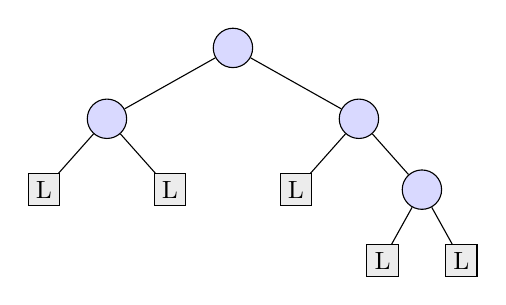
\begin{tikzpicture}[
    level distance=0.9cm,
    level 1/.style={sibling distance=3.2cm},
    level 2/.style={sibling distance=1.6cm},
    level 3/.style={sibling distance=1.0cm},
    every node/.style={font=\small},
    internal/.style={circle, draw, fill=blue!15, minimum size=5mm, inner sep=0pt},
    leaf/.style={rectangle, draw, fill=gray!15, minimum size=4mm, inner sep=1pt}
  ]
  \node[internal] {}
    child { node[internal] {}
      child { node[leaf] {L} }
      child { node[leaf] {L} }
    }
    child { node[internal] {}
      child { node[leaf] {L} }
      child { node[internal] {}
        child { node[leaf] {L} }
        child { node[leaf] {L} }
      }
    };
\end{tikzpicture}
\end{center}

Count by hand: there are 4 internal nodes (the blue circles) and 5 leaves (the gray squares), and you can trace 8 edges going down to children ($2 \times 4$, one pair per internal node). That's the pattern we're about to prove in general. The shapes $L$ stand for \texttt{Leaf} and the unmarked circles are \texttt{Node} constructors.

\subsection{Worked proof: counting edges in a binary tree}

Now let's prove something about binary trees using structural induction. We'll show that:

For all binary trees $t$:
\[
\texttt{edges}(t) = 2 \cdot \texttt{size}(t)
\]

In other words, a binary tree with $n$ internal nodes has exactly $2n$ edges (counting edges to leaf children). This makes intuitive sense: every node contributes exactly 2 edges (to its children), and leaves contribute 0.

We'll do structural induction on $t$. Our property $P(t)$ is the statement ``$\texttt{edges}(t) = 2 \cdot \texttt{size}(t)$.''

\textbf{Base case} ($t = \texttt{Leaf}$): We need $\texttt{edges(Leaf)} = 2 \cdot \texttt{size(Leaf)}$. The left side is $0$ and the right side is $2 \cdot 0 = 0$. Done.

\textbf{Inductive step} ($t = \texttt{Node(left, right)}$): Assume $P(\texttt{left})$ and $P(\texttt{right})$, i.e.\ assume:
\begin{align*}
\texttt{edges(left)} &= 2 \cdot \texttt{size(left)} && \text{(IH for left)} \\
\texttt{edges(right)} &= 2 \cdot \texttt{size(right)} && \text{(IH for right)}
\end{align*}

We need to show $\texttt{edges(Node(left, right))} = 2 \cdot \texttt{size(Node(left, right))}$.

Left side:
\begin{align*}
\texttt{edges(Node(left, right))} &= 2 + \texttt{edges(left)} + \texttt{edges(right)} && \text{(by definition of edges)} \\
&= 2 + 2 \cdot \texttt{size(left)} + 2 \cdot \texttt{size(right)} && \text{(by both IHs!)}
\end{align*}

Right side:
\begin{align*}
2 \cdot \texttt{size(Node(left, right))} &= 2 \cdot (1 + \texttt{size(left)} + \texttt{size(right)}) && \text{(by definition of size)} \\
&= 2 + 2 \cdot \texttt{size(left)} + 2 \cdot \texttt{size(right)}
\end{align*}

They're equal! Both sides give us $2 + 2 \cdot \texttt{size(left)} + 2 \cdot \texttt{size(right)}$, so $P(\texttt{Node(left, right)})$ holds. By structural induction, $P(t)$ for all binary trees $t$. $\square$

Notice how we used \textbf{both} inductive hypotheses in the inductive step---one for each subtree. That's the characteristic feature of tree induction: you get two IHs and you typically need both.

\section{The general recipe}

Let's spell out the pattern once and for all, because at this point you've seen it enough times that it should click.

Here's the recipe. Given \textbf{any} BNF definition of a datatype, you automatically get an induction principle. The correspondence is:

\begin{itemize}
  \item Each \textbf{base case} of the BNF gives you a \textbf{base case} of the proof. You need to show your property holds for each non-recursive constructor.
  \item Each \textbf{recursive case} of the BNF gives you an \textbf{inductive step}. For each recursive constructor, you get to \emph{assume} the property holds for all recursive sub-parts, and you need to \emph{show} it holds for the whole thing.
\end{itemize}

That's it. That's the whole recipe. Let's verify it against everything we've seen this quarter:

\textbf{Natural numbers:} $\texttt{Nat} := 0 \mid \texttt{succ Nat}$. One base case ($0$), one recursive case (\texttt{succ}) with one sub-part. So you get one base case and one inductive step with one IH. That's natural induction from Module 4.

\textbf{Lists:} $\texttt{List}\;A := \texttt{Nil} \mid \texttt{Cons}(A, \texttt{List}\;A)$. One base case (\texttt{Nil}), one recursive case (\texttt{Cons}) with one recursive sub-part (the tail). So you get one base case and one inductive step with one IH. Structurally identical to natural induction! And that makes sense: a list is basically a natural number that carries data.

\textbf{Binary trees:} $\texttt{BinTree} := \texttt{Leaf} \mid \texttt{Node}(\texttt{BinTree}, \texttt{BinTree})$. One base case (\texttt{Leaf}), one recursive case (\texttt{Node}) with \textbf{two} recursive sub-parts. So you get one base case and one inductive step with \textbf{two} IHs. That's the new thing we saw in this module.

And you could keep going! Imagine a datatype with two base cases and three recursive cases. You'd get two base cases and three inductive steps in your proof. Or consider propositional logic formulas from Module 2: $T$ and $F$ are base cases, ${\sim} L$ is a recursive case with one sub-part, and $L \wedge L$, $L \vee L$, $L \to L$ are recursive cases with two sub-parts each. So to prove something about all propositional formulas you'd handle the base cases ($T$, $F$, variables) and then do inductive steps for each connective, getting the appropriate number of inductive hypotheses each time.\footnote{If you go on to study programming languages or compilers, this is \emph{exactly} how you prove theorems about programs: by structural induction on the syntax of the language. The BNF of the programming language gives you the induction principle, and then you grind through the cases. It's this same recipe, just with bigger grammars.}

This extends to any datatype you can dream up---rose trees, abstract syntax trees, regular expressions, whatever. If you can write down a BNF for it, you get a structural induction principle for it. You'll see more of this in CS 251 when we work with graphs, automata, and other structures.

\subsection{Example: structural induction on propositional formulas}

Let's actually carry out that propositional-logic example instead of just waving at it. Recall the BNF from Module~2:

$L := T \mid F \mid x \mid {\sim} L \mid L \wedge L \mid L \vee L \mid L \to L$

Define a function \texttt{size} that counts the number of connectives in a formula:

\begin{lstlisting}
size(T)        = 0
size(F)        = 0
size(x)        = 0
size(~L)       = 1 + size(L)
size(L1 ^ L2)  = 1 + size(L1) + size(L2)
size(L1 v L2)  = 1 + size(L1) + size(L2)
size(L1 -> L2) = 1 + size(L1) + size(L2)
\end{lstlisting}

Seven cases, following the seven cases of the BNF---exactly the recipe we just described. Now let's prove a simple property to see the machinery work on a grammar with multiple base cases and multiple recursive cases.

\textbf{Claim.} For all formulas $f$, $\texttt{size}(f) \geq 0$.

We proceed by structural induction on $f$.

\textbf{Base cases.} If $f = T$, $f = F$, or $f = x$ (a variable), then $\texttt{size}(f) = 0 \geq 0$. Done.

\textbf{Inductive step (negation):} $f = {\sim} L$. Assume $\texttt{size}(L) \geq 0$ (IH). Then:
\begin{align*}
\texttt{size}({\sim} L) &= 1 + \texttt{size}(L) && \text{(by definition of \texttt{size})} \\
                        &\geq 1 + 0 = 1 \geq 0 && \text{(by IH)}
\end{align*}

\textbf{Inductive step (binary connectives):} $f = L_1 \star L_2$ where $\star$ is any of $\wedge$, $\vee$, $\to$. Assume $\texttt{size}(L_1) \geq 0$ (IH1) and $\texttt{size}(L_2) \geq 0$ (IH2). Then:
\begin{align*}
\texttt{size}(L_1 \star L_2) &= 1 + \texttt{size}(L_1) + \texttt{size}(L_2) && \text{(by definition of \texttt{size})} \\
                              &\geq 1 + 0 + 0 = 1 \geq 0 && \text{(by IH1 and IH2)}
\end{align*}

All cases handled. By structural induction, $\texttt{size}(f) \geq 0$ for every formula $f$. $\square$

The proof itself is almost trivially easy---and that's the point. What matters is the \emph{shape}: three base cases (matching the three non-recursive alternatives in the BNF), one inductive case with one IH (for ${\sim}$), and three inductive cases with two IHs each (for $\wedge$, $\vee$, $\to$). That shape was determined entirely by the BNF. We just followed the recipe.

\section{Wrapping up: the big picture}

Let's take a step back and look at what we've actually built over this whole course. There's been a single thread running through every module, and now we can finally state it cleanly.

The thread is a three-step pattern:
\begin{enumerate}
  \item \textbf{Define your data inductively} using BNF. Specify the base cases and the recursive cases.
  \item \textbf{Get an induction principle for free} that mirrors the structure of your definition. Base cases in the BNF become base cases in the proof. Recursive cases become inductive steps.
  \item \textbf{Use that principle to prove things} about all instances of your data by handling each case.
\end{enumerate}

We did this for propositional logic formulas in Module 2. We did this for natural numbers in Module 4. We did this for sequences in Module 8. In Module 9, we saw how \emph{strong} induction generalizes the basic induction principle to handle recurrences that reach back more than one step, and the characteristic equation technique gave us tools for solving those recurrences in closed form. And now in this module we've done it for lists and binary trees.

The specific data changes but the \emph{method} is always the same. Define inductively, get an induction principle, prove by cases. And as we saw in Module 8, this is the exact same thing as writing recursive programs: the structure of your data determines the structure of your code, which determines the structure of your proofs. Recursion, induction, and case analysis are facets of a single method depending on whether you're computing a value or proving a theorem.

If there's one thing I want you to take away from this course, it's this: when you encounter some new kind of structured data, the first question you should ask is ``what's the BNF?'' Once you have that, you know how to define functions on it (by recursion following the cases), and you know how to prove things about it (by induction following the cases). Everything else is details.

This is the foundation for CS 251 and beyond---type theory, programming language theory, algorithm analysis, formal verification. The datatypes get bigger and the proofs get harder, but the recipe stays the same. That recipe will carry you further than you might expect.\footnote{Okay, I lied a little. In CS 251 you'll see datatypes where the recursion is more complicated---mutual recursion, nested datatypes, indexed families---and the induction principles get correspondingly fancier. But the core idea really is the same. Promise.}

\section{Common mistakes}

\begin{enumerate}
  \item \textbf{Wrong number of inductive hypotheses.} The induction principle has exactly one IH per recursive sub-part in each recursive case. Students sometimes only use \emph{one} IH when proving a property of \texttt{Node(left, right)}---forgetting that they get \emph{both} $P(\texttt{left})$ and $P(\texttt{right})$. Conversely, students sometimes \emph{invent} IHs they don't have (e.g.\ claiming an IH for a parent tree when doing induction on a child). Always: IH count matches recursive-sub-part count in the BNF.
  \item \textbf{Missing a BNF case.} A structural induction proof has to handle every alternative in the BNF. If your grammar has seven alternatives (like the BNF for propositional formulas) and your proof handles five of them, you've proved a weaker statement than you think. For long grammars, explicitly list the cases at the top of the proof and check them off as you go.
  \item \textbf{Skipping the unfolding step.} The inductive step usually has the shape ``unfold the definition on the left, apply the IH, unfold the definition on the right, see they match.'' Students sometimes skip the unfolding and try to cite the IH directly on an expression where the IH doesn't actually apply---because the LHS expression has a $\texttt{Cons}$ or $\texttt{Node}$ wrapped around it and you have to \emph{unwrap} the definition first before the IH becomes applicable.
  \item \textbf{Generalizing the wrong variable.} When proving ``for all \texttt{xs} and \texttt{ys}, $\ldots$'', you usually induct on one of them with the \emph{other} universally quantified inside the predicate $P(\texttt{xs})$. If you fix a particular \texttt{ys} and then try to induct on \texttt{xs}, you might find your proof goes through---but you've only proved the result for that particular \texttt{ys}. To prove it for all \texttt{ys}, the quantifier has to be \emph{inside} $P$.
  \item \textbf{Proving a lemma you didn't state.} In the reverse-is-involution exercise (and others like it) you often need a side lemma---something like $\texttt{reverse}(xs \mathbin{++} ys) = \texttt{reverse}(ys) \mathbin{++} \texttt{reverse}(xs)$---before the main theorem can go through. Students sometimes use such a lemma mid-proof without proving it. If you need a lemma, prove it separately first (or note it and come back to it). Don't assume a useful-looking equation.
  \item \textbf{Forgetting that \texttt{Leaf} is a tree.} Base cases sometimes get short-changed because they seem trivial. But a ``trivial'' base case is still a required case; write it down explicitly and verify. The one-line base case is sometimes where the \emph{whole argument} hinges---for example, in the leaves-vs-size proof, $\texttt{leaves}(\texttt{Leaf}) = 1$ but $\texttt{size}(\texttt{Leaf}) = 0$, and you need that $0 + 1$ relationship to see why the inductive hypothesis delivers the right answer.
\end{enumerate}

\section{Summary and looking ahead}

\begin{keytakeaway}
  \item \emph{Structural induction}: every BNF definition gives you an induction principle, one case per BNF alternative, with one IH per recursive sub-part in each case.
  \item Natural induction is structural induction on $\text{Nat} := 0 \mid \text{succ Nat}$. List induction is structural induction on $\text{List} := \texttt{Nil} \mid \texttt{Cons}(A, \text{List})$. Tree induction gives you \emph{two} IHs (one per subtree). Propositional-formula induction gives you seven cases. Same recipe every time.
  \item The shape of your data determines the shape of your code (recursive functions), which determines the shape of your proofs (induction principles). Recursion, induction, and case analysis are three views of a single pattern.
  \item Serious structural induction proofs often involve \emph{lemma chains}: the main theorem depends on a helper lemma, which depends on a smaller helper, each proved by its own structural induction.
  \item Once you can name the shape of a data type, you can also name the ``right notion of sameness'' for values of that type by abstracting over some of the structure---lists up to reordering become multisets, binary trees up to relabeling become shapes, formulas up to logical equivalence become Boolean functions.
  \item That is the same move we already saw for sets (extensional equality, Module~1), formulas (logical equivalence, Module~2), and groups (isomorphism, Module~5). The intermezzo after Module~6 is the essay on the pattern.
\end{keytakeaway}

\begin{summarybox}
\textbf{What we built this module.} This is the capstone of the first term. The three-step pattern---(1) define your data inductively via BNF, (2) get an induction principle for free, (3) use it to prove things by case analysis---has been present from Module 2 (the BNF for propositional logic) through Module 4 (natural induction) to here. We've finally named it and seen it work on several concrete data types. This is the pattern that will carry you through CS 251 and beyond.

\medskip
\textbf{Looking ahead.} This is the end of the first-term notes. The intermezzi after this module (``The Algebra of Types,'' ``The Lambda Calculus'') round out the picture by showing that data types form a rich algebraic structure of their own and that there's a tiny universal programming language---$\lambda$-calculus---underneath everything we've been doing. In CS 251 you'll see mutual recursion, nested datatypes, indexed families, and eventually dependent types; the core recipe ``BNF gives you induction'' generalizes to all of it. And if you go further---into programming language theory, formal verification, or type theory---this module is the hinge on which the rest hangs.

If there's one thing to internalize from the whole first term, it's this: when you encounter some new kind of structured data, the first question to ask is ``what's the BNF?'' The answer tells you how to define functions on it and how to prove things about it. Everything else is details.
\end{summarybox}

\section{Exercises}

Organized into \textbf{warm-up} (mechanical practice with recursive definitions), \textbf{standard} (structural-induction proofs on lists and trees), \textbf{challenge} (deeper proofs, including the negation-free monotone result), and \textbf{connection} (programming and forward pointers). Solutions are in the appendix.

\subsection*{Warm-up}

\textbf{Exercise 1.}\label{ex:m10:1} Define a recursive function $\texttt{reverse}$ on lists, following the two cases of the BNF. (Hint: you will need to use \texttt{append} (\texttt{++}) in the recursive case.) Then compute $\texttt{reverse}(\texttt{Cons}(1, \texttt{Cons}(2, \texttt{Cons}(3, \texttt{Nil}))))$ step by step, showing each unfolding of the definition.

\bigskip
\textbf{Exercise 2.}\label{ex:m10:2} Compute the following by hand, unfolding the definitions step by step:
\begin{enumerate}[label=(\alph*)]
  \item $\texttt{length}(\texttt{Cons}(a, \texttt{Cons}(b, \texttt{Nil})))$
  \item $\texttt{Cons}(1, \texttt{Cons}(2, \texttt{Nil})) \mathbin{++} \texttt{Cons}(3, \texttt{Nil})$
  \item $\texttt{size}(\texttt{Node}(\texttt{Leaf}, \texttt{Node}(\texttt{Leaf}, \texttt{Leaf})))$
  \item $\texttt{edges}(\texttt{Node}(\texttt{Leaf}, \texttt{Node}(\texttt{Leaf}, \texttt{Leaf})))$
\end{enumerate}

\bigskip
\textbf{Exercise 3.}\label{ex:m10:3} For each of the following BNFs, state the shape of the structural induction principle: how many base cases and how many inductive steps, and how many IHs in each inductive step.
\begin{enumerate}[label=(\alph*)]
  \item $\texttt{Color} := \texttt{Red} \mid \texttt{Green} \mid \texttt{Blue}$
  \item $\texttt{RoseTree} := \texttt{Leaf}(A) \mid \texttt{Branch}(\texttt{List RoseTree})$ (hmm, this one is tricky because the recursive case contains a list of subtrees, not a fixed number---answer informally)
  \item $\texttt{Expr} := \texttt{Const}(\mathbb{Z}) \mid \texttt{Var}(\text{Name}) \mid \texttt{Add}(\texttt{Expr}, \texttt{Expr}) \mid \texttt{Mul}(\texttt{Expr}, \texttt{Expr}) \mid \texttt{Neg}(\texttt{Expr})$
\end{enumerate}

\subsection*{Standard}

\textbf{Exercise 4.}\label{ex:m10:4} Define a function $\texttt{leaves}(t)$ that counts the number of leaves in a binary tree (a \texttt{Leaf} counts as 1, a \texttt{Node} counts the leaves in both subtrees). Then prove by structural induction: $\texttt{leaves}(t) = \texttt{size}(t) + 1$ for all binary trees $t$. (You will need both inductive hypotheses in the inductive step, just like in the edges proof above.)

\bigskip
\textbf{Exercise 5.}\label{ex:m10:5} Define a function $\texttt{vars}(f)$ that returns the number of variable occurrences in a propositional formula (following the BNF from Module~2). For instance, $\texttt{vars}(x \wedge y) = 2$ and $\texttt{vars}(x \wedge x) = 2$ (we're counting occurrences, not distinct variables). Then prove by structural induction that for every formula $f$, $\texttt{vars}(f) \leq \texttt{size}(f) + 1$ (where $\texttt{size}$ is the connective-counting function defined in the module).

\bigskip
\textbf{Exercise 6.}\label{ex:m10:6} Prove by structural induction that append is associative on lists:
\[
  (xs \mathbin{++} ys) \mathbin{++} zs = xs \mathbin{++} (ys \mathbin{++} zs).
\]
Induct on $xs$, with $ys$ and $zs$ universally quantified inside the predicate.

\bigskip
\textbf{Exercise 7.}\label{ex:m10:7} Define $\texttt{map}(f, xs)$ recursively on lists: $\texttt{map}(f, \texttt{Nil}) = \texttt{Nil}$ and $\texttt{map}(f, \texttt{Cons}(x, xs')) = \texttt{Cons}(f(x), \texttt{map}(f, xs'))$. Prove by structural induction that $\texttt{length}(\texttt{map}(f, xs)) = \texttt{length}(xs)$ for every list $xs$.

\subsection*{Challenge}

\textbf{Exercise 8.}\label{ex:m10:8} Prove by structural induction that reverse is an involution:
\[
  \texttt{reverse}(\texttt{reverse}(xs)) = xs \quad \text{for every list } xs.
\]
You will need two helper lemmas:
\begin{enumerate}
  \item $xs \mathbin{++} \texttt{Nil} = xs$ for every $xs$. (Proof by induction on $xs$.)
  \item $\texttt{reverse}(xs \mathbin{++} ys) = \texttt{reverse}(ys) \mathbin{++} \texttt{reverse}(xs)$. (Proof by induction on $xs$, using the first lemma in the base case.)
\end{enumerate}
Prove both helpers, then use them to prove the main result. This is a good example of how real structural induction proofs often involve a chain of lemmas.

\bigskip
\textbf{Exercise 9.}\label{ex:m10:9} (The plan's request: a real semantic property.) Say a propositional formula is \emph{negation-free} if it is built from $T$, $F$, variables, and the connectives $\wedge$, $\vee$ only (i.e., the BNF excludes $\lnot$ and $\to$). Say a boolean function $f$ is \emph{monotone in variable $x$} if flipping $x$ from $F$ to $T$ (with all other variables held fixed) never flips the output of $f$ from $T$ to $F$. Prove by structural induction on the negation-free BNF:
\[
  \text{Every negation-free formula is monotone in every variable.}
\]
Hint: you'll need the sub-lemma that $\wedge$ and $\vee$ preserve monotonicity---if two functions are monotone in $x$, so is their conjunction and their disjunction. You can also look back at Module~2 Exercise~10, where you proved that $\{\wedge, \vee\}$ is not functionally complete using exactly this monotonicity idea.

\bigskip
\textbf{Exercise 10.}\label{ex:m10:10} A binary tree is \emph{perfect} if every non-leaf node has two subtrees of the same height. Define $\texttt{height}(t)$ recursively: $\texttt{height}(\texttt{Leaf}) = 0$ and $\texttt{height}(\texttt{Node}(l, r)) = 1 + \max(\texttt{height}(l), \texttt{height}(r))$. Prove by structural induction: for every perfect binary tree $t$, $\texttt{leaves}(t) = 2^{\texttt{height}(t)}$. (Hint: the definition of ``perfect'' is itself inductive: \texttt{Leaf} is perfect, and $\texttt{Node}(l, r)$ is perfect if $l$ and $r$ are both perfect and have the same height. Induct on the structure of the perfect tree.)

\subsection*{Connection}

\textbf{Exercise 11.}\label{ex:m10:11} (Programming.) Implement \texttt{List} and \texttt{BinTree} as Python classes following the BNFs. Then implement \texttt{length}, \texttt{append}, \texttt{reverse}, \texttt{size}, \texttt{edges}, \texttt{leaves}, \texttt{height} as methods or free functions. Write unit tests that check the theorems proved in the module and exercises: for instance, verify that $\texttt{length}(xs \mathbin{++} ys) = \texttt{length}(xs) + \texttt{length}(ys)$ holds on a handful of random lists. Use Python's \texttt{random} and maybe \texttt{hypothesis} (if you want a proper property-based testing library) to stress-test your implementations.

\bigskip
\textbf{Exercise 12.}\label{ex:m10:12} (Intermezzo pointer.) The ``Algebra of Types'' intermezzo that follows this module explains that BNF definitions correspond to \emph{polynomial functors}, and that the associated induction principles are cases of a general categorical theorem. As a warm-up, count the ``shape'' of each of the following datatypes by writing down a polynomial-like expression. For example, $\texttt{List}\,A := \texttt{Nil} \mid \texttt{Cons}(A, \texttt{List}\,A)$ corresponds to $L = 1 + A \cdot L$ (where $1$ stands for the \texttt{Nil} case with no data and $A \cdot L$ stands for \texttt{Cons} with an $A$ and a sub-list). Do the same for:
\begin{enumerate}[label=(\alph*)]
  \item $\texttt{Nat} := 0 \mid \texttt{succ Nat}$
  \item $\texttt{BinTree} := \texttt{Leaf} \mid \texttt{Node}(\texttt{BinTree}, \texttt{BinTree})$
  \item $\texttt{Maybe}\,A := \texttt{Nothing} \mid \texttt{Just}(A)$ (not recursive!)
\end{enumerate}
Why do you think the intermezzo calls these ``polynomial'' functors?

\end{document}


\chapter*{Intermezzo: The Algebra of Types}
\addcontentsline{toc}{chapter}{Intermezzo: The Algebra of Types}
\documentclass[11pt]{article}

\usepackage[T1]{fontenc}
\usepackage[margin=1in]{geometry}
\usepackage{amsmath, amssymb, amsthm}
\usepackage{enumitem}
\usepackage{hyperref}
\usepackage{booktabs}
\usepackage{listings}
\usepackage{xcolor}

\lstset{
  basicstyle=\ttfamily\small,
  frame=single,
  breaklines=true,
  columns=fullflexible,
  mathescape=true
}

\theoremstyle{definition}
\newtheorem{theorem}{Theorem}[section]
\newtheorem{definition}[theorem]{Definition}
\newtheorem{example}[theorem]{Example}

\title{CS 250 --- Intermezzo: The Algebra of Types}
\author{}
\date{}

\begin{document}
\maketitle

Something strange has been happening throughout this course, and it's time we talked about it.

In Module 1 we learned that $|A \times B| = |A| \cdot |B|$---the cardinality of a Cartesian product is the product of the cardinalities. In the sets intermezzo we learned that $|B^A| = |B|^{|A|}$---function spaces have exponential cardinality. And in Module 10 we defined data types using BNF, building lists and trees out of simpler pieces.

These facts live in different chapters, but they are secretly the same idea. Types obey the laws of algebra. Not metaphorically, not ``sort of''---they obey the \emph{actual} laws of high-school algebra, the ones with $+$ and $\times$ and exponents. Once you see this, a lot of things click into place.

\section{Types are like numbers}

Let's build the dictionary.

\medskip
\noindent\textbf{Product types are multiplication.} A pair $(a, b)$ where $a \in A$ and $b \in B$ has type $A \times B$. How many inhabitants does $A \times B$ have? For each choice of $a$ (there are $|A|$ many) and each choice of $b$ (there are $|B|$ many), we get a distinct pair. So $|A \times B| = |A| \cdot |B|$. A tuple is multiplication.

\medskip
\noindent\textbf{Sum types are addition.} Suppose we have a type $A + B$ that means ``either a value of type $A$, tagged with \texttt{Left}, or a value of type $B$, tagged with \texttt{Right}.'' In Haskell this is \texttt{Either A B}; in Python you might use a tagged union or a class hierarchy. How many inhabitants? Every element of $A$ gives one (tagged \texttt{Left}), and every element of $B$ gives another (tagged \texttt{Right}). So $|A + B| = |A| + |B|$. A tagged union is addition.

\medskip
\noindent\textbf{Function types are exponentiation.} A function $f : A \to B$ assigns to each element of $A$ an element of $B$. That's $|B|$ choices for each of the $|A|$ inputs, so $|A \to B| = |B|^{|A|}$. We saw this in the sets intermezzo---it's why the function space is written $B^A$. A function is exponentiation.

\medskip
\noindent\textbf{The unit type is 1.} Let $1$ denote a type with exactly one element (in Haskell, \texttt{()};  in Python, \texttt{None}). Then $A \times 1 \cong A$---a pair of an $A$ and a ``nothing'' is just an $A$, since the second component carries no information. And $1^A \cong 1$---there's only one function from $A$ to a one-element set (the function that sends everything to the single element).

\medskip
\noindent\textbf{The empty type is 0.} Let $0$ denote a type with \emph{no} elements (in Haskell, \texttt{Void}; in Python, a class you can never instantiate). Then $A \times 0 \cong 0$---you can't build a pair if the second component has no possible values. And $A + 0 \cong A$---``either an $A$ or an impossible thing'' is just an $A$. And for any nonempty $A$, $0^A \cong 0$---there are no functions from $A$ to an empty set (you'd have to send the elements of $A$ somewhere, but there's nowhere to send them).

\medskip
Look at these equations again. $A \times 1 = A$. $A + 0 = A$. $A \times 0 = 0$. Those are the rules of arithmetic you learned in grade school, but now they're facts about data types. Types form an algebra, and it's the same algebra you already know.

\section{The laws of algebra hold}

Let's verify that the familiar identities from arithmetic actually hold for types. In each case, ``$\cong$'' means ``there's a bijection between the two types''---they have the same number of inhabitants, and you can convert back and forth without losing information.

\medskip
\noindent\textbf{Multiplicative identity:} $A \times 1 \cong A$. A pair where one component is trivial is just the other component. In Haskell: \texttt{(a, ())} is isomorphic to \texttt{a}.

\medskip
\noindent\textbf{Additive identity:} $A + 0 \cong A$. \texttt{Either A Void} is isomorphic to \texttt{A}---the \texttt{Right} case is impossible (you can't construct a \texttt{Void}), so you're always in the \texttt{Left} case.

\medskip
\noindent\textbf{Distributivity:} $A \times (B + C) \cong (A \times B) + (A \times C)$. A pair of an $A$ with ``either a $B$ or a $C$'' is the same as ``either a pair of $A$ and $B$, or a pair of $A$ and $C$.'' This is the distributive law $a(b + c) = ab + ac$, in type form.

\medskip
\noindent\textbf{Exponent of a product:} $A \to (B \times C) \cong (A \to B) \times (A \to C)$. A function that returns a pair is the same as a pair of functions. If I ask you for a machine that takes an input and produces two outputs, you can either build one machine with two output slots or build two separate machines---same thing.

\medskip
\noindent\textbf{Exponent of a sum:} $(A + B) \to C \cong (A \to C) \times (B \to C)$. A function from ``either an $A$ or a $B$'' is the same as a pair of functions: one that handles $A$ inputs and one that handles $B$ inputs. In Python:

\begin{lstlisting}[language=Python]
# A function from Either is a pair of handlers:
def handle_either(x):
    if isinstance(x, Left):
        return handle_a(x.value)   # the A -> C part
    else:
        return handle_b(x.value)   # the B -> C part
\end{lstlisting}

Wait a moment. A function from a sum is a pair of handlers---one for each case. Isn't that exactly \emph{proof by cases}? In Module 3 we learned the disjunction elimination rule: if you want to prove something from $A \vee B$, you handle the $A$ case and handle the $B$ case separately. That's the logical version of $(A + B) \to C \cong (A \to C) \times (B \to C)$---or-elimination \emph{is} the fact that a function from a sum is a pair of functions. The algebra is telling us something about logic.

\section{Data types as polynomials}

Here is where things get a little bit magical.

In Module 10 we defined lists with a BNF:

\begin{lstlisting}
List A := Nil | Cons(A, List A)
\end{lstlisting}

In our algebraic notation, \texttt{Nil} is the unit type $1$ (one way to be empty) and \texttt{Cons(A, List A)} is a product $A \times L$ where $L$ is the type of lists. The \texttt{|} in the BNF is a sum. So the definition of lists is:
\[
L = 1 + A \cdot L
\]

That's a polynomial equation! Let's be reckless and solve it like one. Rearranging:
\[
L - A \cdot L = 1 \qquad \Longrightarrow \qquad L(1 - A) = 1 \qquad \Longrightarrow \qquad L = \frac{1}{1 - A}
\]

Now, you might be having a reasonable objection right now, which is: what does it even \emph{mean} to divide types or subtract types? Fair enough. But let's push ahead and see what happens. From Module 9, we know the formula for a geometric series:
\[
\frac{1}{1 - x} = 1 + x + x^2 + x^3 + \cdots
\]

So if we just blindly expand:
\[
L = 1 + A + A^2 + A^3 + A^4 + \cdots
\]

And what is this saying? A list of $A$'s is:
\begin{itemize}
  \item $1$: the empty list (one way), or
  \item $A$: a single element (one $A$), or
  \item $A^2 = A \times A$: two elements (a pair of $A$'s), or
  \item $A^3 = A \times A \times A$: three elements, or
  \item $\ldots$and so on forever.
\end{itemize}

That's \emph{exactly right}. A list is either empty, or has one element, or has two, or three, or any finite number of elements. The algebra of types---this insane-looking manipulation where we divided by $(1 - A)$ as if types were numbers---told us the truth. The geometric series from Module 9 is secretly a statement about data structures.

\medskip
Let's try another one. Binary trees from Module 10 were defined as:

\begin{lstlisting}
Tree := Leaf | Node(Tree, Tree)
\end{lstlisting}

In algebraic notation:
\[
T = 1 + T^2
\]

This is a quadratic equation! Rearranging: $T^2 - T + 1 = 0$, and the quadratic formula gives
\[
T = \frac{1 \pm \sqrt{1 - 4}}{2} = \frac{1 \pm \sqrt{-3}}{2}
\]

which involves complex numbers and seems completely unhinged. But remarkably, if you take the right root and expand it as a power series, you get the \emph{Catalan numbers}---which are exactly the number of distinct binary trees with $n$ internal nodes. The algebra of types knows about combinatorics.

We won't push this further here, but the point is: these aren't parlor tricks. There is a rigorous mathematical theory---the theory of \emph{combinatorial species}---that makes all of this precise. The equation $L = 1 + A \cdot L$ is a legitimate algebraic equation in that theory, the ``division'' is a real operation, and the geometric series expansion is a theorem, not a coincidence.

What we're seeing is a remarkable convergence: the sets intermezzo (cardinality of function spaces), Module 9 (geometric series), and Module 10 (BNF definitions of data types) are all aspects of a single algebraic framework. Types are numbers, data definitions are polynomial equations, and the power series you learned in Module 9 enumerate the shapes of data structures.

\section{The Curry--Howard connection}

There's one more layer. In the Curry--Howard intermezzo we learned that types correspond to propositions: a type is ``true'' if it's inhabited (has at least one value) and ``false'' if it's empty. Under this correspondence:

\begin{center}
\begin{tabular}{lll}
\toprule
\textbf{Algebra} & \textbf{Types} & \textbf{Logic} \\
\midrule
$A \cdot B$ & $A \times B$ (product) & $A \wedge B$ (conjunction) \\
$A + B$ & $A + B$ (sum) & $A \vee B$ (disjunction) \\
$B^A$ & $A \to B$ (function) & $A \to B$ (implication) \\
$1$ & Unit & $\top$ (true) \\
$0$ & Void & $\bot$ (false) \\
\bottomrule
\end{tabular}
\end{center}

So the algebraic identities we verified in Section 2 are also \emph{logical tautologies}:
\begin{itemize}
  \item $A \times 1 \cong A$ is $A \wedge \top \equiv A$ (``$A$ and true'' is just $A$)
  \item $A + 0 \cong A$ is $A \vee \bot \equiv A$ (``$A$ or false'' is just $A$)
  \item $A \times (B + C) \cong (A \times B) + (A \times C)$ is the distribution of $\wedge$ over $\vee$
  \item $(A + B) \to C \cong (A \to C) \times (B \to C)$ is or-elimination
  \item $A \times 0 \cong 0$ is $A \wedge \bot \equiv \bot$ (``$A$ and false'' is false)
\end{itemize}

Three parallel worlds---arithmetic, type theory, and logic---and they're all obeying the same laws. The algebra of numbers, the algebra of types, and the algebra of propositions are three views of one structure.

That structure has a name, by the way. It's called a \emph{rig}\index{rig} (a ``ring without negation''---because you can't subtract types or negate propositions in general). But you don't need to know the name to appreciate the fact: the math you already know, from all across this course, fits together like a puzzle. Cardinality is counting. Types are numbers. BNF definitions are polynomial equations. Proofs are programs. And the geometric series from Module 9 secretly counts the shapes of lists.

\section{Exercises}

\bigskip
\textbf{Exercise 1.}\label{ex:ta:1} Using the algebra of types, simplify the type $(A \to B) \times (A \to C)$. What single type is it isomorphic to? What does this isomorphism correspond to as a logical proposition (under the Curry--Howard correspondence)?

\bigskip
\textbf{Exercise 2.}\label{ex:ta:2} The BNF for natural numbers is \texttt{Nat = Zero | Succ(Nat)}, which in our algebraic notation is $N = 1 + N$. Write this as a ``polynomial equation'' and ``solve'' for $N$ by expanding as a series. Does the series $1 + 1 + 1 + 1 + \cdots$ make sense as a description of the natural numbers? (Hint: what does $1^n = 1$ mean for the $n$th term?)

\bigskip
\textbf{Exercise 3.}\label{ex:ta:3} (Distributivity, programmatically.) Use the algebra of types to simplify $(A + B) \times (C + D)$. What single ``polynomial'' do you get? Convert your answer back into a Python data structure: write a class hierarchy or tagged union with one constructor for each summand of the result. What logical tautology does this correspond to under Curry--Howard?

\bigskip
\textbf{Exercise 4.}\label{ex:ta:4} (Solving for non-empty lists.) Define non-empty lists by the BNF
\[
  \texttt{NEList A} = A \;\mid\; A \times \texttt{NEList A}
\]
that is, ``either a single $A$, or an $A$ followed by a non-empty list of $A$.'' Translate this to a polynomial equation in $L$ (where $L = \texttt{NEList A}$), solve for $L$ algebraically, and expand the result as a series. What kinds of values appear in the series, and how does that match the structure of a non-empty list?

\bigskip
\textbf{Exercise 5.}\label{ex:ta:5} (The \texttt{Maybe} type.) The type \texttt{Maybe A} (in Haskell) is defined as \texttt{Just A | Nothing}. In algebraic notation: $\texttt{Maybe } A = A + 1$.
\begin{enumerate}[label=(\alph*)]
  \item What is $|\texttt{Maybe } A|$ in terms of $|A|$?
  \item What is $|\texttt{Maybe (Maybe } A\texttt{)}|$ in terms of $|A|$?
  \item Express \texttt{Maybe (Maybe A)} as an algebraic expression and simplify. Why does the answer match the cardinality formula in (b)?
\end{enumerate}

\bigskip
\textbf{Exercise 6.}\label{ex:ta:6} (A function that returns a pair is a pair of functions.) Verify the isomorphism
\[
  A \to (B \times C) \;\cong\; (A \to B) \times (A \to C)
\]
by writing two Python functions: one that converts the left side into the right side, and one that converts the right side into the left side. Verify (informally, by trying out a few examples) that they are inverses of each other. What does this say in pure-arithmetic terms about the equation $(b \cdot c)^a = b^a \cdot c^a$?

\section*{Further reading}

If the algebra of types appeals to you, here is where to go next. The connection to combinatorics is deep and beautiful.

\begin{itemize}
  \item Conor McBride, ``The Derivative of a Regular Type is its Type of One-Hole Contexts,'' unpublished manuscript (2001), available on the author's homepage at \texttt{strictlypositive.org}. A short, witty, surprisingly elementary derivation of why \emph{differentiating} an algebraic data type literally gives you its zipper. Connects high-school calculus to programming in a way undergraduates love.
  \item Brent Yorgey, ``Species and Functors and Types, Oh My!'' \emph{Haskell Symposium 2010}. Written explicitly as an accessible bridge between Joyal's combinatorial species and the algebraic data types programmers already know. The most undergraduate-friendly entry point to species I know of.
  \item Philippe Flajolet and Robert Sedgewick, \emph{\href{https://ac.cs.princeton.edu/home/}{Analytic Combinatorics}}, Cambridge University Press (2009), Chapter I (``Symbolic Methods''). The full book PDF is freely available on Sedgewick's Princeton homepage. Chapter I introduces the symbolic method---sums, products, sequences as type combinators with generating functions---at exactly the level a strong undergrad can handle.
\end{itemize}

\end{document}


\chapter*{Intermezzo: The Lambda Calculus}
\addcontentsline{toc}{chapter}{Intermezzo: The Lambda Calculus}
\documentclass[11pt]{article}

\usepackage[T1]{fontenc}
\usepackage[margin=1in]{geometry}
\usepackage{amsmath, amssymb, amsthm}
\usepackage{enumitem}
\usepackage{hyperref}
\usepackage{booktabs}
\usepackage{listings}
\usepackage{xcolor}

\lstset{
  basicstyle=\ttfamily\small,
  frame=single,
  breaklines=true,
  columns=fullflexible,
  mathescape=true
}

\theoremstyle{definition}
\newtheorem{theorem}{Theorem}[section]
\newtheorem{definition}[theorem]{Definition}
\newtheorem{example}[theorem]{Example}

\title{CS 250 --- Intermezzo: The Lambda Calculus}
\author{}
\date{}

\begin{document}
\maketitle

We've reached the end of CS 250. Over the past ten modules you've learned how to define data with BNF, how to prove things about data with induction, and---in the intermezzi on Curry--Howard and the algebra of types---how proofs and programs are secretly the same thing. But there's a question we left hanging all the way back in Module 1 that I want to come back to now.

Remember the question? We asked: if we want to understand what computers can do \emph{ever}---not just what today's chips can handle---we need an abstract model of computation, one that doesn't depend on hardware or programming language. We said we'd leave the answer for CS 251. But we can give a preview now, and it turns out that almost everything you need to understand the answer has been hiding in this course the whole time.

\section{A mathematical model of computation}

In the 1930s, before electronic computers existed, a mathematician named Alonzo Church\index{Church, Alonzo} asked a foundational question: what does it mean to \emph{compute} something? His answer was the \textbf{lambda calculus}\index{lambda calculus}---the simplest possible programming language. Not a practical language you'd use to build a web app, but a theoretical one, stripped down to the absolute minimum needed to express any computation at all.

How minimal? The entire language has exactly three constructs. Here's the BNF\@:
\[
M \;:=\; x \;\mid\; \lambda x.\; M \;\mid\; M\; M
\]

That's it. Three things:
\begin{itemize}
  \item \textbf{Variables} ($x$): names that stand for values. You've seen these since Module 2.
  \item \textbf{Abstraction} ($\lambda x.\; M$): a function definition. The $\lambda$ says ``I'm defining a function whose parameter is $x$ and whose body is $M$.'' If you've written \texttt{def f(x): return M} in Python or \texttt{fun x -> M} in OCaml, you already know what this is. The $\lambda$ is just the world's oldest anonymous function syntax.
  \item \textbf{Application} ($M\; M$): a function call. Put a function next to its argument and it runs.
\end{itemize}

No numbers. No booleans. No if-statements. No loops. No data structures. Just variables, function definitions, and function calls. You're probably thinking: how can you compute \emph{anything} with that? The answer is one of the most surprising facts in all of computer science. You can build everything from functions alone.

\section{Computing with pure functions}

The lambda calculus has one rule of computation, called \textbf{beta reduction}\index{beta reduction}. It says: when you apply a function to an argument, substitute the argument for the parameter in the body. In symbols:
\[
(\lambda x.\; M)\; N \;\longrightarrow\; M[N/x]
\]
where $M[N/x]$ means ``$M$ with every occurrence of $x$ replaced by $N$.'' That's it. That's the entire execution model.

\begin{example}[The identity function]
The term $\lambda x.\; x$ is a function that takes its argument and returns it unchanged. Apply it to 5:
\[
(\lambda x.\; x)\; 5 \;\longrightarrow\; x[5/x] \;=\; 5
\]
The identity function applied to 5 gives 5. Not very exciting, but it illustrates the rule.
\end{example}

\begin{example}[Applying a function twice]
Consider the term $\lambda f.\; \lambda x.\; f\;(f\; x)$. This takes a function $f$ and a value $x$, and applies $f$ twice. If $f$ is ``add 1'' and $x$ is $0$:
\begin{align*}
(\lambda f.\; \lambda x.\; f\;(f\; x))\;\text{add1}\; 0
  &\;\longrightarrow\; (\lambda x.\; \text{add1}\;(\text{add1}\; x))\; 0 \\
  &\;\longrightarrow\; \text{add1}\;(\text{add1}\; 0) \\
  &\;=\; \text{add1}\; 1 \\
  &\;=\; 2
\end{align*}
Does this remind you of anything? In Module 4, we defined the natural numbers with a successor function $\text{succ}$ and a base case $0$. Applying $\text{succ}$ twice to $0$ gives $2$. The idea of ``iterate a function $n$ times'' is about to become very important.
\end{example}

Notice something familiar about the BNF for lambda terms. It has a recursive structure: the body of an abstraction is itself a lambda term, and both parts of an application are lambda terms. By the pattern from Module 10, this BNF gives us a principle of \emph{structural induction on lambda terms}\index{structural induction!on lambda terms}---three cases, one for each construct. This is exactly how programming language theorists prove properties of languages: by induction on the syntax. The tools you learned in Module 10 are the same tools the researchers use.

\section{Church encodings---building everything from nothing}

Here is where things get genuinely mind-bending. Since the lambda calculus has no built-in data types, Church figured out how to \emph{encode} data as functions. The strategy is elegant: represent a piece of data by what you can \emph{do with it}.

\subsection*{Church booleans}

What can you do with a boolean? You use it to choose between two alternatives. So let's define booleans as choosers:
\begin{align*}
\text{true}  &= \lambda t.\; \lambda f.\; t  && \text{(given two options, pick the first)} \\
\text{false} &= \lambda t.\; \lambda f.\; f  && \text{(given two options, pick the second)}
\end{align*}

A boolean \emph{is} an if-statement. Given two branches, it picks one. In fact, the ``if'' function is almost trivial:
\[
\text{if} = \lambda b.\; \lambda t.\; \lambda f.\; b\; t\; f
\]
It just hands the two branches to the boolean and lets the boolean decide. Let's verify:
\[
\text{if}\;\text{true}\;a\;b \;\longrightarrow\; \text{true}\;a\;b \;\longrightarrow\; (\lambda t.\;\lambda f.\; t)\;a\;b \;\longrightarrow\; (\lambda f.\; a)\;b \;\longrightarrow\; a
\]
It works. And this connects directly to Module 2: we're encoding T and F---the truth values of propositional logic---as pure functions. The logical constants have become computational objects.

\subsection*{Church numerals}

What can you do with a natural number $n$? You can use it to \emph{repeat} something $n$ times. So let's define a natural number as a function that iterates its argument:
\begin{align*}
\mathbf{0} &= \lambda f.\; \lambda x.\; x              && \text{(apply $f$ zero times)} \\
\mathbf{1} &= \lambda f.\; \lambda x.\; f\; x           && \text{(apply $f$ once)} \\
\mathbf{2} &= \lambda f.\; \lambda x.\; f\;(f\; x)      && \text{(apply $f$ twice)} \\
\mathbf{3} &= \lambda f.\; \lambda x.\; f\;(f\;(f\; x)) && \text{(apply $f$ three times)} \\
    &\;\;\vdots \\
\mathbf{n} &= \lambda f.\; \lambda x.\; f^n\; x          && \text{(apply $f$ $n$ times)}
\end{align*}

Stop and look at this. A Church numeral $\mathbf{n}$ takes a function $f$ and a starting value $x$, and applies $f$ to $x$ exactly $n$ times. Zero applies $f$ zero times (just returns $x$). One applies $f$ once. And so on.

Now here's the connection I want you to see. In Module 4 we defined the natural numbers by BNF:

\begin{lstlisting}
Nat := 0 | succ(Nat)
\end{lstlisting}

Two cases: a base case ($0$) and a recursive case (apply $\text{succ}$ one more time). Church numerals are \emph{the same definition in disguise}. The base case is $x$ (the ``zero'' of the iteration). The recursive case is ``apply $f$ one more time.'' Church numeral $\mathbf{n}$ is literally $\text{succ}^n(0)$ with $\text{succ}$ renamed to $f$ and $0$ renamed to $x$. The BNF and the Church encoding are two faces of the same coin.

With this insight, the successor function writes itself:
\[
\text{succ} = \lambda n.\; \lambda f.\; \lambda x.\; f\;(n\; f\; x)
\]
Given a Church numeral $n$, this produces a new numeral that applies $f$ one extra time: $n$ already applies $f$ $n$ times to $x$, and then we wrap one more $f$ around the result. That's ``apply $f$ one more time''---exactly the recursive case of the BNF\@.

And addition? Apply $f$ a total of $m + n$ times by first applying it $n$ times, then $m$ more:
\[
\text{add} = \lambda m.\; \lambda n.\; \lambda f.\; \lambda x.\; m\; f\;(n\; f\; x)
\]
The term $n\; f\; x$ applies $f$ $n$ times to $x$. Then $m\; f$ applies $f$ $m$ more times to that result. Total: $m + n$ applications.

\section{Why this matters}

We started this course by asking whether Python and C can solve the same problems, and whether some future computer might solve problems that today's computers can't. The lambda calculus gives us the tools to answer these questions.

\textbf{The Church--Turing thesis.}\index{Church--Turing thesis} In the same decade that Church invented the lambda calculus, Alan Turing independently invented a different model of computation---the Turing machine, a kind of abstract tape-reading automaton. The two models look nothing alike. But Church and Turing proved that they compute exactly the same class of functions. Every function computable by a Turing machine can be computed in the lambda calculus, and vice versa. This result has been replicated for every ``reasonable'' model of computation anyone has ever proposed: register machines, cellular automata, Post systems, RAM machines, quantum computers. They all compute the same things. The \textbf{Church--Turing thesis} is the claim that this class---the class of functions computable by any of these models---is \emph{the} right notion of ``computable.''

This is the answer to Module 1's question. Python and C can solve the same problems because they are both models of computation at least as powerful as the lambda calculus (and no more powerful). No future chip will change this. The limits of computation are not engineering constraints---they are mathematical facts, and the lambda calculus is one of the cleanest ways to see them.

\textbf{The lambda calculus is the ancestor of every functional language.} Haskell, ML, OCaml, Lisp, Scheme, Clojure, Erlang, F\#---all of them are, at their core, the lambda calculus with syntactic sugar on top. When you write a lambda expression in Python (\texttt{lambda x: x + 1}), you are writing a Church-style abstraction. The notation is literally named after Church's $\lambda$.

\textbf{Under Curry--Howard, lambda terms are proofs.} In the previous intermezzo, we saw that proofs correspond to programs and propositions correspond to types. The programs in that correspondence are lambda terms. So the simplest possible model of computation is also the simplest possible language of mathematical proof. A lambda term of type $A \to B$ is simultaneously a function from $A$ to $B$ and a proof that $A$ implies $B$. Defining a function \emph{is} introducing an implication. Applying a function \emph{is} modus ponens. The act of computing and the act of reasoning are, at bottom, the same act.

\textbf{BNF, induction, Curry--Howard, and the lambda calculus form a single story.} The BNF for lambda terms ($M := x \mid \lambda x.\; M \mid M\; M$) gives you structural induction on terms. Structural induction lets you prove properties of programs. Curry--Howard tells you those programs are proofs. And the Church--Turing thesis tells you those programs capture all of computation. The entire course---from the first BNF in Module 2 to the structural induction of Module 10, from the proof rules of Module 3 to the Curry--Howard correspondence---was building toward this point. Logic, proof, computation, and data are not four separate subjects. They are four views of one subject. CS 251 will make that precise.

\section{Exercises}

\bigskip
\textbf{Exercise 1.}\label{ex:lambda:1} Evaluate $(\lambda x.\; \lambda y.\; x)\; 3\; 7$ by applying beta reduction step by step. What does this function do? (Hint: the expression $(\lambda x.\; \lambda y.\; x)\; 3\; 7$ means $((\lambda x.\; \lambda y.\; x)\; 3)\; 7$---application is left-associative.)

\bigskip
\textbf{Exercise 2.}\label{ex:lambda:2} Write a Church encoding for the boolean operation AND\@. Hint: $\text{and} = \lambda a.\; \lambda b.\; a\; b\; \text{false}$. Verify that this definition is correct by evaluating it on all four input combinations: $\text{and}\;\text{true}\;\text{true}$, $\text{and}\;\text{true}\;\text{false}$, $\text{and}\;\text{false}\;\text{true}$, and $\text{and}\;\text{false}\;\text{false}$. For each case, show the beta reduction steps and confirm the result matches the expected truth value.

\end{document}


\appendix
\chapter{Notation Summary}
\documentclass[11pt]{article}

% cs250preamble.tex --- shared preamble for CS 250 course notes
%
% This file is \input by main.tex and by each individual module
% file so that each module can still compile standalone. Any
% package or custom-environment change should be made here, not
% in the individual module files.

\usepackage[T1]{fontenc}
\usepackage[margin=1in]{geometry}
\usepackage{amsmath, amssymb, amsthm}
\usepackage{enumitem}
\usepackage{hyperref}
\usepackage{booktabs}
\usepackage{listings}
\usepackage{xcolor}
\usepackage{tikz}
\usetikzlibrary{shapes.geometric, shapes.gates.logic.US, shapes.gates.logic.IEC, arrows.meta, positioning, calc, trees}
\usepackage{bussproofs}
\usepackage{mdframed}

\lstset{
  basicstyle=\ttfamily\small,
  frame=single,
  breaklines=true,
  columns=fullflexible,
  mathescape=true
}

\theoremstyle{definition}
\newtheorem{theorem}{Theorem}[section]
\newtheorem{definition}[theorem]{Definition}
\newtheorem{example}[theorem]{Example}

\hypersetup{
  colorlinks=true,
  linkcolor=blue!60!black,
  urlcolor=blue!60!black
}

% Key-takeaway box: used at the end of major sections and at the end of
% each module to summarise the main points. Expects \item bullets inside.
\newmdenv[
  linewidth=0.8pt,
  linecolor=blue!40!black,
  backgroundcolor=blue!3,
  skipabove=8pt,
  skipbelow=8pt,
  innertopmargin=7pt,
  innerbottommargin=7pt,
  innerleftmargin=9pt,
  innerrightmargin=9pt
]{keytakeawaybox}
\newenvironment{keytakeaway}{%
  \begin{keytakeawaybox}%
  \noindent\textbf{Key takeaways.}%
  \begin{itemize}[leftmargin=1.3em, topsep=2pt, itemsep=1pt, label=\textbullet]%
}{%
  \end{itemize}%
  \end{keytakeawaybox}%
}

% Summary/looking-ahead environment: used once at the end of each module
% to wrap up what the module built and point forward.
\newmdenv[
  linewidth=0.8pt,
  linecolor=gray!60,
  backgroundcolor=gray!5,
  skipabove=8pt,
  skipbelow=8pt,
  innertopmargin=7pt,
  innerbottommargin=7pt,
  innerleftmargin=9pt,
  innerrightmargin=9pt
]{summarybox}

% Sidebar environment: used for tangential asides---historical notes,
% pointers to other areas of math/CS, cross-paradigm remarks---that
% enrich the main narrative without being essential to it. Takes one
% argument: the sidebar's title.
\newmdenv[
  linewidth=0.6pt,
  linecolor=gray!60,
  backgroundcolor=gray!4,
  skipabove=8pt,
  skipbelow=8pt,
  innertopmargin=6pt,
  innerbottommargin=6pt,
  innerleftmargin=9pt,
  innerrightmargin=9pt
]{sidebarbox}
\newenvironment{sidebar}[1]{%
  \begin{sidebarbox}%
  \noindent\textbf{Sidebar: #1.}\par\medskip%
}{%
  \end{sidebarbox}%
}

% Reading-map environment: used at the top of each numbered module to
% indicate Epp coverage, prerequisites, relevant intermezzi, and
% suggested practice problems. Expects four \rmentry{label}{body}
% items inside (or arbitrary paragraphs).
\newmdenv[
  linewidth=0.8pt,
  linecolor=black!55,
  backgroundcolor=yellow!4,
  skipabove=10pt,
  skipbelow=14pt,
  innertopmargin=9pt,
  innerbottommargin=9pt,
  innerleftmargin=11pt,
  innerrightmargin=11pt
]{readingmapbox}
\newcommand{\rmentry}[2]{\par\noindent\textbf{#1}\hspace{0.4em}#2\par}
\newenvironment{readingmap}{%
  \begin{readingmapbox}%
  \noindent{\bfseries\large Reading map}%
  \vspace{2pt}%
  \setlength{\parskip}{4pt plus 1pt}%
}{%
  \end{readingmapbox}%
}


\title{CS 250 --- Notation Summary}
\author{}
\date{}

\begin{document}
\maketitle

{\small
\begin{center}
\begin{tabular}{lll}
\toprule
\textbf{Symbol} & \textbf{Name} & \textbf{Introduced in} \\
\midrule
\multicolumn{3}{l}{\textit{Propositional Logic}} \\[2pt]
$\wedge$ & Conjunction (and) & Module 2 \\
$\vee$ & Disjunction (or) & Module 2 \\
$\lnot$ or $\sim$ & Negation (not) & Module 2 \\
$\to$ & Implication (if\ldots then) & Module 2 \\
$\leftrightarrow$ & Biconditional (if and only if) & Module 2 \\
$\equiv$ & Logical equivalence & Module 2 \\
$\oplus$ & Exclusive or (XOR) & Module 2 \\
T, F & Truth values & Module 2 \\
$\bot$ & Absurdity / falsum & Gentzen Intermezzo \\
\midrule
\multicolumn{3}{l}{\textit{Quantifiers and Predicates}} \\[2pt]
$\forall$ & For all (universal quantifier) & Module 4 \\
$\exists$ & There exists (existential quantifier) & Module 4 \\
$P(x)$ & Predicate applied to $x$ & Module 4 \\
\midrule
\multicolumn{3}{l}{\textit{Sets}} \\[2pt]
$\{\ \}$ & Set braces & Module 1 \\
$\in$, $\notin$ & Element of, not element of & Module 1 \\
$\subseteq$ & Subset & Module 1 \\
$\cap$ & Intersection & Module 1 \\
$\cup$ & Union & Module 1 \\
$\setminus$ & Set difference & Module 1 \\
$\overline{A}$ & Complement & Module 1 \\
$\emptyset$ & Empty set & Module 1 \\
$|A|$ & Cardinality & Module 1 \\
$\mathcal{P}(A)$ & Power set & Module 1 \\
$A \times B$ & Cartesian product & Module 1 \\
$B^A$ & Function space ($A \to B$) & Cardinality Intermezzo \\
$\{x \mid P(x)\}$ & Set-builder notation & Module 1 \\
\midrule
\multicolumn{3}{l}{\textit{Functions and Relations}} \\[2pt]
$f : A \to B$ & Function from $A$ to $B$ & Module 1 \\
$a\, R\, b$ & $a$ is related to $b$ by $R$ & Module 1 \\
$\cong$ & Isomorphism / bijection exists & Cardinality Intermezzo \\
\bottomrule
\end{tabular}
\end{center}
}

\clearpage

{\small
\begin{center}
\begin{tabular}{lll}
\toprule
\textbf{Symbol} & \textbf{Name} & \textbf{Introduced in} \\
\midrule
\multicolumn{3}{l}{\textit{Number Theory}} \\[2pt]
$\mathbb{N}$ & Natural numbers & Module 1 \\
$\mathbb{Z}$ & Integers & Module 5 \\
$\mathbb{Q}$ & Rationals & Module 5 \\
$\mathbb{R}$ & Reals & Module 4 \\
$a \mid b$ & $a$ divides $b$ & Module 5 \\
$\gcd(a,b)$ & Greatest common divisor & Module 7 \\
$\mathbb{Z}/n\mathbb{Z}$ & Integers mod $n$ & Module 6 \\
$\lfloor x \rfloor$, $\lceil x \rceil$ & Floor, ceiling & Module 6 \\
\midrule
\multicolumn{3}{l}{\textit{Sequences and Sums}} \\[2pt]
$a_n$ & $n$th term of a sequence & Module 8 \\
$\sum$ & Summation & Module 8 \\
$\prod$ & Product & Module 8 \\
$n!$ & Factorial & Module 8 \\
\midrule
\multicolumn{3}{l}{\textit{Data Structures}} \\[2pt]
Nil, Cons & List constructors & Module 10 \\
Leaf, Node & Binary tree constructors & Module 10 \\
\midrule
\multicolumn{3}{l}{\textit{Proof Notation}} \\[2pt]
$\therefore$ & Therefore & Module 3 \\
$\square$ or QED & End of proof & Throughout \\
$\{P\}\,C\,\{Q\}$ & Hoare triple & Module 7 \\
\bottomrule
\end{tabular}
\end{center}
}

\end{document}


\chapter{Solutions to Exercises}
\documentclass[11pt]{article}

% cs250preamble.tex --- shared preamble for CS 250 course notes
%
% This file is \input by main.tex and by each individual module
% file so that each module can still compile standalone. Any
% package or custom-environment change should be made here, not
% in the individual module files.

\usepackage[T1]{fontenc}
\usepackage[margin=1in]{geometry}
\usepackage{amsmath, amssymb, amsthm}
\usepackage{enumitem}
\usepackage{hyperref}
\usepackage{booktabs}
\usepackage{listings}
\usepackage{xcolor}
\usepackage{tikz}
\usetikzlibrary{shapes.geometric, shapes.gates.logic.US, shapes.gates.logic.IEC, arrows.meta, positioning, calc, trees}
\usepackage{bussproofs}
\usepackage{mdframed}

\lstset{
  basicstyle=\ttfamily\small,
  frame=single,
  breaklines=true,
  columns=fullflexible,
  mathescape=true
}

\theoremstyle{definition}
\newtheorem{theorem}{Theorem}[section]
\newtheorem{definition}[theorem]{Definition}
\newtheorem{example}[theorem]{Example}

\hypersetup{
  colorlinks=true,
  linkcolor=blue!60!black,
  urlcolor=blue!60!black
}

% Key-takeaway box: used at the end of major sections and at the end of
% each module to summarise the main points. Expects \item bullets inside.
\newmdenv[
  linewidth=0.8pt,
  linecolor=blue!40!black,
  backgroundcolor=blue!3,
  skipabove=8pt,
  skipbelow=8pt,
  innertopmargin=7pt,
  innerbottommargin=7pt,
  innerleftmargin=9pt,
  innerrightmargin=9pt
]{keytakeawaybox}
\newenvironment{keytakeaway}{%
  \begin{keytakeawaybox}%
  \noindent\textbf{Key takeaways.}%
  \begin{itemize}[leftmargin=1.3em, topsep=2pt, itemsep=1pt, label=\textbullet]%
}{%
  \end{itemize}%
  \end{keytakeawaybox}%
}

% Summary/looking-ahead environment: used once at the end of each module
% to wrap up what the module built and point forward.
\newmdenv[
  linewidth=0.8pt,
  linecolor=gray!60,
  backgroundcolor=gray!5,
  skipabove=8pt,
  skipbelow=8pt,
  innertopmargin=7pt,
  innerbottommargin=7pt,
  innerleftmargin=9pt,
  innerrightmargin=9pt
]{summarybox}

% Sidebar environment: used for tangential asides---historical notes,
% pointers to other areas of math/CS, cross-paradigm remarks---that
% enrich the main narrative without being essential to it. Takes one
% argument: the sidebar's title.
\newmdenv[
  linewidth=0.6pt,
  linecolor=gray!60,
  backgroundcolor=gray!4,
  skipabove=8pt,
  skipbelow=8pt,
  innertopmargin=6pt,
  innerbottommargin=6pt,
  innerleftmargin=9pt,
  innerrightmargin=9pt
]{sidebarbox}
\newenvironment{sidebar}[1]{%
  \begin{sidebarbox}%
  \noindent\textbf{Sidebar: #1.}\par\medskip%
}{%
  \end{sidebarbox}%
}

% Reading-map environment: used at the top of each numbered module to
% indicate Epp coverage, prerequisites, relevant intermezzi, and
% suggested practice problems. Expects four \rmentry{label}{body}
% items inside (or arbitrary paragraphs).
\newmdenv[
  linewidth=0.8pt,
  linecolor=black!55,
  backgroundcolor=yellow!4,
  skipabove=10pt,
  skipbelow=14pt,
  innertopmargin=9pt,
  innerbottommargin=9pt,
  innerleftmargin=11pt,
  innerrightmargin=11pt
]{readingmapbox}
\newcommand{\rmentry}[2]{\par\noindent\textbf{#1}\hspace{0.4em}#2\par}
\newenvironment{readingmap}{%
  \begin{readingmapbox}%
  \noindent{\bfseries\large Reading map}%
  \vspace{2pt}%
  \setlength{\parskip}{4pt plus 1pt}%
}{%
  \end{readingmapbox}%
}


\title{CS 250 --- Solutions to Exercises}
\author{}
\date{}

\begin{document}
\maketitle

%% ---------- Module 1 ----------
\section*{Module 1}

\subsection*{Warm-up}

\textbf{Exercise 1.}
Let $A = \{1,2,3,4\}$ and $B = \{3,4,5,6\}$.
\begin{align*}
  A \cap B &= \{3, 4\}, \\
  A \cup B &= \{1, 2, 3, 4, 5, 6\}, \\
  A \setminus B &= \{1, 2\}, \\
  |A \times B| &= |A| \cdot |B| = 4 \times 4 = 16.
\end{align*}

\medskip
\textbf{Exercise 2.}
The set $\{1,\;\{1\},\;\{1,\{1\}\}\}$ has three distinct elements: $1$,
$\{1\}$, and $\{1,\{1\}\}$.  Therefore
$|\{1,\;\{1\},\;\{1,\{1\}\}\}| = 3$.

\medskip
\textbf{Exercise 3.}
For the first set, we want natural numbers $n$ with $n^2 < 20$. Checking
small values: $0^2 = 0$, $1^2 = 1$, $2^2 = 4$, $3^2 = 9$, $4^2 = 16$ all
satisfy the condition, while $5^2 = 25$ does not. So
$\{n \mid n \in \mathbb{N},\; n^2 < 20\} = \{0, 1, 2, 3, 4\}$.

For the second, we want integers $n$ with $-3 \leq n < 3$. The endpoint
$3$ is excluded but $-3$ is included, so we get
$\{n \mid n \in \mathbb{Z},\; -3 \leq n < 3\} = \{-3, -2, -1, 0, 1, 2\}$.

\medskip
\textbf{Exercise 4.}
Let $S = \{1, 2, \{1\}, \{1, 2\}\}$.
\begin{enumerate}[label=(\alph*)]
  \item $1 \in S$: \textbf{true}. $1$ is literally one of the four listed elements.
  \item $\{1\} \in S$: \textbf{true}. The set $\{1\}$ is also one of the listed elements---the third one.
  \item $\{1\} \subseteq S$: \textbf{true}. Every element of $\{1\}$---just $1$---is in $S$.
  \item $\{1, 2\} \in S$: \textbf{true}. The set $\{1, 2\}$ is the fourth listed element.
  \item $\{1, 2\} \subseteq S$: \textbf{true}. Both $1$ and $2$ are elements of $S$.
        Note that (d) and (e) are both true but for different reasons---(d) says ``$\{1,2\}$ appears as a single element of $S$,'' while (e) says ``each of $1$ and $2$ appears as an element of $S$.''
  \item $\{\{1\}\} \subseteq S$: \textbf{true}. The only element of $\{\{1\}\}$ is $\{1\}$, and $\{1\} \in S$.
  \item $2 \subseteq S$: \textbf{type error}. Being a subset is a relation between two \emph{sets}, and $2$ is a number, not a set. (If you insisted on interpreting $2$ as the von Neumann natural number $\{0, 1\}$, you could make sense of the question, but in this course we treat the natural numbers as primitive, not as sets.)
\end{enumerate}

\medskip
\textbf{Exercise 5.}
\[
  \mathcal{P}(\{a,b,c\}) = \bigl\{\emptyset,\; \{a\},\; \{b\},\; \{c\},\; \{a,b\},\; \{a,c\},\; \{b,c\},\; \{a,b,c\}\bigr\}.
\]
That's $8 = 2^3$ elements, as expected. And
\[
  \{a,b\} \times \{1,2,3\} = \bigl\{(a,1),\;(a,2),\;(a,3),\;(b,1),\;(b,2),\;(b,3)\bigr\},
\]
which has $2 \times 3 = 6$ elements.

\subsection*{Standard}

\textbf{Exercise 6.}
\begin{enumerate}[label=(\alph*)]
  \item $a\,R\,b$ iff $a + b$ is even.
    \begin{itemize}
      \item \emph{Reflexive:} $a + a = 2a$, which is always even. \checkmark
      \item \emph{Symmetric:} $a + b = b + a$, so if $a + b$ is even then
            $b + a$ is even. \checkmark
      \item \emph{Transitive:} Suppose $a + b$ and $b + c$ are both even.
            Then $a + c = (a + b) + (b + c) - 2b$ is a sum of even numbers
            minus an even number, hence even. \checkmark
    \end{itemize}
    All three properties hold, so $R$ is an equivalence relation.

  \item $a\,R\,b$ iff $a \leq b$.
    \begin{itemize}
      \item \emph{Reflexive:} $a \leq a$. \checkmark
      \item \emph{Symmetric:} Fails. $1 \leq 2$ but $2 \not\leq 1$. $\times$
      \item \emph{Transitive:} If $a \leq b$ and $b \leq c$ then
            $a \leq c$. \checkmark
    \end{itemize}
    Not an equivalence relation (symmetry fails).

  \item $a\,R\,b$ iff $|a - b| \leq 1$.
    \begin{itemize}
      \item \emph{Reflexive:} $|a - a| = 0 \leq 1$. \checkmark
      \item \emph{Symmetric:} $|a - b| = |b - a|$. \checkmark
      \item \emph{Transitive:} Fails. $|0 - 1| = 1 \leq 1$ and
            $|1 - 2| = 1 \leq 1$, but $|0 - 2| = 2 > 1$. $\times$
    \end{itemize}
    Not an equivalence relation (transitivity fails).
\end{enumerate}

\medskip
\textbf{Exercise 7.}
\begin{enumerate}[label=(\alph*)]
  \item $f(x) = 1/x$. \emph{Not a function} on $\mathbb{R}$: totality fails at $x = 0$, where the assignment gives no output. (It \emph{is} a function on $\mathbb{R} \setminus \{0\}$, so if the domain were restricted it would work.)
  \item $f(x) = \sqrt{x}$, non-negative branch. \emph{Not a function} on $\mathbb{R}$: totality fails for negative $x$ because $\sqrt{x}$ is not a real number when $x < 0$. (It \emph{is} a function on $\{x \in \mathbb{R} \mid x \geq 0\}$.)
  \item $\{(x, y) \mid y^3 = x\}$. \emph{Is a function}. Every real $x$ has a unique real cube root, so totality and uniqueness both hold. The rule is $x \mapsto \sqrt[3]{x}$.
  \item $\{(x, y) \mid y^2 = x\}$. \emph{Not a function}. Uniqueness fails: $x = 4$ has two outputs, $y = 2$ and $y = -2$. Totality also fails for negative $x$. (This is the example from the good-vs-bad proof in the module, just in ``relation'' clothing.)
\end{enumerate}

\medskip
\textbf{Exercise 8.}
We prove $A \cap (B \cup C) = (A \cap B) \cup (A \cap C)$ by showing each side is a subset of the other.

\emph{($\subseteq$).}
Let $x \in A \cap (B \cup C)$. Then $x \in A$ and $x \in B \cup C$, so $x \in A$ and either $x \in B$ or $x \in C$. We split into two cases. If $x \in B$, then $x \in A$ and $x \in B$, so $x \in A \cap B$, hence $x \in (A \cap B) \cup (A \cap C)$. If instead $x \in C$, then $x \in A \cap C$ by the same reasoning, hence $x \in (A \cap B) \cup (A \cap C)$. Either way, $x$ is in the right-hand side.

\emph{($\supseteq$).}
Let $x \in (A \cap B) \cup (A \cap C)$. Then either $x \in A \cap B$ or $x \in A \cap C$. In either case, $x \in A$ (since both $A \cap B$ and $A \cap C$ are subsets of $A$). In the first case, $x \in B$, so $x \in B \cup C$. In the second, $x \in C$, so again $x \in B \cup C$. Either way, $x \in A$ and $x \in B \cup C$, so $x \in A \cap (B \cup C)$.

Since each side is contained in the other, they are equal. \qed

\medskip
\textbf{Exercise 9.}
\emph{Claim:} If $A \subseteq B$ then $\mathcal{P}(A) \subseteq \mathcal{P}(B)$. \emph{True.}

\emph{Proof.} Assume $A \subseteq B$. To show $\mathcal{P}(A) \subseteq \mathcal{P}(B)$, let $S$ be an arbitrary element of $\mathcal{P}(A)$. By definition of power set, this means $S \subseteq A$. So every element of $S$ is in $A$, and therefore---since $A \subseteq B$---every element of $S$ is in $B$. That is, $S \subseteq B$, which means $S \in \mathcal{P}(B)$. Since $S$ was arbitrary, $\mathcal{P}(A) \subseteq \mathcal{P}(B)$. \qed

The key move here is the ``two-level'' reasoning: to argue about subsets of power sets, you have to peel off one layer (the outer $\subseteq$) and then use another layer (the inner $\subseteq$).

\subsection*{Challenge}

\textbf{Exercise 10.}
We argue by counting. Every element of $A \cup B$ falls into exactly one of three categories:
\begin{itemize}
  \item elements of $A$ that are not in $B$ (there are $|A \setminus B|$ of them),
  \item elements of $B$ that are not in $A$ (there are $|B \setminus A|$ of them),
  \item elements in both $A$ and $B$ (there are $|A \cap B|$ of them).
\end{itemize}
These three categories are disjoint and their union is $A \cup B$, so
\[
  |A \cup B| = |A \setminus B| + |B \setminus A| + |A \cap B|.
\]
Now, $A$ itself is the union of the first and third categories, so $|A| = |A \setminus B| + |A \cap B|$, and similarly $|B| = |B \setminus A| + |A \cap B|$. Adding,
\[
  |A| + |B| = |A \setminus B| + |B \setminus A| + 2\,|A \cap B|.
\]
This is exactly $|A \cup B|$ with the intersection counted \emph{twice}. Subtracting one copy gives
\[
  |A \cup B| = |A| + |B| - |A \cap B|,
\]
as required. \qed

The moral: $|A| + |B|$ overcounts the elements that are in both sets, and inclusion--exclusion corrects for the overcounting.

\medskip
\textbf{Exercise 11.}
A relation on $A$ is a subset of $A \times A$. If $|A| = n$, then $|A \times A| = n^2$, so
\[
  \text{number of relations on } A = |\mathcal{P}(A \times A)| = 2^{n^2}.
\]
For reflexive relations: a reflexive relation must contain every pair $(a, a)$ for $a \in A$---that's $n$ forced pairs. The remaining $n^2 - n$ pairs (the off-diagonal pairs) may be freely chosen to be in or out, independently. So the number of reflexive relations is
\[
  2^{n^2 - n}.
\]
For example, with $n = 2$: $2^4 = 16$ relations total, and $2^{4-2} = 2^2 = 4$ reflexive ones.

\medskip
\textbf{Exercise 12.}
The flaw is the phrase ``if $a\, R\, b$''---the argument assumes that \emph{every} $a$ has \emph{some} $b$ with $a\, R\, b$. That's an extra assumption; the definition of reflexive doesn't get a free ride on it. If there's an element $a \in A$ that is not related to anything at all, the argument never gets started for $a$, and we have no obligation to conclude $a\, R\, a$.

Concrete counterexample on $A = \{1, 2, 3\}$: take $R = \{(1, 2), (2, 1), (1, 1), (2, 2)\}$. This is symmetric (the pairs $(1,2)$ and $(2,1)$ are both in $R$) and transitive (check each chain: from $(1,2)$ and $(2,1)$ we get $(1,1)$, which is in $R$; from $(2,1)$ and $(1,2)$ we get $(2,2)$, in $R$; the diagonal pairs chain trivially). But $R$ is \emph{not} reflexive: $(3, 3) \notin R$. The element $3$ is not related to anything, so the bad argument never reaches it.

The additional assumption needed to save the argument is what's sometimes called \emph{seriality} or ``left-totality'': for every $a \in A$, there exists some $b$ with $a\, R\, b$. Under that extra assumption, symmetric and transitive do imply reflexive.

\subsection*{Connection}

\textbf{Exercise 13.}
\begin{lstlisting}[language=Python]
def cartesian(xs, ys):
    result = []
    for x in xs:
        for y in ys:
            result.append((x, y))
    return result

print(cartesian([1, 2], ['a', 'b', 'c']))
# [(1, 'a'), (1, 'b'), (1, 'c'), (2, 'a'), (2, 'b'), (2, 'c')]
\end{lstlisting}

The output matches the six pairs from Exercise~5. The nested loop visits each $(x, y)$ combination exactly once, so it does $m \cdot n$ appends and (if you're counting inner loop iterations as ``comparisons'') $m \cdot n$ work total. This is the computational content of $|A \times B| = |A| \cdot |B|$.

\medskip
\textbf{Exercise 14.}
There are $2^3 = 8$ functions from $\{a, b, c\}$ to $\{0, 1\}$. Each function is determined by its three outputs, and each output is one of two choices, giving $2 \times 2 \times 2 = 8$ total:
\begin{center}
\begin{tabular}{c|ccc}
\toprule
$f$ & $f(a)$ & $f(b)$ & $f(c)$ \\
\midrule
$f_1$ & 0 & 0 & 0 \\
$f_2$ & 0 & 0 & 1 \\
$f_3$ & 0 & 1 & 0 \\
$f_4$ & 0 & 1 & 1 \\
$f_5$ & 1 & 0 & 0 \\
$f_6$ & 1 & 0 & 1 \\
$f_7$ & 1 & 1 & 0 \\
$f_8$ & 1 & 1 & 1 \\
\bottomrule
\end{tabular}
\end{center}
The answer is $2^3$ and not $3^2$ because the \emph{codomain} (here $\{0,1\}$, of size $2$) is the base of the exponent and the \emph{domain} (here $\{a,b,c\}$, of size $3$) is the exponent itself. Intuitively, each of the $3$ inputs independently gets $2$ choices, so the total is $2 \cdot 2 \cdot 2 = 2^3$. This is why the set of functions from $A$ to $B$ is sometimes written $B^A$---the notation encodes the counting formula. The intermezzo on cardinality picks up this thread and runs with it.

%% ---------- Intermezzo ----------
\section*{Intermezzo: Cardinality and Function Spaces}

\textbf{Exercise 1.}
\[
  \mathcal{P}(\{1,2,3\}) = \bigl\{\emptyset,\;\{1\},\;\{2\},\;\{3\},\;\{1,2\},\;\{1,3\},\;\{2,3\},\;\{1,2,3\}\bigr\}.
\]
That is $2^3 = 8$ elements.

\medskip
\textbf{Exercise 2.}
There are $2^3 = 8$ functions from $\{a,b,c\}$ to $\{0,1\}$.  Each function
is the characteristic function of a subset of $\{a,b,c\}$:

\begin{center}
\begin{tabular}{l|ccc}
\toprule
Subset & $f(a)$ & $f(b)$ & $f(c)$ \\
\midrule
$\emptyset$     & 0 & 0 & 0 \\
$\{a\}$         & 1 & 0 & 0 \\
$\{b\}$         & 0 & 1 & 0 \\
$\{c\}$         & 0 & 0 & 1 \\
$\{a,b\}$       & 1 & 1 & 0 \\
$\{a,c\}$       & 1 & 0 & 1 \\
$\{b,c\}$       & 0 & 1 & 1 \\
$\{a,b,c\}$     & 1 & 1 & 1 \\
\bottomrule
\end{tabular}
\end{center}

\medskip
\textbf{Exercise 3.}
\begin{proof}
Define $f : \mathbb{N} \to E$ by $f(n) = 2n$, where
$E = \{0, 2, 4, 6, \ldots\}$.

\emph{Injective:} If $f(n) = f(m)$, then $2n = 2m$, so $n = m$.

\emph{Surjective:} Let $e \in E$.  Then $e = 2k$ for some $k \in \mathbb{N}$,
and $f(k) = 2k = e$.

Since $f$ is both injective and surjective, it is a bijection, proving that
the even natural numbers are countably infinite.
\end{proof}

%% ---------- Module 2 ----------
\section*{Module 2}

\subsection*{Warm-up}

\textbf{Exercise 1.}
Truth table for $(p \to q) \wedge (q \to p)$:

\begin{center}
\begin{tabular}{cc|c|c|c}
\toprule
$p$ & $q$ & $p \to q$ & $q \to p$ & $(p \to q) \wedge (q \to p)$ \\
\midrule
T & T & T & T & T \\
T & F & F & T & F \\
F & T & T & F & F \\
F & F & T & T & T \\
\bottomrule
\end{tabular}
\end{center}
This matches the biconditional $p \leftrightarrow q$, which is true exactly
when $p$ and $q$ have the same truth value.

\medskip
\textbf{Exercise 2.}
Truth table for $\lnot(p \vee q)$:

\begin{center}
\begin{tabular}{cc|c|c}
\toprule
$p$ & $q$ & $p \vee q$ & $\lnot(p \vee q)$ \\
\midrule
T & T & T & F \\
T & F & T & F \\
F & T & T & F \\
F & F & F & T \\
\bottomrule
\end{tabular}
\end{center}

Truth table for $(\lnot p) \wedge (\lnot q)$:

\begin{center}
\begin{tabular}{cc|c|c|c}
\toprule
$p$ & $q$ & $\lnot p$ & $\lnot q$ & $(\lnot p) \wedge (\lnot q)$ \\
\midrule
T & T & F & F & F \\
T & F & F & T & F \\
F & T & T & F & F \\
F & F & T & T & T \\
\bottomrule
\end{tabular}
\end{center}

The output columns are identical, confirming De Morgan's law
$\lnot(p \vee q) \equiv (\lnot p) \wedge (\lnot q)$.

\medskip
\textbf{Exercise 3.}
A unary boolean operation takes one boolean input (2 possible values) and
produces one boolean output.  The number of such operations is $2^2 = 4$.
They are:
\begin{enumerate}
  \item Identity: $p \mapsto p$.
  \item Negation: $p \mapsto \lnot p$.
  \item Constant true: $p \mapsto T$ (sometimes called ``top'' or ``always true'').
  \item Constant false: $p \mapsto F$ (``bottom'' or ``always false'').
\end{enumerate}

\medskip
\textbf{Exercise 4.}
Build each truth table and read off the pattern:
\begin{enumerate}[label=(\alph*)]
  \item $p \vee \lnot p$ is $T$ on both rows, so it's a \textbf{tautology} (this is the law of excluded middle).
  \item $p \wedge \lnot p$ is $F$ on both rows, so it's a \textbf{contradiction}.
  \item $p \to (q \to p)$: if the ``outer'' $p$ is $T$ then $q \to p$ is $T$ regardless of $q$, so the implication is $T$; if the outer $p$ is $F$ then the outer implication is vacuously $T$. \textbf{Tautology.}
  \item $(p \to q) \to p$: checking all four rows, $(p=T, q=T)$ gives $T \to T = T$; $(p=T, q=F)$ gives $F \to T = T$; $(p=F, q=T)$ gives $T \to F = F$; $(p=F, q=F)$ gives $T \to F = F$. So the formula is true when $p$ is true and false when $p$ is false---it's logically equivalent to $p$ itself. \textbf{Contingent.} (Interesting footnote: the formula $((p \to q) \to p) \to p$, with one extra implication wrapped around the outside, \emph{is} a tautology in classical logic. It's called Peirce's law, and it fails in constructive logic---it's one of the standard tests for whether a logic is classical.)
  \item $(p \wedge q) \to (p \vee q)$: whenever the antecedent $p \wedge q$ is true, both $p$ and $q$ are true, so $p \vee q$ is also true; in the other rows the implication is vacuously true. \textbf{Tautology.}
\end{enumerate}

\medskip
\textbf{Exercise 5.}
\begin{enumerate}[label=(\alph*)]
  \item $\lnot p \wedge q \vee r$ groups as $((\lnot p) \wedge q) \vee r$. At $p = T, q = F, r = T$: $((F) \wedge F) \vee T = F \vee T = T$.
  \item $p \to q \to r$ groups (right-associatively) as $p \to (q \to r)$. At $p = T, q = F, r = T$: $q \to r = F \to T = T$, then $p \to T = T$. If you grouped it left-associatively instead as $(p \to q) \to r$, you would get $(T \to F) \to T = F \to T = T$---same answer in this row by coincidence, but they differ in general. Try $p = F, q = T, r = F$ to see the split: right-assoc gives $F \to (T \to F) = F \to F = T$; left-assoc gives $(F \to T) \to F = T \to F = F$.
  \item $\lnot p \vee q \wedge \lnot r$ groups as $(\lnot p) \vee (q \wedge (\lnot r))$. At $p = T, q = F, r = T$: $F \vee (F \wedge F) = F \vee F = F$.
\end{enumerate}

\subsection*{Standard}

\textbf{Exercise 6.}
We claim $p \oplus q \equiv (p \wedge \lnot q) \vee (\lnot p \wedge q)$.
Truth table:

\begin{center}
\begin{tabular}{cc|c|c|c}
\toprule
$p$ & $q$ & $p \wedge \lnot q$ & $\lnot p \wedge q$
    & $(p \wedge \lnot q) \vee (\lnot p \wedge q)$ \\
\midrule
T & T & F & F & F \\
T & F & T & F & T \\
F & T & F & T & T \\
F & F & F & F & F \\
\bottomrule
\end{tabular}
\end{center}

This matches the XOR truth table (true when exactly one of $p$, $q$ is true). This is exactly what the DNF recipe would produce: the truth table has two T rows, namely $(T,F)$ and $(F,T)$, and those are the two disjuncts.

\medskip
\textbf{Exercise 7.}
We build one combined truth table and read off both sides:
\begin{center}
\begin{tabular}{ccc|c|c|c|c|c}
\toprule
$p$ & $q$ & $r$ & $q \wedge r$ & $p \to (q \wedge r)$ & $p \to q$ & $p \to r$ & $(p\to q) \wedge (p\to r)$ \\
\midrule
T & T & T & T & T & T & T & T \\
T & T & F & F & F & T & F & F \\
T & F & T & F & F & F & T & F \\
T & F & F & F & F & F & F & F \\
F & T & T & T & T & T & T & T \\
F & T & F & F & T & T & T & T \\
F & F & T & F & T & T & T & T \\
F & F & F & F & T & T & T & T \\
\bottomrule
\end{tabular}
\end{center}
Columns 5 and 8 agree on every row, so $p \to (q \wedge r) \equiv (p \to q) \wedge (p \to r)$. \qed

\medskip
\textbf{Exercise 8.}
Let $p \mid q$ denote NAND ($\lnot(p \wedge q)$).
\begin{enumerate}[label=(\alph*)]
  \item \emph{NOT from NAND:} $\lnot p \equiv p \mid p$. Check: $p \mid p = \lnot(p \wedge p) = \lnot p$. \checkmark
  \item \emph{AND from NAND:} $p \wedge q \equiv (p \mid q) \mid (p \mid q)$. That is, take NAND and then apply our NOT-from-NAND trick to undo the negation:
    \[
      (p \mid q) \mid (p \mid q) = \lnot(p \mid q) = \lnot(\lnot(p \wedge q)) = p \wedge q. \checkmark
    \]
  \item \emph{OR from NAND:} By De Morgan, $p \vee q \equiv \lnot(\lnot p \wedge \lnot q)$. Rewrite each $\lnot$ as NAND-with-itself and the inner $\wedge$ as NAND applied twice (or, more efficiently, observe that $\lnot(\lnot p \wedge \lnot q) = (\lnot p) \mid (\lnot q)$). So
    \[
      p \vee q \equiv (p \mid p) \mid (q \mid q).
    \]
    Check with $p = T, q = F$: $(T \mid T) \mid (F \mid F) = F \mid T = \lnot(F \wedge T) = \lnot F = T$. \checkmark
\end{enumerate}
Since NAND can build $\lnot$, $\wedge$, and $\vee$, and those three together are functionally complete, so is NAND alone.

\medskip
\textbf{Exercise 9.}
The three T rows are $(T,F,F)$, $(F,T,F)$, $(F,F,T)$. The DNF recipe gives one conjunct per T row, using the variable if the row has T and its negation if the row has F:
\[
  f(x, y, z) \;\equiv\; (x \wedge \lnot y \wedge \lnot z) \;\vee\; (\lnot x \wedge y \wedge \lnot z) \;\vee\; (\lnot x \wedge \lnot y \wedge z).
\]
You can verify this by plugging in $(T,F,F)$: $T \wedge T \wedge T = T$ in the first disjunct, and $F$ in the other two, so the disjunction is $T$. Similarly for the other two hot rows. On all five cold rows, every disjunct has at least one literal evaluating to $F$, so the overall disjunction is $F$.

\subsection*{Challenge}

\textbf{Exercise 10.}
We show $\{\wedge, \vee\}$ is not functionally complete by exhibiting a function that cannot be expressed.

\emph{(a) Monotonicity is preserved by $\wedge$ and $\vee$.} Call a function $f : \{T, F\}^n \to \{T, F\}$ \emph{monotone} if whenever $\vec{x} \leq \vec{y}$ coordinate-wise (with $F \leq T$), we have $f(\vec{x}) \leq f(\vec{y})$---flipping an input from $F$ to $T$ cannot flip the output from $T$ to $F$. By induction on the structure of formulas using only $\wedge$ and $\vee$:
\begin{itemize}
  \item \emph{Base cases:} A variable $x_i$ is monotone (its output agrees with its input, which only goes up when the input goes up). The constants $T$ and $F$ are monotone (output never changes at all).
  \item \emph{Inductive step:} Suppose $f$ and $g$ are both monotone (induction hypothesis). We show $f \wedge g$ and $f \vee g$ are monotone. Take $\vec{x} \leq \vec{y}$. By IH, $f(\vec{x}) \leq f(\vec{y})$ and $g(\vec{x}) \leq g(\vec{y})$. Then $f(\vec{x}) \wedge g(\vec{x}) \leq f(\vec{y}) \wedge g(\vec{y})$ because $\wedge$ is monotone in each argument (you can check this on the truth table: $T \wedge T = T$, and weakening either input to $F$ weakens the output to $F$, never strengthens). The same argument works for $\vee$.
\end{itemize}
So every formula built from $\wedge$, $\vee$, and variables represents a monotone boolean function.

\emph{(b) A non-monotone function.} The unary function $\lnot$ is not monotone: flipping the input from $F$ to $T$ flips the output from $T$ to $F$, which is a strict decrease.

\emph{(c) Conclusion.} If $\{\wedge, \vee\}$ were functionally complete, we could write a formula for $\lnot$ using only $\wedge$ and $\vee$, hence (by (a)) $\lnot$ would be monotone. But (b) says it's not. Contradiction, so $\{\wedge, \vee\}$ is not functionally complete.

\medskip
\textbf{Exercise 11.}
\emph{($\Rightarrow$).} Suppose $\varphi$ is a tautology. Then for every truth assignment, $\varphi$ evaluates to $T$. So $\lnot \varphi$ evaluates to $F$ on every assignment, which is exactly the definition of a contradiction.

\emph{($\Leftarrow$).} Suppose $\lnot \varphi$ is a contradiction. Then for every truth assignment, $\lnot \varphi$ evaluates to $F$, so $\varphi$ evaluates to $T$ on every assignment, so $\varphi$ is a tautology.

The two directions are basically the same observation run both ways, which is typical of ``iff'' proofs where negation is involved.

\medskip
\textbf{Exercise 12.}
\begin{enumerate}[label=(\alph*)]
  \item \textbf{Constants:} There are exactly 2 constant binary functions---the one that always outputs $T$ and the one that always outputs $F$.
  \item \textbf{Depending on only one input:} Such a function $f(x, y)$ ignores one of its two arguments. If it ignores $y$, it behaves like a unary function of $x$; the non-constant unary functions are identity and negation, giving 2 options. Similarly, if it ignores $x$, we get the identity and negation of $y$. That's $2 + 2 = 4$ functions that depend on exactly one argument.
  \item \textbf{Depending on both:} $16 - 2 - 4 = 10$ functions depend on both arguments.
\end{enumerate}
Sanity check: the ten that depend on both include the familiar $\wedge$, $\vee$, $\to$, $\leftrightarrow$, $\oplus$ (XOR), NAND, NOR, and three more---the two ``left-minus-right'' operations $p \wedge \lnot q$ and $\lnot p \wedge q$, and a few others depending on how you slice them. The exact inventory is a fun bookkeeping exercise that the above counting bypasses.

\subsection*{Connection}

\textbf{Exercise 13.}
\begin{lstlisting}[language=Python]
from itertools import product

def is_tautology(f, n):
    for assignment in product([False, True], repeat=n):
        if not f(*assignment):
            return False
    return True

# Logically equivalent to p -> q; not a tautology (fails at p=T, q=F)
print(is_tautology(lambda p, q: (not p) or q, 2))   # False

# p or not p; always true
print(is_tautology(lambda p, q: p or (not p), 2))   # True
\end{lstlisting}

The key insight is that truth-table semantics gives us a decision procedure: to check if a propositional formula is a tautology, we can just evaluate it on all $2^n$ assignments. This works because there are only finitely many assignments. It blows up exponentially with $n$, of course, and one of the most famous open problems in computer science---P vs.\ NP---asks whether we can do fundamentally better than this brute-force check in the general case.

\medskip
\textbf{Exercise 14.}
The program would have a type signature something like
\[
  \text{find\_or\_refute} : (P : \mathbb{N} \to \text{Bool}) \to (\exists n.\; P(n) = T) \;+\; (\forall n.\; P(n) = F)
\]
where $+$ is a disjoint union (``either an example or a proof of no example''). The classical law of excluded middle would tell us this is always decidable---one or the other must be true, end of story. But \emph{writing an actual program} that produces one of the two outputs in finite time is impossible in general: you would have to search through infinitely many naturals to rule out the existential. This is the difference between classical existence (``one of the two is true'') and constructive existence (``here is which one, with a finite recipe''). The Curry--Howard intermezzo makes this precise: in constructive logic, a proof of $A \vee B$ really is a program that computes which disjunct holds. Classical logic's excluded middle breaks that guarantee, which is what makes it powerful \emph{and} what makes it non-computable in general. You'll see this in action when you do the Natural Number Game.

%% ---------- Module 3 ----------
\section*{Module 3}

\subsection*{Warm-up}

\textbf{Exercise 1.}
Truth table for $p \wedge q \to q$:

\begin{center}
\begin{tabular}{cc|c|c}
\toprule
$p$ & $q$ & $p \wedge q$ & $p \wedge q \to q$ \\
\midrule
T & T & T & T \\
T & F & F & T \\
F & T & F & T \\
F & F & F & T \\
\bottomrule
\end{tabular}
\end{center}

Every row evaluates to T, so $p \wedge q \to q$ is a tautology.

\medskip
\textbf{Exercise 2.}
\begin{enumerate}[label=(\alph*)]
  \item $p \to q$ and $\lnot p \vee q$. Both columns are $T, F, T, T$ across the four rows, so they \textbf{are equivalent}. (This is the equivalence the module noted when discussing functional completeness.)
  \item $p \to q$ and $q \to p$. At $(p=T, q=F)$: $p \to q = F$ but $q \to p = T$. \textbf{Not equivalent.}
  \item $p \wedge (p \to q)$ and $p \wedge q$. A formula at $(p=T, q=T)$: both $T$. At $(p=T, q=F)$: $T \wedge F = F$ on both sides. At $(p=F, q=T)$: $F \wedge (\cdots) = F$ on both sides. At $(p=F, q=F)$: similarly $F$. \textbf{Equivalent.} This is sometimes called ``absorption'' of implication under conjunction.
\end{enumerate}

\medskip
\textbf{Exercise 3.}
\begin{enumerate}[label=(\alph*)]
  \item \textbf{Modus ponens.} From $p$ and $p \to q$, conclude $q$. Valid.
  \item \textbf{Modus tollens.} From $p \to q$ and $\lnot q$, conclude $\lnot p$. Valid.
  \item \textbf{Neither.} This is the \emph{converse error}. From $p \to q$ and $q$, you \emph{cannot} conclude $p$---the sprinklers example from the module. (Counterexample: $p$ false, $q$ true.)
  \item \textbf{Neither.} This is the \emph{inverse error}. From $p \to q$ and $\lnot p$, you cannot conclude $\lnot q$. (Counterexample: $p$ false, $q$ true.)
\end{enumerate}

\medskip
\textbf{Exercise 4.}
Start with $\lnot(p \wedge q) \vee r$. Apply De Morgan to the first disjunct:
\[
  \lnot(p \wedge q) \vee r \;\equiv\; (\lnot p \vee \lnot q) \vee r \;\equiv\; \lnot p \vee \lnot q \vee r.
\]
The right side is a single disjunction of literals, which is a conjunction of one clause---so it is trivially in CNF: a single clause $(\lnot p \vee \lnot q \vee r)$. That's the CNF.

\medskip
\textbf{Exercise 5.}
For DNF we need a disjunction of conjunctions of literals. Starting again from $\lnot(p \wedge q) \vee r$, apply De Morgan and then rewrite:
\[
  \lnot(p \wedge q) \vee r \;\equiv\; \lnot p \vee \lnot q \vee r.
\]
This is a disjunction of three single-literal terms, and each single literal is already a conjunction of one literal, so this is also in DNF: $(\lnot p) \vee (\lnot q) \vee r$.

In this particular example the CNF and DNF look syntactically identical, which can happen when the formula simplifies to just a clause of literals. (The point of the two exercises is that in general they would be different; try starting from $\lnot(p \wedge q) \vee (r \wedge s)$ to see a case where they diverge.)

\subsection*{Standard}

\textbf{Exercise 6.}
Premises: $p \to q$, $r \to \lnot q$, $r$. Conclusion: $\lnot p$.

From $r$ (premise 3) and $r \to \lnot q$ (premise 2), by modus ponens we
obtain $\lnot q$. From $\lnot q$ and $p \to q$ (premise 1), by modus
tollens we obtain $\lnot p$.

Thus the argument is \textbf{valid}. (Equivalently, one can build the full
truth table and verify that in every critical row---where all three premises
are true---the conclusion $\lnot p$ is also true.)

\medskip
\textbf{Exercise 7.}
The rows with output 1 are $(P,Q,R) = (1,0,1)$ and $(P,Q,R) = (0,1,1)$.
The DNF expression is:
\[
  (P \wedge \lnot Q \wedge R) \;\vee\; (\lnot P \wedge Q \wedge R).
\]

\emph{Circuit description:} Two AND gates, one for each minterm. The first
AND gate takes $P$, $\lnot Q$ (via a NOT gate on $Q$), and $R$. The second
AND gate takes $\lnot P$ (via a NOT gate on $P$), $Q$, and $R$. The outputs
of both AND gates feed into a single OR gate, which produces the final output.

\medskip
\textbf{Exercise 8.}
\begin{lstlisting}
Theorem: Assuming p -> q and p -> r, show p -> (q ^ r).
Proof:
(1) p -> q, by assumption
(2) p -> r, by assumption
(3) subproof: assuming p, show (q ^ r)
      (3a) p, by assumption
      (3b) q, by modus ponens on (3a) and (1)
      (3c) r, by modus ponens on (3a) and (2)
      (3d) q ^ r, by ^-introduction on (3b) and (3c)
    show q ^ r
(4) p -> (q ^ r), by ->-introduction on (3)
\end{lstlisting}
The subproof is what $\to$-introduction needs: you assume $p$ inside a contained block, derive the goal $q \wedge r$, and then discharge the assumption by wrapping the whole thing in $p \to$.

\medskip
\textbf{Exercise 9.}
\begin{lstlisting}
Theorem: From p v q, ~p, q -> r, show r.
Proof:
(1) p v q, by assumption
(2) ~p, by assumption
(3) q -> r, by assumption
(4) q, by disjunctive syllogism on (1) and (2)
(5) r, by modus ponens on (4) and (3)
\end{lstlisting}

\subsection*{Challenge}

\textbf{Exercise 10.}
The ``proof'' only checks the rows of the truth table where $p$ and $q$
have the same truth value (both T or both F). In those rows, $p \to q$
and $q \to p$ do happen to agree. But the proof ignores the two rows
where $p$ and $q$ differ.

When $p = T$ and $q = F$: $p \to q = F$ but $q \to p = T$.
When $p = F$ and $q = T$: $p \to q = T$ but $q \to p = F$.

Since the two formulas differ on these rows, they are \textbf{not}
logically equivalent. The error is an incomplete case analysis---the
proof conveniently skipped exactly the cases that would reveal the
formulas are different.

\medskip
\textbf{Exercise 11.}
\emph{(a) Excluded middle $\Rightarrow$ double-negation elimination.}
Goal: assuming $p \vee \lnot p$ is available, derive $\lnot\lnot p \to p$.
\begin{lstlisting}
(1) p v ~p, by excluded middle
(2) subproof: assuming ~~p, show p
      (2a) ~~p, by assumption
      (2b) subproof (case p of (1)): assuming p, show p
             shows p, by proof-by-assumption
      (2c) subproof (case ~p of (1)): assuming ~p, show p
             (i) ~p, by assumption
             (ii) F, by ~-elimination (or contradiction) on (2a) and (i)
             shows p, by F-elimination
      shows p, by v-elimination on (1), (2b), (2c)
(3) ~~p -> p, by ->-introduction on (2)
\end{lstlisting}

\emph{(b) Double-negation elimination $\Rightarrow$ excluded middle.}
Goal: assuming $\lnot\lnot q \to q$ is available for every $q$, derive $p \vee \lnot p$ for arbitrary $p$. The standard move is to prove $\lnot\lnot(p \vee \lnot p)$ constructively, then apply double-negation elimination with $q := (p \vee \lnot p)$.
\begin{lstlisting}
(1) subproof: assuming ~(p v ~p), derive F
      (1a) ~(p v ~p), by assumption
      (1b) subproof: assuming p, derive F
             (i) p, by assumption
             (ii) p v ~p, by v-introduction (left)
             shows F, by ~-elimination on (1a) and (ii)
      (1c) ~p, by ~-introduction on (1b)
      (1d) p v ~p, by v-introduction (right) on (1c)
      shows F, by ~-elimination on (1a) and (1d)
(2) ~~(p v ~p), by ~-introduction on (1)
(3) ~~(p v ~p) -> (p v ~p), from the assumed double-negation elimination rule
(4) p v ~p, by modus ponens on (2) and (3)
\end{lstlisting}
So the two rules are interderivable. Adding either one to constructive logic gives you the same classical logic.

\medskip
\textbf{Exercise 12.}
By the DNF recipe from the module, you get one disjunct for every row of the truth table where the output is $T$. There are $2^n$ rows total. So the number of disjuncts is exactly the number of $T$-rows, which is between $0$ and $2^n$.
\begin{itemize}
  \item \emph{Zero disjuncts} happens when the formula is a contradiction---every row outputs $F$. You get the empty disjunction, which by convention is $F$.
  \item \emph{Exactly $2^n$ disjuncts} happens when the formula is a tautology---every row outputs $T$. You get the full disjunction of all minterms, which simplifies to $T$.
\end{itemize}
In between, you get contingent formulas with anywhere from $1$ to $2^n - 1$ disjuncts.

\subsection*{Connection}

\textbf{Exercise 13.}
\begin{lstlisting}[language=Python]
from itertools import product

def dnf(f, n):
    var_names = [f"x{i}" for i in range(n)]
    terms = []
    for assignment in product([False, True], repeat=n):
        if f(*assignment):
            literals = []
            for name, val in zip(var_names, assignment):
                literals.append(name if val else f"not {name}")
            terms.append("(" + " and ".join(literals) + ")")
    if not terms:
        return "False"
    return " or ".join(terms)

# XOR in two variables
print(dnf(lambda x, y: x != y, 2))
# -> (not x0 and x1) or (x0 and not x1)

# exactly-one on three variables (matches Module 2 Exercise 9)
def exactly_one(x, y, z):
    return (x and not y and not z) or (not x and y and not z) or (not x and not y and z)
print(dnf(exactly_one, 3))
# -> three three-literal conjunctions, one per T row
\end{lstlisting}
The output is a complete DNF formula derived mechanically from the truth table---exactly the recipe the module describes.

\medskip
\textbf{Exercise 14.}
A proof tree for the theorem from Exercise~8 looks like this (schematically):
\begin{lstlisting}
         [p]^(1)                       [p]^(1)
         p -> q                         p -> q                  [p]^(1)
         ------- ->E                    ------- ->E              p -> r
              q                              (unused wire)      ------- ->E
                                                                    r
              q                                                     r
              ------------------------------------------------------
                                         q ^ r                                ^I
              ------------------------------------------------------
                                      p -> (q ^ r)                            ->I, discharging (1)
\end{lstlisting}
(That ASCII rendering is crude---draw it on paper to see the structure clearly.) The key correspondence is: the numbered subproof in Exercise~8 becomes the \emph{discharged assumption} $[p]$ at the leaves of the tree, and the outer proof becomes the tree rooted at $p \to (q \wedge r)$. Every application of $\to$-introduction corresponds to discharging an assumption in the tree, which in the linear-proof notation corresponded to closing a subproof. The Gentzen intermezzo makes this correspondence precise and shows why proof trees are often clearer than linear proofs once the proofs get long.

%% ---------- Module 4 ----------
\section*{Module 4}

\subsection*{Warm-up}

\textbf{Exercise 1.}
In the formula $\exists x.\;\forall y.\;P(x, y, z)$:
\begin{itemize}
  \item $x$ is \textbf{bound} by $\exists$.
  \item $y$ is \textbf{bound} by $\forall$.
  \item $z$ is \textbf{free} (it does not appear in the scope of any
        quantifier binding $z$).
\end{itemize}
In the formula $\forall x.\;(P(x) \to \exists y.\;Q(x, y))$:
\begin{itemize}
  \item $x$ is \textbf{bound} by the outer $\forall x$.
  \item $y$ is \textbf{bound} by the inner $\exists y$ (its scope is just $Q(x, y)$).
  \item There are no other variables, so no free variables.
\end{itemize}

\medskip
\textbf{Exercise 2.}
\begin{enumerate}[label=(\alph*)]
  \item $\forall c : \text{Cats}.\;(\text{Black}(c) \vee \text{White}(c))$.
  \item $\exists s : \text{Students}.\;\forall p : \text{Problems}.\;\text{Solved}(s, p)$. (Note the $\forall$ is \emph{inside} the $\exists$---there must be a \emph{single} student who solved \emph{all} problems.)
  \item $\lnot \exists r : \mathbb{R}.\;\forall n : \mathbb{Z}.\;r > n$, or equivalently $\forall r : \mathbb{R}.\;\exists n : \mathbb{Z}.\;r \leq n$.
  \item $\forall r : \mathbb{R}.\;(r \neq 0 \to \exists s : \mathbb{R}.\;r \cdot s = 1)$.
\end{enumerate}

\medskip
\textbf{Exercise 3.}
\begin{enumerate}[label=(\alph*)]
  \item Positive divisors of $12$ in $\mathbb{Z}^+$: $\{1, 2, 3, 4, 6, 12\}$.
  \item Integers with $x^2 \leq 9$: we need $-3 \leq x \leq 3$, so $\{-3, -2, -1, 0, 1, 2, 3\}$.
  \item Integers with $x < x + 1$: every integer satisfies this, so the truth set is all of $\mathbb{Z}$ (equivalently, the predicate is always true, so it's a tautology on $\mathbb{Z}$).
\end{enumerate}

\medskip
\textbf{Exercise 4.}
\begin{enumerate}[label=(\alph*)]
  \item Divisible by 4 / divisible by 2. If $n$ is divisible by $4$ then $n = 4k = 2(2k)$, so $n$ is divisible by $2$; that makes divisibility by 4 \textbf{sufficient} for divisibility by 2. The reverse fails ($2$ is divisible by $2$ but not $4$), so divisibility by 4 is not necessary. \textbf{Sufficient but not necessary.}
  \item Valid ticket / boarding. You need a valid ticket to board (necessary), but having a ticket alone doesn't guarantee boarding---you also need to clear security, be at the gate on time, etc. \textbf{Necessary but not sufficient.}
  \item Equilateral triangle / triangle. Every equilateral triangle is a triangle, so equilateral implies triangle: sufficient. The reverse fails (scalene triangles are not equilateral), so not necessary. \textbf{Sufficient but not necessary.}
  \item Prime / odd. Not every prime is odd ($2$ is prime and even), so prime is not sufficient for odd. And not every odd number is prime ($9$ is odd and composite), so prime is not necessary for odd. \textbf{Neither.}
\end{enumerate}

\subsection*{Standard}

\textbf{Exercise 5.}
Original statement in symbols:
\[
  \forall s : \text{CS250}.\;\exists h : \text{HW}.\;\text{OnTime}(s, h).
\]
Negation (pushing $\lnot$ inward, flipping quantifiers):
\[
  \exists s : \text{CS250}.\;\forall h : \text{HW}.\;\lnot\text{OnTime}(s, h).
\]
In English: ``There is a student in CS 250 who did not complete any homework
on time.''

\medskip
\textbf{Exercise 6.}
Let $P(x,y)$ mean ``$x + y = 0$'' over $\mathbb{Z}$.
\begin{enumerate}[label=(\alph*)]
  \item $\forall x.\;\exists y.\;P(x,y)$.
        \textbf{True.}  For any $x \in \mathbb{Z}$, pick $y = -x$.
        Then $x + (-x) = 0$.

  \item $\exists y.\;\forall x.\;P(x,y)$.
        \textbf{False.}  This claims there is a single $y$ such that
        $x + y = 0$ for \emph{all} $x$.  That would require $y = -x$ for
        every $x$ simultaneously, which is impossible.
\end{enumerate}

\medskip
\textbf{Exercise 7.}
Starting from $\forall x.\;\exists y.\;\forall z.\;(P(x,y,z) \to Q(x,z))$, push the negation step by step:
\begin{align*}
\lnot(\forall x.\;\exists y.\;\forall z.\;(P \to Q))
  &\equiv \exists x.\;\lnot(\exists y.\;\forall z.\;(P \to Q)) \\
  &\equiv \exists x.\;\forall y.\;\lnot(\forall z.\;(P \to Q)) \\
  &\equiv \exists x.\;\forall y.\;\exists z.\;\lnot(P \to Q) \\
  &\equiv \exists x.\;\forall y.\;\exists z.\;(P \wedge \lnot Q),
\end{align*}
using $\lnot(P \to Q) \equiv P \wedge \lnot Q$ at the last step. So:
\[
  \exists x : \mathbb{Z}.\;\forall y : \mathbb{Z}.\;\exists z : \mathbb{Z}.\;(P(x,y,z) \wedge \lnot Q(x, z)).
\]

\medskip
\textbf{Exercise 8.}
\emph{For $\wedge$:} the equivalence $\forall x.\;(P(x) \wedge Q(x)) \equiv (\forall x.\; P(x)) \wedge (\forall x.\; Q(x))$ holds. Both directions:

\emph{($\Rightarrow$).} Assume $\forall x.\;(P(x) \wedge Q(x))$. Take arbitrary $a$ in the domain. By $\forall$-elimination, $P(a) \wedge Q(a)$. By $\wedge$-elimination, $P(a)$. Since $a$ was arbitrary, $\forall x.\;P(x)$. By the same argument, $\forall x.\;Q(x)$. Hence $(\forall x.\;P(x)) \wedge (\forall x.\;Q(x))$.

\emph{($\Leftarrow$).} Assume $(\forall x.\;P(x)) \wedge (\forall x.\;Q(x))$. Take arbitrary $a$. By $\wedge$-elim, $\forall x.\;P(x)$, so $P(a)$ by $\forall$-elim. Similarly, $Q(a)$. By $\wedge$-intro, $P(a) \wedge Q(a)$. Since $a$ was arbitrary, $\forall x.\;(P(x) \wedge Q(x))$.

\emph{For $\vee$:} the analogous claim is \textbf{not} an equivalence. One direction holds: $(\forall x.\;P(x)) \vee (\forall x.\;Q(x)) \to \forall x.\;(P(x) \vee Q(x))$. Proof: if the left side holds, then (say) $\forall x.\;P(x)$, so for any $a$ we have $P(a)$, so $P(a) \vee Q(a)$, so $\forall x.\;(P(x) \vee Q(x))$; similarly for the other disjunct.

But the other direction fails. Counterexample: let the domain be $\mathbb{Z}$, let $P(x)$ be ``$x$ is even,'' and let $Q(x)$ be ``$x$ is odd.'' Then $\forall x.\;(P(x) \vee Q(x))$ is true (every integer is even or odd), but neither $\forall x.\; P(x)$ nor $\forall x.\; Q(x)$ is true, so $(\forall x.\;P(x)) \vee (\forall x.\;Q(x))$ is false.

\subsection*{Challenge}

\textbf{Exercise 9.}
We want to show $n + 1 = \text{succ}\; n$, where $1 = \text{succ}\; 0$. No induction needed---just unfold:
\begin{align*}
  n + 1 &= n + \text{succ}\; 0 \\
        &= \text{succ}\;(n + 0) && \text{by the second equation of +} \\
        &= \text{succ}\; n      && \text{by the first equation of +}
\end{align*}
This is pure definitional unfolding. The trick the hint was pointing at: when the second argument is $\text{succ}\; 0$, the second equation of $+$ fires, reducing to $\text{succ}\;(n + 0)$, and then the \emph{first} equation of $+$ (which handles $+ 0$) finishes the job. No induction required because the argument we're unfolding has already been built out of the two definition cases.

\medskip
\textbf{Exercise 10.}
The BNF $\text{Nat} := 0 \mid \text{succ Nat}$ has two cases, and the induction rule correspondingly has two premises:
\begin{itemize}
  \item The premise $P(0)$ comes from the \emph{base} case of the BNF.
  \item The premise ``assuming $P(n)$, show $P(\text{succ}\; n)$'' comes from the \emph{recursive} case---with an inductive hypothesis for each recursive Nat occurrence (there's exactly one here).
\end{itemize}
By analogy, $\text{Counter} := \text{zero} \mid \text{tickA Counter} \mid \text{tickB Counter}$ has three cases---one base and two recursive---so the induction rule has three premises:
\begin{lstlisting}
 assumes P(zero)
         subproof:
           assumes P(c)
           ------------
           shows P(tickA c)
         subproof:
           assumes P(c)
           ------------
           shows P(tickB c)
-------------------------------
shows $\forall$ c : Counter. P(c)
\end{lstlisting}
One premise per constructor; an IH for each recursive Counter occurrence.

\medskip
\textbf{Exercise 11.}
We prove $\forall n : \text{Nat}.\; 0 \cdot n = 0$ by induction on $n$.

\emph{Base case ($n = 0$).} $0 \cdot 0 = 0$ by the first equation of $\cdot$. \checkmark

\emph{Inductive step ($n = \text{succ}\; n'$).} IH: $0 \cdot n' = 0$. Goal: $0 \cdot (\text{succ}\; n') = 0$.
\begin{align*}
  0 \cdot (\text{succ}\; n') &= (0 \cdot n') + 0 && \text{by the second equation of $\cdot$} \\
                             &= 0 + 0            && \text{by the IH} \\
                             &= 0                && \text{by the first equation of $+$}
\end{align*}
By the induction principle, $\forall n : \text{Nat}.\; 0 \cdot n = 0$. \hfill$\square$

Notice how the proof needs the IH at line 2---without it we'd be stuck with an unsimplified $(0 \cdot n') + 0$ and no way to continue. This is exactly the kind of case Common Mistakes \#5 warns against: if you find yourself writing an inductive step that never touches the IH, something's wrong.

\medskip
\textbf{Exercise 12.}
Take $A = \mathbb{N}$ and let $R(x, y)$ be ``$y > x$.''

Then $\forall x.\; \exists y.\; R(x, y)$ is true: for any natural $x$, choose $y = x + 1$, and $x + 1 > x$.

But $\exists y.\; \forall x.\; R(x, y)$ is false: this would demand a single natural $y$ that is greater than \emph{every} natural $x$, including $y$ itself. No such $y$ exists.

The intuition: in the $\forall\exists$ form, the witness $y$ is allowed to \emph{depend on} $x$. In the $\exists\forall$ form, the witness $y$ is fixed first and has to work against every subsequent $x$. Being allowed to see $x$ before choosing $y$ is strictly more powerful---you can adapt your answer to the question.

\subsection*{Connection}

\textbf{Exercise 13.}
\begin{lstlisting}[language=Python]
def forall_exists(P, A, B):
    return all(any(P(a, b) for b in B) for a in A)

def exists_forall(P, A, B):
    return any(all(P(a, b) for a in A) for b in B)

A = B = {0, 1, 2, 3}
P = lambda a, b: a + b == 3

print(forall_exists(P, A, B))  # True
print(exists_forall(P, A, B))  # False
\end{lstlisting}
Why it splits:

\emph{$\forall\exists$ is true.} Given any $a \in \{0, 1, 2, 3\}$, pick $b = 3 - a$, which is also in $\{0, 1, 2, 3\}$. Then $a + b = 3$. \checkmark So for every $a$ there's a witness $b$---but the witness depends on $a$ (it's different for $a = 0$ versus $a = 3$).

\emph{$\exists\forall$ is false.} A single fixed $b$ would have to satisfy $a + b = 3$ for \emph{every} $a \in \{0, 1, 2, 3\}$. That would force $b = 3 - a$ simultaneously for $a = 0, 1, 2, 3$, i.e., $b = 3, 2, 1, 0$ all at once. No single value of $b$ works. \checkmark

The whole point: in $\forall\exists$, the witness can depend on the input; in $\exists\forall$, it has to be uniform.

\medskip
\textbf{Exercise 14.}
The game for $\forall x.\;\exists y.\; y > x$ over $\mathbb{R}$: the universal player (``Challenger'') picks an $x$, then the existential player (``Prover'') picks a $y$ and wins if $y > x$. Prover's winning strategy is trivial: whatever $x$ Challenger picks, Prover responds with $y = x + 1$. Since Prover gets to see $x$ before choosing $y$, and since there's always something bigger than any given real, Prover always wins.

The game for $\exists y.\;\forall x.\; y > x$: here the order is reversed. Prover picks $y$ \emph{first}, then Challenger sees $y$ and picks any $x$ they like. Prover wins if $y > x$. But Challenger can always pick $x = y + 1$ (or $y$ itself, or anything at least as large), which falsifies $y > x$. Prover has no winning move, because no real number is bigger than every other. Prover always loses.

The difference: in the first game, Prover benefits from \emph{seeing the opponent's move} before committing. In the second, Prover must commit \emph{first} to a uniform answer that will work against every possible challenge. The same predicate, the same domain---only the order of commitment changes---and that's enough to flip the outcome.

%% ---------- Intermezzo: Quantifiers as Games ----------
\section*{Intermezzo: Quantifiers as Games}

\textbf{Exercise 1.}
The game has three rounds, corresponding to the three quantifiers
$\forall\,\epsilon$, $\exists\,\delta$, $\forall\,x$:

\begin{enumerate}
  \item \textbf{Round 1} (Challenger's move, $\forall\,\epsilon$):
        Challenger picks any $\epsilon > 0$.  Challenger's goal is to
        make the task as hard as possible, so they will try to pick a
        very small $\epsilon$.

  \item \textbf{Round 2} (Prover's move, $\exists\,\delta$):
        Prover sees the chosen $\epsilon$ and picks a $\delta > 0$ in
        response.  Prover's choice of $\delta$ can depend on $\epsilon$.

  \item \textbf{Round 3} (Challenger's move, $\forall\,x$):
        Challenger picks any $x$ satisfying $|x - 3| < \delta$, trying
        to find an $x$ that breaks Prover's claim.
\end{enumerate}

Prover wins if, for the chosen $x$, $|x^2 - 9| < \epsilon$.  The fact
that Prover has a winning strategy---pick $\delta$ small enough based
on $\epsilon$---is precisely what it means for $f(x) = x^2$ to be
continuous at $x = 3$.

\medskip
\textbf{Exercise 2.}
Prover moves first (this is the $\exists x$) and picks $x = 0$.
Then Challenger picks any $y$ they like (this is the $\forall y$).
Prover wins if $x + y = y$, which becomes $0 + y = y$---true for every
$y$.  So no matter what Challenger picks, Prover wins.

The winning move is $x = 0$ because $0$ is the additive identity.

%% ---------- Module 5 ----------
\section*{Module 5}

\subsection*{Warm-up}

\textbf{Exercise 1.}
\begin{proof}
Let $r_1$ and $r_2$ be rational numbers. By definition there exist integers
$a_1, b_1, a_2, b_2$ with $b_1 \neq 0$ and $b_2 \neq 0$ such that
$r_1 = a_1/b_1$ and $r_2 = a_2/b_2$. Then
\[
  r_1 \cdot r_2 = \frac{a_1}{b_1} \cdot \frac{a_2}{b_2}
               = \frac{a_1 a_2}{b_1 b_2}.
\]
Since $a_1 a_2$ and $b_1 b_2$ are integers and $b_1 b_2 \neq 0$, the product
$r_1 \cdot r_2$ is rational.
\end{proof}

\medskip
\textbf{Exercise 2.}
The claim ``for every integer $n$, $n^2 > n$'' is \textbf{false}.

Counterexample: $n = 0$. Then $n^2 = 0$ and $n = 0$, so $n^2 = n$, not
$n^2 > n$.

(Another counterexample: $n = 1$, since $1^2 = 1$.)

\medskip
\textbf{Exercise 3.}
Let $n$ be an arbitrary integer. The three consecutive integers starting at $n$ are $n$, $n + 1$, and $n + 2$. Their sum is
\[
  n + (n+1) + (n+2) = 3n + 3 = 3(n + 1).
\]
Since $n + 1$ is an integer, $3n + 3 = 3k$ where $k = n + 1$, so the sum is divisible by $3$ by definition. \hfill$\square$

\medskip
\textbf{Exercise 4.}
Let $a, b, c$ be integers with $a \neq 0$, $a \mid b$, and $a \mid c$. By definition, there exist integers $j$ and $k$ such that $b = aj$ and $c = ak$. Then
\[
  b + c = aj + ak = a(j + k).
\]
Since $j + k$ is an integer, $b + c = am$ where $m = j + k$, so $a \mid (b + c)$. \hfill$\square$

\medskip
\textbf{Exercise 5.}
Counterexample: $2$ is prime (its only positive divisors are $1$ and $2$), but $2$ is even. So the claim ``every prime is odd'' is false.

\subsection*{Standard}

\textbf{Exercise 6.}
$(\mathbb{Z}, -, 0)$ is \textbf{not} a group. Associativity fails:
$(a - b) - c \neq a - (b - c)$ in general.

Concrete example:
\begin{align*}
  (1 - 2) - 3 &= -1 - 3 = -4, \\
  1 - (2 - 3) &= 1 - (-1) = 2.
\end{align*}
Since $-4 \neq 2$, the operation is not associative, so $(\mathbb{Z}, -, 0)$
is not a group.

(Left-identity also fails: $0 - n = -n$, not $n$. Any one axiom failing is enough to disqualify.)

\medskip
\textbf{Exercise 7.}
The ``proof'' that every integer is even begins by writing ``Suppose
$n = 2k$ for some integer $k$''---but $n = 2k$ is exactly the
conclusion that $n$ is even. The proof assumes what it is trying to
prove. This is \emph{begging the question} (circular reasoning).

A correct proof would need to show that \emph{every} integer $n$ can be
written as $n = 2k$ for some integer $k$. But this is false: odd
integers exist (e.g., $n = 3$ cannot be written as $2k$ for any integer
$k$). The flaw is not a small gap in an otherwise valid argument; the
claim itself is false, and the ``proof'' hides this by assuming the
conclusion as its starting point.

\medskip
\textbf{Exercise 8.}
We verify the four group axioms for $(\mathbb{Q} \setminus \{0\}, \cdot, 1)$.

\emph{Closure (needed first, since the definition says $*$ goes $G \to G \to G$):} If $a/b$ and $c/d$ are nonzero rationals, their product is $(ac)/(bd)$, which is nonzero (since $a, c \neq 0$ means $ac \neq 0$). So $\mathbb{Q} \setminus \{0\}$ is closed under multiplication.

\emph{Associativity:} Inherited from rational multiplication: $(r_1 \cdot r_2) \cdot r_3 = r_1 \cdot (r_2 \cdot r_3)$ for all rationals.

\emph{Left-identity:} $1 \cdot r = r$ for every rational $r$, so in particular for every nonzero rational.

\emph{Right-identity:} $r \cdot 1 = r$ similarly.

\emph{Inverses:} Let $r = a/b$ be an arbitrary nonzero rational (so $a, b$ are nonzero integers). Define $r^{-1} = b/a$, which is well-defined and nonzero because $a \neq 0$. Then
\[
  r \cdot r^{-1} = \frac{a}{b} \cdot \frac{b}{a} = \frac{ab}{ba} = 1,
\]
and similarly $r^{-1} \cdot r = 1$. So every element has a two-sided inverse.

All four axioms hold, so $(\mathbb{Q} \setminus \{0\}, \cdot, 1)$ is a group. \hfill$\square$

\medskip
\textbf{Exercise 9.}
$(\mathbb{N}, +, 0)$ is \textbf{not} a group. The inverse axiom fails: the element $1 \in \mathbb{N}$ has no inverse. We would need some $m \in \mathbb{N}$ with $1 + m = 0$, but the natural numbers start at $0$, so $1 + m \geq 1 > 0$ for every $m \in \mathbb{N}$. No such $m$ exists.

(Associativity, closure, and identity all hold for $(\mathbb{N}, +, 0)$, but inverses are the stumbling block---which is exactly why the integers $\mathbb{Z}$ exist: you get them by ``freely adjoining inverses'' to $\mathbb{N}$.)

\subsection*{Challenge}

\textbf{Exercise 10.}
Let $h, h'$ both be inverses of $g$, so $h * g = g * h = e$ and $h' * g = g * h' = e$.

Consider the expression $h * g * h'$. We evaluate it two ways using associativity:
\begin{align*}
  h * g * h' &= (h * g) * h' = e * h' = h' && \text{using $h * g = e$ and left-identity,} \\
  h * g * h' &= h * (g * h') = h * e = h && \text{using $g * h' = e$ and right-identity.}
\end{align*}
Both equal $h * g * h'$, so $h = h'$. \hfill$\square$

This is structurally the same trick as the uniqueness-of-identity proof in the module: squeeze a carefully chosen expression between two identities.

\medskip
\textbf{Exercise 11.}
There are four unary boolean functions: identity, negation, constant true, and constant false (Module 2 Exercise 3). We exhibit a formula for each using only $\lnot$ and $\vee$ applied to the variable $p$.
\begin{itemize}
  \item \textbf{Identity} ($p \mapsto p$): just the formula $p$.
  \item \textbf{Negation} ($p \mapsto \lnot p$): the formula $\lnot p$.
  \item \textbf{Constant true} ($p \mapsto T$): the formula $p \vee \lnot p$. Truth table: $T \vee F = T$ and $F \vee T = T$. \checkmark
  \item \textbf{Constant false} ($p \mapsto F$): the formula $\lnot(p \vee \lnot p)$. Truth table: $\lnot T = F$ on both rows. \checkmark
\end{itemize}
Each of the four unary functions has a formula in $\{\lnot, \vee\}$, so by exhaustion all unary functions are expressible.

\medskip
\textbf{Exercise 12.}
Let $(G, *, e)$ be a group and let $g \in G$. By the inverse axiom, there is an element $g^{-1}$ satisfying
\[
  g^{-1} * g = e \quad \text{and} \quad g * g^{-1} = e.
\]
Applying the inverse axiom \emph{to $g^{-1}$} (since $g^{-1}$ is itself an element of $G$), there is an element $(g^{-1})^{-1}$ satisfying
\[
  (g^{-1})^{-1} * g^{-1} = e \quad \text{and} \quad g^{-1} * (g^{-1})^{-1} = e.
\]
From the second defining equation of $g$'s inverse, $g * g^{-1} = e$, so $g$ is \emph{a} right-inverse for $g^{-1}$. From the first defining equation of $(g^{-1})^{-1}$'s inverse, $(g^{-1})^{-1} * g^{-1} = e$, so $(g^{-1})^{-1}$ is \emph{a} left-inverse for $g^{-1}$. By the uniqueness of inverses (Exercise~10), any two inverses of the same element are equal: so
\[
  (g^{-1})^{-1} = g. \tag*{$\square$}
\]

\subsection*{Connection}

\textbf{Exercise 13.}
\begin{lstlisting}[language=Python]
def is_group(carrier, op, identity):
    # Closure
    for a in carrier:
        for b in carrier:
            if op(a, b) not in carrier:
                return False
    # Associativity
    for a in carrier:
        for b in carrier:
            for c in carrier:
                if op(op(a, b), c) != op(a, op(b, c)):
                    return False
    # Identity (both sides)
    for a in carrier:
        if op(identity, a) != a or op(a, identity) != a:
            return False
    # Inverses (for each a, some b with a*b = b*a = identity)
    for a in carrier:
        if not any(op(a, b) == identity and op(b, a) == identity
                   for b in carrier):
            return False
    return True

Z5 = list(range(5))
print(is_group(Z5, lambda x, y: (x + y) % 5, 0))  # True
print(is_group(Z5, lambda x, y: (x * y) % 5, 1))  # False: 0 has no inverse
\end{lstlisting}

Why the multiplication version fails: the element $0$ has no multiplicative inverse in $\mathbb{Z}/5\mathbb{Z}$ because $0 \cdot x \equiv 0 \not\equiv 1 \pmod 5$ for every $x$. If you remove $0$ and try $(\mathbb{Z}/5\mathbb{Z})^* = \{1, 2, 3, 4\}$ under multiplication mod 5, you do get a group---you'll see this in Module~6 when we talk about multiplicative inverses mod a prime.

\medskip
\textbf{Exercise 14.}
Let $(G, *, e)$ be a group, $H$ a subgroup, and define $a \sim b$ iff $a^{-1} * b \in H$.

\emph{Reflexive:} $a^{-1} * a = e \in H$ (since subgroups contain the identity), so $a \sim a$.

\emph{Symmetric:} Suppose $a \sim b$, i.e., $a^{-1} * b \in H$. Since $H$ is closed under inverses, $(a^{-1} * b)^{-1} \in H$. In a group, $(xy)^{-1} = y^{-1}x^{-1}$ (an identity you may know or may have to derive), so $(a^{-1} * b)^{-1} = b^{-1} * a$, which is in $H$. Therefore $b \sim a$.

\emph{Transitive:} Suppose $a \sim b$ and $b \sim c$, so $a^{-1} * b \in H$ and $b^{-1} * c \in H$. Since $H$ is closed under the group operation, $(a^{-1} * b) * (b^{-1} * c) \in H$. By associativity and the inverse axiom, $(a^{-1} * b) * (b^{-1} * c) = a^{-1} * (b * b^{-1}) * c = a^{-1} * e * c = a^{-1} * c$, which is in $H$. Therefore $a \sim c$.

All three properties hold, so $\sim$ is an equivalence relation. This is the definition of the \emph{left cosets} of $H$ in $G$, and the equivalence classes partition $G$ into pieces all of the same size. The equivalence intermezzo will explain what ``partition'' means and why the piece-sizes come out equal.

%% ---------- Module 6 ----------
\section*{Module 6}

\subsection*{Warm-up}

\textbf{Exercise 1.}
\begin{align*}
  \lfloor -3.7 \rfloor &= -4, &
  \lceil -3.7 \rceil &= -3, \\
  \lfloor 4 \rfloor &= 4, &
  \lceil 4 \rceil &= 4.
\end{align*}
(Note: $\lfloor -3.7 \rfloor = -4$, not $-3$, because floor rounds
\emph{down}, not toward zero.)

\medskip
\textbf{Exercise 2.}
The additive inverse of $3$ in $\mathbb{Z}/7\mathbb{Z}$ is
$(7 - 3) \bmod 7 = 4$.

Verification: $3 + 4 = 7 \equiv 0 \pmod 7$. \checkmark

\medskip
\textbf{Exercise 3.}
We need $3x \equiv 1 \pmod 5$. Try $x = 2$:
\[
  3 \cdot 2 = 6 \equiv 1 \pmod 5.
\]
So the multiplicative inverse of $3$ in $\mathbb{Z}/5\mathbb{Z}$ is $2$.

\medskip
\textbf{Exercise 4.}
\begin{enumerate}[label=(\alph*)]
  \item $100 = 7 \cdot 14 + 2$, so $q = 14$, $r = 2$.
  \item $-100 = 7 \cdot (-15) + 5$, so $q = -15$, $r = 5$. (Note that $7 \cdot (-15) = -105$, and $-105 + 5 = -100$. Check: $0 \leq 5 < 7$. \checkmark)
  \item $23 = 11 \cdot 2 + 1$, so $q = 2$, $r = 1$.
\end{enumerate}

\medskip
\textbf{Exercise 5.}
\begin{enumerate}[label=(\alph*)]
  \item $17 \bmod 6 = 5$ (since $17 = 6 \cdot 2 + 5$).
  \item $(-17) \bmod 6 = 1$ (since $-17 = 6 \cdot (-3) + 1$).
  \item $(5 + 4) \bmod 7 = 9 \bmod 7 = 2$.
  \item $(5 \cdot 4) \bmod 7 = 20 \bmod 7 = 6$.
\end{enumerate}

\subsection*{Standard}

\textbf{Exercise 6.}
We prove $n(n+1)$ is even for every integer $n$ by cases on parity.

\emph{Case 1: $n$ is even.} Then $n = 2k$ for some integer $k$, and $n(n+1) = 2k(n+1) = 2m$ where $m = k(n+1)$ is an integer. So $n(n+1)$ is even.

\emph{Case 2: $n$ is odd.} Then $n + 1$ is even: $n + 1 = 2j$ for some integer $j$. So $n(n+1) = n \cdot 2j = 2(nj)$, which is even.

In both cases, $n(n+1)$ is even. By the quotient-remainder theorem, every integer is in one of the two cases, so the proof is complete. \hfill$\square$

(This is actually the simplest case of Exercise~11, which shows $n(n+1)(n+2)$ is divisible by $6$: here we're getting the ``divisible by $2$'' factor.)

\medskip
\textbf{Exercise 7.}
We show $\lfloor x/2 \rfloor + \lceil x/2 \rceil = x$ for every integer $x$, by cases on parity.

\emph{Case 1: $x$ is even.} Then $x = 2k$ for some integer $k$. So $x/2 = k$, an integer, and both floor and ceiling of an integer equal the integer. Thus $\lfloor x/2 \rfloor + \lceil x/2 \rceil = k + k = 2k = x$. \checkmark

\emph{Case 2: $x$ is odd.} Then $x = 2k + 1$ for some integer $k$. So $x/2 = k + 1/2$, which is not an integer. Then $\lfloor x/2 \rfloor = k$ (the largest integer $\leq k + 1/2$) and $\lceil x/2 \rceil = k + 1$ (the smallest integer $\geq k + 1/2$). Their sum is $k + (k + 1) = 2k + 1 = x$. \checkmark

Both cases give $\lfloor x/2 \rfloor + \lceil x/2 \rceil = x$, so the claim holds for every integer. \hfill$\square$

\medskip
\textbf{Exercise 8.}
Additive inverses in $\mathbb{Z}/8\mathbb{Z}$ (using $-a \equiv (8 - a) \bmod 8$):

\begin{center}
\begin{tabular}{c|c}
\toprule
$a$ & $-a$ \\
\midrule
0 & 0 \\
1 & 7 \\
2 & 6 \\
3 & 5 \\
4 & 4 \\
5 & 3 \\
6 & 2 \\
7 & 1 \\
\bottomrule
\end{tabular}
\end{center}
Checks: $0 + 0 = 0$, $1 + 7 = 8 \equiv 0$, $2 + 6 = 8 \equiv 0$, $3 + 5 = 8 \equiv 0$, $4 + 4 = 8 \equiv 0$. The remaining three rows are the same by symmetry (additive inverses are symmetric: if $a + b = 0$ then $b + a = 0$). Note that $4$ is its own inverse---this happens for the ``half'' element in $\mathbb{Z}/2k\mathbb{Z}$ whenever $n$ is even.

\medskip
\textbf{Exercise 9.}
Multiplication table for $(\mathbb{Z}/7\mathbb{Z})^{\times} = \{1, 2, 3, 4, 5, 6\}$ under multiplication mod 7:

\begin{center}
\begin{tabular}{c|cccccc}
\toprule
$\cdot$ & 1 & 2 & 3 & 4 & 5 & 6 \\
\midrule
1 & 1 & 2 & 3 & 4 & 5 & 6 \\
2 & 2 & 4 & 6 & 1 & 3 & 5 \\
3 & 3 & 6 & 2 & 5 & 1 & 4 \\
4 & 4 & 1 & 5 & 2 & 6 & 3 \\
5 & 5 & 3 & 1 & 6 & 4 & 2 \\
6 & 6 & 5 & 4 & 3 & 2 & 1 \\
\bottomrule
\end{tabular}
\end{center}
Inverses (find the $1$ in each row):
\begin{itemize}
  \item $1^{-1} = 1$
  \item $2^{-1} = 4$ (since $2 \cdot 4 = 8 \equiv 1$)
  \item $3^{-1} = 5$ (since $3 \cdot 5 = 15 \equiv 1$)
  \item $4^{-1} = 2$
  \item $5^{-1} = 3$
  \item $6^{-1} = 6$ (since $6 \cdot 6 = 36 \equiv 1$)
\end{itemize}
Note the symmetry of the table---it's symmetric about the diagonal because multiplication is commutative.

\subsection*{Challenge}

\textbf{Exercise 10.}
We want $x$ with $x \equiv 1 \pmod 4$, $x \equiv 2 \pmod 9$, $x \equiv 3 \pmod{25}$. By CRT, a unique solution exists modulo $4 \cdot 9 \cdot 25 = 900$.

Proceed by combining constraints two at a time.

\emph{Step 1: combine the first two.} Candidates for $x \equiv 1 \pmod 4$: $1, 5, 9, 13, 17, 21, 25, 29, \ldots$. Of these, which are $\equiv 2 \pmod 9$? Check: $1 \bmod 9 = 1$, $5 \bmod 9 = 5$, $9 \bmod 9 = 0$, $13 \bmod 9 = 4$, $17 \bmod 9 = 8$, $21 \bmod 9 = 3$, $25 \bmod 9 = 7$, $29 \bmod 9 = 2$. \checkmark So $x \equiv 29 \pmod{36}$ for the first two constraints.

\emph{Step 2: combine with the third.} Candidates from the first two constraints: $29, 65, 101, 137, 173, 209, 245, 281, 317, 353, \ldots$. Which is $\equiv 3 \pmod{25}$? $29 \bmod 25 = 4$, $65 \bmod 25 = 15$, $101 \bmod 25 = 1$, $137 \bmod 25 = 12$, $173 \bmod 25 = 23$, $209 \bmod 25 = 9$, $245 \bmod 25 = 20$, $281 \bmod 25 = 6$, $317 \bmod 25 = 17$, $353 \bmod 25 = 3$. \checkmark

So $x = 353$ is the smallest positive solution. (You can double-check: $353 \bmod 4 = 1$, $353 \bmod 9 = 2$ (since $9 \cdot 39 = 351$, $353 - 351 = 2$), $353 \bmod 25 = 3$ (since $25 \cdot 14 = 350$). \checkmark)

By CRT, every solution has the form $353 + 900k$.

\medskip
\textbf{Exercise 11.}
We show $6 \mid n(n+1)(n+2)$ for every integer $n$.

\emph{Part 1: divisible by 2.} Among any two consecutive integers, one is even. So among $n, n+1$, at least one is even, which makes $n(n+1)(n+2)$ even.

\emph{Part 2: divisible by 3.} Case on $n \bmod 3$.
\begin{itemize}
  \item If $n \equiv 0 \pmod 3$, then $3 \mid n$, so $3 \mid n(n+1)(n+2)$.
  \item If $n \equiv 1 \pmod 3$, then $n + 2 \equiv 0 \pmod 3$, so $3 \mid n+2$, so $3 \mid n(n+1)(n+2)$.
  \item If $n \equiv 2 \pmod 3$, then $n + 1 \equiv 0 \pmod 3$, so $3 \mid n+1$, so $3 \mid n(n+1)(n+2)$.
\end{itemize}
In all three cases, $3 \mid n(n+1)(n+2)$.

Since $n(n+1)(n+2)$ is divisible by both $2$ and $3$, and $\gcd(2, 3) = 1$, it is divisible by $2 \cdot 3 = 6$. \hfill$\square$

(The step ``divisible by $a$ and $b$ with $\gcd(a,b) = 1$ implies divisible by $ab$'' is a mini-CRT result---you can prove it directly from B\'ezout's identity.)

\medskip
\textbf{Exercise 12.}
Suppose $x^2 \equiv 1 \pmod p$ with $p$ prime. Then $x^2 - 1 \equiv 0 \pmod p$, i.e., $(x - 1)(x + 1) \equiv 0 \pmod p$. Equivalently, $p \mid (x - 1)(x + 1)$.

Key fact: if $p$ is prime and $p \mid ab$, then $p \mid a$ or $p \mid b$. (This is the definition of ``prime'' in the ring-theoretic sense, and it follows from unique factorization.) Applied here, either $p \mid (x - 1)$ or $p \mid (x + 1)$.

\begin{itemize}
  \item If $p \mid (x - 1)$, then $x \equiv 1 \pmod p$.
  \item If $p \mid (x + 1)$, then $x \equiv -1 \equiv p - 1 \pmod p$.
\end{itemize}
So $x \equiv 1$ or $x \equiv p - 1 \pmod p$, as claimed. \hfill$\square$

This fails when the modulus is not prime. In $\mathbb{Z}/8\mathbb{Z}$, for instance, $3^2 = 9 \equiv 1$ and $5^2 = 25 \equiv 1$, so you have four solutions to $x^2 \equiv 1 \pmod 8$ rather than two. The extra solutions exist because $8$ has nontrivial factorizations.

\subsection*{Connection}

\textbf{Exercise 13.}
\begin{lstlisting}[language=Python]
def mod_inverse(a, n):
    for x in range(n):
        if (a * x) % n == 1:
            return x
    return None

print(mod_inverse(3, 7))  # 5
print(mod_inverse(2, 6))  # None

# Every nonzero a in Z/7Z should have an inverse:
for a in range(1, 7):
    print(f"{a}^-1 mod 7 = {mod_inverse(a, 7)}")
# 1->1, 2->4, 3->5, 4->2, 5->3, 6->6

# In Z/8Z, not every nonzero a has an inverse:
for a in range(1, 8):
    print(f"{a}^-1 mod 8 = {mod_inverse(a, 8)}")
# 1->1, 2->None, 3->3, 4->None, 5->5, 6->None, 7->7
\end{lstlisting}

The elements $2, 4, 6$ in $\mathbb{Z}/8\mathbb{Z}$ have no multiplicative inverse because each shares a factor of $2$ with $8$: $\gcd(2, 8) = 2$, $\gcd(4, 8) = 4$, $\gcd(6, 8) = 2$. Recall the pattern from the theory: $a$ is invertible mod $n$ iff $\gcd(a, n) = 1$. Since $8$ is not prime, it has nontrivial common factors with half the nonzero residues, and those elements are non-invertible. This is precisely why $(\mathbb{Z}/n\mathbb{Z})^{\times}$ is interesting only when $n$ is prime: there, every nonzero element is invertible, and you get a genuine finite field.

\medskip
\textbf{Exercise 14.}
Define $a \equiv b \pmod n$ iff $n \mid (a - b)$.

\emph{Reflexive:} $a - a = 0$ and $n \mid 0$ (since $0 = n \cdot 0$), so $a \equiv a \pmod n$. \checkmark

\emph{Symmetric:} Suppose $a \equiv b \pmod n$, so $n \mid (a - b)$, i.e., $a - b = nk$ for some integer $k$. Then $b - a = -nk = n(-k)$, and $-k$ is an integer, so $n \mid (b - a)$. Therefore $b \equiv a \pmod n$. \checkmark

\emph{Transitive:} Suppose $a \equiv b \pmod n$ and $b \equiv c \pmod n$, so $n \mid (a - b)$ and $n \mid (b - c)$. That is, $a - b = nj$ and $b - c = nk$ for some integers $j, k$. Adding, $a - c = (a - b) + (b - c) = nj + nk = n(j + k)$, which is divisible by $n$. Therefore $a \equiv c \pmod n$. \checkmark

All three properties hold, so $\equiv \pmod n$ is an equivalence relation on $\mathbb{Z}$, with equivalence classes $\{0 + n\mathbb{Z}, 1 + n\mathbb{Z}, \ldots, (n-1) + n\mathbb{Z}\}$. These classes are exactly the elements of $\mathbb{Z}/n\mathbb{Z}$. The ``quotient construction'' of $\mathbb{Z}/n\mathbb{Z}$ is: take $\mathbb{Z}$, declare two integers equivalent iff they differ by a multiple of $n$, and let the elements of $\mathbb{Z}/n\mathbb{Z}$ be the equivalence classes.

%% ---------- Intermezzo: What Does It Mean for Things to Be ``The Same''? ----------
\section*{Intermezzo: What Does It Mean for Things to Be ``The Same''?}

\textbf{Exercise 1.}
Define $P_1 \sim P_2$ iff for every input $x$, $P_1(x) = P_2(x)$
(they produce the same output on every input).

This is \textbf{not} the same as checking whether the source code is
identical.  Two programs with completely different code can produce the
same outputs.  For example:

\begin{lstlisting}[language=Python]
def f(x): return x + x
def g(x): return 2 * x
\end{lstlisting}

These are equivalent under the relation $\sim$ (they produce the same
output for every input), but their source code is different.  The
equivalence class of a sorting program contains every correct sorting
implementation---bubble sort, merge sort, quicksort, insertion sort,
etc.---all distinct programs, but all ``the same'' under $\sim$.

This is \emph{extensional equality} (Module 1): two functions are
equal if they agree on all inputs, regardless of how they compute
their results.

\medskip
\textbf{Exercise 2.}
Define $a/b \sim c/d$ iff $ad = bc$ (cross-multiplication).

\emph{Reflexive:} $a/b \sim a/b$ iff $ab = ba$, which holds by
commutativity of multiplication.  \checkmark

\emph{Symmetric:} If $a/b \sim c/d$ then $ad = bc$, so $cb = da$
(the same equation rearranged), hence $c/d \sim a/b$.  \checkmark

\emph{Transitive:} Suppose $a/b \sim c/d$ and $c/d \sim e/f$.  Then
$ad = bc$ and $cf = de$.  Multiply the first equation by $f$: $adf = bcf$.
Multiply the second by $b$: $cfb = deb$.  So $adf = bcf = deb$, which
gives $af \cdot d = be \cdot d$.  Since $d \neq 0$, we can cancel to get
$af = be$, hence $a/b \sim e/f$.  \checkmark

The equivalence class of $1/2$ is
$\{1/2,\; 2/4,\; 3/6,\; -1/(-2),\; -2/(-4),\; \ldots\}$---all
fractions that reduce to the same value.  The rational numbers
$\mathbb{Q}$ \emph{are} these equivalence classes: just as the integers
can be constructed as equivalence classes of pairs of natural numbers
(with $(a,b) \sim (c,d)$ iff $a + d = b + c$), the rationals are
constructed as equivalence classes of pairs of integers.

%% ---------- Module 7 ----------
\section*{Module 7}

\subsection*{Warm-up}

\textbf{Exercise 1.}
\begin{proof}
We prove the contrapositive: if $n$ is odd, then $n^3$ is odd.

Assume $n$ is odd. Then $n = 2k + 1$ for some integer $k$. Compute:
\begin{align*}
  n^3 &= (2k+1)^3 \\
      &= 8k^3 + 12k^2 + 6k + 1 \\
      &= 2(4k^3 + 6k^2 + 3k) + 1.
\end{align*}
Since $4k^3 + 6k^2 + 3k$ is an integer, $n^3$ has the form $2m + 1$ and is
therefore odd.

By contrapositive, if $n^3$ is even then $n$ is even.
\end{proof}

\medskip
\textbf{Exercise 2.}
Trace of the Euclidean algorithm on $\gcd(48, 18)$:
\begin{align*}
  \gcd(48, 18) &: \quad 48 = 2 \cdot 18 + 12, \quad \text{so } \gcd(48,18) = \gcd(18,12). \\
  \gcd(18, 12) &: \quad 18 = 1 \cdot 12 + 6, \quad\;\; \text{so } \gcd(18,12) = \gcd(12,6). \\
  \gcd(12, 6)  &: \quad 12 = 2 \cdot 6 + 0, \quad\;\;\; \text{so } \gcd(12,6) = 6.
\end{align*}
Answer: $\gcd(48, 18) = 6$.

\medskip
\textbf{Exercise 3.}
We want to derive $\{x = 0\}\; x := x + 3\;\{x = 3\}$.

\emph{Step 1 (assignment rule).} The assignment rule says: to derive
$\{?\}\; x := x + 3\;\{x = 3\}$, substitute $x + 3$ for $x$ in the
postcondition $x = 3$. This yields the precondition $x + 3 = 3$, giving:
\[
  \{x + 3 = 3\}\; x := x + 3\;\{x = 3\}.
\]

\emph{Step 2 (strengthening).} We need to show $x = 0 \implies x + 3 = 3$.
This holds by elementary arithmetic. By the rule of consequence
(precondition strengthening):
\[
  \{x = 0\}\; x := x + 3\;\{x = 3\}.
\]

\medskip
\textbf{Exercise 4.}
In each case, substitute the right-hand side of the assignment for the variable in the postcondition.
\begin{enumerate}[label=(\alph*)]
  \item $\{?\}\, x := x + 5\, \{x > 10\}$: the postcondition is $x > 10$. Substituting $x + 5$ for $x$ gives $x + 5 > 10$, i.e., $x > 5$. So $\{x > 5\}\, x := x + 5\, \{x > 10\}$.
  \item $\{?\}\, y := 2y\, \{y = 8\}$: substitute $2y$ for $y$ in $y = 8$ to get $2y = 8$, i.e., $y = 4$. So $\{y = 4\}\, y := 2y\, \{y = 8\}$.
  \item $\{?\}\, z := x - y\, \{z = 0\}$: substitute $x - y$ for $z$ in $z = 0$ to get $x - y = 0$, i.e., $x = y$. So $\{x = y\}\, z := x - y\, \{z = 0\}$.
\end{enumerate}

\subsection*{Standard}

\textbf{Exercise 5.}
\begin{proof}[Proof that $\sqrt{3}$ is irrational]
Assume for contradiction that $\sqrt{3}$ is rational. Then $\sqrt{3} = a/b$ in lowest terms (so $\gcd(a, b) = 1$) with $a, b$ integers and $b > 0$. Squaring, $3 = a^2/b^2$, so $a^2 = 3b^2$. Therefore $3 \mid a^2$.

\emph{Sub-lemma:} if $3 \mid a^2$ then $3 \mid a$. Proof by cases on $a \bmod 3$. If $a \equiv 0 \pmod 3$, done. If $a \equiv 1 \pmod 3$, then $a^2 \equiv 1 \pmod 3$. If $a \equiv 2 \pmod 3$, then $a^2 \equiv 4 \equiv 1 \pmod 3$. So the only way for $3 \mid a^2$ is $a \equiv 0 \pmod 3$, i.e., $3 \mid a$. \checkmark

So $3 \mid a$. Write $a = 3c$ for some integer $c$. Substituting into $a^2 = 3b^2$: $9c^2 = 3b^2$, so $b^2 = 3c^2$. By the same sub-lemma applied to $b$, $3 \mid b$.

But now $3 \mid a$ and $3 \mid b$, so $\gcd(a, b) \geq 3 > 1$, contradicting our assumption that the fraction was in lowest terms. Therefore $\sqrt{3}$ is irrational.
\end{proof}

\medskip
\textbf{Exercise 6.}
The ``proof'' that $\sqrt{4}$ is irrational follows the structure of the
classic $\sqrt{2}$ proof by contradiction. It assumes $\sqrt{4} = a/b$
with $\gcd(a,b) = 1$, squares both sides to get $4b^2 = a^2$, and
derives that $a$ is even, say $a = 2c$. Substituting gives
$4b^2 = 4c^2$, so $b^2 = c^2$, hence $b = c$ (since $b, c > 0$).
The proof then claims ``Contradiction!''

But there is no contradiction. The derivation $b = c$ together with
$a = 2c$ gives $a = 2b$, so $\sqrt{4} = a/b = 2b/b = 2$. This is a
perfectly true statement---$\sqrt{4}$ really is $2$---not a
contradiction. The proof claims a true result is contradictory.

(A secondary issue: the step from $c^2 = b^2$ to $c = b$ requires
$c, b \geq 0$, which happens to hold here but isn't justified.
However, the main error is that the argument produces no contradiction
at all, because $\sqrt{4}$ \emph{is} rational.)

\medskip
\textbf{Exercise 7.}
We work backward from the postcondition $x + y = 2$, peeling off one assignment at a time.

\emph{Step 1 (backward through \texttt{y := y + 1}).} Substitute $y + 1$ for $y$ in $x + y = 2$ to get $x + (y + 1) = 2$, i.e., $x + y = 1$:
\begin{lstlisting}
{x + y = 1} y := y + 1 {x + y = 2}                     [assignment]
\end{lstlisting}

\emph{Step 2 (backward through \texttt{x := x + 1}).} Substitute $x + 1$ for $x$ in $x + y = 1$ to get $(x + 1) + y = 1$, i.e., $x + y = 0$:
\begin{lstlisting}
{x + y = 0} x := x + 1 {x + y = 1}                     [assignment]
\end{lstlisting}

\emph{Step 3 (sequencing).} Chain the two:
\begin{lstlisting}
{x + y = 0} x := x + 1; y := y + 1 {x + y = 2}         [sequencing]
\end{lstlisting}

\emph{Step 4 (strengthening).} From the stated precondition $x = 0 \wedge y = 0$, we have $x + y = 0 + 0 = 0$, so the stronger precondition implies the one we derived:
\begin{lstlisting}
{x = 0 ^ y = 0} x := x + 1; y := y + 1 {x + y = 2}     [strengthening]
\end{lstlisting}
Done. \hfill$\square$

\medskip
\textbf{Exercise 8.}
We run the extended Euclidean algorithm on $a = 17$, $b = 5$:
\begin{align*}
  17 &= 3 \cdot 5 + 2, \\
  5 &= 2 \cdot 2 + 1, \\
  2 &= 2 \cdot 1 + 0.
\end{align*}
So $\gcd(17, 5) = 1$. Back-substitute:
\begin{align*}
  1 &= 5 - 2 \cdot 2 \\
    &= 5 - 2 \cdot (17 - 3 \cdot 5) \\
    &= 5 - 2 \cdot 17 + 6 \cdot 5 \\
    &= 7 \cdot 5 - 2 \cdot 17.
\end{align*}
So $17 \cdot (-2) + 5 \cdot 7 = 1$, i.e., $x = -2$, $y = 7$.

\emph{Multiplicative inverse of $17$ mod $5$:} $x = -2 \equiv 3 \pmod 5$. Check: $17 \cdot 3 = 51 \equiv 1 \pmod 5$. \checkmark (Alternatively, $17 \equiv 2 \pmod 5$, and $2 \cdot 3 = 6 \equiv 1 \pmod 5$.)

\emph{Multiplicative inverse of $5$ mod $17$:} $y = 7$. Check: $5 \cdot 7 = 35 = 2 \cdot 17 + 1 \equiv 1 \pmod{17}$. \checkmark

\subsection*{Challenge}

\textbf{Exercise 9.}
\begin{proof}[Proof by contradiction that there is no largest prime]
Assume for contradiction that there is a largest prime, call it $p$. Then every prime is at most $p$, so the list of all primes is $2, 3, 5, 7, \ldots, p$---a finite list.

Consider the number
\[
  N = 2 \cdot 3 \cdot 5 \cdot 7 \cdots p + 1,
\]
i.e., the product of all primes up to $p$, plus $1$. This $N$ is an integer greater than $1$, so it has at least one prime factor. Let $q$ be any prime factor of $N$.

\emph{Case 1: $q \leq p$.} Then $q$ is one of the primes in the product $2 \cdot 3 \cdots p$, so $q$ divides that product. But $q$ also divides $N = (\text{product}) + 1$. So $q$ divides the difference $N - (\text{product}) = 1$. The only positive divisor of $1$ is $1$ itself, but $q \geq 2$ (primes are at least $2$). Contradiction.

\emph{Case 2: $q > p$.} Then $q$ is a prime strictly greater than $p$. But we assumed $p$ was the largest prime, so no prime can be bigger. Contradiction.

Either way we reach a contradiction. So the assumption ``there is a largest prime'' is false, i.e., there are infinitely many primes.
\end{proof}

This is the classical argument, attributed to Euclid (around 300 BCE), and it's one of the oldest proofs in the book.

\medskip
\textbf{Exercise 10.}
Loop invariant: $\text{Inv} := (0 \leq i \leq n) \wedge (y = 2^i)$.

\emph{Establishment.} After \texttt{y := 1; i := 0}, we have $y = 1 = 2^0$ and $i = 0$, and $0 \leq 0 \leq n$ (using the precondition $n \geq 0$). So Inv holds.

\emph{Preservation.} We show $\{\text{Inv} \wedge (i < n)\}\; y := 2y; i := i + 1\; \{\text{Inv}\}$ by working backward from Inv.

\emph{Step 1 (through \texttt{i := i + 1}).} Substitute $i + 1$ for $i$ in Inv:
\[
  (0 \leq i + 1 \leq n) \wedge (y = 2^{i+1}).
\]

\emph{Step 2 (through \texttt{y := 2y}).} Substitute $2y$ for $y$ in the above:
\[
  (0 \leq i + 1 \leq n) \wedge (2y = 2^{i+1}),
\]
which simplifies to $(0 \leq i + 1 \leq n) \wedge (y = 2^i)$.

This is implied by $\text{Inv} \wedge (i < n)$: from $0 \leq i \leq n$ and $i < n$, we get $0 \leq i \leq n - 1$, and adding $1$ gives $1 \leq i + 1 \leq n$, which implies $0 \leq i + 1 \leq n$. And $y = 2^i$ is already part of Inv. \checkmark

\emph{Termination (exit condition).} When the loop exits, $\text{Inv} \wedge \lnot(i < n) = \text{Inv} \wedge (i \geq n)$. Combined with $i \leq n$ from Inv, we get $i = n$, and then $y = 2^i = 2^n$. So the postcondition $y = 2^n$ holds.

Putting the three parts together via the while rule and sequencing, we get
\[
  \{n \geq 0\}\; y := 1; i := 0; \text{while }(i < n)\text{ do }(y := 2y; i := i + 1)\;\{y = 2^n\}. \hfill\square
\]

\emph{Variant for total correctness:} $n - i$ strictly decreases on each iteration (since $i$ increases by 1) and is bounded below by $0$ (since the guard forces $i < n$, i.e., $n - i > 0$). After at most $n$ iterations the loop exits.

\medskip
\textbf{Exercise 11.}
We show $\gcd(a, b) = \gcd(b, a \bmod b)$ for positive integers $a, b$ with $b \neq 0$.

Write $a = bq + r$ with $r = a \bmod b$, so $0 \leq r < b$. We show the common divisors of $\{a, b\}$ and the common divisors of $\{b, r\}$ are the same set---from which it follows that the \emph{greatest} common divisors coincide.

\emph{$(\subseteq)$:} Let $d$ be a common divisor of $a$ and $b$. Then $d \mid a$ and $d \mid b$. Since $r = a - bq$, we have $r$ is an integer linear combination of $a$ and $b$, so $d \mid r$. Therefore $d$ divides both $b$ and $r$, so $d$ is a common divisor of $\{b, r\}$.

\emph{$(\supseteq)$:} Let $d$ be a common divisor of $b$ and $r$. Then $d \mid b$ and $d \mid r$. Since $a = bq + r$, $a$ is an integer linear combination of $b$ and $r$, so $d \mid a$. Therefore $d$ divides both $a$ and $b$.

The two sets of common divisors are equal, so their greatest elements are equal: $\gcd(a, b) = \gcd(b, r) = \gcd(b, a \bmod b)$. \hfill$\square$

This lemma is what makes Euclid's algorithm work: each step replaces the pair $(a, b)$ with a pair $(b, a \bmod b)$ that has strictly smaller second coordinate but the same gcd. The algorithm terminates because the second coordinate strictly decreases and can't go below $0$, and it's correct because the gcd is preserved at each step.

\subsection*{Connection}

\textbf{Exercise 12.}
\begin{lstlisting}[language=Python]
def egcd(a, b):
    if b == 0:
        return (a, 1, 0)
    g, x1, y1 = egcd(b, a % b)
    # g = b*x1 + (a%b)*y1
    # a%b = a - (a//b)*b, so
    # g = b*x1 + (a - (a//b)*b)*y1
    #   = a*y1 + b*(x1 - (a//b)*y1)
    return (g, y1, x1 - (a // b) * y1)

def mod_inverse_via_egcd(a, n):
    g, x, _ = egcd(a % n, n)
    if g != 1:
        raise ValueError(f"{a} has no inverse mod {n}")
    return x % n

# Same tests as Module 6 Exercise 13
print(mod_inverse_via_egcd(3, 7))    # 5
try:
    print(mod_inverse_via_egcd(2, 6))
except ValueError as e:
    print(e)                            # 2 has no inverse mod 6
\end{lstlisting}
The extended Euclidean algorithm is asymptotically much faster than brute force. Brute force takes $O(n)$ time to find the inverse (it checks up to $n$ candidates). Euclid's algorithm takes $O(\log n)$ steps because each iteration at least halves the smaller argument (the ratio is actually governed by the Fibonacci numbers, but $O(\log n)$ captures the bound). For small $n$ both work fine; for cryptographic sizes (where $n$ is hundreds of digits long), brute force would take longer than the age of the universe, while Euclid's algorithm finishes in milliseconds.

\medskip
\textbf{Exercise 13.}
Hoare logic is better suited for reasoning about merge sort as a \emph{specific imperative program} that mutates arrays---establishing things like ``after \texttt{merge(xs, lo, mid, hi)}, the subarray \texttt{xs[lo..hi]} is sorted.'' The proof is about the state of memory before and after each step, which is exactly what Hoare triples express.

Curry--Howard is better suited for reasoning about merge sort as a \emph{pure mathematical function} that takes a list and returns a sorted list. Under Curry--Howard, a proof that merge sort is correct \emph{becomes} an implementation of merge sort in the same proof assistant, with the return type guaranteeing the sortedness. There's no separate ``program'' and ``proof''---the proof \emph{is} the program.

Both correspondences are real and useful, and the choice usually tracks whether your merge sort is destructively mutating an array (Hoare) or functionally building a new list (Curry--Howard). For the imperative version in C, Hoare logic is the natural tool; for the functional version in Haskell or Lean, Curry--Howard is. This is not a contradiction: the two views are complementary, and one of the interesting frontiers in programming-language research is figuring out how to combine them (separation logic, for example, extends Hoare logic with ``ownership'' of memory regions in a way that starts to look Curry--Howard-ish).

%% ---------- Intermezzo: Proofs Are Programs ----------
\section*{Intermezzo: Proofs Are Programs}

\textbf{Exercise 1.}
Disjunction elimination ($\vee$E) corresponds to \textbf{pattern
matching} on a sum type, i.e., case analysis on an \texttt{Either}
value.  Given a value of type \texttt{Either A B}, you provide two
handlers:
\begin{itemize}
  \item One for the \texttt{Left a} case (handling a proof of $A$), and
  \item One for the \texttt{Right b} case (handling a proof of $B$).
\end{itemize}
This is exactly proof by cases: to prove $C$ from $A \vee B$, you show
$A \to C$ and $B \to C$ separately, then use whichever case applies.
In Haskell:

\begin{lstlisting}[language=Haskell]
either :: (a -> c) -> (b -> c) -> Either a b -> c
either f g (Left  a) = f a
either f g (Right b) = g b
\end{lstlisting}

\medskip
\textbf{Exercise 2.}
The type $A \to (B \to A)$ corresponds to a function that takes an $a$
and returns a function that ignores its argument and returns $a$:

\begin{lstlisting}[language=Python]
def f(a):
    return lambda b: a
\end{lstlisting}

This is the ``constant function factory''---given any value of type $A$,
it produces a function from $B$ to $A$ that ignores its input and always
returns the original $a$.

As a logical tautology, $A \to (B \to A)$ says: ``if $A$ is true, then
no matter what $B$ is, $A$ is still true.''  This is obvious
logically---having a proof of $A$ means you have a proof of $A$
regardless of what else is going on---and the program makes it
computationally concrete: given evidence for $A$, just hold onto it and
ignore whatever $B$-evidence someone hands you.

%% ---------- Intermezzo: Other Logics, Other Worlds ----------
\section*{Intermezzo: Other Logics, Other Worlds}

\textbf{Exercise 1.}
\begin{enumerate}[label=(\alph*)]
  \item ``The program eventually terminates'':
        $\Diamond\, \mathit{halt}$.

  \item ``The counter is always non-negative'':
        $\Box\, (\mathit{counter} \geq 0)$.

  \item ``Every request is eventually followed by a response'':
        $\Box\,(\mathit{request} \to \Diamond\, \mathit{response})$.
\end{enumerate}

%% ---------- Module 8 ----------
\section*{Module 8}

\subsection*{Warm-up}

\textbf{Exercise 1.}
Recursive definition of $a_n = 3n$:
\[
  a_0 = 0, \qquad a_n = a_{n-1} + 3 \quad \text{for } n \geq 1.
\]
Verification: $a_0 = 0$, $a_1 = 0 + 3 = 3$, $a_2 = 3 + 3 = 6$,
$a_3 = 6 + 3 = 9$. These match $0, 3, 6, 9$. \checkmark

\medskip
\textbf{Exercise 2.}
\begin{enumerate}[label=(\alph*)]
  \item $\sum_{i=1}^{5}(2i+1) = 3 + 5 + 7 + 9 + 11 = 35$.
  \item $\sum_{k=0}^{4} 2^k = 1 + 2 + 4 + 8 + 16 = 31$.
  \item $\sum_{j=1}^{3}(-1)^{j+1} j^2 = 1 - 4 + 9 = 6$.
  \item $\prod_{i=1}^{4} i = 1 \cdot 2 \cdot 3 \cdot 4 = 24 = 4!$.
\end{enumerate}

\medskip
\textbf{Exercise 3.}
\begin{enumerate}[label=(\alph*)]
  \item $a_0 = 2$, $a_n = a_{n-1} + 4$. Starting from $2$ and adding $4$ each step gives $2, 6, 10, 14, \ldots$, so $a_n = 4n + 2$.
  \item $b_n = n^2 + 1$. Compute $b_{n-1} = (n-1)^2 + 1 = n^2 - 2n + 2$, so $b_n - b_{n-1} = 2n - 1$. A valid recursive definition is therefore $b_0 = 1$ and $b_n = b_{n-1} + 2n - 1$ for $n \geq 1$.
\end{enumerate}

\medskip
\textbf{Exercise 4.}
Fibonacci: $\text{fib}(0) = 0$, $\text{fib}(1) = 1$, $\text{fib}(2) = 1$, $\text{fib}(3) = 2$, $\text{fib}(4) = 3$, $\text{fib}(5) = 5$. Check: $\text{fib}(5) = \text{fib}(4) + \text{fib}(3) = 3 + 2 = 5$. \checkmark

\subsection*{Standard}

\textbf{Exercise 5.}
\begin{proof}
Let $P(n)$ be the statement
$\displaystyle\sum_{i=1}^{n}(2i-1) = n^2$.

\emph{Base case} ($n = 1$):
$\displaystyle\sum_{i=1}^{1}(2i - 1) = 2(1) - 1 = 1 = 1^2$. \checkmark

\emph{Inductive step.} Assume $P(k)$:
$\displaystyle\sum_{i=1}^{k}(2i-1) = k^2$.

Then:
\begin{align*}
  \sum_{i=1}^{k+1}(2i - 1)
    &= \sum_{i=1}^{k}(2i - 1) + \bigl(2(k+1) - 1\bigr) \\
    &= k^2 + (2k + 1) \qquad\text{(by the inductive hypothesis)} \\
    &= k^2 + 2k + 1 \\
    &= (k+1)^2.
\end{align*}
This establishes $P(k+1)$, completing the induction.
\end{proof}

\medskip
\textbf{Exercise 6.}
\begin{proof}
Let $P(n)$ be $\sum_{i=1}^{n} i^2 = n(n+1)(2n+1)/6$.

\emph{Base case} ($n = 1$): LHS $= 1^2 = 1$. RHS $= 1 \cdot 2 \cdot 3 / 6 = 1$. \checkmark

\emph{Inductive step.} Assume $\sum_{i=1}^{k} i^2 = k(k+1)(2k+1)/6$. Then:
\begin{align*}
  \sum_{i=1}^{k+1} i^2
    &= \sum_{i=1}^{k} i^2 + (k+1)^2 \\
    &= \frac{k(k+1)(2k+1)}{6} + (k+1)^2 && \text{(IH)}\\
    &= \frac{k(k+1)(2k+1) + 6(k+1)^2}{6} \\
    &= \frac{(k+1)\bigl[k(2k+1) + 6(k+1)\bigr]}{6} \\
    &= \frac{(k+1)(2k^2 + 7k + 6)}{6} \\
    &= \frac{(k+1)(k+2)(2k+3)}{6},
\end{align*}
using the factorization $2k^2 + 7k + 6 = (k+2)(2k+3)$. This matches $(k+1)((k+1)+1)(2(k+1)+1)/6$, as required.
\end{proof}

\medskip
\textbf{Exercise 7.}
\begin{proof}
Let $P(n)$ be $\sum_{i=0}^{n} 2^i = 2^{n+1} - 1$.

\emph{Base case} ($n = 0$): LHS $= 2^0 = 1$. RHS $= 2^1 - 1 = 1$. \checkmark

\emph{Inductive step.} Assume $\sum_{i=0}^{k} 2^i = 2^{k+1} - 1$. Then
\[
  \sum_{i=0}^{k+1} 2^i = \sum_{i=0}^{k} 2^i + 2^{k+1} = (2^{k+1} - 1) + 2^{k+1} = 2 \cdot 2^{k+1} - 1 = 2^{k+2} - 1. \checkmark
\]
\end{proof}

\medskip
\textbf{Exercise 8.}
\begin{proof}
Let $T_n = n(n+1)/2$. Let $P(n)$ be $\sum_{i=1}^{n} i^3 = T_n^2$.

\emph{Base case} ($n = 1$): LHS $= 1$, RHS $= T_1^2 = 1$. \checkmark

\emph{Inductive step.} Assume $\sum_{i=1}^{k} i^3 = T_k^2$. Then
\begin{align*}
  \sum_{i=1}^{k+1} i^3
    &= T_k^2 + (k+1)^3 \\
    &= \frac{k^2(k+1)^2}{4} + (k+1)^3 \\
    &= (k+1)^2 \left[\frac{k^2}{4} + (k+1)\right] \\
    &= (k+1)^2 \cdot \frac{k^2 + 4k + 4}{4} \\
    &= (k+1)^2 \cdot \frac{(k+2)^2}{4} \\
    &= \left(\frac{(k+1)(k+2)}{2}\right)^2 = T_{k+1}^2. \checkmark
\end{align*}
\end{proof}

The miracle: cubes sum to squares of triangles. There's also a pretty layered-L-shape geometric argument, but the algebraic induction works fine.

\subsection*{Challenge}

\textbf{Exercise 9.}
\begin{proof}
Let $P(n)$ be $\sum_{i=1}^{n} \frac{1}{i(i+1)} = \frac{n}{n+1}$.

\emph{Base case} ($n = 1$): LHS $= \frac{1}{1 \cdot 2} = \frac{1}{2}$. RHS $= \frac{1}{2}$. \checkmark

\emph{Inductive step.} Assume $\sum_{i=1}^{k} \frac{1}{i(i+1)} = \frac{k}{k+1}$. Then
\begin{align*}
  \sum_{i=1}^{k+1} \frac{1}{i(i+1)}
    &= \frac{k}{k+1} + \frac{1}{(k+1)(k+2)} && \text{(IH)} \\
    &= \frac{k(k+2) + 1}{(k+1)(k+2)} \\
    &= \frac{k^2 + 2k + 1}{(k+1)(k+2)} \\
    &= \frac{(k+1)^2}{(k+1)(k+2)} \\
    &= \frac{k+1}{k+2}. \checkmark
\end{align*}
\end{proof}
Side note: each term $\frac{1}{i(i+1)}$ equals $\frac{1}{i} - \frac{1}{i+1}$ (partial fractions), so the sum telescopes to $1 - \frac{1}{n+1} = \frac{n}{n+1}$. The induction above is a drill; the telescoping observation is the insight.

\medskip
\textbf{Exercise 10.}
\begin{proof}
Let $P(n)$ be $2^n < n!$, for $n \geq 4$.

\emph{Base case} ($n = 4$): $2^4 = 16 < 24 = 4!$. \checkmark

\emph{Inductive step.} Assume $2^k < k!$ for some $k \geq 4$. Show $2^{k+1} < (k+1)!$.
\[
  2^{k+1} = 2 \cdot 2^k \underset{\text{IH}}{<} 2 \cdot k! \leq (k+1) \cdot k! = (k+1)!,
\]
where the second inequality uses $2 \leq k + 1$ (which holds since $k \geq 4 > 1$). \checkmark
\end{proof}
Morally, factorial grows much faster than $2^n$ because factorial multiplies by $k + 1$ at step $k$ while the exponential only multiplies by $2$. Once $k + 1 > 2$, factorial pulls ahead and stays ahead.

\medskip
\textbf{Exercise 11.}
\begin{proof}
Let $P(n)$ be $T_n = n(n+1)/2$, where $T_1 = 1$ and $T_n = T_{n-1} + n$.

\emph{Base case} ($n = 1$): $T_1 = 1$ and $1 \cdot 2 / 2 = 1$. \checkmark

\emph{Inductive step.} Assume $T_k = k(k+1)/2$. Then
\[
  T_{k+1} = T_k + (k+1) = \frac{k(k+1)}{2} + (k+1) = \frac{k(k+1) + 2(k+1)}{2} = \frac{(k+1)(k+2)}{2}. \checkmark
\]
\end{proof}
This is the same proof as the sum-of-first-$n$-integers proof from the module; the recursive definition is literally encoding that sum.

\subsection*{Connection}

\textbf{Exercise 12.}
\begin{lstlisting}[language=Python]
def sum_of_squares(n):
    if n == 0:
        return 0
    else:
        return sum_of_squares(n - 1) + n * n
\end{lstlisting}
\begin{itemize}
  \item The \texttt{if n == 0: return 0} branch corresponds to the \textbf{base case}.
  \item The recursive call \texttt{sum\_of\_squares(n - 1)} corresponds to the \textbf{inductive hypothesis}---we trust that the function already returns the right answer for $n - 1$.
  \item Adding \texttt{n * n} and returning mirrors the \textbf{inductive step}: the proof adds $(k+1)^2$ to the IH and simplifies; the code adds $n^2$ and returns.
\end{itemize}
The correspondence is exact: proof and recursive function have the same shape, because induction and recursion are two views of the same computation.

\medskip
\textbf{Exercise 13.}
\begin{lstlisting}[language=Python]
def fib_rec(n):
    if n < 2:
        return n
    return fib_rec(n - 1) + fib_rec(n - 2)

def fib_iter(n):
    a, b = 0, 1
    for _ in range(n):
        a, b = b, a + b
    return a

from functools import lru_cache
@lru_cache(maxsize=None)
def fib_memo(n):
    if n < 2:
        return n
    return fib_memo(n - 1) + fib_memo(n - 2)

for i in range(11):
    assert fib_rec(i) == fib_iter(i) == fib_memo(i)
\end{lstlisting}
Timing on $n = 30$: the recursive version takes roughly $O(\phi^n)$ function calls (where $\phi \approx 1.618$ is the golden ratio) because it recomputes the same subproblems repeatedly; on $n = 30$ that's already around a million calls, and it takes noticeable time. The iterative version is $O(n)$ in both time and space, essentially instant. The memoized recursive version is also $O(n)$ because each subproblem is computed once and cached.

Takeaway: a naive recursive definition matches the math exactly but throws away efficiency. Memoization recovers the efficiency while keeping the recursive shape---this is the core idea of dynamic programming.

\medskip
\textbf{Exercise 14.}
The ``one induction principle per data definition'' pattern works because each recursive definition is really specifying a \emph{functor}: a description of how the data is built from subparts of itself. The initial-algebra construction takes that functor and hands back both the data type and its induction principle in lockstep. That's why the base case and the recursive case of the definition line up exactly with the base case and the recursive case of the induction rule---they're the same data structure read twice, once as ``constructors'' and once as ``cases of induction.''

In practice: when you write $\text{Tree} := \text{Leaf} \mid \text{Node Tree Tree}$, you automatically know that induction on trees has two premises, one for Leaf (no IH) and one for Node (two IHs, one per subtree). The BNF writes the induction rule for you. Module 10 cashes this out for several concrete recursive types, and the type-algebra intermezzo explains the general mechanism.

%% ---------- Module 9 ----------
\section*{Module 9}

\subsection*{Warm-up}

\textbf{Exercise 1.}
\begin{enumerate}[label=(\alph*)]
  \item $a_0 = 1$, $a_1 = 2 \cdot 1 + 1 = 3$, $a_2 = 2 \cdot 3 + 1 = 7$, $a_3 = 2 \cdot 7 + 1 = 15$, $a_4 = 2 \cdot 15 + 1 = 31$. (Notice the pattern: $a_n = 2^{n+1} - 1$.)
  \item $b_0 = 0$, $b_1 = 1$, $b_2 = 2 \cdot 1 - 0 = 2$, $b_3 = 2 \cdot 2 - 1 = 3$, $b_4 = 2 \cdot 3 - 2 = 4$. (This is $b_n = n$.)
  \item $c_0 = 3$, $c_1 = 5$, $c_2 = 5 + 3 = 8$, $c_3 = 8 + 5 = 13$, $c_4 = 13 + 8 = 21$. These are the Lucas numbers---a close cousin of Fibonacci with different initial conditions.
\end{enumerate}

\medskip
\textbf{Exercise 2.}
\begin{center}
\begin{tabular}{l|cccc}
\toprule
Recurrence & 2nd-order & linear & homogeneous & const.\ coeffs \\
\midrule
(a) $a_k = 3 a_{k-1} - 2 a_{k-2}$ & yes & yes & yes & yes \\
(b) $a_k = a_{k-1} + 2$ & \textbf{no} (1st) & yes & \textbf{no} & yes \\
(c) $a_k = k \cdot a_{k-1}$ & \textbf{no} (1st) & yes & yes & \textbf{no} \\
(d) $a_k = a_{k-1}^2 + a_{k-2}$ & yes & \textbf{no} & yes & yes \\
(e) $a_k = 5 a_{k-1} - 6 a_{k-2} + 7$ & yes & yes & \textbf{no} & yes \\
\bottomrule
\end{tabular}
\end{center}
Only (a) satisfies all four conditions, so only (a) can be directly solved by the characteristic-equation method from this module.

\medskip
\textbf{Exercise 3.}
\begin{enumerate}[label=(\alph*)]
  \item $a_k = 5 a_{k-1} - 6 a_{k-2}$: characteristic equation $r^2 - 5r + 6 = 0$ (i.e., $r^2 = 5r - 6$).
  \item $a_k = a_{k-1} + a_{k-2}$: characteristic equation $r^2 - r - 1 = 0$ (Fibonacci).
  \item $a_k = 6 a_{k-1} - 9 a_{k-2}$: characteristic equation $r^2 - 6r + 9 = 0$.
\end{enumerate}

\subsection*{Standard}

\textbf{Exercise 4.}
\begin{proof}
We prove by strong induction that every integer amount of postage
$n \geq 12$ can be made using 4-cent and 5-cent stamps.

\emph{Base cases:}
\begin{align*}
  12 &= 3 \times 4, \\
  13 &= 4 + 4 + 5, \\
  14 &= 4 + 5 + 5, \\
  15 &= 3 \times 5.
\end{align*}

\emph{Inductive step.} Let $n \geq 16$ and assume (strong IH) that every
integer amount from $12$ to $n - 1$ can be made with 4-cent and 5-cent stamps.

Since $n \geq 16$, we have $n - 4 \geq 12$. By the strong inductive
hypothesis, $n - 4$ cents can be made with 4-cent and 5-cent stamps. Adding
one more 4-cent stamp gives $n$ cents.
\end{proof}

\medskip
\textbf{Exercise 5.}
The recurrence is $T_1 = 1$, $T_k = T_{k-1} + 3$ for $k \geq 2$.

\emph{Iteration:}
\begin{align*}
  T_k &= T_{k-1} + 3 \\
      &= (T_{k-2} + 3) + 3 = T_{k-2} + 2 \cdot 3 \\
      &= (T_{k-3} + 3) + 2 \cdot 3 = T_{k-3} + 3 \cdot 3 \\
      &\;\;\vdots \\
      &= T_1 + 3(k - 1) \\
      &= 1 + 3(k - 1) = 3k - 2.
\end{align*}

\emph{Verification by induction:}
$T_1 = 3(1) - 2 = 1$. \checkmark
$T_{k+1} = T_k + 3 = (3k - 2) + 3 = 3(k+1) - 2$. \checkmark

Closed form: $T_k = 3k - 2$.

\medskip
\textbf{Exercise 6.}
The recurrence is $a_0 = 1$, $a_1 = 3$,
$a_k = 4 a_{k-1} - 3 a_{k-2}$ for $k \geq 2$.

\emph{Characteristic equation:}
\[
  r^2 - 4r + 3 = 0 \implies (r - 1)(r - 3) = 0 \implies r_1 = 1,\; r_2 = 3.
\]

\emph{General solution:} $a_n = \alpha \cdot 1^n + \beta \cdot 3^n = \alpha + \beta \cdot 3^n$.

\emph{Solving for constants:}
\begin{alignat*}{2}
  a_0 &= 1 &\;\implies\;\; & \alpha + \beta = 1, \\
  a_1 &= 3 &\;\implies\;\; & \alpha + 3\beta = 3.
\end{alignat*}
Subtracting gives $2\beta = 2$, so $\beta = 1$ and $\alpha = 0$.

\emph{Closed form:} $a_n = 3^n$.

\medskip
\textbf{Exercise 7.}
The recurrence is $a_0 = 1$, $a_1 = 5$, $a_k = 5 a_{k-1} - 6 a_{k-2}$.

\emph{Characteristic equation:} $r^2 - 5r + 6 = 0$, which factors as $(r - 2)(r - 3) = 0$. So $r_1 = 2$, $r_2 = 3$.

\emph{General solution:} $a_n = \alpha \cdot 2^n + \beta \cdot 3^n$.

\emph{Solving for constants:}
\begin{alignat*}{2}
  a_0 &= 1 &\;\implies\;\; & \alpha + \beta = 1, \\
  a_1 &= 5 &\;\implies\;\; & 2\alpha + 3\beta = 5.
\end{alignat*}
From the first equation $\alpha = 1 - \beta$, substitute: $2(1 - \beta) + 3\beta = 5$, so $2 + \beta = 5$, so $\beta = 3$ and $\alpha = -2$.

\emph{Closed form:} $a_n = -2 \cdot 2^n + 3 \cdot 3^n = 3^{n+1} - 2^{n+1}$.

Sanity check: $a_2 = 3^3 - 2^3 = 27 - 8 = 19$, and $5 a_1 - 6 a_0 = 25 - 6 = 19$. \checkmark

\subsection*{Challenge}

\textbf{Exercise 8.}
The recurrence is $a_0 = 2$, $a_1 = 12$, $a_k = 6 a_{k-1} - 9 a_{k-2}$.

\emph{Characteristic equation:} $r^2 - 6r + 9 = 0$, which factors as $(r - 3)^2 = 0$. Repeated root $r = 3$.

\emph{General solution (repeated-root form):} $a_n = \alpha \cdot 3^n + \beta \cdot n \cdot 3^n$.

\emph{Solving for constants:}
\begin{alignat*}{2}
  a_0 &= 2 &\;\implies\;\; & \alpha \cdot 3^0 + \beta \cdot 0 \cdot 3^0 = \alpha = 2, \\
  a_1 &= 12 &\;\implies\;\; & \alpha \cdot 3 + \beta \cdot 1 \cdot 3 = 6 + 3\beta = 12,
\end{alignat*}
so $3 \beta = 6$, i.e., $\beta = 2$.

\emph{Closed form:} $a_n = 2 \cdot 3^n + 2 n \cdot 3^n = 2(n + 1) \cdot 3^n$.

Verification: $a_2$ from the formula is $2 \cdot 3 \cdot 9 = 54$; from the recurrence, $a_2 = 6 a_1 - 9 a_0 = 72 - 18 = 54$. \checkmark

If you had tried the distinct-root form $a_n = \alpha \cdot 3^n + \beta \cdot 3^n = (\alpha + \beta) \cdot 3^n$, you'd have only \emph{one} free parameter and couldn't fit both initial conditions. The extra $n$ factor in the repeated-root case is essential.

\medskip
\textbf{Exercise 9.}
\begin{proof}[Proof sketch]
We prove by strong induction that $T_n \leq 2 n \log_2 n + n$ for all $n \geq 1$.

\emph{Base case} ($n = 1$): $T_1 = 1$, and $2 \cdot 1 \cdot \log_2 1 + 1 = 0 + 1 = 1$, so $T_1 \leq 1$. \checkmark

\emph{Inductive step.} Let $n \geq 2$ and assume $T_m \leq 2 m \log_2 m + m$ for all $1 \leq m < n$. We show $T_n \leq 2 n \log_2 n + n$.

Write $a = \lfloor n/2 \rfloor$ and $b = \lceil n/2 \rceil$, so $a + b = n$ and both are strictly less than $n$ for $n \geq 2$. Also $a, b \leq n/2 + 1/2 \leq n$, and we have the bound $\log_2 a \leq \log_2(n/2) = \log_2 n - 1$ (and similarly for $b$, because $b \leq \lceil n/2 \rceil \leq (n+1)/2$, and for $n \geq 2$ this satisfies $\log_2 b \leq \log_2 n - c$ for some positive constant $c$; for a cleaner bound, one typically assumes $n$ is a power of $2$ and does $a = b = n/2$).

Let's assume $n$ is a power of $2$ for simplicity, so $a = b = n/2$. Then
\begin{align*}
  T_n &= T_a + T_b + n \\
      &= 2 T_{n/2} + n \\
      &\leq 2(2 \cdot (n/2) \log_2(n/2) + n/2) + n && \text{(IH)} \\
      &= 2 n \log_2(n/2) + n + n \\
      &= 2 n (\log_2 n - 1) + 2 n \\
      &= 2 n \log_2 n - 2 n + 2 n \\
      &= 2 n \log_2 n \\
      &\leq 2 n \log_2 n + n. \checkmark
\end{align*}
For general $n$ (not a power of $2$), you bound $\lfloor n/2 \rfloor$ and $\lceil n/2 \rceil$ by $n/2 + 1$ and propagate additive constants through the same argument. The algebra is messier but the structure is identical.
\end{proof}

The big-O version of this bound---$T_n = O(n \log n)$---is exactly the time complexity of merge sort.

\medskip
\textbf{Exercise 10.}
Tower of Hanoi: $H_1 = 1$, $H_n = 2 H_{n-1} + 1$.

\emph{Iteration:}
\begin{align*}
  H_n &= 2 H_{n-1} + 1 \\
      &= 2(2 H_{n-2} + 1) + 1 = 2^2 H_{n-2} + 2 + 1 \\
      &= 2^2 (2 H_{n-3} + 1) + 2 + 1 = 2^3 H_{n-3} + 2^2 + 2 + 1 \\
      &\;\;\vdots \\
      &= 2^{n-1} H_1 + 2^{n-2} + 2^{n-3} + \cdots + 2 + 1 \\
      &= 2^{n-1} + (2^{n-1} - 1) && \text{(geometric series)} \\
      &= 2^n - 1.
\end{align*}

\emph{Verification by induction:} $H_1 = 2^1 - 1 = 1$. \checkmark For the inductive step, $H_{k+1} = 2 H_k + 1 = 2(2^k - 1) + 1 = 2^{k+1} - 1$. \checkmark

Closed form: $H_n = 2^n - 1$. This is why the Tower of Hanoi with $n$ disks requires at least $2^n - 1$ moves---it grows exponentially in the number of disks.

\subsection*{Connection}

\textbf{Exercise 11.}
\begin{lstlisting}[language=Python]
import math

PHI = (1 + math.sqrt(5)) / 2
PSI = (1 - math.sqrt(5)) / 2

def fib_closed(n):
    return round((PHI**n - PSI**n) / math.sqrt(5))

def fib_recurrence(n):
    a, b = 0, 1
    for _ in range(n):
        a, b = b, a + b
    return a

def fib_matrix(n):
    if n == 0:
        return 0
    def mat_mul(A, B):
        return ((A[0][0]*B[0][0] + A[0][1]*B[1][0],
                 A[0][0]*B[0][1] + A[0][1]*B[1][1]),
                (A[1][0]*B[0][0] + A[1][1]*B[1][0],
                 A[1][0]*B[0][1] + A[1][1]*B[1][1]))
    def mat_pow(M, k):
        if k == 1:
            return M
        half = mat_pow(M, k // 2)
        full = mat_mul(half, half)
        return mat_mul(full, M) if k % 2 else full
    M = ((1, 1), (1, 0))
    return mat_pow(M, n)[0][1]

for i in range(31):
    assert fib_recurrence(i) == fib_matrix(i)

for i in range(31):
    if fib_closed(i) != fib_recurrence(i):
        print(f"Closed-form diverges at n = {i}")
        break
\end{lstlisting}
The closed-form version starts disagreeing once the floating-point representation of $\varphi^n$ loses precision in the trailing digits---typically around $n = 71$ for standard double-precision floats, depending on the rounding semantics of your platform. The recurrence and matrix versions are exact (they use Python's arbitrary-precision integers) and always agree. The matrix version is asymptotically $O(\log n)$ while the recurrence is $O(n)$, so the matrix version wins for very large inputs, though for small $n$ the recurrence is faster due to lower constant overhead.

Takeaway: the ``elegant'' closed form is great for intuition and for asymptotic analysis, but for exact computation of large Fibonacci numbers, the iterative or matrix versions are the right tools.

\medskip
\textbf{Exercise 12.}
Ordinary induction on $n = \text{height of the tree}$ \emph{can} be made to work, but only by folding all the information about ``trees of height $\leq n$'' into a single predicate $Q(n) = $ ``for every tree $t$ of height $\leq n$, $P(t)$ holds.'' Then $Q$ satisfies ordinary induction---the step from $Q(k)$ to $Q(k+1)$ internally invokes $P$ on each subtree, which has height $\leq k$. So the proof goes through.

But doing it this way is ugly for two reasons. First, you're proving something about heights when the claim is naturally about trees---you've introduced an extra level of indirection. Second, you've lost the one-to-one correspondence between the shape of the data definition and the shape of the proof: structural induction on trees has one case per constructor, but ``induction on height'' has one case for the base level and then a big all-trees-of-this-height step that internally re-derives the case analysis. The recipes are the same; the packaging is worse. Structural induction (Module~10) gives you the clean version directly.

%% ---------- Module 10 ----------
\section*{Module 10}

\subsection*{Warm-up}

\textbf{Exercise 1.}
Recursive definition:
\begin{align*}
  \texttt{reverse}(\texttt{Nil}) &= \texttt{Nil}, \\
  \texttt{reverse}(\texttt{Cons}(x, \mathit{xs})) &= \texttt{reverse}(\mathit{xs}) \mathbin{+\!+} \texttt{Cons}(x, \texttt{Nil}).
\end{align*}

Step-by-step computation of
$\texttt{reverse}(\texttt{Cons}(1, \texttt{Cons}(2, \texttt{Cons}(3, \texttt{Nil}))))$:
\begin{align*}
  &\texttt{reverse}(\texttt{Cons}(1, \texttt{Cons}(2, \texttt{Cons}(3, \texttt{Nil})))) \\
  &\quad= \texttt{reverse}(\texttt{Cons}(2, \texttt{Cons}(3, \texttt{Nil})))
           \mathbin{+\!+} \texttt{Cons}(1, \texttt{Nil}) \\
  &\quad= \bigl(\texttt{reverse}(\texttt{Cons}(3, \texttt{Nil}))
           \mathbin{+\!+} \texttt{Cons}(2, \texttt{Nil})\bigr)
           \mathbin{+\!+} \texttt{Cons}(1, \texttt{Nil}) \\
  &\quad= \bigl((\texttt{Nil} \mathbin{+\!+} \texttt{Cons}(3, \texttt{Nil}))
           \mathbin{+\!+} \texttt{Cons}(2, \texttt{Nil})\bigr)
           \mathbin{+\!+} \texttt{Cons}(1, \texttt{Nil}) \\
  &\quad= \bigl(\texttt{Cons}(3, \texttt{Nil})
           \mathbin{+\!+} \texttt{Cons}(2, \texttt{Nil})\bigr)
           \mathbin{+\!+} \texttt{Cons}(1, \texttt{Nil}) \\
  &\quad= \texttt{Cons}(3, \texttt{Cons}(2, \texttt{Nil}))
           \mathbin{+\!+} \texttt{Cons}(1, \texttt{Nil}) \\
  &\quad= \texttt{Cons}(3, \texttt{Cons}(2, \texttt{Cons}(1, \texttt{Nil}))) \\
  &\quad= [3, 2, 1].
\end{align*}

\medskip
\textbf{Exercise 2.}
\begin{enumerate}[label=(\alph*)]
  \item $\texttt{length}(\texttt{Cons}(a, \texttt{Cons}(b, \texttt{Nil}))) = 1 + \texttt{length}(\texttt{Cons}(b, \texttt{Nil})) = 1 + 1 + \texttt{length}(\texttt{Nil}) = 1 + 1 + 0 = 2$.
  \item $\texttt{Cons}(1, \texttt{Cons}(2, \texttt{Nil})) \mathbin{++} \texttt{Cons}(3, \texttt{Nil}) = \texttt{Cons}(1, \texttt{Cons}(2, \texttt{Nil}) \mathbin{++} \texttt{Cons}(3, \texttt{Nil})) = \texttt{Cons}(1, \texttt{Cons}(2, \texttt{Nil} \mathbin{++} \texttt{Cons}(3, \texttt{Nil}))) = \texttt{Cons}(1, \texttt{Cons}(2, \texttt{Cons}(3, \texttt{Nil})))$.
  \item $\texttt{size}(\texttt{Node}(\texttt{Leaf}, \texttt{Node}(\texttt{Leaf}, \texttt{Leaf}))) = 1 + \texttt{size}(\texttt{Leaf}) + \texttt{size}(\texttt{Node}(\texttt{Leaf}, \texttt{Leaf})) = 1 + 0 + (1 + 0 + 0) = 2$.
  \item $\texttt{edges}(\texttt{Node}(\texttt{Leaf}, \texttt{Node}(\texttt{Leaf}, \texttt{Leaf}))) = 2 + \texttt{edges}(\texttt{Leaf}) + \texttt{edges}(\texttt{Node}(\texttt{Leaf}, \texttt{Leaf})) = 2 + 0 + (2 + 0 + 0) = 4$. (Consistent with $2 \cdot \texttt{size} = 2 \cdot 2 = 4$.)
\end{enumerate}

\medskip
\textbf{Exercise 3.}
\begin{enumerate}[label=(\alph*)]
  \item $\texttt{Color}$: three base cases, \textbf{zero} inductive steps. No recursion, so structural induction collapses to ``check each case.''
  \item $\texttt{RoseTree}$: one base case ($\texttt{Leaf}(A)$---no recursion in that constructor) and one inductive step ($\texttt{Branch}$) with \emph{one IH per subtree in the list}, i.e., an unbounded number. In practice this kind of induction is phrased as ``assume $P$ holds for every subtree $t_i$ in the list,'' and you get a \emph{list of IHs}. The number of IHs is the length of the list you're branching on.
  \item $\texttt{Expr}$: two base cases ($\texttt{Const}$ and $\texttt{Var}$), one inductive step with one IH ($\texttt{Neg}$), and two inductive steps with two IHs each ($\texttt{Add}$ and $\texttt{Mul}$). Total: 2 base + 3 inductive.
\end{enumerate}

\subsection*{Standard}

\textbf{Exercise 4.}
Define $\texttt{leaves}(t)$ by:
\begin{align*}
  \texttt{leaves}(\texttt{Leaf}) &= 1, \\
  \texttt{leaves}(\texttt{Node}(l, r)) &= \texttt{leaves}(l) + \texttt{leaves}(r).
\end{align*}

\begin{proof}
We prove $\texttt{leaves}(t) = \texttt{size}(t) + 1$ for all binary trees
$t$ by structural induction.

\emph{Base case} ($t = \texttt{Leaf}$):
\[
  \texttt{leaves}(\texttt{Leaf}) = 1 = 0 + 1 = \texttt{size}(\texttt{Leaf}) + 1. \checkmark
\]

\emph{Inductive step} ($t = \texttt{Node}(l, r)$).
Assume (IH) that $\texttt{leaves}(l) = \texttt{size}(l) + 1$ and
$\texttt{leaves}(r) = \texttt{size}(r) + 1$. Then:
\begin{align*}
  \texttt{leaves}(\texttt{Node}(l, r))
    &= \texttt{leaves}(l) + \texttt{leaves}(r) \\
    &= (\texttt{size}(l) + 1) + (\texttt{size}(r) + 1) && \text{(by IH)} \\
    &= \texttt{size}(l) + \texttt{size}(r) + 2 \\
    &= (1 + \texttt{size}(l) + \texttt{size}(r)) + 1 \\
    &= \texttt{size}(\texttt{Node}(l, r)) + 1. \checkmark
\end{align*}
\end{proof}

\medskip
\textbf{Exercise 5.}
Define $\texttt{vars}$ on the BNF for propositional logic formulas:
\begin{align*}
  \texttt{vars}(T) &= 0, \\
  \texttt{vars}(F) &= 0, \\
  \texttt{vars}(x) &= 1, \\
  \texttt{vars}({\sim} L) &= \texttt{vars}(L), \\
  \texttt{vars}(L_1 \wedge L_2) &= \texttt{vars}(L_1) + \texttt{vars}(L_2), \\
  \texttt{vars}(L_1 \vee L_2) &= \texttt{vars}(L_1) + \texttt{vars}(L_2), \\
  \texttt{vars}(L_1 \to L_2) &= \texttt{vars}(L_1) + \texttt{vars}(L_2).
\end{align*}

\begin{proof}[Proof that $\texttt{vars}(f) \leq \texttt{size}(f) + 1$]
By structural induction on $f$.

\emph{Base cases.} $\texttt{vars}(T) = 0 \leq 0 + 1 = \texttt{size}(T) + 1$. Same for $F$. For a variable $x$: $\texttt{vars}(x) = 1 \leq 0 + 1 = \texttt{size}(x) + 1$. \checkmark

\emph{Negation} (${\sim} L$). Assume $\texttt{vars}(L) \leq \texttt{size}(L) + 1$ (IH). Then
\[
  \texttt{vars}({\sim} L) = \texttt{vars}(L) \leq \texttt{size}(L) + 1 \leq 1 + \texttt{size}(L) + 1 = \texttt{size}({\sim} L) + 1. \checkmark
\]

\emph{Binary connectives} ($L_1 \star L_2$, for $\star \in \{\wedge, \vee, \to\}$). Assume $\texttt{vars}(L_i) \leq \texttt{size}(L_i) + 1$ for $i = 1, 2$. Then
\begin{align*}
  \texttt{vars}(L_1 \star L_2) &= \texttt{vars}(L_1) + \texttt{vars}(L_2) \\
    &\leq (\texttt{size}(L_1) + 1) + (\texttt{size}(L_2) + 1) && \text{(both IHs)} \\
    &= \texttt{size}(L_1) + \texttt{size}(L_2) + 2 \\
    &\leq 1 + \texttt{size}(L_1) + \texttt{size}(L_2) + 1 \\
    &= \texttt{size}(L_1 \star L_2) + 1. \checkmark
\end{align*}
\end{proof}

(The bound is tight: a formula like $x_1 \wedge x_2$ has $\texttt{vars} = 2$ and $\texttt{size} = 1$, so $\texttt{vars} = \texttt{size} + 1$. A formula like ${\sim}{\sim}x$ has $\texttt{vars} = 1$ and $\texttt{size} = 2$, so the bound is not tight in general.)

\medskip
\textbf{Exercise 6.}
\begin{proof}[Proof that $(xs \mathbin{++} ys) \mathbin{++} zs = xs \mathbin{++} (ys \mathbin{++} zs)$]
By structural induction on $xs$, with $ys$ and $zs$ universally quantified inside the predicate.

\emph{Base case} ($xs = \texttt{Nil}$):
\begin{align*}
  (\texttt{Nil} \mathbin{++} ys) \mathbin{++} zs &= ys \mathbin{++} zs && \text{(by def of $\mathbin{++}$)} \\
  \texttt{Nil} \mathbin{++} (ys \mathbin{++} zs) &= ys \mathbin{++} zs && \text{(by def of $\mathbin{++}$)}
\end{align*}
Both sides equal, so the base case holds.

\emph{Inductive step} ($xs = \texttt{Cons}(x, xs')$). IH: for all $ys$, $zs$, $(xs' \mathbin{++} ys) \mathbin{++} zs = xs' \mathbin{++} (ys \mathbin{++} zs)$. Then:
\begin{align*}
  (\texttt{Cons}(x, xs') \mathbin{++} ys) \mathbin{++} zs
    &= \texttt{Cons}(x, xs' \mathbin{++} ys) \mathbin{++} zs && \text{(def of $\mathbin{++}$)} \\
    &= \texttt{Cons}(x, (xs' \mathbin{++} ys) \mathbin{++} zs) && \text{(def of $\mathbin{++}$)} \\
    &= \texttt{Cons}(x, xs' \mathbin{++} (ys \mathbin{++} zs)) && \text{(IH)} \\
    &= \texttt{Cons}(x, xs') \mathbin{++} (ys \mathbin{++} zs) && \text{(def of $\mathbin{++}$, backward)}
\end{align*}
\checkmark
\end{proof}

\medskip
\textbf{Exercise 7.}
\begin{proof}[Proof that $\texttt{length}(\texttt{map}(f, xs)) = \texttt{length}(xs)$]
By structural induction on $xs$.

\emph{Base case} ($xs = \texttt{Nil}$): $\texttt{length}(\texttt{map}(f, \texttt{Nil})) = \texttt{length}(\texttt{Nil}) = 0 = \texttt{length}(\texttt{Nil})$. \checkmark

\emph{Inductive step} ($xs = \texttt{Cons}(x, xs')$). IH: $\texttt{length}(\texttt{map}(f, xs')) = \texttt{length}(xs')$. Then:
\begin{align*}
  \texttt{length}(\texttt{map}(f, \texttt{Cons}(x, xs')))
    &= \texttt{length}(\texttt{Cons}(f(x), \texttt{map}(f, xs'))) && \text{(def of map)} \\
    &= 1 + \texttt{length}(\texttt{map}(f, xs')) && \text{(def of length)} \\
    &= 1 + \texttt{length}(xs') && \text{(IH)} \\
    &= \texttt{length}(\texttt{Cons}(x, xs')). && \text{(def of length, backward)}
\end{align*}
\checkmark
\end{proof}
\emph{Map preserves length.} This is the reason \texttt{map} is a ``length-preserving'' operation and why you can safely zip the result of a \texttt{map} with the original list.

\subsection*{Challenge}

\textbf{Exercise 8.}
\emph{Helper 1: $xs \mathbin{++} \texttt{Nil} = xs$.}

\emph{Base case:} $\texttt{Nil} \mathbin{++} \texttt{Nil} = \texttt{Nil}$ by definition of $\mathbin{++}$. \checkmark

\emph{Inductive step:} assume $xs' \mathbin{++} \texttt{Nil} = xs'$. Then
\begin{align*}
  \texttt{Cons}(x, xs') \mathbin{++} \texttt{Nil} &= \texttt{Cons}(x, xs' \mathbin{++} \texttt{Nil}) && \text{(def $\mathbin{++}$)} \\
                                                   &= \texttt{Cons}(x, xs'). && \text{(IH)}
\end{align*}
\checkmark

\emph{Helper 2: $\texttt{reverse}(xs \mathbin{++} ys) = \texttt{reverse}(ys) \mathbin{++} \texttt{reverse}(xs)$.}

\emph{Base case} ($xs = \texttt{Nil}$):
\begin{align*}
  \texttt{reverse}(\texttt{Nil} \mathbin{++} ys) &= \texttt{reverse}(ys) && \text{(def $\mathbin{++}$)} \\
  \texttt{reverse}(ys) \mathbin{++} \texttt{reverse}(\texttt{Nil}) &= \texttt{reverse}(ys) \mathbin{++} \texttt{Nil} && \text{(def reverse)} \\
    &= \texttt{reverse}(ys). && \text{(Helper 1)}
\end{align*}
\checkmark

\emph{Inductive step} ($xs = \texttt{Cons}(x, xs')$). IH: for all $ys$, $\texttt{reverse}(xs' \mathbin{++} ys) = \texttt{reverse}(ys) \mathbin{++} \texttt{reverse}(xs')$.
\begin{align*}
  \texttt{reverse}(\texttt{Cons}(x, xs') \mathbin{++} ys)
    &= \texttt{reverse}(\texttt{Cons}(x, xs' \mathbin{++} ys)) && \text{(def $\mathbin{++}$)} \\
    &= \texttt{reverse}(xs' \mathbin{++} ys) \mathbin{++} \texttt{Cons}(x, \texttt{Nil}) && \text{(def reverse)} \\
    &= (\texttt{reverse}(ys) \mathbin{++} \texttt{reverse}(xs')) \mathbin{++} \texttt{Cons}(x, \texttt{Nil}) && \text{(IH)} \\
    &= \texttt{reverse}(ys) \mathbin{++} (\texttt{reverse}(xs') \mathbin{++} \texttt{Cons}(x, \texttt{Nil})) && \text{(Exercise 6: $\mathbin{++}$ assoc)} \\
    &= \texttt{reverse}(ys) \mathbin{++} \texttt{reverse}(\texttt{Cons}(x, xs')) && \text{(def reverse, backward)}
\end{align*}
\checkmark

\emph{Main theorem: $\texttt{reverse}(\texttt{reverse}(xs)) = xs$.}

\emph{Base case} ($xs = \texttt{Nil}$): $\texttt{reverse}(\texttt{reverse}(\texttt{Nil})) = \texttt{reverse}(\texttt{Nil}) = \texttt{Nil}$. \checkmark

\emph{Inductive step} ($xs = \texttt{Cons}(x, xs')$). IH: $\texttt{reverse}(\texttt{reverse}(xs')) = xs'$.
\begin{align*}
  \texttt{reverse}(\texttt{reverse}(\texttt{Cons}(x, xs')))
    &= \texttt{reverse}(\texttt{reverse}(xs') \mathbin{++} \texttt{Cons}(x, \texttt{Nil})) && \text{(def reverse)} \\
    &= \texttt{reverse}(\texttt{Cons}(x, \texttt{Nil})) \mathbin{++} \texttt{reverse}(\texttt{reverse}(xs')) && \text{(Helper 2)} \\
    &= \texttt{Cons}(x, \texttt{Nil}) \mathbin{++} xs' && \text{(by direct computation and IH)} \\
    &= \texttt{Cons}(x, \texttt{Nil} \mathbin{++} xs') && \text{(def $\mathbin{++}$)} \\
    &= \texttt{Cons}(x, xs'). && \text{(def $\mathbin{++}$)}
\end{align*}
\checkmark

Three lemmas plus one main theorem. This is a very typical shape for ``serious'' structural induction proofs: the main result depends on helpers, which depend on smaller helpers. The dependency chain is what makes proof assistants useful in practice---keeping track of three or four nested inductions by hand is error-prone.

\medskip
\textbf{Exercise 9.}
\begin{proof}[Proof that every negation-free formula is monotone in every variable]
We induct on the structure of negation-free formulas. The BNF of negation-free formulas is $L := T \mid F \mid x \mid L \wedge L \mid L \vee L$ (five cases, one recursive sub-part per case for the binary connectives).

Fix an arbitrary variable $x_0$. We show: the function $f$ represented by any negation-free formula is monotone in $x_0$.

\emph{Base cases.}
\begin{itemize}
  \item $f = T$: the constant-$T$ function is monotone (flipping any input doesn't change the output). \checkmark
  \item $f = F$: similarly, the constant-$F$ function is monotone. \checkmark
  \item $f = y$ where $y$ is a variable. If $y = x_0$, then flipping $x_0$ from $F$ to $T$ flips the output from $F$ to $T$, which is a non-decrease---monotone. If $y \neq x_0$, then flipping $x_0$ doesn't change the output at all---also monotone.
\end{itemize}

\emph{Conjunction case.} $f = L_1 \wedge L_2$. IHs: $L_1$ and $L_2$ are each monotone in $x_0$. Suppose we flip $x_0$ from $F$ to $T$. By IH, the values of $L_1$ and $L_2$ either stay the same or increase (from $F$ to $T$). In a truth table: $\wedge$ is itself monotone---if you check the table, increasing either input can only keep $\wedge$ the same or flip it from $F$ to $T$. So $L_1 \wedge L_2$ is monotone in $x_0$. \checkmark

\emph{Disjunction case.} $f = L_1 \vee L_2$. Same argument: both IHs say $L_i$ can only go from $F$ to $T$ as $x_0$ flips, and $\vee$ is monotone in each argument (if either input goes up, the output goes up or stays the same). So $L_1 \vee L_2$ is monotone. \checkmark

All cases covered. By structural induction, every negation-free formula is monotone in every variable.
\end{proof}

This is the positive side of the Module 2 Exercise 10 result: that exercise used monotonicity to prove $\{\wedge, \vee\}$ is \emph{not} functionally complete (because $\lnot$ is not monotone), and this exercise proves \emph{why} monotonicity is preserved by $\{\wedge, \vee\}$---structural induction on the BNF that excludes $\lnot$.

\medskip
\textbf{Exercise 10.}
First, define ``perfect'' inductively:
\begin{itemize}
  \item $\texttt{Leaf}$ is perfect.
  \item $\texttt{Node}(l, r)$ is perfect iff $l$ and $r$ are both perfect and $\texttt{height}(l) = \texttt{height}(r)$.
\end{itemize}

\begin{proof}[Proof that $\texttt{leaves}(t) = 2^{\texttt{height}(t)}$ for every perfect tree $t$]
By structural induction on the perfect tree $t$.

\emph{Base case} ($t = \texttt{Leaf}$): $\texttt{leaves}(\texttt{Leaf}) = 1 = 2^0 = 2^{\texttt{height}(\texttt{Leaf})}$. \checkmark

\emph{Inductive step} ($t = \texttt{Node}(l, r)$ with $l, r$ perfect and $\texttt{height}(l) = \texttt{height}(r) = h$). IHs: $\texttt{leaves}(l) = 2^h$ and $\texttt{leaves}(r) = 2^h$. Then
\begin{align*}
  \texttt{leaves}(\texttt{Node}(l, r)) &= \texttt{leaves}(l) + \texttt{leaves}(r) \\
                                        &= 2^h + 2^h \\
                                        &= 2 \cdot 2^h = 2^{h+1} \\
                                        &= 2^{1 + \max(h, h)} \\
                                        &= 2^{1 + \max(\texttt{height}(l), \texttt{height}(r))} \\
                                        &= 2^{\texttt{height}(\texttt{Node}(l, r))}. \checkmark
\end{align*}
\end{proof}

The balancedness constraint is essential: without it, the two subtrees could have different heights, and $\texttt{leaves}(l) + \texttt{leaves}(r)$ wouldn't simplify to $2^{h+1}$. This is why perfectly balanced binary trees are exceptionally clean objects to reason about.

\subsection*{Connection}

\textbf{Exercise 11.}
\begin{lstlisting}[language=Python]
from dataclasses import dataclass
from typing import Union

# Lists
class Nil: pass
NIL = Nil()

@dataclass
class Cons:
    head: object
    tail: object

def length(xs):
    if isinstance(xs, Nil):
        return 0
    return 1 + length(xs.tail)

def append(xs, ys):
    if isinstance(xs, Nil):
        return ys
    return Cons(xs.head, append(xs.tail, ys))

def reverse(xs):
    if isinstance(xs, Nil):
        return NIL
    return append(reverse(xs.tail), Cons(xs.head, NIL))

# Binary trees
class Leaf: pass
LEAF = Leaf()

@dataclass
class Node:
    left: object
    right: object

def size(t):
    if isinstance(t, Leaf):
        return 0
    return 1 + size(t.left) + size(t.right)

def edges(t):
    if isinstance(t, Leaf):
        return 0
    return 2 + edges(t.left) + edges(t.right)

def leaves(t):
    if isinstance(t, Leaf):
        return 1
    return leaves(t.left) + leaves(t.right)

def height(t):
    if isinstance(t, Leaf):
        return 0
    return 1 + max(height(t.left), height(t.right))

# Property-based smoke tests
import random

def random_list(n):
    xs = NIL
    for _ in range(n):
        xs = Cons(random.randint(0, 99), xs)
    return xs

def random_tree(depth):
    if depth == 0 or random.random() < 0.3:
        return LEAF
    return Node(random_tree(depth - 1), random_tree(depth - 1))

# length(xs ++ ys) = length(xs) + length(ys)
for _ in range(100):
    xs = random_list(random.randint(0, 10))
    ys = random_list(random.randint(0, 10))
    assert length(append(xs, ys)) == length(xs) + length(ys)

# edges(t) = 2 * size(t)
for _ in range(100):
    t = random_tree(5)
    assert edges(t) == 2 * size(t)

# leaves(t) = size(t) + 1
for _ in range(100):
    t = random_tree(5)
    assert leaves(t) == size(t) + 1

print("all checks pass")
\end{lstlisting}
Random testing is no substitute for proof---it can only show the \emph{absence of small counterexamples}---but it's a cheap sanity check that your proof wasn't vacuously true or based on a buggy definition.

\medskip
\textbf{Exercise 12.}
\begin{enumerate}[label=(\alph*)]
  \item $\texttt{Nat} := 0 \mid \texttt{succ Nat}$ corresponds to $N = 1 + N$ (one base case, one recursive case with one Nat sub-part).
  \item $\texttt{BinTree} := \texttt{Leaf} \mid \texttt{Node}(\texttt{BinTree}, \texttt{BinTree})$ corresponds to $T = 1 + T \cdot T$ (one base case, one recursive case with two BinTree sub-parts, which multiply because they're ordered and independent).
  \item $\texttt{Maybe}\,A := \texttt{Nothing} \mid \texttt{Just}(A)$ corresponds to $M = 1 + A$ (one base case, one non-recursive case carrying an $A$).
\end{enumerate}

They're called ``polynomial'' functors because the expressions on the right are literally polynomials in $A$ (and in the type being defined, if it's recursive). The algebra of datatypes is a formalization of this intuition: ``$+$'' is the disjoint union (sum types), ``$\cdot$'' is the Cartesian product (pair/tuple types), $1$ is the one-element type (\texttt{unit}), $0$ is the empty type (\texttt{void}), and exponents $B^A$ correspond to function types $A \to B$. The intermezzo explains how this algebra lets you \emph{compute} with types the way you compute with numbers---and why the resulting equations (like $A + A \cong 2 \cdot A$) really do correspond to type isomorphisms.

%% ---------- Intermezzo: The Algebra of Types ----------
\section*{Intermezzo: The Algebra of Types}

\textbf{Exercise 1.}
Using the exponent-of-a-product law from the algebra of types:
\[
  (A \to B) \times (A \to C) \;\cong\; A \to (B \times C).
\]
A pair of functions from $A$ is the same as a single function from $A$
that returns a pair.  Given $f : A \to B$ and $g : A \to C$, we can
build $h : A \to (B \times C)$ by $h(a) = (f(a), g(a))$.  Conversely,
given $h$, we recover $f = \text{fst} \circ h$ and
$g = \text{snd} \circ h$.

Under the Curry--Howard correspondence, this is the logical
equivalence:
\[
  (A \to B) \wedge (A \to C) \;\equiv\; A \to (B \wedge C).
\]
In words: ``if $A$ implies $B$ and $A$ implies $C$, then $A$ implies
$B$ and $C$''---and vice versa.

\medskip
\textbf{Exercise 2.}
The BNF \texttt{Nat = Zero | Succ(Nat)} translates to $N = 1 + N$.
``Solving'' by repeated substitution:
\begin{align*}
  N &= 1 + N \\
    &= 1 + (1 + N) \\
    &= 1 + 1 + (1 + N) \\
    &= 1 + 1 + 1 + (1 + N) \\
    &= \cdots \\
    &= \underbrace{1 + 1 + 1 + \cdots}_{\text{infinitely many}}
\end{align*}

This is an infinite sum of $1$'s.  It makes perfect sense as a
description of the natural numbers: each term ``$1$'' in the sum
represents one specific natural number (the first $1$ is $0$, the
second is $1$, the third is $2$, etc.).  Since each $1$ contributes
exactly one inhabitant, the type $N$ has inhabitants
$0, 1, 2, 3, \ldots$---exactly the natural numbers.

%% ---------- Intermezzo: The Lambda Calculus ----------
\section*{Intermezzo: The Lambda Calculus}

\textbf{Exercise 1.}
Application is left-associative, so
$(\lambda x.\;\lambda y.\; x)\; 3\; 7 = ((\lambda x.\;\lambda y.\; x)\; 3)\; 7$.

\emph{Step 1.}  Apply $(\lambda x.\;\lambda y.\; x)$ to $3$:
substitute $3$ for $x$ in the body $\lambda y.\; x$:
\[
  (\lambda x.\;\lambda y.\; x)\; 3 \;\longrightarrow\; \lambda y.\; 3.
\]

\emph{Step 2.}  Apply $(\lambda y.\; 3)$ to $7$:
substitute $7$ for $y$ in the body $3$.  Since $y$ does not appear in
$3$, nothing changes:
\[
  (\lambda y.\; 3)\; 7 \;\longrightarrow\; 3.
\]

Final result: $3$.

This function takes two arguments and returns the first, ignoring the
second---it is the ``constant'' function (or, in Church encoding terms,
it is $\text{true}$: given two options, pick the first).

\medskip
\textbf{Exercise 2.}
Define $\text{and} = \lambda a.\;\lambda b.\; a\; b\; \text{false}$.

The idea: if $a$ is true, the result depends on $b$; if $a$ is false,
the result is false regardless.  Verification on all four cases:

\medskip
\emph{Case 1:} $\text{and}\;\text{true}\;\text{true}$:
\begin{align*}
  \text{and}\;\text{true}\;\text{true}
    &= (\lambda a.\;\lambda b.\; a\; b\; \text{false})\;\text{true}\;\text{true} \\
    &\longrightarrow (\lambda b.\; \text{true}\; b\; \text{false})\;\text{true} \\
    &\longrightarrow \text{true}\;\text{true}\;\text{false} \\
    &= (\lambda t.\;\lambda f.\; t)\;\text{true}\;\text{false} \\
    &\longrightarrow (\lambda f.\; \text{true})\;\text{false} \\
    &\longrightarrow \text{true}. \quad\checkmark
\end{align*}

\emph{Case 2:} $\text{and}\;\text{true}\;\text{false}$:
\begin{align*}
  &\longrightarrow \text{true}\;\text{false}\;\text{false}
   = (\lambda t.\;\lambda f.\; t)\;\text{false}\;\text{false}
   \longrightarrow (\lambda f.\;\text{false})\;\text{false}
   \longrightarrow \text{false}. \quad\checkmark
\end{align*}

\emph{Case 3:} $\text{and}\;\text{false}\;\text{true}$:
\begin{align*}
  &\longrightarrow \text{false}\;\text{true}\;\text{false}
   = (\lambda t.\;\lambda f.\; f)\;\text{true}\;\text{false}
   \longrightarrow (\lambda f.\; f)\;\text{false}
   \longrightarrow \text{false}. \quad\checkmark
\end{align*}

\emph{Case 4:} $\text{and}\;\text{false}\;\text{false}$:
\begin{align*}
  &\longrightarrow \text{false}\;\text{false}\;\text{false}
   = (\lambda t.\;\lambda f.\; f)\;\text{false}\;\text{false}
   \longrightarrow (\lambda f.\; f)\;\text{false}
   \longrightarrow \text{false}. \quad\checkmark
\end{align*}

All four cases match the expected truth table for AND\@.

\end{document}


\printindex

\end{document}
